\documentclass[answers]{exam}

% AMS packages
\usepackage{amsmath}
\usepackage{amsthm}
\usepackage{amsfonts}
\usepackage{amssymb}

% Used so the PDF is hyperlinked for convenience
\usepackage[hidelinks]{hyperref}

% Make the margins not so large
% Cannot use for now because the page number at the bottom goes off page
%\usepackage[margin=0.75in]{geometry}

% Used to indent whole paragraphs
\usepackage{changepage}

% Needed to be able to do arithmetic when setting counters
\usepackage{calc}

% Needed to make title pages without page numbers in exam class
\usepackage{titling}

% Needed for customization of section headers
\usepackage{titlesec}
% This is to fix a bug in the version of titlesec that ships with Ubuntu 16.04
% when this is updated this can be removed
\usepackage{etoolbox}
\makeatletter
\patchcmd{\ttlh@hang}{\parindent\z@}{\parindent\z@\leavevmode}{}{}
\patchcmd{\ttlh@hang}{\noindent}{}{}{}
\makeatother

% Needed for multi column sections
\usepackage{multicol}

% Needed to change enumeartion formatting
\usepackage{enumitem}

% For figures
\usepackage{graphicx}


% Import all our custom macros
% Common sets
\def\ints{{\mathbb{Z}}}
\def\pints{{\ints_+}}
\def\nints{{\ints_-}}
\def\rats{{\mathbb{Q}}}
\def\reals{{\mathbb{R}}}
\def\preals{{\reals_+}}
\def\rinf{\reals^\infty}
\def\es{\varnothing}
\newcommand\intsfin[1]{\braces{1, \ldots, #1}}
\newcommand\cpfin[2]{#1_1 \times \cdots \times #1_{#2}}

% Common variables/symbols
\def\vphi{\varphi}
\def\a{\alpha}
\def\b{\beta}
\def\g{\gamma}
\def\D{\Delta}
\def\d{\delta}
\def\e{\epsilon}
\def\z{\zeta}
\def\k{\kappa}
\def\l{\lambda}
\def\n{\nu}
\def\r{\rho}
\def\s{\sigma}
\def\t{\tau}
\def\x{\xi}
\def\w{\omega}
\def\W{\Omega}

% Common collections
\def\cA{\col{A}}
\def\cB{\col{B}}
\def\cC{\col{C}}
\def\cS{\col{S}}
\def\cT{\col{T}}
\def\cU{\col{U}}

% Common closures
\def\clA{\closure{A}}
\def\clB{\closure{B}}
\def\clK{\closure{K}}
\def\clU{\closure{U}}

% Logic
\def\bic{\Leftrightarrow}

% For set-builder notation
\def\where{\mid}

% Other stuff
\def\dom{\mathrm{dom}\,}
\def\ran{\mathrm{ran}\,}
\def\Int{\mathrm{Int}\,}
\def\Bd{\mathrm{Bd}\,}

% These are solely so that the emacs LaTeX auto-formatting does not get screwed
% up due to some mismatched things
\def\lefts{[}
\def\rights{]}

% Shortcuts that make writing easier
\newcommand\parens[1]{\left( #1 \right)}
\newcommand\squares[1]{\left[ #1 \right]}
\newcommand\braces[1]{\left\{ #1 \right\}}
\newcommand\angles[1]{\left\langle #1 \right\rangle}
\newcommand\ceil[1]{\left\lceil #1 \right\rceil}
\newcommand\floor[1]{\left\lfloor #1 \right\rfloor}
\newcommand\abs[1]{\left| #1 \right|}
\newcommand\dabs[1]{\left\| #1 \right\|}
\newcommand\vect[1]{\mathbf{#1}}
\newcommand\closure[1]{\overline{#1}}
\newcommand\pset[1]{\mathcal{P}\left(#1\right)}
\newcommand\inv[1]{#1^{-1}}
\def\rest{\restriction}

% Some common vectors
\def\vw{\vect{w}}
\def\vx{\vect{x}}
\def\vy{\vect{y}}
\def\vz{\vect{z}}
\def\va{\vect{a}}
\def\vb{\vect{b}}
\def\vze{\vect{0}}

% Other miscellaneous stuff
\def\ss{\subset}
\def\nss{\not \ss}
\def\sps{\supset}
\def\pss{\subsetneq}
\def\prece{\preccurlyeq}
\def\condgap{\hspace{1cm}}
\newcommand\col[1]{\mathcal{#1}}
\def\eprec{\preceq}

% Barred letters
\def\bd{\bar{d}}
\def\br{\bar{\r}}

% Implication and reverse implication
\def\imp{\Rightarrow}
\def\pmi{\Leftarrow}

% Bold and italic
\newcommand\boldit[1]{\textbf{\textit{#1}}}

% Environment shortcuts
\newcommand\gath[1]{\begin{gather*} #1 \end{gather*}}
\newcommand\ali[1]{\begin{align*} #1 \end{align*}}
\newcommand\qproof[1]{\begin{proof} #1 \end{proof}}

% Exercise, Theorem, and solution shortcuts
\newcommand\exercise[2]{{ % Note that we need the double braces, not sure why though!
    \renewcommand\label[1]{} % Needed to suppress multiply-defined label warning since the same question numbers are used in different sections
    \setcounter{subsubsection}{#1-1} % Subsubsections are used so that lemmas have the full nested numbering
    \stepcounter{subsubsection} % Need to increment this so that the lemma counter gets reset
    \setcounter{question}{#1-1} % Manually set the question number since we always know the exercise number
    \question{\hspace{0.1cm}#2} % The actual exam class question (hspace is necessary because lists start on same line for some annoying reason)
}}
\newcommand\sol[1]{\begin{solution} #1 \end{solution}}

% Parts enumerate environment
\newcommand\eparts[1]{
    \begin{enumerate}[label=(\alph*)]
    #1
    \end{enumerate}
}

% Main problem label
\def\mainprob{\textbf{Main Problem.}}

% Book title
\def\booktitle{
  Topology \\
  Second Edition \\
  by James Munkres
}

% These are needed so that half-open intervals do not cause auto-indentation issues due to unmatched brackets
\newcommand\clop[1]{[#1)}
\newcommand\opcl[1]{(#1]}

% Environment for indenting nested paragraphs (useful in case trees)
\newenvironment{indpar}
{
    \begin{adjustwidth}{1cm}{}
}{
    \end{adjustwidth}
}

% Authors
\newcommand\contrib[1]{(Contributed by #1)}

% Since I am the only one contributing so far we don't need this on every exercise, it has been added to the title page
%\def\dwhitman{\contrib{Dan Whitman}}
\def\dwhitman{}


\title{
  \booktitle \\
  \ \\
  Solutions Manual \\
  \ \\
  \ \\
  by Dan Whitman
}

% So pages will break inside long equation environments
\allowdisplaybreaks

% Lemmas/Corollaries environments
\newtheorem{lem}{Lemma}[subsubsection]
\newtheorem{defin}[lem]{Definition}
\newtheorem{cor}[lem]{Corollary}
\newtheorem{thrm}[lem]{Theorem}

\begin{document}

% Redefine numbering labels so it does not include section numbers
\renewcommand\thesubsection{\arabic{subsection}}

% Setup section (chapter)  format
\titleformat{\section} % command
[hang] % shape
{\bfseries \Large} % format
{Chapter \thesection} % label
{12pt} % sep
{} % before-code
{} % after-code


% Setup subsection format
\titleformat{\subsection} % command
[hang] % shape
{\bfseries \large} % format
{\S \thesubsection} % label
{12pt} % sep
{} % before-code
{} % after-code

% Question label format
\newcommand\setqf[1]{\qformat{\hspace{0.5cm} \textbf{Exercise \thesubsection.\thequestion #1} \hfill \vrule depth 1em width 0pt}}
\setqf{}

% Title page
\begin{titlingpage}
  \maketitle
\end{titlingpage}

% Apparently need this to get page number on the first real page
\cfoot{Page \thepage}

% Start content
\begin{questions}

% Chapters (sections are used since the exam class has no chapters)
\section{Set Theory and Logic}
\setcounter{subsection}{1-1}
\subsection{Fundamental Concepts}

\exercise{1}{
  Check the distributive laws for $\cup$ and $\cap$ and DeMorgan's laws.
}
\sol{
  Suppose that $A$, $B$, and $C$ are sets.
  First we show that $A \cap (B \cup C) = (A \cap B) \cup (A \cap C)$.
  \qproof{
    We show this as a series of logical equivalences:
    \ali{
      x \in A \cap (B \cup C) &\bic x \in A \land x \in B \cup C \\
      &\bic x \in A \land (x \in B \lor x \in C) \\
      &\bic (x \in A \land x \in B) \lor (x \in A \land x \in C) \\
      &\bic x \in A \cap B \lor x \in A \cap C \\
      &\bic x \in (A \cap B) \cup (A \cap C) \,,
    }
    which of course shows the desired result.
  }

  Next we show that $A \cup (B \cap C) = (A \cup B) \cap (A \cup C)$.
  \qproof{
    We show this in the same way:
    \ali{
      x \in A \cup (B \cap C) &\bic x \in A \lor x \in B \cap C \\
      &\bic x \in A \lor (x \in B \land x \in C) \\
      &\bic (x \in A \lor x \in B) \land (x \in A \lor x \in C) \\
      &\bic x \in A \cup B \land x \in A \cup C \\
      &\bic x \in (A \cup B) \cap (A \cup C) \,,
    }
    which of course shows the desired result.
  }

  Now we show the first DeMorgan's law that $A - (B \cup C) = (A - B) \cap (A - C)$.
  \qproof{
    We show this in the same way:
    \ali{
      x \in A - (B \cup C) &\bic x \in A \land x \notin B \cup C \\
      &\bic x \in A \land \lnot (x \in B \lor x \in C) \\
      &\bic x \in A \land (x \notin B \land x \notin C) \\
      &\bic (x \in A \land x \notin B) \land (x \in A \land x \notin C) \\
      &\bic x \in A - B \land x \in A - C \\
      &\bic x \in (A - B) \cap (A - C) \,,
    }
    which is the desired result.
  }

  Lastly we show that $A - (B \cap C) = (A - B) \cup (A - C)$.
  \qproof{
    Again we use a sequence of logical equivalences:
    \ali{
      x \in A - (B \cap C) &\bic x \in A \land x \notin B \cap C \\
      &\bic x \in A \land \lnot (x \in B \land x \in C) \\
      &\bic x \in A \land (x \notin B \lor x \notin C) \\
      &\bic (x \in A \land x \notin B) \lor (x \in A \land x \notin C) \\
      &\bic x \in A - B \lor x \in A - C \\
      &\bic x \in (A - B) \cup (A - C) \,,
    }
    as desired.
  }
}

\exercise{2}{
  Determine which of the following statements are true for all sets $A$, $B$, $C$, and $D$.
  If a double implication fails, determine whether one or the other of the possible implications holds.
  If an equality fails, determine whether the statement becomes true if the ``equals'' symbol is replaced by one or the other of the inclusion symbols $\ss$ or $\sps$.
  \begin{multicols}{2}
    \eparts{
    \item $A \ss B$ and $A \ss C \bic A \ss (B \cup C)$.
    \item $A \ss B$ or $A \ss C \bic A \ss (B \cup C)$.
    \item $A \ss B$ and $A \ss C \bic A \ss (B \cap C)$.
    \item $A \ss B$ or $A \ss C \bic A \ss (B \cap C)$.
    \item $A - (A - B) = B$.
    \item $A - (B - A) = A - B$.
    \item $A \cap (B - C) = (A \cap B) - (A \cap C)$.
    \item $A \cup (B - C) = (A \cup B) - (A \cup C)$.
    \item $(A \cap B) \cup (A - B) = A$.
    \item $A \ss C$ and $B \ss D \imp (A \times B) \ss (C \times D)$.
    \item The converse of (j).
    \item The converse of (j), assuming that $A$ and $B$ are nonempty.
    \item $(A \times B) \cup (C \times D) = (A \cup C) \times (B \cup D)$.
    \item $(A \times B) \cap (C \times D) = (A \cap C) \times (B \cap D)$.
    \item $A \times (B - C) = (A \times B) - (A \times C)$.
    \item $(A - B) \times (C - D) = (A \times C - B \times C) - A \times D$.
    \item $(A \times B) - (C \times D) = (A - C) \times (B - D)$.
    }
  \end{multicols}
}
\sol{
  (a) We claim that $A \ss B$ and $A \ss C \imp A \ss (B \cup C)$ but that the converse is not generally true.
  \qproof{
    Suppose that $A \ss B$ and $A \ss C$ and consider any $x \in A$.
    Then clearly also $x \in B$ since $A \ss B$ so that $x \in B \cup C$.
    Since $x$ was arbitrary, this shows that $A \ss (B \cup C)$ as desired.

    To show that the converse is not true, suppose that $A = \braces{1,2,3}$, $B = \braces{1,2}$, and $C = \braces{3, 4}$.
    Then clearly $A \ss \braces{1,2,3,4} = B \cup C$ but it neither true that $A \ss B$ (since $3 \in A$ but $3 \notin B$) nor $A \ss C$ (since $1 \in A$ but $1 \notin C$).
  }

  (b) We claim that $A \ss B$ or $A \ss C \imp A \ss (B \cup C)$ but that the converse is not generally true.
  \qproof{
    Suppose that $A \ss B$ or $A \ss C$ and consider any $x \in A$.
    If $A \ss B$ then clearly $x \in B$ so that $x \in B \cup C$.
    If $A \ss C$ then clearly $x \in C$ so that again $x \in B \cup C$.
    Since $x$ was arbitrary, this shows that $A \ss (B \cup C)$ as desired.

    The counterexample that disproves the converse of part (a), also serves as a counterexample to the converse here.
    Again this is because $A \ss B \cup C$ but neither $A \ss B$ nor $A \ss C$, which is to say that $A \nss B$ and $A \nss C$.
    Hence it is not true that $A \ss B$ or $A \ss C$.
  }

  (c) We claim that this biconditional is true.
  \qproof{
    $(\imp)$ Suppose that $A \ss B$ and $A \ss C$ and consider any $x \in A$.
    Then clearly also $x \in B$ and $x \in C$ since both $A \ss B$ and $A \ss C$.
    Hence $x \in B \cap C$, which proves that $A \ss B \cap C$ since $x$ was arbitrary.

    $(\pmi)$ Now suppose that $A \ss B \cap C$ and consider any $x \in A$.
    Then $x \in B \cap C$ as well so that $x \in B$ and $x \in C$.
    Since $x$ was an arbitrary element of $A$, this of course shows that both $A \ss B$ and $A \ss C$ as desired.
  }

  (d) We claim that only the converse is true here.
  \qproof{
    To show the converse, suppose that $A \ss B \cap C$.
    It was shown in part (c) that this implies that both $A \ss B$ and $A \ss C$.
    Thus it is clearly true that $A \ss B$ or $A \ss C$.

    As a counterexample to the forward implication, let $A = \braces{1}$, $B = \braces{1,2}$, and $C = \braces{3,4}$ so that clearly $A \ss B$ and hence $A \ss B$ or $A \ss C$ is true.
    However we have that $B$ and $C$ are disjoint so that $B \cap C = \es$, therefore $A \nss \es = B \cap C$ since $A \neq \es$.
  }

  (e) We claim that $A - (A - B) \ss B$ but that the other direction is not generally true.
  \qproof{
    First consider any $x \in A - (A - B)$ so that $x \in A$ but $x \notin A - B$.
    Hence it is not true that $x \in A$ and $x \notin B$.
    So it must be that $x \notin A$ or $x \in B$.
    However, since we know that $x \in A$, it has to be that $x \in B$.
    Thus $A - (A - B) \ss B$ since $x$ was arbitrary.

    Now let $A = \braces{1,2}$ and $B = \braces{2,3}$.
    Then we clearly have $A - B = \braces{1}$, and thus $A - (A - B) = \braces{2}$.
    So clearly $B$ is not a subset of $A - (A - B)$ since $3 \in B$ but $3 \notin A - (A - B)$.
  }

  (f) Here we claim that $A - (B - A) \sps A - B$ but that the other direction is not generally true.
  \qproof{
    First suppose that $x \in A - B$ so that $x \in A$ but $x \notin B$.
    Then it is certainly true that $x \notin B$ or $x \in A$ so that, by logical equivalence, it is not true that $x \in B$ and $x \notin A$.
    That is, it is not true that $x \in B - A$, which is to say that $x \notin B - A$.
    Since also $x \in A$, it follows that $x \in A - (B - A)$, which shows the desired result  since $x$ was arbitrary.

    To show that the other direction does not hold consider the counterexample $A = \braces{1,2}$ and $B = \braces{2, 3}$.
    Then $B - A = \braces{3}$ so that $A - (B - A) = \braces{1, 2} = A$.
    We also have that $A - B = \braces{1}$ so that $2 \in A - (B - A)$ but $2 \notin A - B$.
    This suffices to show that $A - (B - A) \nss A - B$.
  }

  (g) We claim that equality holds here, i.e. that $A \cap (B - C) = (A \cap B) - (A \cap C)$.
  \qproof{
    $(\ss)$ Suppose that $x \in A \cap (B - C)$ so that $x \in A$ and $x \in B - C$.
    Thus $x \in B$ but $x \notin C$.
    Since both $x \in A$ and $x \in B$ we have that $x \in A \cap B$.
    Also since $x \notin C$ it clearly must be that $x \notin A \cap C$.
    Hence $x \in (A \cap B) - (A \cap C)$, which shows the forward direction since $x$ was arbitrary.

    $(\sps)$ Now suppose that $x \in (A \cap B) - (A \cap C)$.
    Hence $x \in A \cap B$ but $x \notin A \cap C$.
    From the former of these we have that $x \in A$ and $x \in B$, and from the latter it follows that either $x \notin A$ or $x \notin C$.
    Since we know that $x \in A$, it must therefore be that $x \notin C$.
    Hence $x \in B - C$ since $x \in B$ but $x \notin C$.
    Since also $x \in A$ we have that $x \in A \cap (B - C)$, which shows the desired result since $x$ was arbitrary.
  }

  (h) Here we claim that $A \cup (B - C) \sps (A \cup B) - (A \cup C)$ but that the forward direction is not generally true.
  \qproof{
    First consider any $x \in (A \cup B) - (A \cup C)$ so that $x \in A \cup B$ and $x \notin A \cup C$.
    From the latter, it follows that $x \notin A$ and $x \notin C$ since otherwise we would have $x \in A \cup C$.
    From the former, we have that $x \in A$ or $x \in B$ so that it must be that $x \in B$ since $x \notin A$.
    Therefore we have that $x \in B$ and $x \notin C$ so that $x \in B - C$.
    From this it obviously follows that $x \in A \cup (B - C)$, which shows that $A \cup (B - C) \sps (A \cup B) - (A \cup C)$ since $x$ was arbitrary.

    To show that the forward direction does not always hold, consider the sets $A = \braces{1,2}$, $B = \braces{2, 3}$, and $C = \braces{2}$.
    Then we clearly have that $B - C = \braces{3}$, and hence $A \cup (B - C) = \braces{1,2,3}$.
    On the other hand, we have $A \cup B = \braces{1,2,3}$ and $A \cup C = \braces{1,2}$ so that $(A \cup B) - (A \cup C) = \braces{3}$.
    Hence, for example, $1 \in A \cup (B - C)$ but $1 \notin (A \cup B) - (A \cup C)$, which suffices to show that $A \cup (B - C) \nss (A \cup B) - (A \cup C)$ as desired.
  }

  (i) We claim that equality holds here.
  \qproof{
    We show this with a chain of logical equivalences:
    \ali{
      x \in (A \cap B) \cup (A - B) &\bic x \in A \cap B \lor x \in A - B \\
      &\bic (x \in A \land x \in B) \lor (x \in A \land x \notin B) \\
      &\bic x \in A \land (x \in B \lor x \notin B) \\
      &\bic x \in A \land \mathrm{True} \\
      &\bic x \in A \,,
    }
    where we note that ``True'' denotes the fact that $x \in B \lor x \notin B$ is always true by the excluded middle property of logic.
  }

  (j) We claim that this implication is true.
  \qproof{
    Suppose that $A \ss C$ and $B \ss D$.
    Consider any $(x,y) \in A \times B$ so that $x \in A$ and $y \in B$ by the definition of the cartesian product.
    Then also clearly $x \in C$ and $y \in D$ since $A \ss C$ and $B \ss D$.
    Hence $(x,y) \in C \times D$, which shows the result since the ordered pair $(x,y)$ was arbitrary.
  }

  (k) We claim that the converse of (j) is not always true.
  \qproof{
    Consider the following sets:
    \ali{
      A &= \es & C &= \braces{1} \\
      B &= \braces{1,2} & D &= \braces{2} \,.
    }
    Then we have that $A \times B = \es$ since there are no ordered pairs $(x,y)$ such that $x \in A$ (since $A = \es$).
    Hence it is vacuously true that $(A \times B) \ss (C \times D)$.
    However, clearly it is not the case that $B \ss D$, and so, even though $A \ss C$, it is not true that $A \ss C$ and $B \ss D$.
  }

  (l) We claim that the converse of (j) is true with the stipulation that $A$ and $B$ are both nonempty.
  \qproof{
    Suppose that $(A \times B) \ss (C \times D)$.
    First consider any $x \in A$.
    Then, since $B \neq \es$, there is a $b \in B$.
    Then $(x,b) \in A \times B$ so that clearly also $(x,b) \in C \times D$.
    Hence $x \in C$ so that $A \ss C$ since $x$ was arbitrary.
    An analogous argument shows that $B \ss D$ since $A$ is nonempty.
    Hence it is true that $A \ss C$ and $B \ss D$ as desired.
  }

  (m) Here we claim that $(A \times B) \cup (C \times D) \ss (A \cup C) \times (B \cup D)$ but that the other direction is not always true.
  \qproof{
    First consider any $(x,y) \in (A \times B) \cup (C \times D)$ so that either $(x,y) \in A \times B$ or $(x,y) \in C \times D$.
    In the first case $x \in A$ and $y \in B$ so that clearly $x \in A \cup C$ and $y \in B \cup D$.
    Hence $(x, y) \in (A \cup C) \times (B \cup D)$.
    In the second case we have $x \in C$ and $y \in D$ so that again $x \in A \cup C$ and $y \in B \cup D$ are still both true.
    Hence of course $(x, y) \in (A \cup C) \times (B \cup D)$ here also.
    This shows the result in either case since $(x,y)$ was an arbitrary ordered pair.

    To show that the other direction does not always hold, consider $A = B = \braces{1}$ and $C = D = \braces{2}$.
    Then we clearly have $A \times B = \braces{(1,1)}$ and $C \times D = \braces{(2,2)}$ so that $(A \times B) \cup (C \times D) = \braces{(1,1), (2,2)}$.
    We also have $A \cup C = B \cup D = \braces{1,2}$ so that $(A \cup C) \times (B \cup D) = \braces{(1,1), (1,2), (2,1), (2,2)}$.
    This clearly shows that $(A \times B) \cup (C \times D) \not \sps (A \cup C) \times (B \cup D)$ as desired.
  }

  (n) We claim that the equality holds here.
  \qproof{
    We can show this by a series of logical equivalences:
    \ali{
      (x,y) \in (A \times B) \cap (C \times D) &\bic (x,y) \in A \times B \land (x,y) \in C \times D \\
      &\bic (x \in A \land y \in B) \land (x \in C \land y \in D) \\
      &\bic (x \in A \land x \in C) \land (y \in B \land y \in D) \\
      &\bic x \in A \cap C \land y \in B \cap D \\
      &\bic (x,y) \in (A \cap C) \times (B \cap D)
    }
    as desired.
  }

  (o) We claim that equivalence holds here as well.
  \qproof{
    $(\ss)$ First consider any $(x,y) \in A \times (B - C)$ so that $x \in A$ and $y \in B - C$.
    From the latter of these we have that $y \in B$ but $y \notin C$.
    We clearly then have that $(x,y) \in A \times B$ since $x\in A$ and $y \in B$.
    It also has to be that $(x,y) \notin A \times C$ since $y \notin C$ even though it is true that $x\ in A$.
    Therefore $(x,y) \in (A \times B) - (A \times C)$ as desired.

    $(\sps)$ Now suppose that $(x,y) \in (A \times B) - (A \times C)$ so that $(x,y) \in A \times B$ but $(x,y) \notin (A \times C)$.
    From the former we have that $x \in A$ and $y \in B$.
    It then must be that $y \notin C$ since $(x,y) \notin (A \times C)$ but we know that $x \in A$.
    Then we have $y \in B - C$ since $y \in B$ but $y \notin C$.
    Since also $x \in A$, it follows that $(x,y) \in A \times (B-C)$ as desired.
  }

  (p) We claim the equivalence hold for this statement.
  \qproof{
    $(\ss)$ Suppose that $(x,y) \in (A - B) \times (C - D)$ so that $x \in A - B$ and $y \in C - D$.
    Then we have that $x \in A$, $x \notin B$, $y \in C$, and $y \notin D$.
    So first, clearly $(x,y) \in A \times C$.
    Then, since $x \notin B$, we have that $(x,y) \notin B \times C$, and hence $(x,y) \in A \times C - B \times C$.
    Since $y \notin D$, we also have that $(x,y) \notin A \times D$, and thus $(x,y) \in (A \times C - B \times C) - A \times D$.
    This clearly shows the desired result since $(x,y)$ was arbitrary.

    $(\sps)$ Now suppose that $(x,y) \in (A \times C - B \times C) - A \times D$ so that $(x,y) \in A \times C - B \times C$ but $(x,y) \notin A \times D$.
    From the former we have that $(x,y) \in A \times C$ and $(x,y) \notin B \times C$.
    Thus $x \in A$ and $y \in C$ so that it has to be that $x \notin B$ since $(x,y) \notin B \times C$ but we know that $y \in C$.
    It also must be that $y \notin D$ since $(x,y) \notin A \times D$ but $x \in A$.
    Therefore we have that $x \in A$, $x \notin B$, $y \in C$, and $y \notin D$, from which it readily follows that $x \in A - B$ and $y \in C - D$.
    Thus clearly $(x,y) \in (A-B) \times (C-D)$, which shows the desired result since $(x,y)$ was arbitrary.
  }

  (q) Here we claim that $(A \times B) - (C \times D) \sps (A - C) \times (B - D)$ but that the forward direction is not true in general.
  \qproof{
    First consider any $(x,y) \in (A - C) \times (B - D)$ so that $x \in A - C$ and $y \in B - D$.
    Thus we have $x \in A$, $x \notin C$, $y \in B$, and $y \notin D$.
    From this clearly $(x,y) \in A \times B$ but $(x,y) \notin C \times D$.
    Hence $(x,y) \in (A \times B) - (C \times D)$, which clearly shows the desired result since $(x,y)$ was arbitrary.

    To show that the forward direction does not hold, consider $A = \braces{1,2}$, $B = \braces{a,b}$, $C = \braces{2,3}$, and $D = \braces{b,c}$.
    We then clearly have the following sets:
    \ali{
      A \times B &= \braces{(1,a), (1,b), (2,a), (2,b)} & A - C &= \braces{1} \\
      C \times D &= \braces{(2,b), (2,c), (3,b), (3,c)} & B - D &= \braces{a} \\
      (A \times B) - (C \times D) &= \braces{(1,a), (1,b), (2,a)} & (A - C) \times (B - D) &= \braces{(1,a)} \,.
    }
    This clearly shows that $(A \times B) - (C \times D)$ is not a subset of $(A - C) \times (B - D)$.
  }
}

\exercise{3}{
  \eparts{
  \item Write the contrapositive and converse of the following statement: ``If $x < 0$, then $x^2 - x > 0$,'' and determine which (if any) of the three statements are true.
  \item Do the same for the statement ``If $x > 0$, then $x^2 - x > 0$.''
  }
}
\sol{
  (a) First we claim that the original statement is true.
  \qproof{
    Since $x < 0$ we clearly have that $x-1 < x < 0$ as well.
    Then, since the product of two negative numbers is positive, we have that $x^2 - x = x(x-1) > 0$ as desired.
  }
  The contrapositive of this is, ``If $x^2 - x \leq 0$, then $x \geq 0$.''
  This is of course also true by virtue of the fact that the contrapositive is logically equivalent to the original implication.

  Lastly, the converse of this statement is, ``If $x^2 - x > 0$, then $x < 0$.''
  We claim that this is not generally true.
  \qproof{
    A simple counterexample of $x = 2$ shows this.
    We have $x^2 - x = 2^2 - 2 = 4 - 2 = 2 > 0$, but also clearly $x = 2 > 0$ as well so that $x < 0$ is clearly false.
  }

  (b) First we claim that this statement is false.
  \qproof{
    As a counterexample, let $x = 1/2$.
    Then clearly $x > 0$, but we also have $x^2 - x = (1/2)^2 - 1/2 = 1/4 - 1/2 = -1/4 < 0$ so that $x^2-x > 0$ is obviously not true.
  }
  The contrapositive is then ``If $x^2 - x \leq 0$, then $x \leq 0$,'' which is false since it is logically equivalent to the original statement.

  The converse is ``If $x^2 - x > 0$, then $x > 0$,'' which we claim is false.
  \qproof{
    As a counterexample, consider $x = -1$ so that $x^2 - x = (-1)^2 - (-1) = 1 + 1 = 2 > 0$.
    However, we also clearly have $x = -1 < 0$ so that $x > 0$ is not true.
  }
}

\exercise{4}{
  Let $A$ and $B$ be sets of real numbers.
  Write the negation of each of the following statements:
  \eparts{
  \item For every $a \in A$, it is true that $a^2 \in B$.
  \item For at least one $a \in A$, it is true that $a^2 \in B$.
  \item For every $a \in A$, it is true that $a^2 \notin B$.
  \item For at least one $a \notin A$, it is true that $a^2 \in B$.
  }
}
\sol{
  These are all basic logical negations using existential quantifiers:

  (a) There is an $a \in A$ where $a^2 \notin B$.
  
  (b) For every $a \in A$, $a^2 \notin B$.

  (c) There is an $a \in A$ where $a^2 \in B$.

  (d) For every $a \notin A$, $a^2 \notin B$.
}

\exercise{5}{
  Let $\cA$ be a nonempty collection of sets.
  Determine the truth of each of the following statements and of their converses:
  \eparts{
  \item $x \in \bigcup_{A \in \cA} A \imp x \in A$ for at least one $A \in \cA$.
  \item $x \in \bigcup_{A \in \cA} A \imp x \in A$ for every $A \in \cA$.
  \item $x \in \bigcap_{A \in \cA} A \imp x \in A$ for at least one $A \in \cA$.
  \item $x \in \bigcap_{A \in \cA} A \imp x \in A$ for every $A \in \cA$.
  }
}
\sol{
  (a) The statement on the right is the definition of the statement on the left so of course the implication and its converse are true.

  (b) The implication is generally false.
  \qproof{
    As a counterexample, consider $\cA = \braces{\braces{1}, \braces{2}}$.
    Then clearly $\bigcup_{A \in \cA} A = \braces{1, 2}$ so that $1 \in \bigcup_{A \in \cA} A$, but $1$ is not in $A$ for every $A \in \cA$ since $1 \notin \braces{2}$.
  }
  However, the converse \emph{is} true.
  \qproof{
    Suppose that $x \in A$ for every $A \in \cA$.
    Since $\cA$ is nonempty there is an $A_0 \in \cA$.
    Then $x \in A_0$ since $A_0 \in \cA$.
    Hence by definition $x \in \bigcup_{A \in \cA} A$ since $x \in A_0$ and $A_0 \in \cA$.
  }

  (c) The implication here is true.
  \qproof{
    Suppose that $x \in \bigcap_{A \in \cA} A$ so that by definition $x \in A$ for every $A \in \cA$.
    Since $\cA$ is nonempty there is an $A_0 \in \cA$ so that in particular $x \in A_0$.
    This shows the desired result since $A_0 \in \cA$.
  }
  The converse is not generally true.
  \qproof{
    As a counterexample consider $\cA = \braces{\braces{1,2}, \braces{2,3}}$.
    Then $1 \in \braces{1,2}$ and $\braces{1,2} \in \cA$, but $1 \notin \bigcap_{A \in \cA} A$ since clearly $\bigcap_{A \in \cA} A = \braces{2}$.
  }

  (d) The statement on the right is the definition of the statement on the left so of course the implication and its converse are true.
}

\exercise{6}{
  Write the contrapositive of each of the statements of Exercise~5.
}
\sol{
  Again these involve simple logical negations of both sides of the implications:

  (a) $x \notin A$ for every $A \in \cA \imp x \notin \bigcup_{A \in \cA} A$.

  (b) $x \notin A$ for at least one $A \in \cA \imp x \notin \bigcup_{A \in \cA} A$.

  (c) $x \notin A$ for every $A \in \cA \imp x \notin \bigcap_{A \in \cA} A$.

  (d) $x \notin A$ for at least one $A \in \cA \imp x \notin \bigcap_{A \in \cA} A$.
}

\exercise{7}{
  Given sets $A$, $B$, and $C$, express each of the following sets in terms of $A$, $B$, and $C$, using the symbols $\cup$, $\cap$ and $-$.
  \ali{
    D &= \braces{x \where x \in A \text{ and } (x \in B \text{ or } x \in C} \,, \\
    E &= \braces{x \where (x \in A \text{ and } x \in B) \text{ or } x \in C} \,, \\
    F &= \braces{x \in A \text{ and } (x \in B \imp x \in C)} \,.
  }
}
\sol{
  First, we obviously have
  \ali{
    D &= A \cap (B \cup C) \\
    E &= (A \cap B) \cup C \,,
  }
  noting that $D \neq E$ generally though they appear similar.
  Regarding $F$ we have the following sequence of logical equivalences:
  \ali{
    x \in F &\bic x \in A \land (x \in B \imp x \in C) \\
    &\bic x \in A \land (x \notin B \lor x \in C) \\
    &\bic x \in A \land \lnot(x \in B \land x \notin C) \\
    &\bic x \in A \land \lnot(x \in B - C) \\
    &\bic x \in A \land x \notin B - C \\
    &\bic x \in A - (B - C)
  }
  so that of course $F = A - (B - C)$.
}

\exercise{8}{
  If a set $A$ has two elements, show that $\pset{A}$ has four elements.
  How many elements does $\pset{A}$ have if $A$ has one element?
  Three elements?
  No elements?
  Why is $\pset{A}$ called the power set of $A$.
}
\sol{
  We claim that if a finite set has $n$ elements, then its power set has $2^n$ elements, which is why it is called the power set.
  \qproof{
    We show this by induction on the size of the set.
    For the base case start with the the empty set in which $n = 0$.
    Clearly the only subset of $\es$ is the trivial subset $\es$ itself so that $\pset{\es} = \braces{\es}$.
    This has $1 = 2^0 = 2^n$ element obviously, which shows the base case.
    Now suppose that the power set of any set with $n$ elements has $2^n$ elements.
    Let $A$ be a set with $n+1$ elements, noting that this is nonempty since $n+1 \geq 1$ since $n \geq 0$.
    Hence there is an $x \in A$.
    For any subset $B \ss A$, either $x \notin B$ or $x \in B$.
    In the first case $B$ is a subset of $A - \braces{x}$ and in the latter $B = \braces{x} \cup C$ for some $C \ss A - \braces{x}$.
    Therefore $\pset{A}$ has twice the number of elements of $\pset{A - \braces{x}}$, one half being just the elements of $A - \braces{x}$ and the other being those elements with $x$ added in.
    But $A - \braces{x}$ has $n$ elements since $A$ has $n+1$, and hence $\pset{A - \braces{x}}$ has $2^n$ elements by the induction hypothesis.
    Thus $\pset{A}$ has $2 \cdot 2^n = 2^{n+1}$ elements, which completes the induction.
  }
  Using this, we can answer all of the specific questions.
  If a set has two elements, than its power set has $2^2 = 4$ elements.
  If it has one element, then its power set has $2^1 = 2$ elements, namely $\pset{\braces{x}} = \braces{\es, \braces{x}}$.
  If a set has three elements then its power set has $2^3  = 8$ elements.
  Lastly, if a set has no elements (i.e. it is the empty set), then its power set has $2^0 = 1$ elements.
  As noted in the proof we have $\pset{\es} = \braces{\es}$.
}

\exercise{9}{
  Formulate and prove DeMorgan's laws for arbitrary unions and intersections.
}
\sol{
  In following suppose that $A$ is a set and $\cB$ is a nonempty collection of sets.
  For arbitrary unions, we claim that
  \gath{
    A - \bigcup_{B \in \cB} B = \bigcap_{B \in \cB} (A - B) \,.
  }
  \qproof{
    The simplest way to show this is with a series of logically equivalent statements.
    For any $x$ we have that
    \ali{
      x \in A - \bigcup_{B \in \cB} B &\bic x \in A \land x \notin \bigcup_{B \in \cB} B \\
      &\bic x \in A \land \lnot \exists B \in \cB (x \in B) \\
      &\bic x \in A \land \forall B \in \cB (x \notin B) \\
      &\bic \forall B \in \cB (x \in A \land x \notin B) \\
      &\bic \forall B \in \cB (x \in A - B) \\
      &\bic x \in \bigcap_{B \in \cB} (A - B) \,,
    }
    which of course shows the desired result.
  }
  For intersections, we claim that
  \gath{
    A - \bigcap_{B \in \cB} B = \bigcup_{B \in \cB} (A - B) \,.
  }
  \qproof{
    Similarly, we show this with a series of logically equivalent statements.
    For any $x$ we have
    \ali{
      x \in A - \bigcap_{B \in \cB} B &\bic x \in A \land x \notin \bigcap_{B \in \cB} B \\
      &\bic x \in A \land \lnot \forall B \in \cB (x \in B) \\
      &\bic x \in A \land \exists B \in \cB (x \notin B) \\
      &\bic \exists B \in \cB (x \in A \land x \notin B) \\
      &\bic \exists B \in \cB (x \in A - B) \\
      &\bic x \in \bigcup_{B \in \cB} (A - B) \,,
    }
    which shows the desired result.
  }
}

\exercise{10}{
  Let $\reals$ denote the set of real numbers.
  For each of the following subsets of $\reals \times \reals$, determine whether it is equal to the cartesian product of two subsets of $\reals$.
  \eparts{
  \item $\braces{(x,y) \where \text{$x$ is an integer}}$.
  \item $\braces{(x,y) \where 0 < y \leq 1}$.
  \item $\braces{(x,y) \where y > x}$.
  \item $\braces{(x,y) \where \text{$x$ is not an integer and $y$ is an integer}}$.
  \item $\braces{(x,y) \where x^2 + y^2 < 1}$.
  }
}
\sol{
  (a) This is equal to the set $\ints \times \reals$, which is trivial to prove.

  (b) It is easy to show that this is equal to $\reals \times \opcl{0, 1}$, where of course $\opcl{a,b}$ denotes the half-open interval $\braces{x \in \reals \where a < x \leq b}$.

  (c) We claim that this cannot be equal to the cartesian product of subsets of $\reals$.
  \qproof{
    Let $A = \braces{(x,y) \where y > x}$ and suppose to the contrary that $A = B \times C$ where $B,C \ss \reals$.
    Since $1 > 0$, we have that $(0,1) \in A$.
    Then also $0 \in B$ and $1 \in C$ since $A = B \times C$.
    We also have that $1 \in B$ and $2 \in C$ since $2 > 1$ so that $(1,2) \in A = B \times C$.
    Thus $1 \in B$ and $1 \in C$ so that $(1,1) \in B \times C = A$, but this cannot be since it is not true that $1 > 1$.
    Hence we have a contradiction so that $A$ cannot be expressed as $B \times C$.
  }

  (d) It is trivial to show that this set is equal to $(\reals - \ints) \times \ints$.

  (e) We claim that this set cannot be expressed as the cartesian product of subsets of $\reals$.
  \qproof{
    Let $A = \braces{(x,y) \where x^2 + y^2 < 1}$ and suppose to the contrary that $A = B \times C$ where $B,C \ss \reals$.
    We then have that $(9/10)^2 + 0^2 = 81/100 + 0 = 81/100 < 1$ so that $(9/10, 0) \in A = B \times C$, and hence $9/10 \in B$ and $0 \in C$.
    Also $0^2 + (9/10)^2 = (9/10)^2 + 0^2 = 81/100 < 1$ so that $(0, 9/10) \in A = B \times C$, and hence $0 \in B$ and $9/10 \in C$.
    Hence $(9/10, 9/10) \in B \times C = A$ since $9/10$ is in both $B$ and $C$.
    However, we have $(9/10)^2 + (9/10)^2 = 81/100 + 81/100 = 162/100 \geq 1$ so that $(9/10, 9/10)$ cannot be in $A$, so we have a contradiction.
    So it must be that $A$ cannot be equal to $B \times C$.
  }
}

\setcounter{subsection}{4-1}
\subsection{The Integers and the Real Numbers}

% Macros used in this section
\def\multcom{since multiplication is commutative}
\def\multass{since multiplication is associative}

\def\parta{If $x + y = x$, then $y = 0$.}
\def\partb{$0 \cdot x = 0$. [Hint: Compute $(x+0) \cdot x$.]}
\def\partc{$-0 = 0$.}
\def\partd{$-(-x) = x$.}
\def\parte{$x(-y) = -(xy) = (-x)y$.}
\def\partf{$(-1)x = -x$.}
\def\partg{$x(y-z) = xy - xz$.}
\def\parth{$-(x+y) = -x - y$; $-(x-y) = -x + y$.}
\def\parti{If $x \neq 0$ and $x \cdot y = x$, then $y = 1$.}
\def\partj{$x/x = 1$ if $x \neq 0$.}
\def\partk{$x/1 = x$.}
\def\partl{$x \neq 0$ and $y \neq 0 \imp xy \neq 0$.}
\def\partm{$(1/y)(1/z) = 1/(yz)$ if $y,z \neq 0$.}
\def\partn{$(x/y)(w/z) = (xw)/(yz)$ if $y,z \neq 0$.}
\def\parto{$(x/y) + (w/z) = (xz + wy)/(yz)$ if $y,z \neq 0$.}
\def\partp{$x \neq 0 \imp 1/x \neq 0$.}
\def\partq{$1/(w/z) = z/w$ if $w,z \neq 0$.}
\def\partr{$(x/y)/(w/z) = (xz)/(yw)$ if $y,w,z \neq 0$.}
\def\parts{$(ax)/y = a(x/y)$ if $y \neq 0$.}
\def\partt{$(-x)/y = x/(-y) = -(x/y)$ if $y \neq 0$.}
\def\xr{\frac{1}{x}}
\def\yr{\frac{1}{y}}
\def\zr{\frac{1}{z}}

\exercise{1}{
  Prove the following ``laws of algebra'' for $\reals$, using only axioms (1)-(5):

  \begin{multicols}{2}
    \eparts{
    \item \parta
    \item \partb
    \item \partc
    \item \partd
    \item \parte
    \item \partf
    \item \partg
    \item \parth
    \item \parti
    \item \partj
    \item \partk
    \item \partl
    \item \partm
    \item \partn
    \item \parto
    \item \partp
    \item \partq
    \item \partr
    \item \parts
    \item \partt
    }
  \end{multicols}
}
\sol{
  \begin{lem}\label{lem:intreal:eqadd}
    $x + y = x + z$ if and only if $y = z$.
  \end{lem}
  \qproof{
    $(\pmi)$ Clearly if $y = z$ then $x+y = x+z$ since the $+$ operation is a function.

    $(\imp)$ If $x+y = x+z$ then we have
    \ali{
      y &= y + 0 & \text{(by (3))} \\
      &= 0 + y & \text{(by (2))} \\
      &= (x + (-x)) + y & \text{(by (4))} \\
      &= (-x + x) + y & \text{(by (2))} \\
      &= -x + (x + y) & \text{(by (1))} \\
      &= -x + (x + z) & \text{(by what was just shown for $(\pmi)$)} \\
      &= (-x + x) + z & \text{(by (1))} \\
      &= (x + (-x)) + z & \text{(by (2))} \\
      &= 0 + z & \text{(by (4))} \\
      &= z + 0 & \text{(by (2))} \\
      &= z & \text{(by (3))}
    }
    as desired.
  }

  \begin{lem}\label{lem:intreal:eqmul}
    If $x \neq 0$ then $x \cdot y = x \cdot z$ if and only if $y=z$.
  \end{lem}
  \qproof{
    $(\pmi)$ Clearly if $y=z$ then $x \cdot y = x \cdot z$ since the $\cdot$ operation is a function.

    $(\imp)$ If $x \cdot y = x \cdot z$ then we have
    \ali{
      y &= y \cdot 1 & \text{(by (3))} \\
      &= 1 \cdot y & \text{(by (2))} \\
      &= \parens{x \cdot \xr} \cdot y & \text{(by (4), noting that $x \neq 0$)} \\
      &= \parens{\xr \cdot x} \cdot y  & \text{(by (2))} \\
      &= \xr \cdot \parens{x \cdot y} & \text{(by (1))} \\
      &= \xr \cdot \parens{x \cdot z} & \text{(by what was just shown for $(\pmi)$)} \\
      &= \parens{\xr \cdot x} \cdot z & \text{(by (1))} \\
      &= \parens{x \cdot \xr} \cdot z & \text{(by (2))} \\
      &= 1 \cdot z & \text{(by (4))} \\
      &= z \cdot 1 & \text{(by (2))} \\
      &= z & \text{(by (3))}
    }
    as desired.
  }

  \begin{lem}\label{lem:intreal:recom}
    $1/(yz) = 1/(zy)$ if $y,z \neq 0$.
  \end{lem}
  \qproof{
    We have $(zy) \cdot 1/(yz) = (yz) \cdot 1/(yz) = 1$ by (2) followed by (4) so that $1/(yz)$ is a reciprocal of $zy$.
    Since this reciprocal is unique, however, it must be that $1/(yz) = 1/(zy)$ as desired.
  }

  \mainprob

  (a) \parta
  \qproof{
    Clearly by (3) we have $x + 0 = x = x + y$ so that it has to be that $y = 0$ by Lemma~\ref{lem:intreal:eqadd}.
  }

  (b) \partb
  \qproof{
    We have
    \ali{
      x \cdot x + 0 \cdot x &= x \cdot x + x \cdot 0 & \text{(since $0 \cdot x = x \cdot 0$ by (2))} \\
      &= x \cdot (x + 0) & \text{(by (5))} \\
      &= x \cdot x \,. & \text{(since $x + 0 = x$ by (3))}
    }
    Thus it must be that $0 \cdot x = 0$ by part~(a).
  }

  (c) \partc
  \qproof{
    By (4) we have $0 + (-0) = 0$ so that it has to be that $-0 = 0$ by part~(a).
  }

  (d) \partd
  \qproof{
    We have
    \ali{
      -(-x) &= -(-x) + 0 & \text{(by (3))} \\
      &= -(-x) + (x + (-x)) & \text{(by (4))} \\
      &= -(-x) + ((-x) + x) & \text{(by (2))} \\
      &= (-(-x) + (-x)) + x & \text{(by (1))} \\
      &= ((-x) + (-(-x))) + x & \text{(by (2))} \\
      &= 0 + x & \text{(by (4))} \\
      &= x + 0 & \text{(by (2))} \\
      &= x & \text{(by (3))}
    }
    as desired.
  }

  (e) \parte
  \qproof{
    First we have
    \ali{
      x(-y) &= x(-y) + 0 & \text{(by (3))} \\
      &= x(-y) + (xy + (-(xy))& \text{(by (4))} \\
      &= (x(-y) + xy) + (-(xy)) & \text{(by (1))} \\
      &= x(-y + y) + (-(xy)) & \text{(by (5))} \\
      &= x(y + (-y)) + (-(xy)) & \text{(by (2))} \\
      &= x \cdot 0 + (-(xy)) & \text{(by (4))} \\
      &= 0 \cdot x + (-(xy)) & \text{(by (2))} \\
      &= 0 + (-(xy)) & \text{(by part(b))} \\
      &= -(xy) + 0 & \text{(by (2))} \\
      &= -(xy) \,. & \text{(by (3))} \\
    }
    We also have
    \ali{
      (-x)y &= y(-x) & \text{(by (2))} \\
      &= -(yx) & \text{(by what was just shown)} \\
      &= -(xy) & \text{(by (2))}
    }
    so that the result follows since equality is transitive.
  }

  (f) \partf
  \qproof{
    We have
    \ali{
      (-1)x &= -(1 \cdot x) & \text{(by part(e))} \\
      &= -(x \cdot 1) & \text{(by (2))} \\
      &= -x & \text{(since $x \cdot 1 = x$ by (3))}
    }
    as desired.
  }

  (g) \partg
  \qproof{
    We have
    \ali{
      x(y-z) &= x(y + (-z)) & \text{(by the definition of subtraction)} \\
      &= xy + x(-z) & \text{(by (5))} \\
      &= xy + (-(xz)) & \text{(by part(e))} \\
      &= xy - xz & \text{(by the definition of subtraction)}
    }
    as desired.
  }

  (h) \parth
  \qproof{
    We have
    \ali{
      -(x+y) &= (-1)(x+y) & \text{(by part~(f))} \\
      &= (-1)x + (-1)y & \text{(by (5))} \\
      &= -x + (-y) & \text{(by part~(f) twice)} \\
      &= -x - y & \text{(by the definition of subtraction)}
    }
    and
    \ali{
      -(x-y) &= -(x + (-y)) & \text{(by the definition of subtraction)} \\
      &= -x - (-y)) & \text{(by what was just shown)} \\
      &= -x + (-(-y)) & \text{(by the definition of subtraction)} \\
      &= -x + y & \text{(by part~(d))}
    }
    as desired.
  }

  (i) \parti
  \qproof{
    By (3) we have $x \cdot 1 = x = x \cdot y$ so that it has to be that $y = 1$ by Lemma~\ref{lem:intreal:eqmul}, noting that this applies since $x \neq 0$.
  }

  (j) \partj
  \qproof{
    By the definition of division we have $x/x = x \cdot (1/x) = 1$ by (4) since $x \neq 0$ and $1/x$ is defined as the reciprocal (i.e. the multiplicative inverse) of $x$.
  }

  (k) \partk
  \qproof{
    First, we have by (4) that $1 \cdot (1/1) = 1$, where $1/1$ is the reciprocal of $1$.
    We also have that $1 \cdot (1/1) = (1/1) \cdot 1 = 1/1$ by (2) and (3).
    Therefore $1/1 = 1 \cdot (1/1) = 1$ so that $1$ is its own reciprocal.
    Then, by the definition of division, we have $x/1 = x \cdot (1/1) = x \cdot 1 = x$ by (3).
  }

  (l) \partl
  \qproof{
    Suppose that $x \neq 0$ and $y \neq 0$.
    Also suppose to the contrary that $xy = 0$.
    Since $y \neq 0$ it follows from (4) that $1/y$ exists.
    So, we have $(xy) \cdot (1/y) = 0 \cdot (1/y) = 0$ by part~(b).
    We also have
    \ali{
      (xy) \cdot \yr &= x \parens{y \cdot \yr} & \text{(by (1))} \\
      &= x \cdot 1 & \text{(by (4))} \\
      &= x & \text{(by (3))}
    }
    so that $x = (xy) \cdot (1/y) = 0$, which is a contradiction since we supposed that $x \neq 0$.
    Hence it must be that $xy \neq 0$ as desired.
  }

  (m) \partm
  \qproof{
    We have
    \ali{
      (yz)\parens{\yr \cdot \zr} &= (yz) \parens{\zr \cdot \yr} & \text{(by (2))} \\
      &= \parens{(yz) \cdot \zr}\yr & \text{(by (1))} \\
      &= \parens{y \parens{z \cdot \zr}} \yr & \text{(by (1))} \\
      &= \parens{y \cdot 1} \yr & \text{(by (4))} \\
      &= y \cdot \yr & \text{(by (3))} \\
      &= 1 & \text{(by (4))}
    }
    so that $(1/y)(1/z)$ is a multiplicative inverse of $yz$.
    Since this inverse is \emph{unique} by (4), however, it has to be that $(1/y)(1/z) = 1/(yz)$ as desired.
  }

  \def\yzr{\frac{1}{yz}}
  (n) \partn
  \qproof{
    We have
    \ali{
      \frac{x}{y} \cdot \frac{w}{z} &= \parens{x \cdot \yr}\parens{w \cdot \zr} & \text{(by the definition of division)} \\
      &= \parens{x \cdot \yr} \parens{\zr \cdot w} & \text{(by (2))} \\
      &= \parens{\parens{x \cdot \yr} \zr} w  & \text{(by (1))} \\
      &= \parens{x \parens{\yr \cdot \zr}} w & \text{(by (1))} \\
      &= \parens{x \cdot \yzr} w & \text{(by part~(m) since $y,z \neq 0$)} \\
      &= \parens{\yzr \cdot x} w & \text{(by (2))} \\
      &= \yzr (xw) & \text{(by (1))} \\
      &=(xw) \yzr & \text{(by (2))} \\
      &= \frac{xw}{yz} & \text{(by the definition of division)}
    }
    as desired.
  }

  (o) \parto
  \qproof{
    We have
    \ali{
      \frac{x}{y} + \frac{w}{z} &= \frac{x}{y} \cdot 1 + \frac{w}{z} \cdot 1 & \text{(by (3))} \\
      &= \frac{x}{y} \cdot \frac{z}{z} + \frac{w}{z} \cdot \frac{y}{y}  & \text{(by part~(j))} \\
      &= \frac{xz}{yz} + \frac{wy}{zy} & \text{(by part(n))} \\
      &= (xz)\frac{1}{yz} + (wy)\frac{1}{zy} & \text{(by the definition of division)} \\
      &= (xz)\frac{1}{yz} + (wy)\frac{1}{yz} & \text{(by Lemma~\ref{lem:intreal:recom})} \\
      &= \frac{1}{yz}(xz) + \frac{1}{yz}(wy) & \text{(by (2))} \\
      &= \frac{1}{yz}\parens{xz + wy} & \text{(by (5))} \\
      &= \parens{xz+ wy} \frac{1}{yz} & \text{(by (2))} \\
      &= \frac{xz + wy}{yz} & \text{(by the definition of division)}
    }
    as desired.
  }

  (p) \partp
  \qproof{
    Suppose that $x \neq 0$ but $1/x = 0$.
    Then we first have that $x \cdot (1/x) = x \cdot 0 = 0 \cdot x = 0$ by (2) and part~(b).
    However, we also have $x \cdot (1/x) = 1$ by (4).
    Hence we have $0 = x \cdot (1/x) = 1$, which is a contradiction since we know that $0$ and $1$ are distinct by (3).
    So, if we accept that $x \neq 0$, then it must be that $1/x \neq 0$ also.
  }

  (q) \partq
  \qproof{
    We have
    \ali{
      \frac{w}{z} \cdot \frac{z}{w} &= \frac{wz}{zw} & \text{(by part~(n) since $w,z \neq 0$)} \\
      &= (wz) \frac{1}{zw} & \text{(by the definition of division)} \\
      &= (wz) \frac{1}{wz} & \text{(by Lemma~\ref{lem:intreal:recom} since $w,z \neq 0$)} \\
      &= 1 & \text{(by (4))}
    }
    so that by definition $z/w$ is the reciprocal of $w/z$.
    Since this is unique by (4) we then have $z/w = 1/(w/z)$ as desired.
  }

  (r) \partr
  \qproof{
    We have
    \ali{
      \frac{x/y}{w/z} &= \frac{x}{y} \cdot \frac{1}{w/z} & \text{(by the definition of division)} \\
      &= \frac{x}{y} \cdot \frac{z}{w} & \text{(by part~(q) since $w,z \neq 0$)} \\
      &= \frac{xz}{yw} & \text{(by part~(n) since $y,w \neq 0$)}
    }
    as desired.
  }

  (s) \parts
  \qproof{
    We have
    \ali{
      \frac{ax}{y} &= (ax) \cdot \yr & \text{(by the definition of division)} \\
      &= a \parens{x \cdot \yr} & \text{(by (1))} \\
      &= a \cdot \frac{x}{y} & \text{(by the definition of division)}
    }
    as desired.
  }

  (t) \partt
  \qproof{
    We have
    \ali{
      \frac{-x}{y} &= (-x) \cdot \yr & \text{(by the definition of division)} \\
      &= ((-1)x) \cdot \yr & \text{(by part~(f))} \\
      &= (-1) \parens{x \cdot \yr} & \text{(by (1))} \\
      &= (-1) \frac{x}{y} & \text{(by the definition of division)} \\
      &= -\parens{\frac{x}{y}} \,. & \text{(by part~(f))}
    }
    Now, we have $(-1)(-1) = -(-1) = 1$ by parts (f) and (d) so that $-1$ is its own reciprocal, since the reciprocal is unique, i.e. $1/(-1) = -1$.
    We also have
    \ali{
      \frac{-x}{y} &= (-x) \cdot \yr & \text{(by the definition of division)} \\
      &= ((-1)x) \cdot \yr & \text{(by part~(f))} \\
      &= (x(-1)) \cdot \yr & \text{(by (2))} \\
      &= x \parens{(-1) \yr} & \text{(by (1))} \\
      &= x \parens{\frac{1}{-1} \cdot \yr} & \text{(by what was just shown above)} \\
      &= x \frac{1}{(-1)y} & \text{(part~(m) since $y \neq 0$)} \\
      &= x\frac{1}{-y} & \text{(by part~(f))}
    }
    so that $-(x/y) = (-x)/y = x/(-y)$ as desired.
  }
}

\def\parta{$x > y$ and $w > z \imp x+w > y+z$.}
\def\partb{$x > 0$ and $y > 0 \imp x+y>0$ and $x \cdot y > 0$.}
\def\partc{$x > 0 \bic -x < 0$.}
\def\partd{$x > y \bic -x < -y$.}
\def\parte{$x > y$ and $z < 0 \imp xz < yz$.}
\def\partf{$x \neq 0 \imp x^2 > 0$, where $x^2 = x \cdot x$.}
\def\partg{$-1 < 0 < 1$.}
\def\parth{$xy > 0 \bic x$ and $y$ are both positive or both negative.}
\def\parti{$x > 0 \imp 1/x > 0$.}
\def\partj{$x > y > 0 \imp 1/x < 1/y$.}
\def\partk{$x < y \imp x < (x+y)/2 < y$.}

\exercise{2}{
  Prove the following ``laws of inequalities'' for $\reals$, using axioms (1)-(6) along with the results of Exercise~1:

  \begin{multicols}{2}
    \eparts{
    \item \parta
    \item \partb
    \item \partc
    \item \partd
    \item \parte
    \item \partf
    \item \partg
    \item \parth
    \item \parti
    \item \partj
    \item \partk
    }
  \end{multicols}
}
\sol{
  \begin{lem}\label{lem:intreal:xpx}
    $x + x = 2x$ for any real $x$.
  \end{lem}
  \qproof{
    We simply have
    \ali{
      x+x &= x \cdot 1 + x \cdot 1 & \text{(by (3))} \\
      &= x(1+1) & \text{(by (5))} \\
      &= x \cdot 2 & \text{(since $2$ is defined as $1+1$)} \\
      &= 2x & \text{(by (2))}
    }
    as desired.
  }

  \mainprob

  (a) \parta
  \qproof{
    We have
    \ali{
      x+w &> y+w & \text{(by (6) since $x>y$)} \\
      &= w + y & \text{(by (2))} \\
      &> z + y & \text{(by (6) since $w>z$)} \\
      &= y + z & \text{(by (2))}
    }
    as desired.
  }

  (b) \partb
  \qproof{
    First we have
    \ali{
      x+y &> 0 + y & \text{(by (6) since $x>0$)} \\
      &= y+0 & \text{(by (2))} \\
      &= y & \text{(by (3))} \\
      &> 0 \,.
    }
    Also
    \ali{
      x \cdot y &> 0 \cdot y & \text{(by (6) since $x>0$ and $y>0$)} \\
      &= 0 & \text{(by Exercise~4.1 part (b))}
    }
    as desired.
  }

  (c) \partc
  \qproof{
    $(\imp)$ Suppose that $x>0$.
    Then we have
    \ali{
      -x &= -x + 0 & \text{(by (3))} \\
      &= 0 + (-x) & \text{(by (2))} \\
      &< x + (-x) & \text{(by (6) since $0 < x$)} \\
      &= 0 \,. & \text{(by (4))}
    }

    $(\pmi)$ Suppose now that $-x < 0$.
    Then we have
    \ali{
      x &= x + 0 & \text{(by (3))} \\
      &= 0 + x & \text{(by (2))} \\
      &> -x + x & \text{(by (6) since $0 > -x$)} \\
      &= x + (-x) & \text{(by (2))} \\
      &= 0 & \text{(by (4))}
    }
    as desired.
  }

  (d) \partd
  \qproof{
    $(\imp)$ Suppose that $x > y$.
    Then we have
    \ali{
      -y &= -y + 0 & \text{(by (3))} \\
      &= -y + (x + (-x)) & \text{(by (4))} \\
      &= (x + (-x)) + (-y) & \text{(by (2))} \\
      &= x + (-x + (-y)) & \text{(by (1))} \\
      &> y + (-x + (-y)) & \text{(by (6) since $x > y$)} \\
      &= y + (-y + (-x)) & \text{(by (2))} \\
      &= (y + (-y)) + (-x) & \text{(by (1))} \\
      &= 0 + (-x) & \text{(by (4))} \\
      &= -x + 0 & \text{(by (2))} \\
      &= -x \,. & \text{(by (3))}
    }

    $(\pmi)$ Now suppose that $-x < -y$.
    Then we have
    \ali{
      x &= x + 0 & \text{(by (3))} \\
      &= x + (y + (-y)) & \text{(by (4))} \\
      &= (y + (-y)) + x & \text{(by (2))} \\
      &= (-y + y) + x & \text{(by (2))} \\
      &= -y + (y + x) & \text{(by (1))} \\
      &> -x + (y + x) & \text{(by (6) since $-y > -x$)} \\
      &= -x + (x + y) & \text{(by (2))} \\
      &= (-x + x) + y & \text{(by (1))} \\
      &= (x + (-x)) + y & \text{(by (2))} \\
      &= 0 + y & \text{(by (4))} \\
      &= y + 0 & \text{(by (2))} \\
      &= y & \text{(by (3))}
    }
    as desired.
  }

  (e) \parte
  \qproof{
    First, by Exercise~4.1 part (d), we have $-(-z) = z < 0$ so that $-z > 0$ by part~(c).
    Then, since $x > y$, it follows from (6) that
    \ali{
      x(-z) &> y(-z) \\
      -(xz) &> -(yz) & \text{(by Exercise~4.1 part (e) applied to both sides)} \\
      xz &< yz & \text{(by part~(d))} 
    }
    as desired.
  }

  (f) \partf
  \qproof{
    Since $x \neq 0$ we either have that $x> 0$ or $x < 0$ since the $<$ relation is an order (in particular a linear order since this is part of the definition of order in this text).
    If $x > 0$ then we have $x^2 = x \cdot x > 0 \cdot x = 0$ by (6) (since $x > 0$) and Exercise~4.1 part (b).
    If $x < 0$ then we have $0 = 0 \cdot x < x \cdot x = x^2$ by part~(e) (since $0 > x$) and Exercise~4.1 part (b).
    Together these show the desired result.
  }

  (g) \partg
  \qproof{
    By (4) we know that $1 \neq 0$ so that $1^2 > 0$ by part~(f).
    However, we have $1^2 = 1 \cdot 1 = 1$ by (3).
    Hence $1 = 1^2 > 0$.
    It then follows from part~(c) that $-1 < 0$ so that we have $-1 < 0 < 1$ as desired.
  }

  (h) \parth
  \qproof{
    $(\imp)$ Suppose that $xy > 0$.
    It cannot be that $x = 0$, for then we would have $0 = 0 \cdot y = xy > 0$ by Exercise~4.1 part (b), which is impossible by the definition of an order.
    Hence we have $x \neq 0$, and an analogous argument shows that $y \neq 0$ as well.
    We then have the following:

    Case: $x > 0$.
    Suppose that $y < 0$.
    Then, by part~(e) and Exercise~4.1 part (b), we have $xy < 0 \cdot y = 0$ since $x > 0$ and $y < 0$, which contradicts our initial supposition.
    Thus, since we know that $y \neq 0$, it has to be that $y > 0$ as well.

    Case: $x < 0$.
    Suppose that $y > 0$.
    Then, by (6) and Exercise~4.1 part (b), we have $0 = 0 \cdot y > xy$ since $0 > x$ and $y > 0$, which again contradicts the initial supposition.
    So it must be that $y < 0$ also since $y \neq 0$.

    Therefore in every case either both $x$ and $y$ are positive or they are both negative.
    Since $x \neq 0$, these cases are exhaustive so that this shows the result.

    $(\pmi)$ Suppose that either $x > 0, y > 0$ or $x < 0, y < 0$.
    In the case where both $x>0$  and $y>0$ we clearly have $xy > 0 \cdot y = 0$ by (6) and Exercise~4.1 part (b).
    In the other case in which $x<0$ and $y<0$ we have $0 = 0 \cdot y < xy$ by part~(e) and Exercise~4.1 part (b) since $0 > x$ and $y < 0$.
    Hence $xy > 0$ in both cases.
  }

  (i) \parti
  \qproof{
    First, it cannot be that $1/x=0$ because then we would have $1 = x(1/x) = x \cdot 0 = 0 \cdot x = 0$ by (4), (2), and Exercise~4.1 part (b).
    This is clearly a contradiction since we know that $1 \neq 0$ by (3).
    Hence $1/x \neq 0$.
    Now suppose that $1/x<0$ so that $1 = x(1/x) < 0 \cdot (1/x) = 0$ by part~(e) since $x>0$ and $1/x<0$, and we have also used Exercise~4.1 part (b).
    This is also a contradiction since it was proved in part~(g) that $1>0$.
    Hence the only remaining possibility is that $1/x>0$ as desired.
  }

  (j) \partj
  \qproof{
    First, since the order is transitive, we have $x,y > 0$.
    It then follows from part~(i) that $1/x,1/y > 0$.
    Then $(1/x)(1/y) > 0$ by part~(h).
    We then have
    \ali{
      \xr &= \xr \cdot 1 & \text{(by (3))} \\
      &= \xr \parens{y \cdot \yr} & \text{(by (4))} \\
      &= \parens{\xr \cdot y} \yr & \text{(by (1))} \\
      &= \parens{y \cdot \xr} \yr & \text{(by (2))} \\
      &= y \parens{\xr \cdot \yr} & \text{(by (1))} \\
      &< x \parens{\xr \cdot \yr} & \text{(by (6) since $y<x$ and $(1/x)(1/y)>0$)} \\
      &= \parens{x \cdot \xr} \yr & \text{(by (1))} \\
      &= 1 \cdot \yr & \text{(by (4))} \\
      &= \yr \cdot 1 & \text{(by (2))} \\
      &= \yr & \text{(by (3))}
    }
    as desired.
  }

  (k) \partk
  \qproof{
    First, we know by part~(g) that $1 > 0$ so that
    \ali{
      2 &= 1 + 1 & \text{(by the definition of 2)} \\
      &> 0 + 1 & \text{(by (6) since $1>0$ )} \\
      &= 1 + 0 & \text{(by (2))} \\
      &= 1 & \text{(by (3))} \\
      &> 0 \,. & \text{(by part~(g))}
    }
    To summarize, $0 < 1 < 2$.
    It then follows from part~(i) that $1/2 > 0$.
    We then have
    \ali{
      x &< y \\
      x + x &< x + y & \text{(by (6))} \\
      2x &< x + y & \text{(by Lemma~\ref{lem:intreal:xpx})} \\
      (2x)\frac{1}{2} &< (x+y)\frac{1}{2} & \text{(by (6) since $1/2>0$)} \\
      (x \cdot 2) \frac{1}{2} &< \frac{x+y}{2} & \text{(by (2) and the definition of division)} \\
      x \parens{2 \cdot \frac{1}{2}} &< \frac{x+y}{2} & \text{(by (1))} \\\
      x \cdot 1 &< \frac{x+y}{2} & \text{(by (4))} \\
      x &< \frac{x+y}{2}\,. & \text{(by (3))}
    }
    Similarly, we have
    \ali{
      x &< y \\
      x + y &< y + y & \text{(by (6))} \\
      x + y &< 2y & \text{(by Lemma~\ref{lem:intreal:xpx})} \\
      (x+y)\frac{1}{2} &< (2y)\frac{1}{2} & \text{(by (6) since $1/2>0$)} \\
      \frac{x+y}{2} &< (y \cdot 2) \frac{1}{2} & \text{(by the definition of division and (2))} \\
      \frac{x+y}{2} &< y \parens{2 \cdot \frac{1}{2}} & \text{(by (1))} \\
      \frac{x+y}{2} &< y \cdot 1 & \text{(by (4))} \\
      \frac{x+y}{2} &< y \,. & \text{(by (3))}
    }
    This shows that $x < (x+y)/2 < y$ as desired.
  }
}

\def\inds{\mathcal{A}}
\def\intA{\bigcap_{A \in \inds} A}
\def\intB{\bigcap_{B \in \inds} B}
\exercise{3}{
  \eparts{
  \item Show that if $\inds$ is a collection of inductive sets, then the intersection of the elements of $\inds$ is an inductive set.
  \item Prove the basic properties (1) and (2) of $\pints$.
  }
}
\sol{
  (a) We must show that $\intA$ is inductive.
  \qproof{
    First, consider any $A \in \inds$.
    Then, since $A$ is inductive, $1 \in A$.
    Since $A$ was arbitrary, this shows that $1 \in \intA$.
    Now suppose that $x \in \intA$ and again consider arbitrary $A \in \inds$.
    Then $x \in A$ so that $x+1 \in A$ also since $A$ is inductive.
    Since $A$ was arbitrary, this shows that $x+1 \in \intA$.
    Hence by definition $\intA$ is inductive.
  }

  (b)
  \qproof{
    Let $\inds$ be the collection of all inductive sets of $\reals$ so that by definition $\pints = \intA$.
    It then follows immediately from part~(a) that $\pints$ is inductive since $\inds$ is a collection of inductive sets.
    This shows property (1).

    Now suppose that $A$ is an inductive set of positive integers.
    That is, $A$ is inductive and $A \ss \pints$.
    Consider any $x \in \pints = \intB$, where again $\inds$ is the the collection of all inductive subsets of $\reals$.
    Clearly we have that $A \ss \pints \ss \reals$ so that $A \in \inds$ since $A$ is an inductive subset of $\reals$.
    Hence $x \in A$ (since $x \in \intB$ and $A \in \inds$) so that $\pints \ss A$ since $x$ was arbitrary.
    This shows that $A = \pints$ as desired since also $A \ss \pints$.
    This shows property (2).
  }
}

\exercise{4}{
  \eparts{
  \item Prove by induction that given $n \in \pints$, every nonempty subset of $\intsfin{n}$ has a largest element.
  \item Explain why you cannot conclude from (a) that every nonempty subset of $\pints$ has a largest element.
  }
}
\sol{
  (a)
  \qproof{
    Let $A$ be the set of integers such that the hypothesis is true.
    Clearly the result is then shown if we can prove that $A = \pints$.
    So first, clearly $1 \in A$ since the set $\braces{1}$ has only a single nonempty subset, i.e. $\braces{1}$ itself, in which 1 is clearly the largest element.
    Now suppose that $n \in A$ so that every nonempty subset of $S_{n+1} = \intsfin{n}$ has a largest element.
    Consider any nonempty subset $B$ of $S_{n+2} = \intsfin{n+1}$, noting that $S_{n+2} = S_{n+1} \cup \braces{n+1}$.

    Case: $n+1 \in B$.
    Then, for any other $k \in B$, $k \in S_{n+2}$ so that either $k = n+1$ or $k \in S_{n+1}$ so that $k < n+1$ by the definition of $S_{n+1}$.
    Thus in either case $k \leq n+1$ so that $n+1$ is the largest element of $B$ since $k$ was arbitrary.

    Case: $n+1 \notin B$.
    Then clearly $B \ss S_{n+1}$ so that $B$ has a largest element by the induction hypothesis since $B$ is nonempty.

    Hence in either case $B$ has a largest element so that $n+1 \in A$ since $B$ was an arbitrary nonempty subset of $S_{n+2} = \intsfin{n+1}$.
    This shows that $A$ is an inductive set of positive integers so that $A = \pints$ as desired by the Principle of Induction.
  }

  (b) There could be nonempty subsets of $\pints$ that are \emph{not} subsets of $S_{n+1} = \intsfin{n}$ for any $n \in \pints$, in which cases the hypothesis of part~(a) is not satisfied so that the conclusion does not necessarily apply.
  In fact, $\pints$ itself is an example of such a set where both the hypothesis and the conclusion are false.
}

\def\pintsz{\pints \cup \braces{0}}
\exercise{5}{
  Prove the following properties of $\ints$ and $\pints$:
  \eparts{
  \item $a,b \in \pints \imp a + b \in \pints$.
    [Hint: Show that given $a \in \pints$, the set $X = \braces{x \where x \in \reals \text{ and } a + x \in \pints}$ is inductive.]
  \item $a,b \in \pints \imp a \cdot b \in \pints$.
  \item Show that $a \in \pints \imp a-1 \in \pints \cup \braces{0}$.
    [Hint: Let $X = \braces{x \where x \in \reals \text{ and } x-1 \in \pints \cup \braces{0}}$; show that $X$ is inductive.]
  \item $c,d \in \ints \imp c+d \in \ints$ and $c-d \in \ints$.
    [Hint: Prove it first for $d=1$.]
  \item $c,d \in \ints \imp c \cdot d \in \ints$.
  }
}
\sol{
  \begin{lem}\label{lem:intreal:negz}
    If $x \in \ints$ then $-x \in \ints$.
  \end{lem}
  \qproof{
    Let $\nints = \braces{-x \where x \in \pints}$ so that by definition $\ints = \pintsz \cup \nints$.
    Suppose that $x \in \ints$ so that $x \in \pintsz \cup \nints$.

    Case: $x \in \pints$.
    Then $-x \in \nints$ by definition.

    Case: $x = 0$.
    Then by Exercise~4.1 part (c) we have $-x = -0 = 0 \in \braces{0}$.

    Case: $x \in \nints$.
    Then by definition there is a $y \in \pints$ such that $x = -y$.
    Then $-x = -(-y) = y \in \pints$ by Exercise~4.1 part (d).

    Hence in all cases either $-x \in \pints$, $-x \in \braces{0}$, or $-x \in \nints$ so that $-x \in \pintsz \cup \nints = \ints$ as desired.
  }

  \mainprob
  
  (a)
  \qproof{
    Consider any $a \in \pints$ and define $X_a = \braces{x \in \reals \where a+x \in \pints}$.
    We show that $X_a$ is inductive.
    First, since $a \in \pints$ we have that $a+1 \in \pints$ since $\pints$ is inductive.
    Hence $1 \in X_a$ by definition.
    Now suppose that $x \in X_a$ so that $a+x \in \pints$.
    Then we have $a+(x+1) = (a+x)+1 \in \pints$ since $a+x \in \pints$ and $\pints$ is inductive.
    This shows by definition that $x+1 \in X_a$ and therefore that $X_a$ is inductive.
    It follows that $\pints \ss X_a$ since $\pints$ is defined as the intersection of all inductive subsets of reals, of which $X_a$ is one.

    Therefore, for any $a,b \in \pints$, we have that $b \in X_a$ since $\pints \ss X_a$.
    Thus by definition $a + b \in \pints$ as desired
  }

  (b)
  \qproof{
    Consider any $a \in \pints$ and define $X_a = \braces{x \in \reals \where a \cdot x \in \pints}$.
    We show that $X_a$ is inductive.
    To this end, we first have that $a \cdot 1 = a \in \pints$ so that $1 \in X_a$ by definition.
    Now suppose that $x \in X_a$ so that $ax \in \pints$.
    Then we have $a \cdot (x+1) = a \cdot x + a \cdot 1 = ax + a \in \pints$ by part~(a) since we know both $ax$ and $a$ are in $\pints$.
    Hence $x+1 \in X_a$ by definition.
    This shows that $X_a$ is inductive so that again $\pints \ss X_a$.

    Hence for any $a,b \in \pints$ we have that $b \in X_a$ since $\pints \ss X_a$.
    It then follows by definition that $a \cdot b \in \pints$ as desired.
  }

  (c)
  \qproof{
    Let $X = \braces{x \in \reals \where x-1 \in \pintsz}$, which we show is inductive.
    First, we have $1 - 1 = 1 + (-1) = 0$ so that clearly $1 \in \pintsz$ and hence $1 \in X$.
    Now suppose that $x \in X$ so that $x-1 \in \pintsz$.

    Case: $x-1 \in \braces{0}$.
    Then it must be that $x - 1 = 0$, which clearly implies $x = 1 \in \pints$ since $\pints$ is inductive.
    Then $(x+1) - 1 = x + (1 - 1) = x + 0 = x \in \pints$ so that $(x+1)-1 \in \pintsz$ and therefore $x+1 \in X$.

    Case: $x-1 \in \pints$.
    Then $(x+1) - 1 = x + (1 -1) = x + ((-1) + 1) = (x - 1) + 1 \in \pints$ since $x-1 \in \pints$ and $\pints$ is inductive.
    Thus clearly $(x+1)-1 \in \pintsz$ so that $x+1 \in X$ by definition.

    Hence in both cases $x+1 \in X$, which shows that $X$ is inductive, and so $\pints \ss X$.
    Therefore, for any $a \in \pints$, we have that also $x \in X$ since $\pints \ss X$.
    Then, by the definition of $X$, it follows that $a-1 \in \pintsz$ as desired.
  }

  (d)
  \qproof{
    First we show that the set $X_c = \braces{x \in \reals \where c+x \in \ints \text{ and } c-x \in \ints}$ is inductive for any $c \in \ints$.
    So consider any $c$ and $b$ in $\ints$ so that $c,b \in \pintsz \cup \nints$.

    Case: $b \in \pints$.
    Then $b+1 \in \pints$ since $\pints$ is inductive and $b-1 \in \pintsz$ by part~(c).

    Case: $b = 0$.
    Then $b + 1 = 0 + 1 = 1 \in \pints$ since it is inductive, and $b - 1 = 0 - 1 = -1 \in \nints$ since $1 \in \pints$.

    Case: $b \in \nints$.
    Then $b = -a$ for $a \in \pints$, and we then have that $a+1 \in \pints$ since $\pints$ is inductive.
    Hence $b - 1 = -a - 1 = -(a+1) \in \nints$.
    We also have that $a-1 \in \pintsz$ by part~(c), from which it is trivial to show that $-(a-1) \in \nints \cup \braces{0}$.
    Therefore $b + 1 = -a + 1 = -(a - 1) \in \nints \cup \braces{0}$.

    Thus in all cases we have that $b+1$ and $b-1$ are in $\pints$ or $\braces{0}$ or $\nints$ so that they are both in $\ints$, and so $1 \in X_b$.
    Note that this is the case for any $b \in \ints$ so that it is clearly true for $c$, i.e. $1 \in X_c$.
    Now suppose that $x \in X_c$ so that $c+x$ and $c-x$ are both in $\ints$.
    It then follows that $1 \in X_{c+x}$ and $1 \in X_{c-x}$ so that $c + (x+1) = (c+x) + 1 \in \ints$ and $c - (x + 1) = (c -x) - 1 \in \ints$.
    This then shows that $x+1 \in X_c$.
    Hence $X_c$ is inductive for any $c \in \ints$ so that $\pints \ss X_c$.

    Now consider $c,d \in \ints$.

    Case: $d \in \pints$.
    Then clearly $d \in X_c$ since $\pints \ss X_c$.
    Hence by definition $c+d$ and $c-d$ are both in $\ints$.

    Case: $d = 0$.
    Then $c + d = c + 0 = c \in \ints$ and $c - d = c - 0 = c \in \ints$.

    Case: $d \in \nints$.
    Then by definition $d = -a$ for $a \in \pints$ so that $a \in X_c$ since $\pints \ss X_c$.
    Then $c + a$ and $c - a$ are both in $\ints$ by the definition of $X_c$.
    Hence $c + d = c + (-a) = c - a \in \ints$ and $c - d = c - (-a) = c + a \in \ints$.

    Therefore we have shown that $c+d$ and $c-d$ are both integers in all cases, which is the desired result.
  }

  (e)
  \qproof{
    For any $c \in \ints$, define $X_c = \braces{x \in \reals \where c \cdot x \in \ints}$.
    We first show that $X_c$ is inductive for any such $c \in \ints$.
    We have $c \cdot 1 = c \in \ints$ so that $1 \in X_c$.
    Now suppose that $x \in X_c$ so that $c \cdot x \in \ints$.
    Then $c \cdot(x+1) = c \cdot x + c \cdot 1 = c \cdot x + c \in \ints$ by part~(d) since both $c \cdot x$ and $c$ are integers.
    This shows that $X_c$ is inductive so that $\pints \ss X_c$.
    
    Now consider any $c,d \in \ints$.

    Case: $d \in \pints$.
    Then $d \in X_c$ since $\pints \ss X_c$.
    Thus $c \cdot d \in \ints$.

    Case: $d = 0$.
    The $c \cdot d = c \cdot 0 = 0 \in \ints$.

    Case: $d \in \nints$.
    Then there is an $a \in \pints$ such that $d = -a$.
    Hence $a \in X_c$ since $\pints \ss X_c$, from which it follows that $c \cdot a \in \ints$.
    We then have $c \cdot d = c \cdot (-a) = -(c \cdot a) \in \ints$ as well by Lemma~\ref{lem:intreal:negz}.

    Thus in all cases $c \cdot d \in \ints$ as desired.
  }
}

\exercise{6}{
  Let $a \in \reals$.
  Define inductively
  \ali{
    a^1 &= a \,, \\
    a^{n+1} &= a^n \cdot a
  }
  for $n \in \pints$.
  (See \S 7 for a discussion of the process of inductive definition.)
  Show that for $n,m \in \pints$ and $a,b \in \reals$,
  \ali{
    a^n a^m &= a^{n+m} \\
    \parens{a^n}^m &= a^{nm} \\
    a^m b^m &= (ab)^m \,.
  }
  These are called the \textbf{\emph{laws of exponents}}.
  [Hint: For fixed $n$, prove the formulas by induction on $m$.]
}
\sol{
  The following lemma is the familiar proof by induction, which is more straightforward than having to frame everything in terms of inductive sets.
  Henceforth we use this whenever induction is required.
  \begin{lem}
    (Proof by Induction)
    Suppose that $P(x)$ is a statement with parameter $x$.
    Suppose also that $P(1)$ is true and that $P(x)$ implies $P(x+1)$.
    Then $P(n)$ is true for all $n \in \pints$.
  \end{lem}
  \qproof{
    Define the set $X = \braces{x \in \reals \where P(x)}$.
    We show that $X$ is inductive.
    Clearly since $P(1)$ is true we have $1 \in X$.
    Now suppose that $x \in X$ so that $P(x)$ is true.
    Then $P(x+1)$ is also true so that $x+1 \in X$.
    This shows that $X$ is inductive so that $\pints \ss X$.
    So, for any positive integer $n$ we have that $n \in X$ since $\pints \ss X$.
    Therefore $P(n)$ is true.
    Since $n$ was arbitrary, this shows the desired result.
  }

  \mainprob

  In what follows, suppose that $a,b \in \reals$.

  First we show that $a^n a^m = a^{n+m}$ for all $n,m \in \pints$.
  \qproof{
    Fix $n \in \pints$.
    We show the result by induction on $m$.
    First, we clearly have $a^n a^1 = a^n \cdot a = a^{n+1}$ by the inductive definition.
    Now suppose that $a^n a^m = a^{n+m}$.
    Then
    \ali{
      a^n a^{m+1} &= a^n \cdot (a^m \cdot a) & \text{(by the inductive definition)} \\
      &= (a^n a^m) \cdot a & \text{(\multass)} \\
      &= a^{n+m} \cdot a & \text{(by the induction hypothesis)} \\
      &= a^{(n+m)+1} & \text{(by the inductive definition)} \\
      &= a^{n + (m+1)} \,, & \text{(since addition is associative)}
    }
    which completes the induction step.
    Therefore the result holds for all $m \in \pints$ by induction.
  }

  Next we show that $\parens{a^n}^m = a^{nm}$ for all $n,m \in \pints$.
  \qproof{
    We again fix $n \in \pints$ and use induction on $m$.
    First, we have $\parens{a^n}^1 = a^n = a^{n \cdot 1}$ by the inductive definition.
    Supposing now that $\parens{a^n}^m = a^{n \cdot m}$, we have
    \ali{
      \parens{a^n}^{m+1} &= \parens{a^n}^m \cdot a^n & \text{(by the inductive definition)} \\
      &= a^{n \cdot m} a^n & \text{(by the induction hypothesis)} \\
      &= a^{n \cdot m + n} & \text{(by what was shown above)} \\
      &= a^{n \cdot m + n \cdot 1} \\
      &= a^{n \cdot (m+1)} \,. & \text{(by the distributive property)}
    }
    This completes the induction so that the result holds for all $m \in \pints$.
  }

  Lastly, we show that $a^m b^m = (ab)^m$ for all $m \in \pints$.
  \qproof{
    We show this by induction on $m$.
    First, we have $a^1 b^1 = ab = (ab)^1$ by the inductive definition.
    Now suppose that $a^m b^m = (ab)^m$ so that
    \ali{
      a^{m+1} b^{m+1} &= (a^m \cdot a)(b^m \cdot b) & \text{(by the inductive definition)} \\
      &= (a \cdot a^m)(b^m \cdot b) & \text{(\multcom)} \\
      &= ((a \cdot a^m) b^m) \cdot b & \text{(\multass)} \\
      &= (a \cdot (a^m b^m)) \cdot b & \text{(\multass)} \\
      &= (a (ab)^m) \cdot b & \text{(by the induction hypothesis)} \\
      &= ((ab)^m a) \cdot b & \text{(\multcom)} \\
      &= (ab)^m (ab) & \text{(\multass)} \\
      &= (ab)^{m+1} \,. & \text{(by the inductive definition)}
    }
    This completes the induction.
  }
}

\exercise{7}{
  Let $a \in \reals$ and $a \neq 0$.
  Define $a^0 = 1$, and for $n \in \pints$, $a^{-n} = 1/a^n$.
  Show that the laws of exponents hold for $a,b \neq 0$ and $n,m \in \ints$.
}
\sol{
  \begin{lem}\label{lem:intreal:expone}
    For any $n \in \ints$, $1^n = 1$.
  \end{lem}
  \qproof{
    We show this for $n \in \pints$ by simple induction on $n$.
    First, clearly $1^1 = 1$ by the inductive definition of exponentiation.
    Next, if $1^n = 1$, then we have $1^{n+1} = 1^n \cdot 1 = 1^n = 1$ by the inductive definition of exponentiation and the inductive hypothesis.
    This completes the induction so that the result holds for all $n \in \pints$.

    Clearly if $n = 0$ then, by the definition of 0 as an exponent, $1^n = 1^0 = 1$.

    Lastly, if $n \in \nints$ then there is a $k \in \pints$ where $n = -k$.
    Then we have
    \ali{
      1^n &= 1^{-k} \\
      &= \frac{1}{1^k} & \text{(by the definition of negative exponentiation)} \\
      &= \frac{1}{1} & \text{(by what was just shown by induction since $k \in \pints$)} \\
      &= 1\,. & \text{(since 1 is its own reciprocal)}
    }
    Thus the result has been shown for all the resulting cases when $n \in \ints$.
  }
  
  \begin{lem}\label{lem:intreal:recpow}
    $1/a^n = (1/a)^n$ for any real $a \neq 0$ and $n \in \pints$.
  \end{lem}
  \qproof{
    We have
    \ali{
      \parens{\frac{1}{a}}^n a^n &= \parens{\frac{1}{a} \cdot a}^n & \text{(by Exercise~4.6 since $n \in \pints$)} \\
      &= 1^n & \text{(by the definition of the reciprocal)} \\
      &= 1\,. & \text{(by Lemma~\ref{lem:intreal:expone})}
    }
    Thus $(1/a)^n$ must be the unique reciprocal of $a^n$, that is $(1/a)^n = 1/a^n$ as desired.
  }

  \begin{lem}\label{lem:intreal:negexp}
    $a^n a^{-n} = 1$ for any real $a \neq 0$ and $n \in \pints$.
  \end{lem}
  \qproof{
    We have
    \ali{
      a^n a^{-n} &= a^n \parens{\frac{1}{a^n}} & \text{(by the definition of negative exponentiation)} \\
      &= a^n \parens{\frac{1}{a}}^n & \text{(by Lemma~\ref{lem:intreal:recpow})} \\
      &= \parens{a \cdot \frac{1}{a}}^n & \text{(by Exercise~4.6 since $n \in \pints$)} \\
      &= 1^n & \text{(by the definition of the reciprocal)} \\
      &= 1 & \text{(by Lemma~\ref{lem:intreal:expone})}
    }
    as desired.
  }

  \mainprob

  First we show that $a^n a^m = a^{n+m}$ for all real $a \neq 0$ and $n,m \in \ints$.
  \qproof{
    Consider any real $a \neq 0$ and $n,m \in \ints$.
    We number the following cases for reference:
    \begin{enumerate}
    \item Case: $n \in \pints$.
      \begin{enumerate}
      \item Case: $m \in \pints$.
        Then the result immediately applies by Exercise~4.6.
      \item Case: $m = 0$.
        Then we have $a^n a^m = a^n a^0 = a^n \cdot 1 = a^n = a^{n+0} = a^{n+m}$.
      \item Case: $m \in \nints$.
        Then $m = -k$ for some $k \in \pints$.
        \begin{enumerate}
        \item Case: $n > k$.
          Then $n-k > 0$ so that $n-k \in \pints$ since $n-k \in \ints$ by Exercise~4.5 part (d).
          We then have
          \ali{
            a^n a^m &= a^n a^{-k} \\
            &= a^{n-k+k} a^{-k} & \text{(since $n = n + 0 = n -k + k$)} \\
            &= (a^{n-k} a^k) a^{-k} & \text{(by Exercise~4.6 since $k,n-k \in \pints$)} \\
            &= a^{n-k} (a^k a^{-k}) & \text{(\multass)} \\
            &= a^{n-k} \cdot 1 & \text{(by Lemma~\ref{lem:intreal:negexp} since $k \in \pints$)} \\
            &= a^{n-k} \\
            &= a^{n+m} \,.
          }
        \item Case: $n = k$.
          Then clearly $n+m = n-k = k-k = 0$, so that we have $a^n a^m = a^k a^{-k} = 1 = a^0 = a^{n+m}$ by Lemma~\ref{lem:intreal:negexp} and the definition of 0 as an exponent.
        \item Case: $n < k$.
          Then $n-k < 0$ so that $n-k \in \nints$ since $n-k \in \ints$ by Exercise~4.5 part (d).
          Also, clearly $-n \in \nints$ since $n \in \pints$.
          Then we have
          \ali{
            a^n a^m &= a^n a^{-k} \\
            &= a^n a^{-k+n-n} & \text{(since $-k = -k + 0 = -k + n - n$)} \\
            &= a^n a^{n-k-n} & \text{(since addition is commutative)} \\
            &= a^n (a^{n-k} a^{-n}) & \text{(by case 3c below since $n-k,-n \in \nints$)} \\
            &= a^n (a^{-n} a^{n-k}) & \text{(\multcom)} \\
            &= (a^n a^{-n}) a^{n-k} & \text{(\multass)} \\
            &= 1 \cdot a^{n-k} & \text{(by Lemma~\ref{lem:intreal:negexp})} \\
            &= a^{n-k} \\
            &= a^{n+m} \,.
          }
        \end{enumerate}
      \end{enumerate}
    \item Case: $n = 0$.
      \begin{enumerate}
      \item Case: $m \in \pints$.
        Since $a^n a^m = a^m a^n$ and $a^{n+m} = a^{m+n}$, this the same as case 1b above.
      \item Case: $m = 0$.
        Then we have $a^n a^m = a^0 a^0 = 1 \cdot 1 = 1 = a^0 = a^{0+0} = a^{n+m}$.
      \item Case: $m \in \nints$.
        Then there is a $k \in \pints$ such that $m = -k$, and $a^n a^m = a^0 a^{-k} = 1 \cdot (1/a^k) =  1/a^k = a^{-k} = a^m = a^{0+m} = a^{n+m}$.
      \end{enumerate}
    \item Case: $n \in \nints$.
      \begin{enumerate}
      \item Case: $m \in \pints$.
        This is the same as case 1c above.
      \item Case: $m = 0$.
        This is the same as case 2c above.
      \item Case: $m \in \nints$.
        Here we have that $n = -k$ and $m = -l$ for some $k,l \in \pints$.
        Hence we have
        \ali{
          a^n a^m &= a^{-k} a^{-l} \\
          &= \parens{\frac{1}{a^k}}\parens{\frac{1}{a^l}} & \text{(by the definition of negative exponents)} \\
          &= \parens{\frac{1}{a}}^k \parens{\frac{1}{a}}^l & \text{(by Lemma~\ref{lem:intreal:recpow})} \\
          &= \parens{\frac{1}{a}}^{k+l} & \text{(by Exercise~4.6 since $k,l \in \pints$)} \\
          &= \frac{1}{a^{k+l}} & \text{(by Lemma~\ref{lem:intreal:recpow})} \\
          &= a^{-(k+l)} & \text{(by the definition of negative exponents)} \\
          &= a^{-k-l} \\
          &= a^{n+m} \,.
        }
      \end{enumerate}
    \end{enumerate}

    Thus in all cases we have shown the result.
  }

  Next we show that $(a^n)^m = a^{n m}$ for all real $a \neq 0$ and $n,m \in \ints$.
  \qproof{
    Consider any real $a \neq 0$ and $n,m \in \ints$.
    We again number the cases for reference:
    \begin{enumerate}
    \item Case: $n \in \pints$.
      \begin{enumerate}
      \item Case: $m \in \pints$.
        Then the result immediately applies by Exercise~4.6.
      \item Case: $m = 0$.
        Then we have $(a^n)^m = (a^n)^0 = 1 = a^0 = a^{n \cdot 0} = a^{nm}$ by the definition of a 0 exponent.
      \item Case: $m \in \nints$.
        Then there is a $k \in \pints$ such that $m = -k$.
        Then we have
        \ali{
          (a^n)^m &= (a^n)^{-k} \\
          &= \frac{1}{(a^n)^k} & \text{(by the definition of negative exponents)} \\
          &= \frac{1}{a^{nk}} & \text{(by Exercise~4.6 since $n,k \in \pints$)} \\
          &= a^{-(nk)} & \text{(by the definition of negative exponents)} \\
          &= a^{n(-k)} \\
          &= a^{nm} \,.
        }
      \end{enumerate}
    \item Case: $n = 0$.
      Then we have $(a^n)^m = (a^0)^m = 1^m = 1 = a^0 = a^{0 \cdot m} = a^{nm}$ by the definition of 0 as an exponent and Lemma~\ref{lem:intreal:expone}.
    \item Case: $n \in \nints$.
      Then $n = -k$ for some $k \in \pints$.
      \begin{enumerate}
      \item Case: $m \in \pints$.
        Then we have
        \ali{
          (a^n)^m &= (a^{-k})^m \\
          &= \parens{\frac{1}{a^k}}^m & \text{(by the definition of negative exponents)} \\
          &= \squares{\parens{\frac{1}{a}}^k}^m & \text{(by Lemma~\ref{lem:intreal:recpow})} \\
          &= \parens{\frac{1}{a}}^{km} & \text{(by Exercise~4.6 since $k,m \in \pints$)} \\
          &= \frac{1}{a^{km}} & \text{(by Lemma~\ref{lem:intreal:recpow})} \\
          &= a^{-(km)} & \text{(by the definition of negative exponents)} \\
          &= a^{(-k)m} \\
          &= a^{nm} \,.
        }
      \item Case: $m = 0$.
        The same argument as in case 1b above applies here as it does not depend on $n$ being positive.
      \item Case: $m \in \nints$.
        Then $m = -l$ for some $l \in \pints$, and we have
        \ali{
          (a^n)^m &= (a^{-k})^{-l} \\
          &= \parens{\frac{1}{a^k}}^{-l} & \text{(by the definition of negative exponents)} \\
          &= \frac{1}{(1/a^k)^l} & \text{(by the definition of negative exponents)} \\
          &= \frac{1}{[(1/a)^k]^l} & \text{(by Lemma~\ref{lem:intreal:recpow})} \\
          &= \frac{1}{(1/a)^{kl}} & \text{(by Exercise~4.6 since $k,l \in \pints$)} \\
          &= \parens{\frac{1}{1/a}}^{kl} & \text{(by Lemma~\ref{lem:intreal:recpow})} \\
          &= a^{kl} \\
          &= a^{(-k)(-l)} \\
          &= a^{nm} \,.
        }
      \end{enumerate}
    \end{enumerate}

    Thus in all cases we have shown the result.
  }

  Lastly, we show that $a^m b^m = (ab)^m$ for all real $a,b \neq 0$ and $m \in \ints$.
  \qproof{
    We have the following cases:

    Case: $m \in \pints$.
    The result then follows immediately from Exercise~4.6.

    Case: $m = 0$.
    Then we have $a^m b^m = a^0 b^0 = 1 \cdot 1 = 1 = (ab)^0 = (ab)^m$ by the definition of a 0 exponent.

    Case: $m \in \nints$.
    Then there is a $k \in \pints$ such that $m = -k$.
    Then we have
    \ali{
      a^m b^m &= a^{-k} b^{-k} \\
      &= \frac{1}{a^k} \cdot \frac{1}{b^k} & \text{(by the definition of negative exponents)} \\
      &= \parens{\frac{1}{a}}^k \parens{\frac{1}{b}}^k & \text{(by Lemma~\ref{lem:intreal:recpow})} \\
      &= \parens{\frac{1}{a} \cdot \frac{1}{b}}^k & \text{(by Exercise~4.6 since $k \in \pints$)} \\
      &= \parens{\frac{1}{ab}}^k & \text{(by Exercise~4.1 part (m))} \\
      &= \frac{1}{(ab)^k} & \text{(by Lemma~\ref{lem:intreal:recpow})} \\
      &= (ab)^{-k} & \text{(by the definition of negative exponents)} \\
      &= (ab)^m \,.
    }
    Therefore in all cases the result has been shown.
  }
}

\exercise{8}{
  \eparts{
  \item Show that $\reals$ has the greatest lower bound property.
  \item Show that $\inf\braces{1/n \where n \in \pints} = 0$.
  \item Show that given $a$ with  $0 < a < 1$, $\inf\braces{a^n \where n \in \pints} = 0$.
    [Hint: Let $h=(1-a)/a$, and show that $(1+h)^n \geq 1 + nh$.]
  }
}
\sol{
  (a)
  \qproof{
    Suppose that $A$ is an arbitrary nonempty set of real number that is bounded below by $a$.
    Now let $B = \braces{-x \where x \in A}$ and $b = -a$.
    First, we claim that $b$ is an upper bound of $B$.
    So consider any $y \in B$ so that $y = -x$ for some $x \in A$.
    Then $a \leq x$ since $a$ a lower bound of $A$.
    It then follows from Exercise~4.2 part (d) that $y = -x \leq -a = b$.
    Since $y \in B$ was arbitrary, this shows that $b$ is an upper bound of $B$.

    Since $B$ is clearly nonempty (since $A$ is), we have that $B$ has a least upper bound $d = \sup B$ since the reals have the least upper bound property.
    We claim that $c = -d$ is the greatest lower bound of $A$.
    So first consider any $x \in A$ so that $y = -x \in B$.
    Then we have $y \leq d$ since $d = \sup B$.
    Hence $c = -d \leq -y = x$ again by Exercise~4.2 part (d).
    Since $x \in A$ was arbitrary, this shows that $c$ is in fact a lower bound of $A$.

    Now suppose that $x$ is any lower bound of $A$.
    Then, by the same argument as above for $b = -a$, we have that $y = -x$ is an upper bound of $B$.
    It then follows that $d \leq y$ since $d$ is the \emph{least} upper bound of $B$.
    Then, again by Exercise~4.2 part (d), we have $x = -(-x) = -y \leq -d = c$, which shows that $c$ is in fact the greatest lower bound since $x$ was arbitrary.
    This completes the proof.
  }

  (b)
  \qproof{
    First, let $A = \braces{1/n \where n \in \pints}$ so that we must show that $\inf{A} = 0$.
    For any $x \in A$ we have that $x = 1/n$ for some $n \in \pints$.
    Then $n > 0$ so that $x = 1/n > 0$ also by Exercise~4.2 part (i).
    Hence $0 \leq x$ is true, which shows that $0$ is a lower bound of $A$ since $x$ was arbitrary.

    Now consider any $x > 0$ so that also $1/x > 0$ by Exercise~4.2 part (i).
    Then, by the Archimedean ordering property there is an $n \in \pints$ such that $n > 1/x > 0$ (since otherwise $1/x$ would be an upper bound of $\pints$).
    It then follows from Exercise~4.2 part (j) that $1/n < 1/(1/x) = x$.
    Since clearly $1/n \in A$ we have that $x$ is \emph{not} a lower bound of $A$.
    Since $x>0$ was arbitrary, this shows that $0$ is the greatest lower bound of $A$ since, by the contrapositive, $x$ being a lower bound of $A$ implies that $x \leq 0$.
  }

  (c)
  \qproof{
    Consider any real $a$ where $0 < a < 1$.
    First we show that the set $\braces{1/a^n \where n \in \pints}$ has no upper bound.
    To this end define $h = (1-a)/a = 1/a - 1$ so that $1+h = 1 + (1/a - 1) = 1/a$.
    Clearly we have
    \ali{
      a &< 1 \\
      -a &> -1 \\
      1-a &> 1 -1  = 0 \\
      \frac{1-a}{a} &> \frac{0}{a} = 0 & \text{(since $a>0$)} \\
      h &> 0
    }
    so that $1+h > 1 > 0$ and
    \ali{
      h &> 0 \\
      h^2 &> h \cdot 0 = 0 & \text{(since $h>0$)} \\
      n h^2 &> n \cdot 0 = 0
    }
    for any $n \in \pints$ since $n > 0$.
    
    We show by induction that $(1+h)^n \geq 1 + nh$ for all $n \in \pints$.
    For $n = 1$ we clearly have $(1+h)^n = (1+h)^1 = 1+h \geq 1+h = 1+1\cdot h = 1+nh$.
    Now, supposing that $(1+h)^n \geq 1 + nh$,we have
    \ali{
      (1+h)^{n+1} &= (1+h)^n (1+h) \\
      &\geq (1+nh)(1+h) & \text{(since $1+h > 0$)} \\
      &= 1 + nh + h + nh^2 \\
      &\geq 1 + nh + h & \text{(since $nh^2 > 0$)} \\
      &= 1 + (n+1)h \,,
    }
    which completes the induction.
    So consider any real $x$.
    Then, since we know that $\pints$ has no upper bound, there is an $n \in \pints$ where $n > x/h$ (noting that $h > 0$) so that
    \ali{
      n &> x/h \\
      nh &> (x/h)h = x & \text{(since $h > 0$)} \\
      1 + nh &> 1 + x > x \,. 
    }
    Then we have $1/a^n = (1/a)^n = (1+h)^n \geq 1 + nh > x$, which shows that the set $\braces{1/a^n \where n \in \pints}$ is unbounded above since $x$ was arbitrary.

    Now we show the main result.
    Let $A = \braces{a^n \where n \in \pints}$ so that we must show that $\inf{A} = 0$.
    First we show by induction that 0 is a lower bound of $A$.
    For $n=1$ we clearly have $a^n = a^1 = a \geq 0$.
    Then, if $a^n \geq 0$, we have $a^{n+1} = a^n \cdot a \geq 0 \cdot a = 0$ since $a > 0$.
    This completes the induction so that clearly $0$ is indeed a lower bound of $A$.

    Now consider any real $x > 0$ so that $1/x > 0$ also.
    Then, by what was shown above, we know that there is an $n \in \pints$ such that $1/a^n > 1/x > 0$.
    We then have $a^n = 1/(1/a^n) < 1/(1/x) = x$ by Exercise~4.2 part (j).
    This shows that $x$ is \emph{not} a lower bound of $A$ since obviously $a^n \in A$.
    It then follows that $0$ is the \emph{greatest} lower bound of $A$ since $x>0$ was arbitrary, because, by the contrapositive, $x$ being a lower bound of $A$ implies that $x \leq 0$.
    Hence $0 = \inf{A}$ as desired.
  }
}

\exercise{9}{
  \eparts{
  \item Show that every nonempty subset of $\ints$ that is bounded above has a largest element.
  \item If $x \notin \ints$, show that there is exactly one $n \in \ints$ such that $n < x < n+1$.
  \item If $x-y > 1$, show there is at least one $n \in \ints$ such that  $y < n < x$.
  \item If $y < x$, show there is a rational number $z$ such that $y < z < x$.
  }
}
\sol{
  \begin{lem}\label{lem:intreal:intlub}
    The set of integers $\ints$ is an inductive set that has no lower or upper bounds in $\reals$.
  \end{lem}
  \qproof{
    First we show that $\ints$ is inductive.
    Clearly $1 \in \ints$ since $1 \in \pints \ss \ints$.
    Now suppose that $n \in \ints$ so that clearly $n+1 \in \ints$ by Exercise~4.5 part (d) since $1 \in \ints$.

    Next, consider any $x \in \reals$.
    Then we know that $\pints$ has no upper bound so that there is an $n \in \pints$ such that $n > x$, and clearly $n \in \ints$ since $\pints \ss \ints$.
    By the same token there is an $m \in \pints$ such that $m > -x$.
    But then we have $-m < -(-x) = x$ by Exercise~4.2 part (d), and $-m \in \nints$ so that also $-m \in \ints$ since $\nints \ss \ints$.
    Since $x$ was arbitrary, this shows that $\ints$ is not bounded above or below.
  }

  \begin{lem}\label{lem:intreal:zerone}
    There is no integer $n$ such that $0 < n < 1$.
  \end{lem}
  \qproof{
    Suppose to the contrary that $n \in \ints$ and $0 < n < 1$.
    Let $S = \braces{k \in \ints \where 0 < k < 1}$ so that clearly $n \in S$ so that $S \neq \es$.
    Also since $0 < k$ and $k \in \ints$ for any $k \in S$, clearly $S \ss \pints$.
    Thus $S$ is a nonempty subset of positive integers so that it has a smallest element $m$ by the well-ordering property.
    Since $m \in S$ we have $0 < m < 1$ and hence $m^2 = m \cdot m < 1 \cdot m = m < 1$ by property (6) since $m > 0$.
    By the same property clearly $0 = 0 \cdot m < m \cdot m = m^2$ as well so that $0 < m^2 < 1$.
    Also, clearly $m^2 = m \cdot m \in \ints$ by Exercise~4.5 part (e) since $m \in \ints$, and so $m^2 \in S$.
    However, this cannot be since $m$ is the smallest element of $S$ and yet $m^2 < m$.
    Therefore we have a contradiction, which proves the result.
  }

  \begin{cor}\label{cor:intreal:intbet}
    For any integer $n$, there is no integer $a$ such that $n < a < n+1$.
  \end{cor}
  \qproof{
    Consider any $n \in \ints$ and suppose to the contrary that there is an $a \in \ints$ such that $n < a < n+1$.
    First, we have $n-a \in \ints$ by Exercise~4.5 part (d) since $a,n \in \ints$.
    Also, $n < a$ clearly implies that $0 < a-n$.
    Similarly, $a < n+1$ means that $a-n < 1$.
    But then we have that $a-n$ is an integer where $0 < a-n < 1$, which contradicts Lemma~\ref{lem:intreal:zerone}.
    Thus it must be the case that there is no such integer $a$.
  }

  \mainprob
  
  (a)
  \qproof{
    Suppose that $A$ is a nonempty subset of $\ints$ and that it is bounded above by $\a \in \reals$.
    Since $A \neq \es$, there is an $a \in A$, so define $A' = \braces{n - a + 1 \where n \in A}$.
    First we claim that $\a' = \a - a + 1$ is an upper bound of $A'$
    So consider any $n' \in A'$ so that $n' = n-a+1$ for some $n \in A$.
    Since $\a$ is an upper bound of $A$ we have
    \ali{
      n &\leq \a \\
      n-a &\leq \a - a \\
      n-a+1 & \leq \a - a + 1 \\
      n' &\leq \a' \,,
    }
    which shows that $\a'$ is an upper bound of $A'$ since $n'$ was an arbitrary element.
    We also have that there is an $N' \in \pints$ such that $\a' < N'$ since $\pints$ has no upper bound.

    Now let $B' = A' \cap \pints$.
    Then, for any $n' \in B'$, we have that $n' \in A'$ so that $n' \leq \a' < N'$.
    Since also clearly $n' \in \pints$, we have that $n' \in S_{N'} = \braces{k \in \pints \where k < N'} = \intsfin{N'-1}$.
    Hence $B' \ss S_{N'}$ since $n'$ was arbitrary.
    We also have that $1 \in A'$ since $a \in A$ and $a - a + 1 = 1$.
    Hence $1 \in B'$ since clearly also $1 \in \pints$ since it is inductive.
    Thus $B'$ is a nonempty subset of $S_{N'}$ so that it has a largest element $b'$ by Exercise~4.4 part (a).

    Since $b' \in B'$, we have that $b' \in A'$ so that there is a $b \in A$ such that $b' = b-a+1$.
    We claim that $b$ is the largest element of $A$.
    We already know that $b \in A$ so we need only show that it is also an upper bound of $A$.
    So consider any $n \in A$ so that clearly $n' = n - a + 1 \in A'$.
    Now, it follows from Exercise~4.5 part (d) that $n' \in \ints$ since $n,a,1 \in \ints$.
    Thus we have the following:

    Case: $n' \in \pints$.
    Then, clearly $n' \in A' \cap \pints = B'$ so that $n' \leq b'$ since $b'$ is the largest element of $B'$.

    Case: $n' \in \nints \cup \braces{0}$.
    Then $n' < 1 \leq b'$ since $1 \in B'$ and $b'$ is the largest element of $B'$.

    Thus in either case $n' \leq b'$ is true so that
    \ali{
      n' &\leq b' \\
      n - a + 1 &\leq b - a + 1 \\
      n - a &\leq b - a \\
      n &\leq b \,,
    }
    which shows that $b$ is an upper bound and thus the largest element of $A$ since $n$ was arbitrary.
  }

  (b)
  \qproof{
    Suppose an $x \in \reals$ where $x \notin \ints$ and let $A = \braces{n \in \ints \where n < x}$.
    It follows from Lemma~\ref{lem:intreal:intlub} that there is an $m \in \ints$ where $m < x$ since $\ints$ has no lower bounds.
    Hence by definition $m \in A$ so that $A \neq \es$.
    Clearly also $x$ is an upper bound of $A$ so that $A$ is a nonempty subset of $\ints$ that is bounded above.
    It then follows from part~(a) that $A$ has a largest element $n$, where clearly $n < x$ since $n \in A$.

    Now, suppose for the moment that $n+1 \leq x$.
    Then, since $\ints$ is inductive (again by Lemma~\ref{lem:intreal:intlub}) and $n \in \ints$, we have that $n+1 \in \ints$ as well.
    But $x \notin \ints$ so that it must be that $n+1 \neq x$, and hence $n+1 < x$.
    Then $n+1 \in A$ so that $n+1 \leq n$ since $n$ is the largest element of $A$.
    However, this contradicts the obvious fact that $n+1 > n$ so that it must be that $n+1 \leq x$ is not true.
    Hence $n+1 > x$ and thus we have shown that $n < x < n+1$.

    Lastly, suppose that there is an integer $m$ such that $m < x < m+1$.
    Then $m \in A$ so that $m \leq n$ since $n$ is the largest element of $A$.
    Suppose for a moment that $m < n$.
    Then we would have $m < n < x < m+1$ so that $n$ is an integer between $m$ and $m+1$, which violates Corollary~\ref{cor:intreal:intbet}.
    Thus is has to be that $m = n$ (since $m \leq n$), which shows that $n$ is the unique integer such that $n < x < n+1$.
  }

  (c)
  \qproof{
    Suppose that $x,y \in \reals$ and $x-y > 1$.
    If $x \in \ints$ then let $n = x-1$ so that clearly $n \in \ints$ by Exercise~4.5 part (d).
    First, we have
    \ali{
      x - y &> 1 \\
      x &> 1 + y \\
      x - 1 &> y \\
      n &> y \,.
    }
    We also clearly have $n = x - 1 < x$ so that $y < n < x$.

    On the other hand, if $x \notin \ints$, then we know from part~(b) that there is a unique integer $n$ such that $n < x < n+1$.
    We also have that
    \ali{
      x &< n + 1 \\
      1 < x - y &< n + 1 - y \\
      0 &< n - y \\
      y &< n
    }
    so that again $y < n < x$.

    Hence in both cases we have found an integer $n$ such that $y < n < x$, which proves the result.
  }

  (d)
  \qproof{
    Suppose that $x,y \in \reals$ where $y < x$.
    Then $0 < x-y$ so that $1/(x-y)$ exists..
    Since $\pints$ is unbounded above there is a $b \in \pints$ where $b > 1/(x-y)$.
    Hence
    \ali{
      b &> \frac{1}{x-y} \\
      b(x-y) &> 1 & \text{(since $x-y > 0$)} \\
      bx - by &> 1 \,.
    }
    It then follows from part~(c) that there is an integer $a$ such that $by < a < bx$.
    We then have that $y < a/b < x$ since $b > 0$ (since $b \in \pints$).
    This shows the result since clearly $a/b$ is rational because $a,b \in \ints$.
  }
}

\exercise{10}{
  Show that every positive number $a$ has exactly one positive square root, as follows:
  \eparts{
  \item Show that if $x > 0$ and $0 \leq h < 1$, then
    \ali{
      (x+h)^2 &\leq x^2 + h(2x+1) \,, \\
      (x-h)^2 &\geq x^2 - h(2x) \,.
    }
  \item Let $x > 0$.
    Show that if $x^2 < a$, then $(x+h)^2 < a$ for some $h > 0$; and if $x^2 > a$, then $(x-h)^2 > a$ for some $h>0$.
  \item Given $a>0$, let $B$ be the set of all real numbers $x$ such that $x^2 < a$.
    Show that $B$ is bounded above and contains at least one positive number.
    Let $b = \sup{B}$; show that $b^2 = a$.
  \item Show that if $b$ and $c$ are positive and $b^2 = c^2$, then $b=c$.
  }
}
\sol{
  \begin{lem}\label{lem:intreal:xsx}
    If $x \in \reals$ and $x^2 < 1$, then $x < 1$ also.
  \end{lem}
  \qproof{
    Suppose that $x \geq 1$.
    If $x = 1$ then clearly $x^2 = 1^1 = 1$.
    On the other hand, if $x  > 1$ then clearly $x^2 = x \cdot x > 1 \cdot x = x > 1$ by property (6) since $x > 1 > 0$.
    Thus in either case $x^2 \geq 1$ so that we have shown that $x \geq 1$ implies that $x^2 \geq 1$.
    It then follows that $x^2 < 1$ implies $x < 1$ by the contrapositive.
  }

  \begin{lem}\label{lem:intreal:ysx}
    If $0 < y < x$ then $0 < y^2  < x^2$.
  \end{lem}
  \qproof{
    Supposing that $0 < y < x$, we have $0 = 0 \cdot y < y \cdot y = y^2 = y \cdot y < x \cdot y = y \cdot x < x \cdot x = x^2$ all by property (6) since both $x$ and $y$ are positive.
  }

  \mainprob
  
  (a)
  \qproof{
    First, we know that $0 \leq h < 1$.
    If $h = 0$ then clearly $h = 0 = 0^2 = h^2$ so that $0 \leq h^2 \leq h$ is true.
    If $h \neq 0$ then $0 < h < 1$ so that $0 = 0 \cdot h < h \cdot h = h^2 < 1 \cdot h = h$ by property (6) since $h > 0$ so that again $0 \leq h^2 \leq h$ is true.

    We then have
    \ali{
      (x+h)^2 &= (x+h)(x+h) \\
      &= x^2 + 2xh + h^2 \\
      &\leq x^2 + 2xh + h & \text{(since $h^2 \leq h$)} \\
      &= x^2 + h(2x+ 1) \,.
    }
    Also
    \ali{
      (x-h)^2 &= (x-h)(x-h) \\
      &= x^2 - 2xh + h^2 \\
      &\geq x^2 - 2xh + 0 & \text{(since $h^2 \geq 0$)} \\
      &= x^2 - h(2x) \,,
    }
    which show the desired results.
  }

  (b) We modify this result so that the $h$ in the second part is not just positive but also $h < x$.
  In fact, without this stipulation, the theorem becomes obvious since any arbitrarily large $h$ will suffice.
  Because then then $x-h$ is arbitrarily large in magnitude (but negative) so that $(x-h)^2$ can be made arbitrarily large so that of course $(x-h)^2 > a$.
  Adding the stipulation that $0 < h < x$ makes the theorem more useful and is necessary for it to be of use in part~(c) below.
  
  \qproof{
    Suppose that $x>0$.
    Then clearly $2x > 2\cdot 0 = 0$ as well.
    Also it then follows that $2x + 1 > 1 > 0$.

    If $x^2 < a$ then clearly $0 < a - x^2$.
    Hence we have that $0 < (a-x^2) / (2x+1)$ by Exercise~4.2 parts (i) and (h) since both $a-x^2$ and $2x+1$ are positive.
    So let $y = \min(1, (a-x^2)/(2x+1))$ so that clearly both $y \leq 1$ and $y \leq (a-x^2)/(2x+1)$.
    Since $0 < 1$ and $0 < (a-x^2)/(2x+1)$, we have that $0 < y$ so that it follows from Exercise~4.9 part (d) that there is a rational $h$ such that $0 < h < y$.
    Hence $0 < h < y \leq 1$ so that, by part~(a), we have
    \ali{
      (x+h)^2 &\leq x^2 + h(2x+1) \\
      &< x^2 + \parens{\frac{a-x^2}{2x+1}}\parens{2x+1} & \text{(since $h < y \leq (a-x^2)/(2x+1)$ and $2x+1 > 0$)} \\
      &= x^2 + (a - x^2) \\
      &= a \,.
    }

    If $x^2 > a$ then clearly $x^2 - a > 0$.
    Then we have again that $(x^2-a)/(2x)$ is positive since we showed previously that $2x$ is.
    So let $y = \min(1, (x^2-a)/(2x), x)$ so that clearly $y \leq 1$,  $y \leq (x^2 - a)/(2x)$, and $y \leq x$.
    Since both 1, $(x^2 - a)/(2x)$, and $x$ are all positive it follows that $0 < y$ so that there is a rational $h$ such that $0 < h < y$ by Exercise~4.9 part (d).
    Therefore $0 > -h > -y$.
    Since $0 < h < y \leq 1$  we have by part~(a) that
    \ali{
      (x-h)^2 &\geq x^2 - h(2x) \\
      &> x^2 - \parens{\frac{x^2 - a}{2x}} \parens{2x} & \text{(since $-h > -y \geq -(x^2-a)/(2x)$ and $2x > 0$)} \\
      &= x^2 - (x^2 - a) \\
      &= a \,,
    }
    which show the desired results since clearly $0 < h < y \leq x$.
  }

  (c)
  \qproof{
    Suppose that $a > 0$ and let $B = \braces{x \in \reals \where x^2 < a}$.

    If $a < 1$ then $0 < a < 1$ so that $a^2 = a \cdot a < 1 \cdot a = a$ so that $a$ itself is in $B$ (and of course $a$ is positive).
    Now consider any $x \in B$ so that $x^2 < a$.
    Then $x^2 < a < 1$ so that also $x < 1$ by Lemma~\ref{lem:intreal:xsx}.
    Since $x \in B$ was arbitrary, this shows that $1$ is an upper bound of $B$.

    If $a \geq 1$ then $(1/2)^2 = 1/2^2 = 1/4 < 1 \leq a$ so that $1/2 \in B$ (and of course $1/2$ is positive).
    Now consider any $x \in B$ so that $x^2 < a$.
    If $x \leq 1$ then $x \leq 1 \leq a$.
    On the other hand, if $x > 1$ then $x^2 = x \cdot x > 1 \cdot x = x$ since $x > 1 > 0$ so that $x < x^2 < a$.
    Thus in both cases $x \leq a$ so that $a$ is an upper bound of $B$ since $x$ was arbitrary.

    Therefore in each case $B$ contains a positive element (so that $b \neq \es$) and $B$ is bounded above.
    It then follows that $B$ has a least upper bound $b$ (so that $b = \sup{B}$).
    Clearly since $B$ has a positive element $x$, it follows that $0 < x \leq b$ so that $b$ is positive.

    Now suppose that $b^2 < a$.
    Then by definition $b \in B$ so that $b$ has to be the largest element of $b$ since it is the least upper bound.
    Since we know that $b$ is positive and $b^2 < a$, it follows from part~(b) that there is an $h > 0$ where $(b+h)^2 < a$ and hence $b+h \in B$.
    However, since $h>0$, it follows that $b < b+h$, which contradicts the fact that $b$ is the greatest element of $B$.
    Hence it cannot be that $b^2 < a$.

    So suppose that $b^2 > a$.
    Then again by part~(b) there is an $h$ where $0 < h < b$ such that $(b-h)^2 > a$.
    Now, since $h> 0$, it follows that $b-h < b$ so that $n-h$ is not an upper bound of $B$ (since then $b$ would not be the least upper bound).
    Hence there is an $x \in B$ such that $b-h < x$, noting that $x^2 < a$ by the definition of $B$.
    Since $h < b$, we have that $0 < b - h < x$ so that $(b-h)^2 < x^2 < a$ by Lemma~\ref{lem:intreal:ysx}.
    But this contradicts the established fact that $(b-h)^2 > a$ so that it cannot be that $b^2 > a$.

    Thus the only possibility remaining is that $b^2 = a$ as desired.
  }

  (d)
  \qproof{
    Suppose that $b$ and $c$ are positive and that $b^2 = c^2$.
    If it were the case that $b < c$ then $0 < b < c$ so that $0 < b^2 < c^2$ by Lemma~\ref{lem:intreal:ysx} so that clearly $b^2 \neq c^2$.
    As this is a contradiction, it has to be that $b \geq c$.
    An analogous argument shows that $b > c$ also leads to a contradiction so that $b \leq c$.
    Hence it must be that $b = c$ as desired.
  }
}

\exercise{11}{
  Given $m \in \ints$, we say that $m$ is \textbf{\emph{even}} if $m/2 \in \ints$, and $m$ is \textbf{\emph{odd}} otherwise.
  \eparts{
  \item Show that if $m$ is odd, $m = 2n+1$ for some $n \in \ints$.
    [Hint: Choose $n$ so that $n < m/2 < n+1$.]
  \item Show that if $p$ and $q$ are odd, so are $p \cdot q$ and $p^n$, for any $n \in \pints$.
  \item Show that if $a > 0$ is rational, then $a=m/n$ for some $m,n \in \pints$ where not both $n$ and $m$ are even.
    [Hint: Let $n$ be the smallest element of the set $\braces{x \where x \in \pints \text{ and } x \cdot a \in \pints}$.]
  \item \emph{Theorem: $\sqrt{2}$ is irrational.}
  }
}
\sol{
  \begin{lem}\label{lem:intreal:ltleq}
    If $n,m \in \ints$ and $n < m$, then $n+1 \leq m$ and $n \leq m-1$.
  \end{lem}
  \qproof{
    Suppose that $n+1 > m$ so that $n < m < n+1$, which violates Corollary~\ref{cor:intreal:intbet} since $m \in \ints$.
    Thus it has to be that $n+1 \leq m$.
    From this it immediately follows that $n = n+1-1 \leq m-1$ by simply subtracting 1 from both sides of the previous inequality.
  }

  \begin{lem}\label{lem:intreal:even}
    An integer $m$ is even if and only if $m = 2n$ for some integer $n$.
  \end{lem}
  \qproof{
    $(\imp)$ Supposing that $m$ is even, then $n = m/2 \in \ints$. Then clearly $m = 2n$.

    $(\pmi)$ Now suppose that $m = 2n$ for some integer $n$.
    Then clearly $m/2 = n$ is an integer so that $m$ is even by definition.
  }

  \begin{lem}\label{lem:intreal:squodd}
    An integer $a$ is odd if and only if $a^2$ is also odd.
  \end{lem}
  \qproof{
    $(\imp)$ Suppose that $a$ is odd so that $a = 2n+1$ for some integer $n$ (this is shown in part (a) below, which does not depend on this lemma).
    Then
    \gath{
      a^2 = a \cdot a = (2n+1)(2n+1) = 4n^2 + 2n + 2n + 1 = 4n^2 + 4n + 1 = 2\squares{2(n^2 + n)} + 1 \,
    }
    noting that clearly $2(n^2+n)$ is an integer since $n$ is.
    Hence $a^2$ is odd again by what will be shown in part (a).

    $(\pmi)$ We prove this by contrapositive, so suppose that $a$ is not odd so that it must be even.
    Therefore $a = 2n$ for some integer $n$ by Lemma~\ref{lem:intreal:even}.
    Then $a^2 = a \cdot a = (2n)(2n) = 4n^2 = 2(2n^2)$ so that $a^2$ is even since clearly $2n^2$ is an integer since $n$ is.
    Thus $a^2$ is not odd.
  }

  \mainprob

  (a) Here we show the converse as well, i.e. we show that $m$ is odd if and only if $m = 2n+1$ for some $n \in \ints$.
  \qproof{
    $(\imp)$ Suppose that $m$ is odd so that by definition $m/2 \notin \ints$.
    It then follows from Exercise~4.9 part (b) that there is a unique integer $n$ such that $n < m/2 < n+1$.
    We then have that $2n < m < 2(n+1) = 2n+2$ since obviously $2 > 0$.
    Hence by Lemma~\ref{lem:intreal:ltleq} we have that $2n + 1 \leq m$ and also $m \leq 2n+2-1 = 2n+1$.
    Therefore it has to be that $m = 2n+1$ as desired.

    $(\pmi)$ Now suppose that there is an $n \in \ints$ such that $m = 2n+1$.
    Then we have that
    \gath{
      \frac{m}{2} = \frac{2n+1}{2} = n + \frac{1}{2} \,.
    }
    We then clearly have that $n = n+0 < n+1/2 < n+1$ since $0 < 1/2 < 1$ so that $m/2 = n+1/2$ cannot be an integer by Corollary~\ref{cor:intreal:intbet}.
    Hence $m$ is odd by definition.
  }

  (b)
  \qproof{
    Suppose that $p$ and $q$ are odd so that $p = 2k+1$ and $q = 2m+1$ for some $k,m \in \ints$ by part~(a).
    We then have that
    \gath{
      p \cdot q = (2k+1)(2m+1) = 4km + 2m + 2k + 1 = 2(2km + m + k) + 1
    }
    so that $p \cdot q$ is odd by what was shown in part~(a) since clearly $2km+m+k \in \ints$ by Exercise~4.5 since $k$ and $m$ are integers.

    Now we show by induction on $n$ that $p^n$ is odd for any $n \in \pints$.
    First, for $n=1$ we clearly have $p^n = p^1 = p$ is odd by supposition.
    Then, if we assume that $p^n$ is odd, we have that the product $p^{n+1} = p^n \cdot p$ is odd as well by what was just shown since both $p^n$ and $p$ are odd.
    This completes the induction.
  }

  (c)
  \qproof{
    Suppose that $a > 0$ is rational.
    Then $a = p/q$ for some integers $p$ and $q$.
    Clearly it cannot be that $q = 0$, and if $q < 0$ then $q = -b$ for some $b \in \pints$.
    Then we have $a = p/q = p/(-b) = (-p)/b$ so that $ab = -p$.
    Furthermore, since $a$ and $b$ are both positive, we have that $ab = -p$ is positive by Exercise~4.2 part (h).
    Thus clearly $-p \in \pints$ since $p \in \ints$.

    Now, let $X = \braces{x \in \pints \where a x \in \pints}$.
    Since we just showed that $b \in \pints$ and $a b = -p \in \pints$ it follows that $b \in X$.
    Since clearly $X \ss \pints$ and $X$ is nonempty (since $b \in X$), it has a smallest element $n$ by the well-ordering property.
    Letting $m = an$, we clearly have that $m \in \pints$ since $n \in X$.
    Then, we have $a = m/n$, noting again that $m,n \in \pints$.

    To show that not both $m$ and $n$ are even, suppose to the contrary that they \emph{are} both even.
    Then by Lemma~\ref{lem:intreal:even} we have that $m = 2k$ and $n = 2l$ for some $k,l \in \ints$.
    Clearly then $k = m/2$ and $l = n/2$ so that both $k$ and $l$ are positive by Exercise~4.2 part (h) since $m$ and $n$ (and $1/2$) are.
    Hence $k,l \in \pints$.
    We have $a = m/n = 2k/2l = k/l$ so that $al = k$, which implies that $l \in X$ since $l$ and $al=k$ are both in $\pints$.
    However, we also have that $l = n/2 < n$ since $n > 0$, which contradicts the fact that $n$ is the smallest element of $X$.
    Thus it has to be the case that not both $m$ and $n$ are even.
  }

  (d) This is one of the most famous proofs in all of mathematics, and is often used as an example of mathematical proofs since it can be understood by most laymen.
  \qproof{
    Obviously we take $\sqrt{2}$ to be the unique positive real number such that $(\sqrt{2})^2 = 2$ as was shown to exist in Exercise~4.10.
    Suppose to the contrary that $\sqrt{2}$ is rational so that $\sqrt{2} = a/b$ for $a,b \in \pints$ where not both $a$ and $b$ are even by part (c) since $\sqrt{2} > 0$.
    We therefore have that $2 = (\sqrt{2})^2 = (a/b)^2 = a^2 / b^2$ so that $2b^2 = a^2$.
    Since $b^2$ is an integer (clearly, since $b$ is and $b^2 = b \cdot b$) it follows from Lemma~\ref{lem:intreal:even} that $a^2$ is even.
    This means that $a$ itself is even by Lemma~\ref{lem:intreal:squodd}.
    Hence $a = 2n$ for some integer $n$ so that $a^2 = (2n)^2 = 4n^2$.
    From before, we then have $2b^2 = a^2 = 4n^2$ so that clearly $b^2 = 2n^2$, from which it follows as before that $b^2$ and therefore $b$ itself is even by Lemmas~\ref{lem:intreal:even} and \ref{lem:intreal:squodd}.
    However, this is a contradiction since we previously established that $a$ and $b$ cannot both be even!
    So it has to be that $\sqrt{2}$ is not rational and is therefore irrational as desired.
  }
}

\setcounter{subsection}{5-1}
\subsection{Cartesian Products}

\exercise{1}{
  Show that there is a bijective correspondence of $A \times B$ with $B \times A$.
}
\sol{
  \dwhitman

  \qproof{
    We define a function $f: A \times B \to B \times A$.
    For any element $(a,b) \in A \times B$ we set $f(a,b) = (b,a)$, noting that of course $a \in A$ and $b \in B$.
    It should be obvious then that $f(a,b) = (b,a) \in B \times A$ so that $B \times A$ can be the range of $f$.

    \def\opx{(a_1, b_1)}
    \def\opy{(a_2, b_2)}
    \def\pox{(b_1, a_1)}
    \def\poy{(b_2, a_2)}
    First we show that $f$ is injective.
    To this end consider $\opx$ and $\opy$ in $A \times B$ where $\opx \neq \opy$.
    Of course we have that $f\opx = \pox$ and $f\opy = \poy$.
    Since $\opx \neq \opy$ clearly either $a_1 \neq a_2$ or $b_1 \neq b_2$.
    In either case it should be clear that $f\opx = \pox \neq \poy = f\opy$, which shows that $f$ is injective since $\opx$ and $\opy$ were arbitrary.

    It is very easy to that $f$ is also surjective since, for any $(b,a) \in B \times A$, clearly $(a,b) \in A \times B$ and $f(a,b) = (b,a)$.
    Hence $f$ is a bijection as desired.
    Note that if $A \times B = \es$ then $f = \es$ as well, which is vacuously a bijective function since it must be that $B \times A = \es$ as well (because either $A = \es$ or $B = \es$).
  }
}

\exercise{2}{
  \eparts{
  \item Show that if $n > 1$ there is a bijective correspondence of
    \gath{
      A_1 \times \cdots \times A_n \hspace{1cm}
      \text{with} \hspace{1cm}
      \parens{A_1 \times \cdots \times A_{n-1}} \times A_n \,.
    }
  \item Given the indexed family $\braces{A_1, A_2, \ldots}$, let $B_i = A_{2i-1} \times A_{2i}$ for each positive integer $i$.
    Show that there is a bijective correspondence of $A_1 \times A_2 \times \cdots$ with $B_1 \times B_2 \times \cdots$
  }
}
\sol{
  \dwhitman

  \begin{lem}\label{lem:cartp:eopints}
    If $n \in \pints$ is even, then $n/2 \in \pints$.
    If $n \in \pints$ is odd, then $(n+1)/2 \in \pints$.
  \end{lem}
  \qproof{
    First, suppose that $n \in \pints$ is even.
    Then by definition $n/2$ is an integer.
    However, since both $n$ and $1/2$ are positive, it follows from Exercise~4.2h that $n \cdot (1/2) = n/2$ is positive also so that $n/2 \in \pints$.

    Now, suppose that $n \in \pints$ is odd so that $n = 2k+1$ for some integer $k$ by Exercise~4.11a.
    Then
    \gath{
      \frac{n+1}{2} = \frac{(2k + 1) + 1}{2} = \frac{2k + 2}{2} = \frac{2(k+1)}{2} = k+1 \,,
    }
    which is clearly an integer since $k$ is.
    Moreover, we have $n+1 > n > 0$ since $n \in \pints$ and again $1/2 > 0$ so that $(n+1) \cdot (1/2) = (n+1)/2$ is positive by Exercise~4.2h.
    Thus $(n+1)/2 \in \pints$.
  }

  \mainprob
  
  (a)
  \qproof{
    For brevity, let $X = A_1 \times \cdots \times A_n$ and $Y = \parens{A_1 \times \cdots \times A_{n-1}} \times A_n$.
    Suppose that $n > 1$ so that $X$ and $Y$ make sense.
    We construct a bijective function $f: X \to Y$.
    For any $\vx = (x_1, \ldots x_n) \in X$ we have that $x_i \in A_i$ for $1 \leq i \leq n$.
    So set $f(x) = ((x_1, \ldots, x_{n-1}), x_n)$, which is clearly an element of $Y$.

    To see that $f$ is injective consider $\vx = (x_1, \ldots, x_n)$ and $\vy = (y_1, \ldots, y_n)$ in $X$ where $\vx \neq \vy$.
    It then follows that there must be an $i \in \intsfin{n}$ where $x_i \neq y_i$.
    Let $\vx' = (x_1, \ldots, x_{n-1})$ and $\vy' = (y_1, \ldots, y_{n-1})$ so that clearly $f(\vx) = (\vx', x_n)$ and $f(\vy) = (\vy', y_n)$.
    Now, if $i = n$, then clearly $f(\vx) = (\vx', x_n) \neq (\vy', y_n) = f(\vy)$ since $x_n = x_i \neq y_i = y_n$.
    On the other hand, if $i \neq n$ then it has to be that $i < n$, and hence $i \leq n-1$.
    It then follows that $\vx' = (x_1, \ldots, x_{n-1}) \neq (y_1, \ldots y_{n-1}) = \vy'$ so that then $f(\vx) = (\vx', x_n) \neq (\vy', y_n) = f(\vy)$ again.
    Since $\vx$ and $\vy$ were arbitrary, this shows that $f$ is indeed injective.

    Now consider any $\vy = ((x_1, \ldots, x_{n-1}), x_n) \in Y$ and let $\vx = (x_1, \ldots x_n)$.
    It should be obvious that both $\vx \in X$ and $f(\vx) = \vy$ so that $f$ is surjective.
    Hence $f$ is a bijective function as desired.
  }

  (b)
  \qproof{
    First let $A = A_1 \times A_2 \times \cdots$ and $B = B_1 \times B_2 \times \cdots$.
    We construct a bijective $f: A \to B$.
    So, for any $\va \in A$, we have that $\va = (a_1, a_2, \ldots)$, where $a_i \in A_i$ for any $i \in \pints$.
    Then, for any $i \in \pints$, define $b_i = (a_{2i-1}, a_{2i})$ so that clearly $b_i \in A_{2i-1} \times A_{2i} = B_i$.
    We then have that $\vb = (b_1, b_2, \ldots) \in B_1 \times B_2 \times \cdots = B$.
    So set $f(\va) = \vb$ so that $f$ is a function from $A$ to $B$.

    To show that $f$ is injective, consider $\va = (a_1, a_2, \ldots)$ and $\va' = (a_1', a_2', \ldots)$ in $A$ where $\va \neq \va'$.
    For each $i \in \pints$, define $b_i = (a_{2i-1}, a_{2i})$ and $b_i' = (a_{2i-1}', a_{2i}')$ as above and set $\vb = (b_1, b_2, \ldots)$ and $\vb' = (b_1', b_2', \ldots)$ so that clearly $f(\va) = \vb$ and $f(\va') = \vb'$.
    Since $\va \neq \va'$, it follows that there must be an $i \in \pints$ where $a_i \neq a_i'$.

    Case: $i$ is even.
    Then let $j = i/2$ so that $j \in \pints$ by Lemma~\ref{lem:cartp:eopints}.
    We also clearly have that $i = 2j$ so that $b_j = (a_{2j-1}, a_{2j}) \neq (a_{2j-1}', a_{2j}') = b_j'$ since $a_{2j} = a_i \neq a_i' = a_{2j}'$.

    Case: $i$ is odd.
    Then let $j = (i+1)/2$ so that $j \in \pints$ by Lemma~\ref{lem:cartp:eopints}.
    We then clearly have that $i = 2j-1$ so that $b_j = (a_{2j-1}, a_{2j}) \neq (a_{2j-1}', a_{2j}') = b_j'$ since $a_{2j-1} = a_i \neq a_i' = a_{2j-1}'$.

    Hence in all cases we have that there is a $j \in \pints$ where $b_j \neq b_j'$.
    It then follows that $f(\va) = \vb = (b_1, b_2, \ldots) \neq (b_1', b_2', \ldots) = \vb' = f(\va')$ so that $f$ is injective since $\va$ and $\va'$ were arbitrary.

    Lastly, to show that $f$ is surjective, consider any $\vb \in B$ so that $\vb = (b_1, b_2, \ldots)$ where $b_i \in B_i = A_{2i-1} \times A_{2i}$ for every $i \in \pints$.
    Then, for any $i \in \pints$,  $b_i = (a_i', a_i'')$ where $a_i' \in A_{2i-1}$ and $a_i'' \in A_{2i}$.
    So consider any $j \in \pints$.
    If $j$ is even, then $i = j/2 \in \pints$ by Lemma~\ref{lem:cartp:eopints}.
    Clearly also $j = 2i$.
    So, define $a_j = a_i''$ so that $a_j = a_{2i} = a_i'' \in A_{2i} = A_j$.
    On the other hand, if $j$ is odd, then $i = (j+1)/2 \in \pints$ again by Lemma~\ref{lem:cartp:eopints}.
    Then clearly $j = 2i-1$.
    So, here let $a_j = a_i'$ so that $a_j = a_{2i-1} = a_i' \in A_{2i-1} = A_j$.
    Hence $a_j \in A_j$ for all $j \in \pints$ so that $\va = (a_1, a_2, \ldots) \in A$.
    Then, for any $i \in \pints$, we have $b_i = (a_i', a_i'') = (a_{2i-1}, a_{2i}) \in A_{2i-1} \times A_{2i} = B_i$ so that by definition $f(\va) = \vb = (b_1, b_2, \ldots)$.
    This shows that $f$ is surjective since $\vb$ was arbitrary.

    This completes the proof that $f$ is bijective so that the desired result follows.
  }
}

\exercise{3}{
  Let $A = A_1 \times A_2 \times \cdots$ and $B = B_1 \times B_2 \times \cdots$.
  \eparts{
  \item Show that if $B_i \ss A_i$ for all $i$, then $B \ss A$.
    (Strictly speaking, if we are given a function mapping the index set $\pints$ into the union of the sets $B_i$, we must change its range before it can be considered as a function mapping $\pints$ into the union of the sets $A_i$.
    We shall ignore this technicality when dealing with cartesian products)
  \item Show the converse of (a) holds if $B$ is nonempty.
  \item Show that if $A$ is nonempty, each $A_i$ is nonempty.
    Does the converse hold?
    (We will return to this question in the exercises of \S 19.)
  \item What is the relation between the set $A \cup B$ and the cartesian product of the sets $A_i \cup B_i$?
    What is the relation between the set $A \cap B$ and the cartesian product of the sets $A_i \cap B_i$?
  }
}
\sol{
  \dwhitman

  (a)
  \qproof{
    Suppose that $\vb \in B$ so that $\vb = (b_1, b_2, \ldots)$ where $b_i \in B_i$ for every $i \in \pints$.
    Consider any such $i \in \pints$ so that $b_i \in B_i$.
    Then also $b_i \in A_i$ since $B_i \ss A_i$.
    Since $i$ was arbitrary, $b_i \in A_i$ for every $i \in \pints$ so that $\vb = (b_1, b_2, \ldots) \in A_1 \times A_2 \times \cdots = A$.
    Since $\vb$ was arbitrary, this shows that $B \ss A$.
    Note that we ignore the function range technicality issue mentioned above.
  }

  (b)
  \qproof{
    Suppose that $B \ss A$.
    Since $B \neq \es$, there is a $\vb' \in B$ so that $\vb' = (b_1', b_2', \ldots)$ where $b_i' \in B_i$ for every $i \in \pints$.
    Now consider any $i \in \pints$ and $b_0 \in B_i$.
    Then define
    \gath{
      b_j = \begin{cases}
        b_0 & j = i \\
        b_j' & j \neq i
      \end{cases}
    }
    for any $j \in \pints$.
    Clearly we have that $b_j \in B_j$ for any $j \in \pints$ so that $\vb = (b_1, b_2, \ldots) \in B_1 \times B_2 \times \cdots = B$.
    It then follows that also $\vb \in A$ since $B \ss A$.
    Hence $b_j \in A_j$ for every $j \in \pints$.
    In particular, we have $b_0 = b_i \in A_i$.
    Since $b_0$ was arbitrary, this shows that $B_i \ss A_i$, and since $i$ was arbitrary, this shows the desired result.
  }

  (c)
  \qproof{
    Suppose that $A$ is nonempty so that there is an $\va \in A$.
    Then, since $A = A_1 \times A_2 \times \cdots$, it follows that $\va = (a_1, a_2, \ldots)$ where $a_i \in A_i$ for every $i \in \pints$.
    Therefore, for any such $i \in \pints$, we have that $a_i \in A_i$ so that $A_i \neq \es$.
    Hence every $A_i$ is nonempty as desired since $i$ was arbitrary.
  }

  Consider the converse.
  Suppose that each $A_i$ is nonempty (for $i \in \pints$).
  Then there is an $a_i \in A_i$ for every $i \in \pints$ so that $\va = (a_1, a_2, \ldots) \in A_1 \times A_2 \times \cdots = A$ so that then $A \neq \es$.
  While this may seem like an innocuous argument, especially out of the context of axiomatic set theory, it actually requires the Axiom of Choice.
  The reason is that, in the general case when each $A_i$ may have more than one element, or even an infinite number of elements, we have to choose a specific $a_i$ in each $A_i$.
  Since the index set $\pints$ is infinite, an infinite number of these choices must be made, which is precisely when the Axiom of Choice is required.
  If the index set was finite, then the axiom would not be needed.

  (d)
  First, let $C_i = A_i \cup B_i$ for every $i \in \pints$, and let $C = C_1 \times C_2 \times \cdots$,  so that we are asked to compare $C$ with $A \cup B$.

  We claim that $A \cup B \ss C$ but that $C$ is \emph{not} generally a subset of $A \cup B$.
  
  \qproof{
    First consider any $\vx \in A \cup B$ so that $\vx \in A$ or $x \in B$.
    If $\vx \in A$ then it has to be that $\vx = (x_1, x_2, \ldots)$ where $x_i \in A_i$ for every $i \in \pints$.
    Consider then any such $i \in \pints$.
    Then $x_i \in A_i$ so that clearly $x_i \in A_i \cup B_i = C_i$.
    Since $i$ was arbitrary, we conclude that $\vx = (x_1, x_2, \ldots) \in C_1 \times C_2 \times \cdots = C$.
    An analogous argument shows that $\vx \in C$ when $\vx \in B$ as well.
    Hence $A \cup B \ss C$ since $\vx$ was arbitrary.

    To show that $C$ is \emph{not} a subset of $A \cup B$ in general, consider the following counterexample.
    Let $A_1 = \es$ and $A_i = \braces{1}$ for every $i \in \pints$ where $i > 1$.
    Also let $B_i = \braces{2}$ for every $i \in \pints$.
    Now, it follows from the contrapositive of part (c) that $A = \es$ since $A_1 = \es$.
    We also clearly have $B = B_1 \times B_2 \times \cdots = \braces{(2, 2, \ldots)}$ so that $A \cup B = \es \cup B = B = \braces{(2, 2, \ldots)}$.
    Clearly $C_1 = A_1 \cup B_1 = \es \cup \braces{2} = \braces{2}$ while, for $i > 1$ we have $C_i = A_i \cup B_i = \braces{1} \cup \braces{2} = \braces{1,2}$.
    It then follows that, for $a_1 = 2$ and $a_i = 1$ for $i > 1$, we have $\va = (a_1, a_2, \ldots) = (2, 1, 1, \ldots) \in C_1 \times C_2 \times \cdots = C$.
    However, clearly $\va \notin A \cup B$, which suffices to show that $C$ cannot be a subset of $A \cup B$ in general.
  }

  Now let $C_i = A_i \cap B_i$ for every $i \in \pints$ so that we are asked to compare $C = C_1 \times C_2 \times \cdots$ and $A \cap B$.

  Here we claim that in fact $A \cap B = C$.

  \qproof{
    First consider any $\vx \in A \cap B$ so that $\vx \in A$ and $\vx \in B$.
    It then follows that $\vx = (x_1, x_2, \ldots)$ where $x_i \in A_i$ for every $i \in \pints$ and $x_i \in B_i$ for every $i \in \pints$.
    Then, for any such $i \in \pints$, clearly $x_i \in A_i$ and $x_i \in B_i$ so that $x_i \in A_i \cap B_i = C_i$.
    We then have that $\vx = (x_1, x_2, \ldots) \in C_1 \times C_2 \times \cdots = C$.
    Since $\vx$ was arbitrary, this shows that $A \cap B \ss C$.

    Now consider any $\vx \in C$ so that $\vx = (x_1, x_2, \ldots)$ where $x_i \in C_i$ for any $i \in \pints$.
    Then, for any such $i \in \pints$, we have $x_i \in C_i = A_i \cap B_i$ so that $x_i \in A_i$ and $x_i \in B_i$.
    Since $i$ was arbitrary, this shows that both $\vx = (x_1, x_2, \ldots) \in A_1 \times A_2 \times \cdots = A$ and $\vx = (x_1, x_2, \ldots) \in B_1 \times B_2 \times \cdots = B$.
    Hence $\vx \in A \cap B$, which shows that $C \ss A \cap B$ since $\vx$ was arbitrary.

    Therefore it must be that $A \cap B = C$ as desired.
  }
}

\def\parta{If $m \leq n$, find an injective map $f : X^m \to X^n$.}
\def\partb{Find a bijective map $g : X^m \times X^n \to X^{m+n}$.}
\def\partc{Find an injective map $h : X^n \to X^\w$.}
\def\partd{Find a bijective map $k : X^n \times X^\w \to X^\w$.}
\def\parte{Find a bijective map $l : X^\w \times X^\w \to X^\w$.}
\def\partf{If $A \ss B$, find an injective map $m : \parens{A^\w}^n \to B^\w$.}
\exercise{4}{
  Let $m,n \in \pints$.
  Let $X \neq \es$.
  \eparts{
  \item \parta
  \item \partb
  \item \partc
  \item \partd
  \item \parte
  \item \partf
  }
  NOTE: For part (f), older printings of the text say, ``If $A \ss B$, find an injective map $m : X^A \to X^B$.''
  This is assumed to be an error since the meaning of $X^A$ and $X^B$ are not defined in the text (though, for example, $X^A$ would typically mean the set of functions from $A$ to $X$) as well as the fact that it was changed.
}
\sol{
  \dwhitman

  (a) \parta
  \qproof{
    Suppose that $m \leq n$.
    Since $X \neq \es$, there is an $x_0 \in X$.
    Now, for any $\vx \in X^m$ we have that $\vx = (x_1, \ldots, x_m)$ where each $x_i \in X$.
    Then define
    \gath{
      y_i = \begin{cases}
        x_i & 1 \leq i \leq m \\
        x_0 & m < i \leq n
      \end{cases}
    }
    for $i \in \intsfin{n}$.
    Clearly $y_i \in X$ for every $i \in \intsfin{n}$ so that $\vy = (y_1, \ldots, y_n) \in X^n$.
    Then set $f(\vx) = \vy$ so that $f : X^m \to X^n$.

    To show that $f$ is injective consider $\vx$ and $\vx'$ in $X^m$ so that $\vx = (x_1, \ldots, x_m)$ and $\vx' = (x_1', \ldots, x_m')$ where both $x_i$ and $x_i'$ are of course in $X$ for any $i \in \intsfin{m}$.
    Also suppose that $\vx \neq \vx'$ so that it follows that there is an $i \in \intsfin{m}$ where $x_i \neq x_i'$.
    Let $\vy = (y_1, \ldots, y_n) = f(\vx)$ and $\vy' = (y_1', \ldots, y_n') = f(\vx')$.
    Then, since clearly $1 \leq i \leq m$, we have $y_i = x_i \neq x_i' = y_i'$ by the definition of $f$.
    Hence we have $f(\vx) = \vy \neq \vy' = f(\vx')$, which shows that $f$ is injective since $\vx$ and $\vx'$ were arbitrary.
  }

  (b) \partb
  \qproof{
    Consider any $\vx \in X^m \times X^n$ so that $\vx = (\va, \vb)$ where $\va \in X^m$ and $\vb \in X^n$.
    Then we have that $\va = (a_1, \ldots, a_m)$ and $\vb = (b_1, \ldots, b_n)$ where $a_i,b_j \in X$ for every $i \in \intsfin{m}$ and $j \in \intsfin{n}$.
    Then define
    \gath{
      y_k = \begin{cases}
        a_k & 1 \leq k \leq m \\
        b_{k-m} & m < k \leq m+n
      \end{cases}
    }
    for any $k \in \intsfin{m+n}$, noting that for $m < k \leq m+n$ we have $m+1 \leq k \leq m+n$, and hence $1 \leq k-m \leq n$ so that $b_{k-m}$ is defined.
    Now set $g(\vx) = \vy = (y_1, \ldots, y_{m+n})$ so that clearly $g(\vx) \in X^{m+n}$ since each $y_k \in X$.
    Thus $g$ is a function from $X^m \times X^n$ to $X^{m+n}$.

    To show that $g$ is injective, consider any $\vx = (\va, \vb)$ and $\vx' = (\va', \vb')$ in  $X^m \times X^n$ where $\vx \neq \vx'$.
    Also let $\vy = (y_1, \ldots, y_{m+n}) = g(\vx)$ and $\vy' = (y_1', \ldots, y_{m+n}') = g(\vx')$.
    Since $\vx \neq \vx'$, it must be that $\va \neq \va'$ or $\vb \neq \vb'$.
    In the former case we have that $\va = (a_1, \ldots, a_m)$ and $\va' = (a_1', \ldots, a_m')$ since they are both in $X^m$.
    Since $\va \neq \va'$ there is an $i \in \intsfin{m}$ where $a_i \neq a_i'$.
    Then, since clearly $1 \leq i \leq m$, we have that $y_i = a_i \neq a_i' = y_i'$.
    In the latter case we have that $\vb = (b_1, \ldots, b_n)$ and $\vb' = (b_1', \ldots, b_n')$ since they are both in $X^n$.
    Then, since $\vb \neq \vb'$, we have that there is an $i \in \intsfin{n}$ such that $b_i \neq b_i'$.
    Let $k = m+i$ so that clearly $k-m = i$.
    Also $m < m+i = k \leq m+n$ since $0 < 1 \leq i \leq n$ so that $y_k = b_{k-m} = b_i \neq b_i' = b_{k-m}' = y_k'$.
    Hence in both cases there is a $k \in \intsfin{m+n}$ such that $y_k \neq y_k'$ so that $g(\vx) = \vy = (y_1, \ldots, y_{m+n}) \neq (y_1', \ldots, y_{m+n}') = \vy' = g(\vx')$.
    Since $\vx$ and $\vx'$ were arbitrary, this shows that $g$ is indeed injective.

    Now consider any $\vy = (y_1, \ldots, y_{m+n}) \in X^{m+n}$, and define $a_i = y_i$ for any $i \in \intsfin{m}$ and $b_j = y_{m+j}$ for any $j \in \intsfin{n}$, noting that $y_{m+j}$ is defined since $0 < 1 \leq j \leq n$ implies that $m < m+j \leq m+n$.
    Then let $\va = (a_1, \ldots, a_m)$, $\vb = (b_1, \ldots, b_n)$, and $\vx = (\va,\vb)$ so that clearly $\vx \in X^m \times X^n$.
    Let $\vy' = g(\vx)$ as defined above so that $\vy' = (y_1', \ldots, y_{m+n}')$.
    Consider any $k \in \intsfin{m+n}$.
    If $1 \leq k \leq m$ then we have by the definition of $g$ that $y_k' = a_k = y_k$.
    On the other hand, if $m < k \leq m+n$, then we have $y_k' = b_{k-m} = y_{m+(k-m)} = y_k$.
    Thus in both cases $y_k' = y_k$ so that clearly $g(\vx) = \vy' = (y_1', \ldots, y_{m+n}') = (y_1, \ldots, y_{m+n}) = \vy$ since $k$ was arbitrary.
    This shows that $g$ is surjective since $\vy$ was arbitrary.

    Therefore we have shown that $g$ is bijective as desired.
  }

  (c) \partc
  \qproof{
    First, we know that $X \neq \es$ so that there is an $x_0 \in X$.
    So, for any $\vx = (x_1, \ldots, x_n) \in X^n$, define
    \gath{
      y_i = \begin{cases}
        x_i & 1 \leq i \leq n \\
        x_0 & n < i
      \end{cases}
    }
    for any $i \in \pints$.
    Then set $h(\vx) = \vy = (y_1, y_2, \ldots)$ so that clearly $h(\vx) \in X^\w$.
    Thus $h$ is a function that maps $X^n$ into $X^\w$.

    To show that $h$ is injective, consider $\vx$ and $\vx'$ in $X^n$ where $\vx \neq \vx'$.
    Clearly we have that $\vx = (x_1, \ldots, x_n)$ and $\vx' = (x_1', \ldots, x_n')$, and let $\vy = (y_1, y_2, \ldots) = h(\vx)$ and $\vy' = (y_1', y_2', \ldots) = h(\vx')$.
    Since $\vx \neq \vx'$, there must an $i \in \intsfin{n}$ where $x_i \neq x_i'$.
    Then we have $y_i = x_i \neq x_i' = y_i'$ by the definition of $h$ since obviously $1 \leq i \leq n$.
    It then follows that $h(\vx) = \vy = (y_1, y_2, \ldots) \neq (y_1', y_2', \ldots) = \vy' = h(\vx')$, which shows that $h$ is injective since $\vx$ and $\vx'$ were arbitrary.
  }

  (d) \partd
  \qproof{
    Consider any $\vx = (\va,\vb) \in X^n \times X^\w$ so that clearly $\va = (a_1, \ldots, a_n) \in X^n$ and $\vb = (b_1, b_2, \ldots) \in X^\w$.
    Then define the sequence
    \gath{
      y_i = \begin{cases}
        a_i & 1 \leq i \leq n \\
        b_{i-n} & n < i
      \end{cases}
    }
    for any $i \in \pints$, noting that when $n < i$ we have $n+1 \leq i$ so that $1 \leq i-n$  so that $b_{i-n}$ is defined.
    We then of course set $k(\vx) = \vy = (y_1, y_2, \ldots)$ so that clearly $k(\vx) \in X^\w$.
    Therefore $k$ is a function from $X^n \times X^\w$ to $X^\w$.

    To show that $k$ is injective consider $\vx$ and $\vx'$ in $X^n \times X^\w$ where $\vx \neq \vx'$.
    Of course we have $\vx = (\va,\vb)$ and $\vx' = (\va',\vb')$ where $\va,\va' \in X^n$ while $\vb,\vb' \in X^\w$.
    It then follows that $\va = (a_1, \ldots, a_n)$, $\va' = (a_1', \ldots, a_n')$, $\vb = (b_1, b_2, \ldots)$, and $\vb' = (b_1', b_2', \ldots)$, where every $a_i$, $a_i'$, $b_j$, and $b_j'$ are in $X$ (for $i \in \intsfin{n}$ and $j \in \pints$).
    Also, let $\vy = (y_1, y_2, \ldots) = k(\vx)$ and $\vy' = (y_1', y_2', \ldots) = k(\vx')$.
    Now, since $\vx \neq \vx'$, we have that either $\va \neq \va'$ or $\vb \neq \vb'$.
    If $\va \neq \va'$ then there is an $i \in \intsfin{n}$ where $a_i \neq a_i'$.
    We then have that $y_i = a_i \neq a_i' = y_i'$ by the definition of $k$, since obviously $1 \leq i \leq n$.
    If, on the other hand, $\vb \neq \vb'$, then there is an $i \in \pints$ such that $b_i \neq b_i'$.
    Then clearly $n < n+i$ since $0 < i$ so that $y_{n+i} = b_{(n+i)-n} = b_i \neq b_i' = b_{(n+i)-n}' = y_{n+i}'$, noting that clearly $n+i \in \pints$.
    Hence in either case there is an $i \in \pints$ such that $y_i \neq y_i'$ so that $k(\vx) = \vy = (y_1, y_2, \ldots) \neq (y_1', y_2', \ldots) = \vy' = k(\vx')$.
    This shows that $k$ is injective since $\vx$ and $\vx'$ were arbitrary.

    Now consider any $\vy = (y_1, y_2, \ldots) \in X^\w$ and set $a_i = y_i$ for any $i \in \intsfin{n}$ so that clearly $\va = (a_1, \ldots, a_n) \in X^n$.
    Also, for any $j \in \pints$, let $b_j = y_{n+j}$ so that clearly $\vb = (b_1, b_2, \ldots) \in X^\w$.
    Let $\vx = (\va,\vb)$ so that clearly $x \in X^n \times X^\w$.
    Now set $\vy' = (y_1', y_2', \ldots) = k(\vx)$ as defined above.
    Consider any $i \in \pints$.
    If $1 \leq i \leq n$ then $y_i' = a_i = y_i$ by the definition of $k$.
    If $n < i$ then $y_i' = b_{i-n} = y_{n+(i-n)} = y_i$.
    Hence $y_i' = y_i$ for every $i \in \pints$ so that $k(\vx) = \vy' = (y_1', y_2', \ldots) = (y_1, y_2, \ldots) = \vy$, which shows that $k$ is surjective since $\vy$ was arbitrary.

    This completes the proof that $k$ is bijective.
  }

  (e) \parte
  \qproof{
    Consider any $\vx = (\va,\vb) \in X^\w \times X^\w$ so that clearly $\va = (a_1, a_2, \ldots)$ and $\vb = (b_1, b_2, \ldots)$.
    Now define
    \gath{
      y_i = \begin{cases}
        a_{i/2} & \text{$i$ is even} \\
        b_{(i+1)/2} & \text{$i$ is odd}
      \end{cases}
    }
    for any $i \in \pints$.
    Note that $i/2$ and $(i+1)/2$ are in $\pints$ if $i$ is even or odd, respectively by Lemma~\ref{lem:cartp:eopints} so that $y_i$ is defined.
    Clearly we have that $y_i \in X$ for any $i \in \pints$ so that $\vy = (y_1, y_2, \ldots) \in X^\w$.
    Setting $l(\vx) = \vy$, we then have that $l$ is a function from $X^\w \times X^\w$ to $X^\w$.

    To show that $l$ is injective, consider $\vx = (\va, \vb)$ and $\vx' = (\va', \vb')$ in $X^\w \times X^\w$ where $\vx \neq \vx'$.
    Also set $\vy = (y_1, y_2, \ldots) = l(\vx)$ and $\vy' = (y_1', y_2', \ldots) = l(\vx')$.
    Since $\vx \neq \vx'$, we have that either $\va \neq \va'$ or $\vb \neq \vb'$.
    If $\va \neq \va'$ then there is an $i \in \pints$ such that $a_i \neq a_i'$.
    Then, since clearly $2i$ is even, we have $y_{2i} = a_{(2i)/2} = a_i \neq a_i' = a_{(2i)/2}' = y_{2i}'$.
    On the other hand, if $\vb \neq \vb'$ then there is a $j \in \pints$ where $b_j \neq b_j'$.
    Set $k = 2j-1$, noting that
    \ali{
      1 &\leq j \\
      2 &\leq 2j \\
      1 &\leq 2j-1 \\
      1 &\leq k
    }
    so that $k \in \pints$.
    Clearly also $(k+1)/2 = j$.
    Since obviously $k$ is odd, we have $y_k = b_{(k+1)/2} = b_j \neq b_j' = b_{(k+1)/2}' = y_k'$.
    Hence in both cases we have that there is a $k \in \pints$ where $y_k \neq y_k'$ so that $l(\vx) = \vy = (y_1, y_2, \ldots) \neq (y_1', y_2', \ldots) = \vy' = l(\vx')$.
    Since $\vx$ and $\vx'$ were arbitrary, this shows that $l$ is injective.

    Now consider any $\vy = (y_1, y_2, \ldots) \in X^\w$.
    For any $i \in \pints$, define $a_i = y_{2i}$ and $b_i = y_{2i-1}$, noting again that $2i-1 \in \pints$ (and clearly $2i \in \pints$).
    Then set $\va = (a_1, a_2, \ldots)$, $\vb = (b_1, b_2, \ldots)$, and $\vx = (\va, \vb)$.
    Now let $\vy' = (y_1', y_2', \ldots) = l(\vx)$ and consider any $i \in \pints$.
    If $i$ is  even then we have by the definition of $l$ that $y_i' = a_{i/2} = y_{2(i/2)} = y_i$.
    If $i$ is odd then let $j = (i+1)/2$ so that clearly $i = 2j-1$.
    Then $y_i' = b_{(i+1)/2} = b_j = y_{2j-1} = y_i$.
    Hence in either case we have $y_i' = y_i$ so that $l(\vx) = \vy' = (y_1', y_2', \ldots) = (y_1, y_2, \ldots) = \vy$ since $i$ was arbitrary.
    Since $\vy$ was arbitrary this shows that $l$ is surjective.

    Thus we have shown that $l$ is bijective as desired.
  }

  (f) \partf
  \qproof{
    Consider any $\vx \in \parens{A^\w}^n$ so that $\vx = (\vx_1, \ldots \vx_n)$ where $\vx_i \in A^\w$ for any $i \in \intsfin{n}$.
    Then let $x_{ij} = \vx_i(j)$ for $i \in \intsfin{n}$ and $j \in \pints$ so that clearly $x_{ij} \in A$, from which it follows that each $x_{ij} \in B$ as well since $A \ss B$.
    Consider any $k \in \pints$.
    Since $n \neq 0$ (since $n \in \pints$), it follows from the Division Theorem from algebra that there are unique integers $q$ and $0 \leq r < n$ where $k = qn + r$.
    Suppose for a moment that $q < 0$ so that $q+1 \leq 0$.
    Then we have that $k = qn + r < qn + n = (q+1)n \leq 0 \cdot n = 0 < k$ (since $k \in \pints$) since $r < n$ and $n > 0$ (so that $(q+1)n \leq 0 \cdot n$ since $q+1 \leq 0$).
    This is of course a contradiction so that it must be that $q \geq 0$.
    Then set $i = r+1 \geq 1$ and $j = q+1 \geq 1$ so that $i \in \intsfin{n}$ and $j \in \pints$.
    Set $y_k = x_{ij}$ so that clearly $y_k \in B$ since $x_{ij}$ is.
    It then follows that $\vy = (y_1, y_2, \ldots) \in B^\w$.
    Then set $m(\vx) = \vy$ so that clearly $m$ is a function from $\parens{A^\w}^n$ to $B^\w$.

    To show that $m$ is injective, consider any $\vx$ and $\vx'$ in $\parens{A^\w}^n$ where $\vx \neq \vx'$.
    Then $\vx = (\vx_1, \ldots, \vx_n)$ and $\vx' = (\vx_1', \ldots, \vx_n')$ where each $\vx_i$ and $\vx_i'$ are in $A^\w$ for $i \in \intsfin{n}$.
    As before set $x_{ij} = \vx_i(j)$ and $x_{ij}' = \vx_i'(j)$ for $i \in \intsfin{n}$ and $j \in \pints$, and also let $\vy = m(\vx)$ and $\vy' = m(\vx')$.
    Now, since $\vx \neq \vx'$, there is an $i \in \intsfin{n}$ where $\vx_i \neq \vx_i'$.
    It then follows that there is a $j \in \pints$ such that $x_{ij} = \vx_i(j) \neq \vx_i'(j) = x_{ij}'$.
    Now let $k = (j-1)n + (i-1)$ so that it follows from the definition of $m$ that $y_k = x_{ij}$ and $y_k' = x_{ij}'$ since the quotient $q$ and remainder $r$ are unique by the Division Theorem.
    Hence $y_k = x_{ij} \neq x_{ij}' = y_k'$ so that clearly $m(\vx) = \vy = (y_1, y_2, \ldots) \neq (y_1', y_2', \ldots) = \vy' = m(\vx')$.
    This shows that $m$ is injective as desired since $\vx$ and $\vx'$ were arbitrary.
  }
}

\newpage % This is just because the exercise label was on a separate page from the text, which was annoying
\exercise{5}{
  Which of the following subsets of $\reals^\w$ can be expressed as the cartesian product of subsets of $\reals$?
  \eparts{
  \item $\braces{\vx \where \text{$x_i$ is an integer for all $i$}}$.
  \item $\braces{\vx \where \text{$x_i \geq i$ for all $i$}}$.
  \item $\braces{\vx \where \text{$x_i$ is an integer for all $i \geq 100$}}$.
  \item $\braces{\vx \where x_2 = x_3}$.
  }
}
\sol{
  \dwhitman

  (a) Let $X = \braces{\vx \in \reals^\w \where \text{$x_i$ is an integer for all $i$}}$ and $Y = \ints^\w$, noting that $\ints \ss \reals$.
  We claim that $X = Y$.
  \qproof{
    Consider any $\vx \in X$ so that $x_i \in \ints$ for any $i \in \pints$.
    It is then immediately obvious that $\vx \in \ints^\w = Y$.
    Hence $X \ss Y$ since $\vx$ was arbitrary.

    Now consider any $\vx \in Y = \ints^\w$ so that $x_i \in \ints$ for every $i \in \pints$.
    Again it is obvious by the definition of $X$ that $\vx \in X$.
    Hence $Y \ss X$ since $\vx$ was arbitrary.
    This shows that $X = Y$ as desired.
  }

  (b) Let $X = \braces{\vx \in \reals^\w \where \text{$x_i \geq i$ for all $i$}}$ and define $Y_i = \braces{x \in \reals \where x \geq i}$ for $i \in \pints$, noting that obviously each $Y_i \ss \reals$.
  Then let $Y = Y_1 \times Y_2 \times \cdots$.
  We claim that $X = Y$.
  \qproof{
    First consider $\vx \in X$ so that $x_i \geq i$ for any $i \in \pints$.
    Then, for any $i \in \pints$ clearly $x_i \in Y_i$ by definition since $x_i \geq i$ (and also $x_i \in \reals$).
    Hence it follows that $\vx = (x_1, x_2, \ldots) \in Y_1 \times Y_2 \times \cdots = Y$.
    Since $\vx$ was arbitrary, this shows that $X \ss Y$.

    Now suppose that $\vx \in Y$ so that $x_i \in Y_i$ for every $i \in \pints$.
    Consider any such $i \in \pints$ so that $x_i \in Y_i$.
    Then, by definition $x_i \geq i$.
    Since $i$ was arbitrary, this shows that $\vx \in X$ by definition.
    Hence $Y \ss X$ since $\vx$ was arbitrary so that $X = Y$.
  }

  (c) Define $X = \braces{\vx \in \reals^\w \where \text{$x_i$ is an integer for all $i \geq 100$}}$.
  Also define $Y_i = \reals$ when $i < 100$ and $Y_i = \ints$ when $i \geq 100$ (and $i \in \pints$ for both), noting that of course $Y_i \ss \reals$ for either case.
  Let $Y = Y_1 \times Y_2 \times \cdots$, and we claim that $X = Y$.
  \qproof{
    Consider any $\vx \in X$ so that $x_i \in \ints$ for all $i \geq 100$.
    Suppose $i \in \pints$.
    If $i < 100$ then clearly $x_i \in \reals = Y_i$ since $\vx \in \reals^\w$.
    If $i \geq 100$ then we have that $x_i \in \ints = Y_i$.
    Hence in either case $x_i \in Y_i$ so that $\vx \in Y_1 \times Y_2 \times \cdots = Y$ since $i$ was arbitrary.
    Since $\vx$ was arbitrary, this shows that $X \ss Y$.

    Now consider any $\vx \in Y$ and any $i \in \pints$ where $i \geq 100$.
    Then $x_i \in Y_i = \ints$ so that $x_i$ is an integer.
    From this it follows that $\vx \in X$ by definition since obviously $\vx \in \reals^\w$ (since $x_i \in Y_i = \reals$ when $i < 100$).
    Hence $Y \ss X$ since $\vx$ was arbitrary.
    This completes the proof that $X = Y$.
  }

  (d) We claim that $X = \braces{\vx \in \reals^\w \where x_2 = x_3}$ \emph{cannot} be expressed as the cartesian product of subsets of $\reals$.
  \qproof{
    Suppose to the contrary that there are $X_i \ss \reals$ for $i \in \pints$ where $X = X_1 \times X_2 \times \cdots$.
    Let $(a, a, \ldots)$ denote the sequence $(x_1, x_2, \ldots)$ where $x_i = a$ for all $i \in \pints$.
    We then have that $(1, 1, \ldots)$ and $(2, 2, \ldots)$ are both in $X$ since clearly $x_2 = x_3$ in both.
    Hence we have that $1$ and $2$ are both in $X_i$ for every $i \in \pints$ since $X = X_1 \times X_2 \times \cdots$.
    Now define
    \gath{
      y_i = \begin{cases}
        1 & i \neq 2 \\
        2 & i = 2
      \end{cases}
    }
    for $i \in \pints$.
    Clearly $\vy = (y_1, y_2, \ldots) \in X_1 \times X_2 \times \cdots$ since both $1$ and $2$ are in each $X_i$.
    However, it is also clear that $\vy \notin X$ by definition since $y_2 = 2 \neq 1 = y_3$.
    This contradicts the fact that $X = X_1 \times X_2 \times \cdots$, which shows the desired result.
  }
}   

\setcounter{subsection}{6-1}
\subsection{Finite Sets}

\exercise{1}{
  \eparts{
  \item Make a list of all the injective maps
    \gath{
      f : \braces{1,2,3} \to \braces{1,2,3,4} \,.
    }
    Show that none is bijective.
    (This constitutes a \emph{direct} proof that a set $A$ of cardinality three does not have cardinality four.)
  \item How many injective maps
    \gath{
      f : \intsfin{8} \to \intsfin{10}
    }
    are there?
    (You can see why one would not wish to try to prove \emph{directly} that there is no bijective correspondence between these sets.)
  }
}
\sol{
  \dwhitman

  \begin{lem}\label{lem:finset:inj}
    The number of injective mappings (i.e. the cardinality of the set of injective functions) from $\intsfin{m}$ to $\intsfin{n}$, where $m \leq n$, is equal to the number of $m$-permutations of $n$, which is
    \gath{
      \frac{n!}{(n-m)!} \,.
    }
  \end{lem}
  \qproof{
    We fix $n$ and show this for all $m \leq n$ by induction.
    First, for $m=1$, the domain of the mappings is simply $\braces{1}$ so that we need only choose a single element to which to map $1$.
    Since there are $n$ elements to choose from (since the range is $\intsfin{n}$) there are clearly
    \gath{
      n = \frac{n!}{(n-1)!} = \frac{n!}{(n-m)!}
    }
    mappings, all of which are trivially injective.

    Now suppose that $m < n$ and that there are $n! / (n-m)!$ injective mappings from $\intsfin{m}$ to $\intsfin{n}$.
    Consider any such mapping $(f_1, \ldots, f_m)$.
    Since this mapping is injective, each $f_i$ is unique so that it uses $m$ of the $n$ available numbers in $\intsfin{n}$.
    Thus there are $n-m$ numbers to choose from to which to set $f_{m+1}$ so that the mapping $(f_1, \ldots, f_{m+1})$ is still injective.
    Hence for each injective mapping $(f_1, \ldots, f_m)$ there are $n-m$ injective mappings from $\intsfin{m+1}$ to $\intsfin{n}$.
    Since there are $n!/(n-m)!$ such mappings by the induction hypothesis, the total number of mappings from $\intsfin{m+1}$ to $\intsfin{n}$ will be
    \gath{
      \frac{n!}{(n-m)!}(n-m) = \frac{n!}{(n-m-1)!} = \frac{n!}{[n-(m+1)]!} \,,
    }
    which completes the induction.
  }

  \mainprob
  
  (a) Here we have $n=4$ and $m=3$ in Lemma~\ref{lem:finset:inj} so that we expect $4!/(4-3)! = 4!/1! = 4! = 24$ injective mappings.
  Since the domain of each $f$ is a section of the positive integers, these maps can be written simply as 3-tuples.
  They are enumerated below:
  \begin{multicols}{4}
    \begin{enumerate}[itemsep=0cm]
    \item $(1, 2, 3)$
    \item $(1, 2, 4)$
    \item $(1, 3, 2)$
    \item $(1, 3, 4)$
    \item $(1, 4, 2)$
    \item $(1, 4, 3)$
    \item $(2, 1, 3)$
    \item $(2, 1, 4)$
    \item $(2, 3, 1)$
    \item $(2, 3, 4)$
    \item $(2, 4, 1)$
    \item $(2, 4, 3)$
    \item $(3, 1, 2)$
    \item $(3, 1, 4)$
    \item $(3, 2, 1)$
    \item $(3, 2, 4)$
    \item $(3, 4, 1)$
    \item $(3, 4, 2)$
    \item $(4, 1, 2)$
    \item $(4, 1, 3)$
    \item $(4, 2, 1)$
    \item $(4, 2, 3)$
    \item $(4, 3, 1)$
    \item $(4, 3, 2)$
    \end{enumerate}
  \end{multicols}
  Note that they are all injective since no number is used more than once in each tuple.
  Also none are surjective since it is easily verified that there is always an element of $\braces{1,2,3,4}$ that is not in each tuple.
  Thus none are a bijection since they are not surjective.

  (b) Here we have $n = 10$ and $m = 8$ in Lemma~\ref{lem:finset:inj} so that there are $10! / (10-8)! = 10! / 2! = 1814400$ injective mappings.
  That is nearly two million!
  Certainly a direct proof would be unfeasible by hand, but could be done by computer fairly easily.
}

\exercise{2}{
  Show that if $B$ is not finite and $B \ss A$, then $A$ is not finite.
}
\sol{
  \dwhitman

  \qproof{
    Suppose that $B$ is not finite and $B \ss A$ but that $A$ \emph{is} finite.
    Since $B \ss A$, either $B = A$ or $B$ is a proper subset of $A$.
    In the former case we clearly have a contradiction since $B$ would be finite since $A$ is and $B = A$.
    In the latter case we have that there is a bijection from $A$ to $\intsfin{n}$ for some $n \in \pints$ by definition since $A$ is finite.
    Then, since $B$ is a proper subset of $A$, it follows from Theorem~6.2 that there is a bijection from $B$ to $\intsfin{m}$ for some $m < n$.
    However, then clearly $B$ is finite by definition, which is also a contradiction since we know $B$ is not finite.
    Hence in either case there is a contradiction so that $A$ must not be finite.
  }
}

\exercise{3}{
  Let $X$ be the two-element set $\braces{0,1}$.
  Find a bijective correspondence between $X^\w$ and a proper subset of itself.
}
\sol{
  \dwhitman

  \qproof{
    Let $Y = \braces{\vx \in X^\w \where x_1 = 0}$, which is clearly a proper subset of $X^\w$ since, for example, $(1,1,\ldots)$ is in $X^\w$ but not in $Y$.
    We construct a bijective function $f$ from $X^\w$ to $Y$.
    So consider any $\vx \in X^\w$ and define
    \gath{
      y_i = \begin{cases}
        0 & i = 1 \\
        x_{i-1} & i \neq 1
      \end{cases}
    }
    for $i \in \pints$, noting that when $i \neq 1$ we have $i > 1$ so that $i-1 \geq 1$ so that $y_i = x_{i-1}$ is defined.
    Now define $f(\vx) = \vy = (y_1, y_2, \ldots)$ so that clearly $f$ is a function from $X^\w$ to $Y$, since $y_1 = 0$ for any input $\vx$.

    To show that $f$ is injective, consider $\vx$ and $\vx'$ in $X^\w$ where $\vx \neq \vx'$, and let $\vy = f(\vx)$ and $\vy' = f(\vx')$.
    Now, since $\vx \neq \vx'$, there is an $i \in \pints$ where $x_i \neq x_i'$.
    Since $i > 0$ (since $i \in \pints$) it follows that $i+1 > 1$ so that $i+1 \neq 1$.
    We then have by the definition of $f$ that $y_{i+1} = x_{(i+1)-1} = x_i \neq x_i' = x_{(i+1)-1}' = y_{i+1}'$ so that clearly $f(\vx) = \vy \neq \vy' = f(\vx')$.
    Since $\vx$ and $\vx'$ were arbitrary, this shows that $f$ is indeed injective.

    Now consider any $\vy \in Y$ so that $y_1 = 0$.
    Define $x_i = y_{i+1}$ for any $i \in \pints$ and let $\vx = (x_1, x_2, \ldots)$.
    Then $\vx \in X^\w$ since clearly each $x_i = y_{i+1} \in X$.
    Now let $\vy' = f(\vx)$ and consider any $i \in \pints$.
    If $i = 1$ then clearly $y_i' = y_1' = 0 = y_1 = y_i$ ($y_1' = 0$ since the range of $f$ is $Y$).
    If $i \neq 1$ then $y_i' = x_{i-1}' = y_{(i-1)+1} = y_i$.
    Hence $y_i' = y_i$ in both cases so that $f(\vx) = \vy' = \vy$ since $i$ was arbitrary.
    This shows that $f$ is surjective since $\vy$ was arbitrary.

    Therefore $f$ is bijective as desired.
  }
}

\exercise{4}{
  Let $A$ be a nonempty finite simply ordered set.
  \eparts{
  \item Show that $A$ has a largest element.
    [Hint: Proceed by induction on the cardinality of $A$.]
  \item Show that $A$ has the order type of a section of positive integers.
  }
}
\sol{
  \dwhitman

  (a)
  \qproof{
    We show by induction that, for all $n \in \pints$, any simply ordered set with cardinality $n$ has a largest element.
    This of course shows the result since, by definition, $A \neq \es$ has cardinality $n$ for some $n \in \pints$ when $A$ is finite.

    First, suppose that $A$ is simply ordered and has cardinality 1 so that clearly $A = \braces{a}$ for some element $a$.
    It is also clear that $a$ is trivially the largest element of $A$ since it is the only element.

    Now suppose that any simply ordered set with cardinality $n$ has a largest element.
    Suppose that $A$ is simply ordered by $\prec$ and has cardinality $n+1$.
    Then there is a bijection $f$ from $A$ to $\intsfin{n+1}$, noting that obviously $\inv{f}$ is also a bijection.
    Clearly $A$ is nonempty (since the cardinality of $A$ is $n+1 > n > 0$) so that there is an $a \in A$.
    Let $A' = A-\braces{a}$ so that $A'$ has cardinality $n$ by Lemma~6.1.
    Note also that clearly $A'$ is simply ordered by $\prec$ as well (technically we must restrict $\prec$ to elements of $A'$ so that it is really ordered by $\prec \cap (A' \times A')$).
    It then follows that $A'$ has a largest element $b$ by the induction hypothesis.
    Since $a$ and $b$ must be comparable in $\prec$ by the definition of a simple order we have the following:

    Case: $a = b$.
    This is not possible since $b \in A'$ but clearly $a \notin A - \braces{a} = A'$.
    
    Case: $a \prec b$.
    We claim that $b$ is the largest element of $A$.
    To see this, consider any $x \in A$ so that either $x = a$ or $x \in A'$.
    In the former case clearly $x = a \prece b$, and in the latter $x \prece b$ since $b$ is the largest element of $A'$.
    This shows that $b$ is the largest element of $A$ since $x$ was arbitrary.

    Case: $b \prec a$.
    We claim that $a$ is the largest element of $A$.
    So consider any $x \in A$ so that $x = a$ or $x \in A'$.
    In the first case obviously $x \prece x = a$, and in the second $x \prece b \prece a$ since $b$ is the largest element of $A'$.
    This shows that $a$ is the largest element of $A$ since $x$ was arbitrary.

    Thus in all cases we have shown that $A$ has a largest element, which completes the induction.
  }

  (b)
  \qproof{
    We again show this by induction on the (finite) cardinality of the set.
    First, if $A$ is a simply ordered set with cardinality 1 then clearly $A = \braces{a}$ for some $a$, which is clearly trivially the same order type as the section $\braces{1}$.

    Now suppose that all simply ordered sets of cardinality $n$ have the order type of a section of positive integers.
    Consider then a set $A$ simply ordered by $\prec$ that has cardinality $n+1$.
    Clearly $A \neq \es$ so that it has a largest element $a$ by part (a).
    Then the set $A' = A - \braces{a}$ has cardinality $n$ by Lemma~6.1.
    Since $A'$ is also clearly simply ordered by $\prec$ (with the appropriate restriction) it follows from the induction hypothesis that it has order type of $\intsfin{m}$ for some $m \in \pints$.
    Since this also implies that $A'$ has the cardinality of $m$, it has to be that $m=n$ since this cardinality is unique (by Lemma~6.5).
    So let $f'$ be the order-preserving bijection from $A'$ to $\intsfin{m} = \intsfin{n}$.
    Now define
    \gath{
      f(x) = \begin{cases}
        f'(x) & x \neq a \\
        n+1 & x = a
      \end{cases}
    }
    for any $x \in A$.
    It is clear that $f$ is a function from $A$ to $\intsfin{n+1}$ since obviously $n+1 \in \intsfin{n+1}$ and the range of $f'$ is $\intsfin{n} \ss \intsfin{n+1}$.

    Consider next any $x$ and $x'$ in $A$ where $x \prec x'$.
    Suppose for the moment that $x = a$.
    Then $x' \prece a = x$ since $a$ is the largest element of $A$.
    This contradicts the fact that $x \prec x'$ so that it must be that $x \neq a$.
    Then $f(x) = f'(x)$.
    If also $x' \neq a$ then clearly $f(x) = f'(x) < f'(x') = f(x')$ since $f'$ preserves order.
    If $x' = a$ then $f(x') = n+1$ so that $f(x) = f'(x) \leq n < n+1 = f(x')$ since the range of $f'$ is only $\intsfin{n}$.
    Hence in all cases $f(x) < f(x')$ so that $f$ preserves order since $x$ and $x'$ were arbitrary.
    Note that this also shows that $f$ is injective since, for any $x,x' \in A$ where $x \neq x'$, we can assume without loss of generality that $x \prec x'$ (since it must be that $x \prec x'$ or $x' \prec x$) so that $f(x) < f(x')$, and hence $f(x) \neq f(x')$.

    Lastly consider any $k \in \intsfin{n+1}$.
    If $k = n+1$ then clearly by definition $f(a) = n+1 = k$, noting that obviously $a \in A$.
    On the other hand, if $k \neq n+1$ then it has to be that $k < n+1$ so $k \leq n$.
    Then $k \in \intsfin{n}$, which is the range of $f'$ so that there is an $x \in A'$ where $f'(x) = k$ since $f'$ is bijective (and therefore surjective).
    Since $x \in A'$ we have that $x \in A$ but $x \neq a$ so that $f(x) = f'(x) = k$.
    This shows that $f$ is surjective since $k$ was arbitrary.

    Thus we have shown that $f$ is an order-preserving bijection from $A$ to $\intsfin{n+1}$, which completes the induction since by definition $A$ has order type $\intsfin{n+1}$.
  }
}

\exercise{5}{
  If $A \times B$ is finite, does it follow that $A$ and $B$ are finite?
}
\sol{
  \dwhitman
  
  We claim that in general this does not follow.
  \qproof{
    As a counterexample, let $A = \pints$ and $B = \es$.
    Clearly $A$ is infinite by Corollary~6.4 so that not both $A$ and $B$ are finite.
    It also follows from Exercise~5.3 part (c) that $A \times B = \es$ since $B$ is empty.
    Hence clearly $A \times B$ is finite.
  }

  If we add the additional stipulation that both $A$ and $B$ are nonempty, then the statement becomes true.
  \qproof{
    Since $A \times B$ is finite there is a bijective function $f: A \times B \to \intsfin{n}$ for some $n \in \pints$.
    We then show that $A$ is finite by first constructing an injective function $g$ from $A$ to $A \times B$.
    Since $B \neq \es$, there is a $b \in B$.
    So, for any $x \in A$, set $g(x) = (x, b)$, which is clearly in $A \times B$ so that $g$ is a function from $A$ to $A \times B$.
    Now consider $x$ and $x'$ in $A$ where $x \neq x'$.
    Then clearly $g(x) = (x,b) \neq (x', b) = g(x')$.
    This shows that $g$ is injective since $x$ and $x'$ were arbitrary.

    We then have that the composition $f \circ g$ is an injective function from $A$ to $\intsfin{n}$ by Exercise~2.4 part (b) since $f$ is injective as well (since it is a bijection).
    Therefore $A$ is finite by Corollary~6.7.
    An analogous argument uses the fact that $A \neq \es$ to show that $B$ is also finite.
  }
}

\exercise{6}{
  \eparts{
  \item Let $A = \intsfin{n}$.
    Show there is a bijection of $\pset{A}$ with the cartesian product $X^n$, where $X$ is the two-element set $X = \braces{0,1}$.
  \item Show that if $A$ is finite, then $\pset{A}$ is finite.
  }
}
\sol{
  \dwhitman
  
  (a)
  \qproof{
    We construct a bijection $f : \pset{A} \to X^n$.
    So, for any $Y \in \pset{A}$ we have that clearly $Y \ss A$.
    Then set
    \gath{
      x_i = \begin{cases}
        0 & i \notin Y \\
        1 & i \in Y
      \end{cases}
    }
    for any $i \in \intsfin{n} = A$.
    Now set $f(Y) = \vx = (x_1, \ldots, x_n)$, noting that clearly $f(Y) \in X^n$ since each $x_i \in \braces{0,1} = X$.
    Hence $f$ is a function from $\pset{A}$ to $X^n$.

    To show that $f$ is injective consider $Y$ and $Y'$ in $\pset{A}$ where $Y \neq Y'$.
    Also let $\vx = f(Y)$ and $\vx' = f(Y')$ as defined above.
    Since $Y \neq Y'$, we can without loss of generality assume that there is an $i \in Y$ where $i \notin Y'$.
    It then follows that $x_i = 1 \neq 0 = x_i'$ by the definition of $f$.
    Hence clearly $f(Y) = \vx = (x_1, \ldots, x_n) \neq (x_1', \ldots, x_n') = \vx' = f(Y')$, which shows that $f$ is injective since $Y$ and $Y'$ were arbitrary.

    Now consider any $\vx \in X^n$ and let $Y = \braces{i \in A \where x_i = 1}$.
    Clearly $Y \ss A$ so that $Y \in \pset{A}$.
    Let $\vx' = f(Y)$ and consider any $i \in \intsfin{n} = A$.
    If $i \in Y$ then $x_i = 1 = x_i'$ by the definitions of $Y$ and $f$.
    It $i \notin Y$ then $x_i \neq 1$ so that it has to be that $x_i = 0$ since $x_i \in X = \braces{0,1}$.
    Also, by the definition of $f$, we have that $x_i' = 0 = x_i$.
    Thus in either case $x_i = x_i'$ so that $\vx = \vx' = f(Y)$ since $i$ was arbitrary.
    Since $\vx$ was arbitrary, this shows that $f$ is surjective.

    Therefore $f$ is a bijection from $A$ to $X^n$ as desired.
  }

  (b)
  \qproof{
    First, if $A = \es$ then clearly $\pset{A} = \pset{\es} = \braces{\es}$ is finite.
    So assume in what follows that $A \neq \es$.
    Since $A$ is finite and nonempty there is a bijection $f$ from $A$ to $B = \intsfin{n}$ for some $n \in \pints$.
    Let $X = \braces{0,1}$ so that by part (a) there is a bijection $g$ from $\pset{B}$ to $X^n$.
    For any $Y \in \pset{A}$ clearly the mapping $h(Y) = \braces{i \in B \where \inv{f}(i) \in Y}$ is a bijection from $\pset{A}$ to $\pset{B}$.
    It then follows that $g \circ h$ is bijection from $\pset{A}$ to $X^n$.
    Since clearly $X^n$ is a finite cartesian product of finite sets, it follows from Corollary~6.8 that $X^n$ is finite so that $\pset{A}$ must be as well since there is a bijection between them.
  }
}

\exercise{7}{
  If $A$ and $B$ are finite, show that the set of all functions $f : A \to B$ is finite.
}
\sol{
  \dwhitman

  \qproof{
    As is customary, denote the set of all functions from $A$ to $B$ by $B^A$.
    First, if $A = \es$, then the only function from $A$ to $B$ is the vacuous function $\es$ so that $B^A = \braces{\es}$, which is clearly finite.
    So assume that $A \neq \es$.
    Then, since $A$ is finite, there is a bijection $f$ from $A$ to $\intsfin{n}$ for some $n \in \pints$, noting that of course $\inv{f}$ is then a bijection from $\intsfin{n}$ to $A$.
    
    We construct a bijection $h$ from $B^A$ to $B^n$.
    So, for any $g \in B^A$ set $h(g) = g \circ \inv{f}$, noting that clearly this is a function from $\intsfin{n}$ to $B$.
    Hence $h$ is a function from $B^A$ to $B^n$.

    To show that $h$ is injective consider $g$ and $g'$ in $B^A$ where $g \neq g'$.
    It then follows that there is an $a \in A$ where $g(a) \neq g'(a)$.
    Then let $k = f(a)$ so that clearly $\inv{f}(k) = a$ and $k \in \intsfin{n}$.
    We then have that $(g \circ \inv{f})(k) = g(\inv{f}(k)) = g(a) \neq g'(a) = g'(\inv{f}(k)) = (g' \circ \inv{f})(k)$ so that it must be that $h(g) = g \circ \inv{f} \neq g' \circ \inv{f} = h(g')$.
    Since $g$ and $g'$ were arbitrary, this shows that $h$ is injective.

    Now consider any function $i \in B^n$ and let $g = i \circ f$ so that clearly $g$ is a function from $A$ to $B$ since $f : A \to \intsfin{n}$ and $i : \intsfin{n} \to B$.
    Hence $g \in B^A$, and $h(g) = g \circ \inv{f} = (i \circ f) \circ \inv{f} = i \circ (f \circ \inv{f}) = i$.
    Since $i$ was arbitrary, this shows that $h$ is surjective as well.

    Hence $h$ is bijection from $B^A$ to $B^n$.
    Now, since $B^n$ is a finite cartesian product of finite sets (since $B$ is finite), it is finite by Corollary~6.8.
    Thus it must be that $B^A$ is also finite since there is bijection between them.
  }
}

\setcounter{subsection}{7-1}
\subsection{Countable and Uncountable Sets}

% Macros for this section
\def\zs{\ints \times \ints}
\def\zps{\pints \times \pints}

\exercise{1}{
  Show that $\rats$ is countably infinite.
}
\sol{
  \dwhitman

  \begin{lem}\label{lem:countun:zs}
    The set $\zs$ is countably infinite.
  \end{lem}
  \qproof{
    First, by Example 7.1, the set of integers $\ints$ is countably infinite so that there is a bijection $f$ from $\ints$ to $\pints$.
    We construct a bijection $g$ from $\zs$ to $\zps$.
    For any $(a,b) \in \zs$ define $g(a,b) = (f(a), f(b))$, noting that clearly $g(a,b) \in \zps$ since $\pints$ is the range of $f$.
    Hence $g$ is a function from $\zs$ to $\zps$.

    It is easy to show that $g$ is bijective.
    First, consider any $(a,b)$ and $(a',b')$ in $\zs$ where $(a,b) \neq (a',b')$ so that $a \neq a'$ or  $b \neq b'$.
    If $a \neq a'$ then $f(a) \neq f(a')$ since $f$ is bijective (and therefore injective).
    Thus we have that $g(a,b) = (f(a),f(b)) \neq (f(a'),f(b')) = g(a',b')$.
    A similar argument shows the same result when $b \neq b'$.
    Since $(a,b)$ and $(a',b')$ were arbitrary, this shows that $g$ is injective.

    Now consider any $(c,d) \in \zps$ so that $c,d \in \pints$.
    Since $f$ is surjective (since it is a bijection) there are $a,b \in \ints$ where $f(a) = c$ and $f(b) = d$.
    We then clearly have that $g(a,b) = (f(a),f(b)) = (c,d)$ so that $g$ is surjective $(c,d)$ was arbitrary.

    Therefore $g$ is a bijection.
    Now, we know from Corollary~7.4 that $\zps$ is countably infinite so that there must be a bijection $h$ from $\zps$ to $\pints$.
    It then follows that $h \circ g$ is bijection from $\zs$ to $\pints$, which shows the desired result by definition.
  }

  \mainprob
  \qproof{
    First we define a straightforward function $f$ from $\zs$ to $\rats$.
    First consider any $(m,n) \in \zs$.
    If $n \neq 0$ then let $q = m/n$.
    If $n = 0$ then set $q = 0$.
    Setting $f(m,n) = q$ we clearly have that $f$ is a function from $\zs$ to $\rats$.
    Now consider any rational $q$ so that by definition there are integers $m$ and $n$ where $q=m/n$.
    It then of course follows that $f(m,n) = m/n = q$, which shows that $f$ is surjective since $q$ was arbitrary.

    Now, from Lemma~\ref{lem:countun:zs} we know that $\zs$ is countably infinite so that there is a bijection $g$ from $\zs$ to $\pints$.
    Hence $\inv{g}$ is a bijection from $\pints$ to $\zs$.
    It then follows that the function $f \circ \inv{g}$ is a surjective function from $\pints$ to $\rats$.
    From this it follows from Theorem~7.1 that $\rats$ is countable.
    Since $\pints$ is a subset of $\rats$, it has to be that $\rats$ is infinite, and hence must be countably infinite.
  }
}

\exercise{2}{
  Show that the maps $f$ and $g$ of Examples~1 and 2  are bijections.
}
\sol{
  \dwhitman

  It is claimed in Example~7.1 that the function
  \gath{
    f(n) = \begin{cases}
      2n & n > 0 \\
      -2n+1 & n \leq 0
    \end{cases}
  }
  is a bijection from $\ints$ to $\pints$.
  \qproof{
    To show that $f$ is injective, consider $n,m \in \ints$ where $n \neq m$.

    Case: $n > 0$.
    Then $f(n) = 2n$, which is clearly even.
    If $m > 0$, then clearly $f(n) = 2n \neq 2m = f(m)$ since $n \neq m$.
    If $m \leq 0$ then $f(m) = -2m + 1 = 2(-m) + 1$ is clearly odd so that it must be that $f(n) \neq f(m)$.

    Case: $n \leq 0$.
    Then $f(n) = -2n+1 = 2(-n)+1$, which is clearly odd.
    If $m > 0$ then $f(m) = 2m$ is even so that it has to be that $f(n) \neq f(m)$.
    If $m \leq 0$ then $f(m) = -2m+1 \neq -2n+1 = f(n)$ since $n \neq m$.

    Thus in every case $f(n) \neq f(m)$, which shows that $f$ is injective since $n$ and $m$ were arbitrary.

    To show that $f$ is surjective, consider any $k \in \pints$.
    If $k$ is even then $k = 2n$ for some $n \in \pints$.
    Hence $n > 0$ (since $k > 0$ and $n=k/2$) so that $f(n) = 2n = k$, noting that $n \in \ints$ since $\pints \ss \ints$.
    If $k$ is odd then $k = 2m-1$ for some $m \in \pints$.
    So let $n=1-m$ so that clearly $n$ is an integer and
    \ali{
        m &\geq 1 & \text{(since $m \in \pints$)} \\
        -m &\leq -1 \\
        1-m &\leq 0 \\
        n &\leq 0 \,.
    }
    Thus $f(n) = -2n+1 = -2(1-m) + 1 = -2 + 2m + 1 = 2m-1 = k$.
    This shows that $f$ is surjective since $k$ was arbitrary.
    Therefore we have shown that $f$ is a bijection as desired.
  }

  Regarding Example~7.2, the following set is defined:
  \gath{
    A = \braces{(x,y) \in \zps \where y \leq x} \,.
  }
  Then the function $f$ is defined from $\zps$ to $A$ by
  \gath{
    f(x,y) = (x+y-1, y)
  }
  for $(x,y) \in \zps$.
  It is claimed that $f$ is a bijection.
  \qproof{
    First, it is not even clear that the range of $f$ is constrained to $A$, so let us show this.
    Consider any $(x,y) \in \zps$ so that $f(x,y) = (x+y-1, y)$.
    Since $x \geq 1$ and $y \geq 1$, we have that $x+y \geq 1 + 1 = 2 > 1$ so that $x+y-1 > 0$ and hence $x+y-1 \in \pints$.
    Thus clearly $f(x,y) = (x+y-1,y) \in \zps$.
    We also have
    \ali{
      1 &\leq x \\
      0 &\leq x-1 \\
      y &\leq x+y-1 \,.
    }
    Therefore it is clear that $f(x,y) = (x+y-1,y) \in A$ by definition.

    To show that $f$ is injective consider $(x,y)$ and $(x',y')$ in $\zps$ where $f(x,y) = (x+y-1,y) = (x'+y'-1,y') = f(x',y')$.
    Thus $x+y-1 = x'+y'-1$ and $y = y'$.
    Therefore $x+y-1 = x'+y'-1 = x'+y-1$, from which it obviously follows that $x = x'$ as well.
    Then $(x,y) = (x',y')$, which shows that $f$ is injective since $(x,y)$ and $(x',y')$ were arbitrary.

    Now consider any $(z,y) \in A$ so that $(z,y) \in \zps$ and $y \leq z$.
    Let $x = z-y+1$ so that clearly $z = x+y-1$.
    We also have
    \ali{
      y &\leq z = x+y-1 \\
      0 &\leq x-1 \\
      1 &\leq x
    }
    so that $(x,y) \in \zps$.
    Since also we have $f(x,y) = (x+y-1,y) = (z,y)$, $f$ is surjective since $(z,y)$ was arbitrary.
    This completes the proof that $f$ is a bijection.
  }

  The function $g$ is then defined from $A$ to $\pints$ by
  \gath{
    g(x,y) = \frac{1}{2}(x-1)x + y
  }
  for $(x,y) \in A$.
  This is also claimed to be a bijection.
  \qproof{
    First we show that the range of $g$ is indeed $\pints$ since this is not obvious.
    Consider any $(x,y) \in A$ so that $(x,y) \in \zps$ and $y \leq x$.
    First, if $x$ is even then $x = 2n$ for some $n \in \ints$.
    Then $g(x,y) = (x-1)x/2 + y = (2n-1)(2n)/2 + y = (2n-1)n+y$, which is clearly an integer.
    If $x$ is odd then $x = 2n+1$ for some integer $n$ so that
    \gath{
      g(x,y) = (x-1)x/2+y = (2n+1-1)(2n+1)/2+y = (2n)(2n+1)/2+y = n(2n+1)+y \,,
    }
    which is also clearly an integer.
    We also have that $-y < 0$ since $y > 0$ so that
    \ali{
      x &\geq 1 \\
      x-1 &\geq 0 \\
      \frac{1}{2}(x-1) &\geq 0 & \text{(since $1/2 > 0$)} \\
      \frac{1}{2}(x-1)x &\geq 0 > -y & \text{(since $x>0$)} \\
      \frac{1}{2}(x-1)x + y &> 0 \\
      g(x,y) &> 0 \,.
    }
    Since we have shown that $g(x,y) \in \ints$ as well, it follows that $g(x,y) \in \pints$.

    Consider any $(x,y) \in A$ so that $(x,y) \in \zps$ and $y \leq x$.
    Then clearly
    \ali{
      g(x,y) &= \frac{1}{2}(x-1)x + y \leq \frac{1}{2}(x-1)x + x \\
      &< \frac{1}{2}(x-1)x+x+1 = \frac{1}{2}(x^2 - x + 2x) + 1 \\
      &= \frac{1}{2}(x^2 + x) + 1 = \frac{1}{2}x(x+1) + 1 \\
      &= \frac{1}{2}(x+1-1)(x+1) + 1 \\
      &= g(x+1,1) \,.
    }
    A simple inductive argument shows that $g(x,y) < g(x+n,1)$ for any $n \in \pints$.
    This was just shown for $n=1$.
    Then, assuming it true for $n$, we have that $g(x,y) < g(x+n,1) < g((x+n)+1,1) = g(x+(n+1),1)$, which completes the induction.

    So consider any $(x,y)$ and $(x',y')$ in $A$ so that $(x,y)$ and $(x',y')$ are in $\zps$, $y \leq x$, and $y' \leq x'$.
    Also suppose that $(x,y) \neq (x',y')$ so that either $x \neq x'$ or $y \neq y$.
    If $x=x'$ then it has to be that $y \neq y'$ so that clearly
    \ali{
      y &\neq y' \\
      \frac{1}{2}(x-1)x + y &\neq \frac{1}{2}(x-1)x + y' \\
      \frac{1}{2}(x-1)x + y &\neq \frac{1}{2}(x'-1)x' + y' \\
      g(x,y) &\neq g(x',y') \,.
    }
    If $x \neq x'$ then we can assume that $x < x'$.
    Then let $n = x'-x$ so that clearly $n > 0$ and $x' = x+n$.
    By what was just shown, we have
    \ali{
      g(x,y) < g(x+n,1) = g(x',1) = \frac{1}{2}(x'-1)x' + 1 \leq \frac{1}{2}(x'-1)x' + y' = g(x',y')
    }
    since $1 \leq y'$.
    Thus $g(x,y) \neq g(x',y')$.
    Since this is true in both cases, this shows that $g$ is injective since $(x,y)$ and $(x',y')$ were arbitrary.

    To show that $g$ is also surjective, consider any $z \in \pints$.
    Define the set $B = \braces{x \in \pints \where g(x,1) \leq z}$.
    First, we have that $g(1,1) = 1 \leq z$ since $z \in \pints$ so that $1 \in B$ and therefore $B \neq \es$.
    If $z = 1$ then clearly $z = 1 \leq 1 = g(1,1) = g(z,1)$.
    If $z \neq 1$ then we have
    \ali{
      2 &\leq z \\
      1 &\leq \frac{1}{2}z \\
      z-1 &\leq \frac{1}{2}(z-1)z \\
      z &\leq \frac{1}{2}(z-1)z + 1 \\
      z &\leq g(z,1)
    }
    Now consider any $x,y \in \pints$ where $x < y$.
    It then follows from what was shown above that $g(x,1) \leq g(x,y) < g(x+1,1)$.
    From this we clearly have that the function $g(x,1)$ is monotonically increasing in $x$, i.e. for $x,y \in \pints$, $x < y$ implies that $g(x,1) < g(y,1)$.
    By the contrapositive of this, $g(x,1) \geq g(y,1)$ implies that $x \geq y$.
    With this in mind, consider any $x \in B$ so $g(x,1) \leq z \leq g(z,1)$.
    Then this implies that $x \leq z$, which shows that $z$ is an upper bound of $B$ since $x$ was arbitrary.

    We have thus shown that $B$ is a nonempty set of integers that is bounded above.
    It then follows from Exercise~4.9a that $B$ has a largest element $x$.
    Now let $y = z - g(x,1) + 1$, noting that, since $x \in B$,
    \ali{
      g(x,1) &\leq z \\
      0 &\leq z - g(x,1) \\
      1 &\leq z - g(x,1) + 1 \\
      1 &\leq y
    }
    and hence $y \in \pints$ so that $(x,y) \in \zps$.
    We also must have that $z < g(x+1,1)$ since otherwise we would have that $x+1 \in B$, which would violate the definition of $x$ as being the largest element of $B$.
    Thus we have
    \ali{
      z &\leq g(x+1,1) - 1 \\
      z &\leq \frac{1}{2}(x+1-1)(x+1) + 1 - 1 \\
      z &\leq \frac{1}{2}(x+1)x \\
      z &\leq x + \frac{1}{2}(x-1)x \\
      z &\leq x + \frac{1}{2}(x-1)x + 1 - 1 \\
      z &\leq x + g(x,1) - 1 \\
      z - g(x,1) + 1 &\leq x \\
      y &\leq x
    }
    so that $(x,y) \in A$.
    
    Lastly, since $y = z - g(x,1) + 1$, we clearly have
    \gath{
      z = y + g(x,1) - 1 = y + \frac{1}{2}(x-1)x + 1 - 1 = \frac{1}{2}(x-1)x + y = g(x,y) \,.
    }
    This shows that $g$ is surjective since $z$ was arbitrary, thereby completing the long and arduous proof that $g$ is a bijection.
  }
}

\exercise{3}{
  Let $X$ be the two-element set $\braces{0,1}$.
  Show there is a bijective correspondence between the set $\pset{\pints}$ and the cartesian product $X^\w$.
}
\sol{
  \dwhitman

  \qproof{
    Similar to Exercise~6.6a, we construct such a bijection $f$ from $\pset{\pints}$ to $X^\w$.
    For any $A \in \pset{\pints}$ we have that $A \ss \pints$.
    Then, for $i \in \pints$, set
    \gath{
      x_i = \begin{cases}
        1 & i \in A \\
        0 & i \notin A
      \end{cases}
    }
    and set $f(A) = (x_1,x_2,\ldots)$ so that clearly $f(A) \in X^\w$.

    To show that $f$ is injective consider $A$ and $A'$ in $\pset{\pints}$ where $A \neq A'$.
    Without loss of generality, we can assume that there is an $i \in A$ where $i \notin A'$, noting that of course $i \in \pints$ since $A \ss \pints$.
    Let $\vx = (x_1, x_2, \ldots) = f(A)$ and $\vx' = (x_1', x_2', \ldots) = f(A')$.
    Then $x_i = 1 \neq 0 = x_i'$ by the definition of $f$ since $i \in A$ but $i \notin A'$.
    Thus clearly $f(A) = \vx \neq \vx' = f(A')$, which shows that $f$ is injective since $A$ and $A'$ were arbitrary.

    Now consider any $\vx = (x_1,x_2,\ldots) \in X^\w$ and define the set $A = \braces{i \in \pints \where x_i = 1}$ so that clearly $A \ss \pints$ and hence $A \in \pset{\pints}$.
    Let $\vx' = (x_1',x_2',\ldots) = f(A)$ and consider $i \in \pints$.
    If $i \in A$ then $x_i' = 1 = x_i$ by the definitions of $A$ and $f$.
    If $i \notin A$ then $x_i \neq 1$ since otherwise $i \in A$ by definition.
    Since $x_i \in X = \braces{0,1}$ it clearly must be that $x_i = 0$.
    We then also have that $x_i' = 0$ by the definition of $f$, and thus $x_i = 0 = x_i'$.
    Since $x_i = x_i'$ in both cases and $i$ was arbitrary, it follows that $\vx = \vx' = f(A)$.
    This proves that $f$ is surjective since $\vx$ was arbitrary.

    Hence it has been shown that $f$ is a bijection as desired.
  }
}

\exercise{4}{
  \eparts{
  \item A real number $x$ is said to be \boldit{algebraic} (over the rationals) if it satisfies some polynomial equation of positive degree
    \gath{
      x^n + a_{n-1}x^{n-1} + \cdots + a_1 x + a_0 = 0
    }
    with rational coefficients $a_i$.
    Assuming that each polynomial equation has only finitely many roots, show that the set of algebraic numbers is countable.
  \item A real number is said to be \boldit{transcendental} if it is not algebraic.
    Assuming the reals are uncountable, show that the transcendental numbers are uncountable.
    (It is a somewhat surprising fact that only two transcendental numbers are familiar to us: $e$ and $\pi$.
    Even proving these two numbers transcendental is highly nontrivial.)
  }
}
\sol{
  \dwhitman

  \def\vq{\vect{q}}
  (a)
  \qproof{
    First consider arbitrary degree $n \in \pints$.
    Then for each $\vq = (q_1, \ldots, q_n) \in \rats^n$, there is a corresponding polynomial equation in $x$:
    \gath{
      x^n + \sum_{i = 1}^n q_i x^{i-1}  = x^n + q_n x^{n-1} + \cdots + q_2 x + q_1 = 0 \,,
    }
    which is assumed to have a finite number of solutions.
    So let $X_\vq$ be the finite set real numbers that are solutions.
    (We note that the polynomial corresponding to the vector $\vq = (0,\ldots,0) \in \rats^n$ becomes $0=0$ so that any real number $x$ satisfies it.
    Similarly the polynomial corresponding to $\vq = (q_1, 0, \ldots, 0) \in \rats^n$ for nonzero $q_1$ corresponds to the equation $q_1 = 0$, which has no solutions.
    Of course $X_\vq = \es$ is still finite in this case.
    For the infinite-solution case we could simply remove the zero vector from $\rats^n$ without changing the argument in any substantial way.
    This is also taken care of if we really do assume that \emph{any} polynomial has a finite number of solutions as we are evidently doing here.)

    Now, we clearly have that $\rats^n$ is countable by Theorem~7.6 since it is a finite product of countable sets (since it was shown in Exercise~7.1 that $\rats$ is countable).
    Thus the set $A_n = \bigcup_{\vq \in \rats^n} X_\vq$ is countable by Theorem~7.5 since it is a countable union of finite (and therefore countable) sets.
    Of course, this is the set of all algebraic numbers from polynomials of degree $n$.
    Then $A = \bigcup_{n \in \pints} A_n$ is the set of all algebraic numbers, which is also then countable by Theorem~7.5 since each $A_n$ was shown to be countable.
  }

  (b)
  \qproof{
    As in part (a), let $A \ss \reals$ be the set of algebraic numbers so that clearly, by definition, $T = \reals - A$ is the set of transcendental numbers.
    Note that clearly $\reals = A \cup T$ so that, if $T$ were countable, then $\reals$ would be too since it is a finite union of countable sets.
    This of course contradicts the (hitherto unproven) fact that $\reals$ is uncountable so that it must be that $T$ is also uncountable as desired.
  }
}

\def\parta{The set $A$ of all functions $f: \braces{0,1} \to \pints$.}
\def\partb{The set $B_n$ of all functions $f: \intsfin{n} \to \pints$.}
\def\partc{The set $C = \bigcup_{n \in \pints} B_n$.}
\def\partd{The set $D$ of all functions $f: \pints \to \pints$.}
\def\parte{The set $E$ of all functions $f: \pints \to \braces{0,1}$.}
\def\partf{
  The set $F$ of all functions $f: \pints \to \braces{0,1}$ that are ``eventually zero.''
  [We say that $f$ is \boldit{eventually zero} if there is a positive integer $N$ such that $f(n) = 0$ for all $n \geq N$.]
}
\def\partg{The set $G$ of all functions $f: \pints \to \pints$ that are eventually 1.}
\def\parth{The set $H$ of all functions $f: \pints \to \pints$ that are eventually constant.}
\def\parti{The set $I$ of all two-element subsets of $\pints$.}
\def\partj{The set $J$ of all finite subsets of $\pints$.}
\exercise{5}{
  Determine, for each of the following sets, whether or not it is countable.
  Justify your answers.
  \eparts{
  \item \parta
  \item \partb
  \item \partc
  \item \partd
  \item \parte
  \item \partf
  \item \partg
  \item \parth
  \item \parti
  \item \partj
  }
}
\sol{
  \dwhitman

  (a) \parta

  We claim that $A$ is countable.
  \qproof{
    For any $f \in A$, clearly the mapping $g(f) = (f(0), f(1))$ is a bijection from $A$ to $\pints^2$.
    Since $\pints^2$ is a finite cartesian product of countable sets, it follows that it is also countable by Theorem~7.6.
    Hence there is a bijection $h :\pints^2 \to \pints$.
    It is then obvious that $h \circ g$ is a bijection from $A$ to $\pints$ so that $A$ is countable.
  }

  (b) \partb

  We claim that $B_n$ (for some $n \in \pints$) is also countable.
  \qproof{
    By the definition of $\pints^n$, $B_n = \pints^n$, which is clearly a finite cartesian product of countable sets.
    Thus $B_n$ is countable by Theorem~7.6.
  }

  (c) \partc

  We claim that $C$ is countable.
  \qproof{
    Since $n$ was arbitrary in part (b), we showed that $B_n$ is countable for any $n \in \pints$.
    Thus $C = \bigcup_{n \in \pints} B_n$ is a countable union of countable sets, which is itself also countable by Theorem~7.5 as desired.
  }

  (d) \partd

  Clearly $D = \pints^\w$, which we claim is uncountable.
  \qproof{
    We proceed to show, as in Theorem~7.7, that any function $g: \pints \to D$ is not surjective.
    So denote
    \gath{
      g(n) = \vx_n = (x_{n1}, x_{n2}, \ldots) \,,
    }
    where of course each $x_{nm} \in \pints$ since $\vx_n \in D$ and so is a function from $\pints$ to $\pints$.
    Now set
    \gath{
      y_n = \begin{cases}
        0 & x_{nn} \neq 0 \\
        1 & x_{nn} = 0
      \end{cases}
    }
    so that clearly $\vy = (y_1, y_2, \ldots)$ is an element of $D$.
    Now consider any $n \in \pints$.
    If $x_{nn} = 0$ then $y_n = 1 \neq 0 = x_{nn}$, and if $x_{nn} \neq 0$ then $y_n = 0 \neq x_{nn}$.
    Thus clearly $g(n) = \vx_n\neq \vy$ since the $n$th element of each differs.
    This shows that $g$ cannot be surjective since $\vy \in D$ and $n$ was arbitrary.
    It then follows from Theorem~7.1 that $D$ is not countable.
  }

  (e) \parte

  This is exactly the set $X^\w$ in Theorem~7.7, wherein it was shown to be uncountable.

  (f) \partf

  We claim that $F$ is countable.
  \qproof{
    For brevity define $X = \braces{0,1}$.
    First let $F_N$ be the set of all eventually zero functions $f:\pints \to X$ that are zero for $n \geq N$, where of course $N \in \pints$.
    Then clearly $F = \bigcup_{N \in \pints} F_N$.

    We show that each $F_N$ is countable.
    So consider any $N \in \pints$.
    If $N=1$ then clearly $f:\pints \to X$ defined by $f(n)=0$ for $n \in \pints$ (which could be denoted $(0,0,\ldots)$) is the only element of $F_N = F_1$ so that $f_N$ is clearly finite and therefore countable.
    If $N > 1$ then for $\vx = (x_1, \ldots, x_{N-1}) \in X^{N-1}$ define
    \gath{
      y_n = \begin{cases}
        x_n & n < N \\
        0 & n \geq N
      \end{cases}
    }
    for $n \in \pints$.
    It then trivial to show that $g$ defined by $g(\vx) = \vy = (y_1, y_2, \ldots)$ is a bijection from $X^{N-1}$ to $F_N$.
    Now, since $X = \braces{0,1}$ is finite, $X^{N-1}$ is finite by Corollary~6.8.
    Since this is in bijective correspondence with $F_N$, it follows that it must also be finite and therefore countable.

    Thus $F = \bigcup_{N \in \pints} F_N$ is a countable union of countable sets, and so is countable by Theorem~7.5 as desired
  }

  (g) \partg

  Since $G$ is clearly a subset of $H$ in part (h) below, it is countable by Corollary~7.3 since $H$ is.

  (h) \parth

  We claim that $H$ is countable.
  \qproof{
    For $N \in \pints$, let $H_N$ be the set of functions $f: \pints \to \pints$ such that $f(n)$ is constant for $n \geq N$.
    Thus clearly $H = \bigcup_{N \in \pints} H_N$.

    We show that each $H_N$ is countable.
    So consider $N \in \pints$.
    For any $\vx = (x_1, \ldots, x_N) \in \pints^N$ define
    \gath{
      y_n = \begin{cases}
        x_n & n < N \\
        x_N & n \geq N
      \end{cases}
    }
    for $n \in \pints$, and set $g(\vx) = \vy = (y_1, y_2, \ldots)$.
    It is then a simple matter to show that $g$ is a bijection from $\pints^N$ to $H_N$.
    Then, since $\pints^N$ is a finite product of countable sets, it is countable by Theorem~7.6.
    Hence $H_N$ must also be countable since there is a bijective correspondence between them.

    Thus $H = \bigcup_{N \in \pints} H_N$ is the countable union of countable sets so that it must also be countable by Theorem~7.5.
  }

  (i) \parti

  In part (j) below it is shown that the set $J$ of all finite subsets of $\pints$ is countable.
  Since clearly $I \ss J$, it follows that $I$ is also countable by Corollary~7.3.

  (j) \partj

  We claim that $J$ is countable.
  \qproof{
    First, let $J_n$ denote the set of $n$-element subsets of $\pints$ (for $n \in pints$), and let $J_0 = \braces{\es}$ since $\es$ is the only ``zero-element'' subset of $\pints$.
    Clearly then $J = \bigcup_{n \in \pints \cup \braces{0}} J_n$.
    Obviously $J_0$ is finite and therefore countable.
    Next, we show that $J_n$ is countable for any $n \in \pints$.

    So consider any such $n \in \pints$.
    Clearly $\pints^n$ is countable by Theorem~7.6 since it is a finite product of countable sets.
    Hence there is a bijection $f : \pints^n \to \pints$.
    We now construct an injective function $g : J_n \to \pints^n$.
    For any $X \in J_n$, we can choose a bijection $h : X \to \intsfin{n}$ since it has $n$ elements.
    Since $X \ss \pints$, clearly $\inv{h} \in \pints^n$, so set $g(X) = \inv{h}$.
    To show that $g$ is injective, consider $X$ and $X'$ in $J_n$ where $X \neq X'$.
    Without loss of generality we can assume that there is an $x \in X$ where $x \notin X'$.
    Let $h$ and $h'$ be the chosen bijections from $X$ and $X'$, respectively, to $\intsfin{n}$ so that by definition $g(X) = \inv{h}$ and $g(X') = \inv{h'}$.
    Now let $k = h(x)$ so that $\inv{h}(k) = x$.
    It has to be that $\inv{h'}(k) \neq x$ since otherwise $x$ would be in $X'$.
    Hence $\inv{h}(k) = x \neq \inv{h'}(k)$, which shows that $g(X) = \inv{h} \neq \inv{h'} = g(X')$.
    Thus $g$ is injective since $X$ and $X'$ were arbitrary.
    It then follows that $f \circ g$ is an injective function from $J_n$ to $\pints$ so that $J_n$ must be countable by Theorem~7.1.

    Since $n$ was arbitrary, this shows that $J_n$ is countable for any $n \in \pints$.
    From this it follows from Theorem~7.5 that $J = \bigcup_{n \in \pints \cup \braces{0}} J_n$ is also countable since it is clearly a countable union of countable sets.
  }
}

\exercise{6}{
  We say that two sets $A$ and $B$ \boldit{have the same cardinality} if there is a bijection of $A$ with $B$.
  \eparts{
  \item Show that if $B \ss A$ and if there is an injection
    \gath{
      f: A \to B \,,
    }
    then $A$ and $B$ have the same cardinality.
    \lefts Hint: Define $A_1 = A$, $B_1 = B$, and for $n > 1$, $A_n = f(A_{n-1})$ and $B_n = f(B_{n-1})$.
    (Recursive definition again!)
    Note that $A_1 \sps B_1 \sps A_2 \sps B_2 \sps A_3 \sps \cdots$.
    Define a bijection $h : A \to B$ by the rule
    \gath{
      h(x) = \begin{cases}
        f(x) & \text{if $x \in A_n - B_n$ for some $n$,} \\
        x & \text{otherwise.\rights}
      \end{cases}
    }
  \item \emph{Theorem (Schroeder-Bernstein theorem)}.
    If there are injections $f: A \to C$ and $g: C \to A$, then $A$ and $C$ have the same cardinality.
  }
}
\sol{
  \dwhitman

  (a)
  \qproof{
    Following the hint, we define two sequences of sets recursively:
    \ali{
      A_1 &= A &
      B_1 = B
    }
    and
    \ali{
      A_n &= f(A_{n-1}) &
      B_n &= f(B_{n-1})
    }
    for integer $n > 1$.
    Now define a function from $A$ to $B$ by
    \gath{
      h(x) = \begin{cases}
        f(x) & \text{$x \in A_n - B_n$ for some $n \in \pints$} \\
        x & \text{otherwise}
      \end{cases}
    }
    for any $x \in A$.

    First we show that $B$ really is the range of $h$ as this is not readily apparent.
    So consider any $x \in A$.
    Clearly if $x \in A_n - B_n$ for some $n \in \pints$ then $h(x) = f(x) \in B$ since $B$ is the range of $f$.
    On the other hand, if this is not the case then $x \notin A_n - B_n$ for any $n \in \pints$, and $h(x) = x$.
    In particular, $x \notin A_1 - B_1 = A - B$ so that it has to be that $h(x) = x \in B$, for otherwise it would be that $x \in A - B$ since $x \in A$.
    Hence, in either case, $h(x) \in B$ so that $h$ is indeed a function from $A$ to $B$.

    To show that $h$ is injective, consider any $x,x' \in A$ where $x \neq x'$.
    \begin{enumerate}
    \item Case: $x \in A_n - B_n$ for some $n \in \pints$.
      Then by definition $h(x) = f(x)$.
      \begin{enumerate}
      \item Case: $x' \in A_m - B_m$ for some $m \in \pints$.
        Then we clearly have $h(x) = f(x) \neq f(x') = h(x')$ since $f$ is injective and $x \neq x'$.
      \item Case: $x' \notin A_m - B_m$ for all $m \in \pints$.
        Then $h(x') = x'$.
        Since $x \in A_n$, we have that $f(x) \in f(A_n) = A_{n+1}$.
        If it were the case that $f(x) \in B_{n+1} = f(B_n)$, then there would be a $y \in B_n$ such that $f(y) = f(x)$.
        Of course, since $f$ is injective, it would have to be that $x = y \in B_n$, which we know is not the case since $x \in A_n - B_n$.
        Hence it has to be that $f(x) \notin B_{n+1}$ so that $f(x) \in A_{n+1} - B_{n+1}$.
        From this it is clearly that it cannot be that $x' = f(x)$ so that $h(x') = x' \neq f(x) = h(x)$.
      \end{enumerate}
    \item Case: $x \notin A_n - B_n$ for all $n \in \pints$.
      Then by definition $h(x) = x$.
      \begin{enumerate}
      \item Case: $x' \in A_m - B_m$ for some $m \in \pints$.
        This is the same as case 1b above with the roles of $x$ and $x'$ reversed.
      \item Case: $x' \notin A_m - B_m$ for all $m \in \pints$.
        Then clearly $h(x) = x \neq x' = h(x')$.
      \end{enumerate}
    \end{enumerate}
    Thus in all cases $h(x) \neq h(x')$, which shows that $h$ is injective since $x$ and $x'$ were arbitrary.

    To show that $h$ is also surjective, consider any $y \in B$, noting that also $y \in A$ since $B \ss A$.

    Case: $y \in A_n - B_n$ for some $n \in \pints$.
    It cannot be that $n = 1$ since then $y \in A_1 - B_1 = A - B$, and we know that $y \in B$.
    Hence $n > 1$ so that $n-1 \in \pints$.
    Since $y \in A_n = f(A_{n-1})$, there is an $x \in A_{n-1}$ where $f(x) = y$.
    Suppose for a moment that $x \in B_{n-1}$ so that $y = f(x) \in f(B_{n-1}) = B_n$, which we know not to be the case.
    Thus it must be that $x \notin B_{n-1}$ so that $x \in A_{n-1} - B_{n-1}$ and so by definition $h(x) = f(x) = y$.

    Case: $y \notin A_n - B_n$ for all $n \in \pints$.
    Then clearly $h(y) = y$ by definition.

    This shows that $h$ is surjective since $y$ was arbitrary.

    Therefore it has been shown that $h$ is a bijection from $A$ to $B$, which shows that they have the same cardinality by definition.
  }

  (b)
  \qproof{
    Clearly $f$ is a bijection from $A$ to $f(A)$ since $f$ is injective.
    Also, clearly the function $g \circ f$ is an injective function from $C$ into $f(A)$ since both $f$ and $g$ are injective.
    Noting that obviously $f(A) \ss C$, it then follows from part (a) that $C$ and $f(A)$ have the same cardinality so that there is a bijection $h: f(A) \to C$.
    We then have that $h \circ f$ is a bijection from $A$ to $C$ so that they have the same cardinality by definition.
  }
}

\exercise{7}{
  Show that the sets $D$ and $E$ of Exercise~7.5 have the same cardinality.
}
\sol{
  \dwhitman

  Throughout what follows let $A^B$ denote the set of all functions from set $A$ to set $B$.

  \begin{lem}\label{lem:countun:expin}
    If there is an injection from $A_1$ to $A_2$ with $A_2 \neq \es$, and an injection from $B_1$ to $B_2$, then there is also an injection from $A_1^{B_1}$ to $A_2^{B_2}$.
  \end{lem}
  \qproof{
    Since $A_2 \neq \es$, there is an $a_2 \in A_2$.
    Since we know they exist, let $f_A : A_1 \to A_2$ and $f_B : B_1 \to B_2$ be injections.
    We construct an injection $F : A_1^{B_1} \to A_2^{B_2}$.
    So, for any $g \in A_1^{B_1}$, define $F(g) = h$, where $h \in A_2^{B_2}$ is defined by
    \gath{
      h(b) = \begin{cases}
        (f_A \circ g \circ \inv{f_B})(b) & b \in f_B(B_1) \\
        a_2 & b \notin f_B(B_1)
      \end{cases}
    }
    for $b \in B_2$, noting that $\inv{f_B}$ is a function with domain $f_B(B_1)$ since it is injective.

    To show that $F$ is injective, consider $g_1,g_2 \in A_1^{B_1}$ where $g_1 \neq g_2$.
    Then there is a $b_1 \in B_1$ where $g_1(b_1) \neq g_2(b_1)$.
    Let $b_2 = f_B(b_1)$ so that clearly $b_2 \in f_B(B_1)$ and $b_1 = \inv{f_B}(b_2)$.
    Then clearly
    \ali{
      F(g_1)(b_2) &= (f_A \circ g_1 \circ \inv{f_B})(b_2) = f_A(g_1(\inv{f_B}(b_2))) = f_A(g_1(b_1)) \\
      &\neq f_A(g_2(b_1)) = f_A(g_2(\inv{f_B}(b_2))) = (f_A \circ g_2 \circ \inv{f_B})(b_2) \\
      &= F(g_2)(b_2)
    }
    since $g_1(b_1) \neq g_2(b_1)$ and $f_A$ is injective.
    Thus $F(g_1) \neq F(g_2)$, which shows that $F$ is injective since $g_1$ and $g_2$ were arbitrary.
  }

  \begin{lem}\label{lem:countun:expmul}
    For sets $A$, $B$, and $C$, the set $(A^B)^C$ has the same cardinality as the set $A^{B \times C}$.
  \end{lem}
  \qproof{
    We construct a bijection $F: A^{B \times C} \to (A^B)^C$.
    So, for any $f \in A^{B \times C}$, we have that $f: B \times C \to A$.
    Define $g : C \to A^B$ by $g(c) = h$ for any $c \in C$, where $h : B \to A$ is defined by $h(b) = f(b,c)$.
    Then assign $F(f) = g$.

    To show that $F$ is injective, consider $f,f' \in A^{B \times C}$ where $f \neq f'$.
    Then there is a $(b,c) \in B \times C$ where $f(b,c) \neq f'(b,c)$.
    Also let $g = F(f)$, $g' = F(f')$, $h = g(c)$, and $h' = g'(c)$.
    Then, by definition, we have $h(b) = f(b,c) \neq f'(b,c) = h'(b)$ so that $g(c) = h \neq h' = g'(c)$.
    From this it follows that $F(f) = g \neq g' = F(f')$, which shows that $F$ is injective since $f$ and $f'$ were arbitrary.

    Now consider any $g \in (A^B)^C$ and any $(b,c) \in B \times C$.
    Let $h = g(c) \in A^B$, and then assign $f(b,c) = h(b)$.
    Clearly then $f: B \times C \to A$ so that $f \in A^{B \times C}$.
    So let $g' = F(f)$ and consider any $c \in C$.
    Let $h = g(c)$ and $h' = g'(c)$ so that $h'(b) = f(b,c)$ by the definition of $F$.
    Consider any $b \in B$ so that $h(b) = f(b,c) = h'(b)$ by the definition of $f$.
    Since $b$ was arbitrary, this shows that $g(c) = h = h' = g'(c)$.
    Since $c$ was also arbitrary, this shows that $F(f) = g' = g$.
    Lastly, since $g$ was arbitrary, this shows that $F$ is surjective.
  }

  \mainprob
  
  Recall that we have $D = \pints^\w = \pints^{\pints}$ and $E = X^\w = X^{\pints}$, where we let $X = \braces{0,1}$.
  We show that these have the same cardinality.
  \qproof{
    First consider any $f \in E = X^{\pints}$.
    Then define $g(n) = f(n)+1$ for $n \in \pints$ so that clearly $g \in \pints^{\pints} = D$.
    Now define the function $h : E \to D$ by $h(f) = g$.
    It is then trivial to show that $h$ is an injection.

    Now, for $n \in \pints$, define $x_n = 1$ and $x_i = 0$ when $i \in \pints$ and $i \neq n$.
    Clearly then $\vx = (x_1, x_2, \ldots) \in X^{\pints}$, and it is easily shown that the function defined by $f(n) = \vx$ is an injection from $\pints$ to $X^{\pints}$
    Also clearly the identity function on $\pints$ is an injection since it is a bijection.
    It then follows from Lemma~\ref{lem:countun:expin} that there is an injection $f_1 : \pints^{\pints} \to (X^{\pints})^{\pints}$, noting that clearly $X^{\pints} \neq \es$.

    We presently have that there is a bijection $f_2 : (X^{\pints})^{\pints} \to X^{\zps}$ by Lemma~\ref{lem:countun:expmul}, which is of course also an injection.
    Finally, since $\zps$ has the same cardinality as $\pints$ (by Corollary~7.4), it follows that there is an injection from $\zps$ to $\pints$.
    Since also the identity function on $X$ is an injection, we have again that there is an injection $f_3 : X^{\zps} \to X^{\pints}$ by Lemma~\ref{lem:countun:expin}.
    Thus clearly then $f_3 \circ f_2 \circ f_1$ is an injection from $\pints^{\pints} = D$ to $X^{\pints} = E$.

    Therefore, since there is an injection from $E$ to $D$ as well as from $D$ to $E$, it follows from Exercise~7.6b that $D$ and $E$ have the same cardinality as desired.
  }
}


\setcounter{subsection}{8-1}
\subsection{The Principle of Recursive Definition}

% Some macros for this section
\newcommand\sumf[1]{\sum_{k=1}^{#1} b_k}
\newcommand\prodf[1]{\prod_{k=1}^{#1} b_k}

\exercise{1}{
  Let $(b_1,b_2,\ldots)$ be an infinite sequence of real numbers.
  The sum $\sumf{n}$ is defined by induction as follows:
  \ali{
    \sumf{n} &= b_1 & \text{for $n=1$,} \\
    \sumf{n} &= \parens{\sumf{n-1}} + b_n \condgap \text{for $n > 1$.}
  }
  Let $A$ be the set of real numbers; choose $\r$ so that Theorem~8.4 applies to define this sum rigorously.
  We sometimes denote the sum $\sumf{n}$ by the symbol $b_1 + b_2 + \cdots + b_n$.
}
\sol{
  \dwhitman

  For a function $f: \intsfin{m} \to A$, define $\r(f) = f(m) + b_{m+1}$.
  For clarity, denote the sum function by $s : \pints \to A$ so that $s(n) = \sumf{n}$.
  Then by Theorem~8.4 there is a unique $s : \pints \to A$ such that
  \ali{
    s(1) &= b_1\,, \\
    s(n) &= \r(s \rest \intsfin{n-1}) \condgap \text{for $n>1$.}
  }
  Then we clearly have that $\sumf{1} = s(1) = b_1$ and
  \gath{
    \sumf{n} = s(n) = \r(s \rest \intsfin{n-1}) = s(n-1) + b_{(n-1)+1} = \sumf{n-1} + b_n
  }
  for $n>1$ as desired.
}

\exercise{2}{
  Let $(b_1, b_2, \ldots)$ be an infinite sequence of real numbers.
  We define the product $\prodf{n}$ by the equations
  \ali{
    \prodf{1} &= b_1 \,, \\
    \prodf{n} &= \parens{\prodf{n-1}} \cdot b_n \condgap \text{for $n > 1$.}
  }
  Use Theorem~8.4 to define the product rigorously.
  We sometimes denote the product $\prodf{n}$ by the symbol $b_1 b_2 \cdots b_n$.
}
\sol{
  \dwhitman

  First, for any function $f : \intsfin{m} \to \reals$, define $\r$ by $\r(f) = f(m) \cdot b_{m+1}$.
  Then, by the recursion theorem (Theorem~8.4), there is a unique function $p: \pints \to \reals$ such that
  \ali{
    p(1) &= b_1 \,, \\
    p(n) &= \r(p \rest \intsfin{n-1}) \condgap \text{for $n > 1$.}
  }
  Then we define $\prodf{n} = p(n)$ so that we have $\prodf{1} = p(1) = b_1$ and
  \gath{
    \prodf{n} = p(n) = \r(p \rest \intsfin{n-1}) = p(n-1) \cdot b_{(n-1)+1} = \parens{\prodf{n-1}} \cdot b_n
  }
  for $n>1$ as desired.
}

\exercise{3}{
  Obtain the definitions of $a^n$ and $n!$ for $n \in \pints$ as special cases of Exercise~8.2.
}
\sol{
  \dwhitman

  Regarding $a^n$, defined the sequence $(b_1,b_2,\ldots)$ by $b_i = a$ for every $i \in \pints$, which we could denote by $(a,a,\ldots)$.
  Then define $a^n = \prodf{n}$ as it is defined in Exercise~8.2, and we claim that this satisfies the inductive definition given in Exercise~4.6 and Example~8.2.
  \qproof{
    First, we clearly have $a^1 = \prodf{1} = b_1 = a$.
    Next, for $n > 1$, we have
    \gath{
*      a^n = \prodf{n} = \parens{\prodf{n-1}} \cdot b_n = a^{n-1} \cdot a \,,
    }
    which shows that the inductive definition is satisfied.
  }

  Since it does not seem to be given in the book thus far, we reiterate the typical inductive definition for $n!$:
  \ali{
    1! &= 1 \,, \\
    n! &= (n-1)! \cdot n \condgap \text{for $n>1$.}
  }
  Now, define the sequence $(b_1,b_2,\ldots)$ by $b_i = i$ for $i \in \pints$.
  We then claim that defining $n! = \prodf{n}$ as defined in Exercise~8.2 satisfies this definition.
  \qproof{
    First, we have $1! = \prodf{1} = b_1 = 1$.
    Then we also have
    \gath{
      n! = \prodf{n} = \parens{\prodf{n-1}} \cdot b_n = (n-1)! \cdot n
    }
    for $n > 1$ so that the definition is clearly satisfied.
  }
}

\exercise{4}{
  The \emph{Fibonacci numbers} of number theory are defined recursively by the formula
  \ali{
    \l_1 &= \l_2 = 1 \,, \\
    \l_n &= \l_{n-1} + \l_{n-2} \condgap \text{for $n>2$.}
  }
  Define them rigorously by use of Theorem~8.4.
}
\sol{
  \dwhitman

  First, note that the Fibonacci numbers are all positive integers.
  So, for any function $f: \intsfin{m} \to \pints$ define
  \gath{
    \r(f) = \begin{cases}
      1 & m = 1 \\
      f(m) + f(m-1) & m > 1 \,,
    \end{cases}
  }
  noting that clearly the range of $\r$ is still $\pints$ since that is the range of $f$.
  Then, by Theorem~8.4, there is a unique function $F : \pints \to \pints$ such that
  \ali{
    F(1) &= 1 \,, \\
    F(n) &= \r(F \rest \intsfin{n-1}) \condgap \text{for $n>1$.}
  }
  We claim that the Fibonacci numbers are $\l_n = F(n)$ for $n \in \pints$.
  \qproof{
    To show that the numbers $\l_n$ satisfy the inductive definition of the Fibonacci numbers, first note that we clearly have $\l_1 = F(1) = 1$.
    We also have that
    \gath{
      \l_2 = F(2) = \r(F \rest \braces{1}) = 1 \,.
    }
    Lastly, for any $n > 2$, clearly $ n > 1$ also and $n - 1 > 1$ so that
    \gath{
      \l_n = F(n) = \r(F \rest \intsfin{n-1}) = F(n-1) + F([n-1]-1) = \l_{n-1} + \l_{n-2} \,,
    }
    which shows that the inductive definition is satisfied.
  }
}

\exercise{5}{
  Show that there is a unique function $h: \pints \to \preals$ satisfying the formula
  \ali{
    h(1) &= 3 \,, \\
    h(i) &= [h(i-1) + 1]^{1/2} \condgap \text{for $i > 1$.}
  }
}
\sol{
  \dwhitman
  \qproof{
    First, for any function $f : \intsfin{m} \to \preals$, define
    \gath{
      \r(f) = [f(m) + 1]^{1/2} \,.
    }
    Consider any $m \in \pints$ and any function $f: \intsfin{m} \to \preals$.
    Since $f(m) \in \preals$, it follows that $f(m) + 1 \in \preals$ also so that $\r(f) = [f(m)+1]^{1/2}$ is defined and is positive.
    Hence $\r$ is a well-defined function with range $\preals$ since $m$ and $f$ were arbitrary.
    It then follows from the principle of recursive definition (Theorem~8.4) that there is a unique function $h : \pints \to \preals$ such that
    \ali{
      h(1) &= 3 \,, \\
      h(n) &= \r(h \rest \intsfin{n-1}) \condgap \text{for $n > 1$.}
    }
    It is easy to see that this $h$ satisfies the required property since $h(1) = 3$ and
    \gath{
      h(i) = \r(h \rest \intsfin{i-1}) = [h(i-1) + 1]^{1/2}
    }
    for $i > 1$ as desired.

    Now we show that such a function is unique.
    Suppose that $g$ and $h$ both satisfy the inductive formula.
    We show by induction that $g(i) = h(i)$ for all $i \in \pints$, from which it clearly follows that $g = h$.
    First, we clearly have $g(1) = 3 = h(1)$.
    Now suppose that $g(i) = h(i)$ for $i \in \pints$.
    Then we have that $i+1 > 1$ so that $g(i+1) = [g(i) + 1]^{1/2} = [h(i) + 1]^{1/2} = h(i+1)$ since $g(i) = h(i)$ and we are taking the positive root.
    This completes the induction.
  }
}

\exercise{6}{
  \eparts{
  \item Show that there is no function $h : \pints \to \preals$ satisfying the formula
    \ali{
      h(1) &= 3 \,, \\
      h(i) &= [h(i-1) - 1]^{1/2} \condgap \text{for $i > 1$.}
    }
    Explain why this example does not violate the principle of recursive definition.
  \item Consider the recursion formula
    \ali{
      h(1) &= 3 \,, \\
      h(i) &= \left.\begin{cases}
        [h(i-1)-1]^{1/2} & \text{if $h(i-1) > 1$} \\
        5 & \text{if $h(i-1) \leq 1$}
      \end{cases}
      \right\}
      \condgap \text{for $i > 1$.}
    }
    Show that there exists a unique function $h: \pints \to \preals$ satisfying this formula.
  }
}
\sol{
  \dwhitman

  (a)
  \qproof{
    Suppose to the contrary that there is such a function $h$.
    Then clearly $h(1) = 3$ and $h(2) = \sqrt{h(1) - 1} = \sqrt{3-1} = \sqrt{2}$.
    Now, since $1 < 2 < 4$, we clearly have $1 < \sqrt{2} < \sqrt{4} = 2$.
    Thus $0 < \sqrt{2} - 1 < 1$ so that $h(3) = \sqrt{h(2) - 1} = \sqrt{\sqrt{2} - 1}$ is defined.
    However, we also have that $0 < h(3) = \sqrt{\sqrt{2}-1} < 1$ since $0 < \sqrt{2} -1  < 1$, and hence $h(3) - 1 < 0$.
    We then have that
    \gath{
      h(4) = \sqrt{h(3) - 1} \\
      [h(4)]^2 = h(3) - 1 < 0 \,,
    }
    which is of course impossible since a square is always non-negative.
    This contradiction shows that such a function $h$ cannot exist.
  }

  Note that this does not ostensibly violate the principle of recursive definition since $h(n)$ is defined only in terms of values of $h$ less than $n$ for $n>1$.
  However, were one to try to show the existence of $h$ rigorously using the principle, one would find that the required function $\r$ would not be well-defined.

  (b)
  \qproof{
    First, for any function $f : \intsfin{m} \to \preals$, define
    \gath{
      \r(f) = \begin{cases}
        [f(m)-1]^{1/2} & f(m) > 1 \\
        5 & f(m) \leq 1 \,.
      \end{cases}
    }
    Consider any $m \in \pints$ and any function $f : \intsfin{m} \to \preals$.
    If $f(m) > 1$ then clearly $f(m) - 1 > 0$ so that $\r(f) = [f(m)-1]^{1/2}$ is defined and positive.
    If $f(m) \leq 1$ then clearly $\r(f) = 5$ is also defined and positive.
    Since $m$ and $f$ were arbitrary, this shows that $\r$ is a well-defined function with range $\preals$.

    It then follows from the principle of recursive definition (Theorem~8.4) that there is a unique function $h: \pints \to \preals$ such that
    \ali{
      h(1) &= 3 \,, \\
      h(n) &= \r(h \rest \intsfin{n-1}) \condgap \text{for $n > 1$.}
    }
    To see that this $h$ satisfies the recursion formula, clearly $h(1) = 3$, and, for $i>1$, we have
    \gath{
      h(i) = \r(h \rest \intsfin{i-1}) = \begin{cases}
        [h(i-1)-1]^{1/2} & h(i-1) > 1 \\
        5 & h(i-1) \leq 1
      \end{cases}
    }
    as desired.

    To show that this function is unique, suppose that $g$ and $h$ both satisfy the recursive formula.
    We show by induction that $g(n) = h(n)$ for all $n \in \pints$ so that clearly $g = h$.
    First, obviously $g(1) = 3 = h(1)$.
    Now suppose that $g(n) = h(n)$ for $n \in \pints$ so that $n+1 > 1$.
    Then, if $g(n) = h(n) > 1$ then we have $g(n+1) = [g(n)-1]^{1/2} = [h(n)-1]^{1/2} = h(n+1)$ since $g(n) = h(n)$ and the roots are taken to be positive.
    Similarly, if $g(n) = h(n) \leq 1$, then $g(n+1) = 5 = h(n+1)$.
    Thus in either case $g(n+1) = h(n+1)$, which completes the induction.
  }
}

\exercise{7}{\
  Prove Theorem~8.4.
}
\sol{
  \dwhitman

  The proof follows the same pattern used to prove $(*)$ at the beginning of the section, which culminates in Theorem~8.3.
  Similar to that approach, two lemmas will be proved first.
  In what follows, $(*)$ refers to the properties defined in the statement of Theorem~8.4.
  
  \begin{lem}\label{lem:recdef:exists}
    Given $n \in \pints$, there exists a function $f: \intsfin{n} \to A$ that satisfies $(*)$ for all $i$ in its domain.
  \end{lem}
  \qproof{
    We show this by induction on $n$.
    First, for $n=1$, clearly the function $f: \braces{1} \to A$ defined by $f(1) = a_0$ satisfies $(*)$.
    Now suppose that $(*)$ holds for some function $f' : \intsfin{n} \to A$ for $n \in \pints$.
    Now define $f: \intsfin{n+1} \to A$ by
    \gath{
      f(i) = \begin{cases}
        f'(i) & i \in \intsfin{n}  \\
        \r(f') & i = n+1
      \end{cases}
    }
    for any $i \in \intsfin{n+1}$.
    Note that $f$ is not defined in terms of itself, but in terms of $f'$ and $\r$.

    First, we clearly have $f' = f \rest \intsfin{n}$ since $f(i) = f'(i)$ for all $i \in \intsfin{n}$.
    Then, clearly $f(1) = f'(1) = a_0$ since $1 \leq n$ and $f'$ satisfies $(*)$.
    Consider any $i \in \intsfin{n+1}$ where $i > 1$.
    Then we have
    \gath{
      f(i) = f'(i) = \r(f' \rest \intsfin{i-1}) = \r(f \rest \intsfin{i-1})
    }
    if $1 < i \leq n$ since $f'$ satisfies $(*)$.
    Lastly, if $i = n+1$, then
    \gath{
      f(i) = \r(f') = \r(f \rest \intsfin{n}) = \r(f \rest \intsfin{i-1})
    }
    again.
    This shows that $f$ satisfies $(*)$, thereby completing the induction.
  }

  \begin{lem}\label{lem:recdef:unique}
    Suppose that $f : \intsfin{n} \to A$ and $g : \intsfin{m} \to C$ both satisfy $(*)$ for all $i$ in their respective domains.
    Then $f(i) = g(i)$ for all $i$ in both domains.
  \end{lem}
  \qproof{
    Suppose that this is not the case and let $i$ be the \emph{smallest} integer (in the domain of both $f$ and $g$) for which $f(i) \neq g(i)$.
    Hence $f(j) = g(j)$ for all $1 \leq j < i$ so that clearly $f \rest \intsfin{i-1} = g \rest \intsfin{i-1}$.
    Now, it cannot be that $i = 1$ since clearly $f(1) = a_0 = g(1)$.
    So then it must be that $1 < i$ so that $f(i) = \r(f \rest \intsfin{i-1})$ and $g(i) = \r(g \rest \intsfin{i-1})$ since they both satisfy $(*)$.
    Since $f \rest \intsfin{i-1} = g \rest \intsfin{i-1}$, we then clearly have
    \gath{
      f(i) = \r(f \rest \intsfin{i-1}) = \r(g \rest \intsfin{i-1}) = g(i)
    }
    in contradiction with the definition of $i$.
    Thus the result must be true as desired.
  }

  \mainprob

  \qproof{
    Lemmas~\ref{lem:recdef:exists} and \ref{lem:recdef:unique} show that there exists a unique function $f_n : \intsfin{n} \to A$ satisfying $(*)$ for every $n \in \pints$.
    We then define $h = \bigcup_{n \in \pints} f_n$ and claim that this is the unique function from $\pints$ to $A$ satisfying $(*)$.

    First we must show that $h$ is a function at all.
    So consider any $i \in \pints$ and suppose that $(i,x)$ and $(i,y)$ are in $h$.
    Then there are $n,m \in \pints$ where $(i,x) \in f_n$ and $(i,y) \in f_m$ since $h = \bigcup_{n \in \pints} f_n$, noting that it must be that $i \leq n$ and $i \leq m$.
    Since $f_n$ and $f_m$ both satisfy $(*)$ and clearly $i$ is in the domain of both, it follows from Lemma~\ref{lem:recdef:unique} that $x = f_n(i) = f_m(i) = y$.
    This shows that $h$ is a function since $(i,x)$ and $(i,y)$ were arbitrary.
    Also, clearly the domain of $h$ is $\pints$ since, for any $i \in \pints$, $i$ is in the domain of $f_i$ and so in the domain of $h$.
    Lastly, clearly the range of $h$ is $A$ since that is the range of all the $f_n$ functions.

    Now we show that $h$ satisfies $(*)$.
    First we have that $1$ is clearly in the domain of $h$ and $f_1$ so that it has to be that $h(1) = f_1(1) = a_0$ since $h$ is a function, $f_1 \ss h$, and $f_1$ satisfies $(*)$.
    Now suppose that $i > 1$.
    Then clearly $i$ is in the domain of $h$ and $f_i$ so that it has to be that $h(j) = f_i(j)$ for $1 \leq j \leq i$ since $h$ was shown to be a function and $f_i \ss h$.
    It then follows that $h \rest \intsfin{i-1} = f_i \rest \intsfin{i-1}$.
    Thus we have
    \gath{
      h(i) = f_i(i) = \r(f_i \rest \intsfin{i-1}) = \r(h \rest \intsfin{i-1})
    }
    since $f_i$ satisfies $(*)$.
    This completes the proof that $h$ also satisfies $(*)$.

    Lastly, we show that $h$ is unique, which is very similar to the proof of Lemma~\ref{lem:recdef:unique}.
    So suppose that $f$ and $g$ are two functions from $\pints$ to $A$ that both satisfy $(*)$.
    Suppose also that $f \neq g$ so that there is a smallest integer $i$ such that $f(i) \neq g(i)$.
    Now, it cannot be that $i = 1$ since we have $f(1) = a_0 = g(1)$ since they both satisfy $(*)$.
    Hence $i > 1$ and, since $i$ is the smallest integer where $f(i) \neq g(i)$, it follows that $f(j) = g(j)$ for all $1 \leq j < i$.
    Therefore we have that $f \rest \intsfin{i-1} = g \rest \intsfin{i-1}$ so that
    \gath{
      f(i) = \r(f \rest \intsfin{i-1}) = \r(g \rest \intsfin{i-1}) = g(i)
    }
    since $f$ and $g$ both satisfy $(*)$ and $i > 1$.
    This of course contradicts the definition of $i$ so that it has to be that in fact $f=g$.
    This shows the uniqueness of $h$ constructed above.
  }
}

\exercise{8}{
  Verify the following version of the principle of recursive definition: Let $A$ be a set.
  Let $\r$ be a function assigning, to every function $f$ mapping a section $S_n$ of $\pints$ into $A$, an element $\r(f)$ of $A$.
  Then there is a unique function $h: \pints \to A$ such that $h(n) = \r(h \rest S_n)$ for each $n \in \pints$.
}
\sol{
  \dwhitman

  Denote the above property of $h$ by $(*)$.
  We show that there is a unique $h: \pints \to A$ satisfying this using the standard principle of recursive definition, Theorem~8.4.
  \qproof{
    First, note that $S_1 = \braces{n \in \pints \where n < 1} = \es$ by definition.
    Note also that $\es$ itself is vacuously a function from $S_1 = \es$ to $A$, and is the only such function.
    It then follows that $f \rest S_1 = f \rest \es = \es$ for any $f : S_n \to A$ for some $n \in \pints$.
    So then, define $a_0 = \r(\es)$ so that there is a unique function $h$ such that
    \ali{
      h(1) &= a_0 \,, \\
      h(i) &= \r(h \rest \intsfin{i-1}) \condgap \text{for $i > 1$.}
    }
    by Theorem~8.4.
    Denote this property by $(+)$.

    We first claim that this $h$ satisfies $(*)$.
    To see this, consider any $n \in \pints$.
    If $n=1$ then we have
    \gath{
      h(n) =  h(1) = a_0 = \r(\es) = \r(h \rest \es) = \r(h \rest S_1) = \r(h \rest S_n) \,.
    }
    If $n > 1$ then by $(+)$ we have
    \gath{
      h(n) = \r(h \rest \intsfin{n-1}) = \r(h \rest S_n)
    }
    again.
    Since $n$ was arbitrary, this shows that $(*)$ is satisfied.

    To show that this $h$ satisfying $(*)$ is unique, suppose that another function $f: \pints \to A$ satisfies $(*)$.
    Then we have
    \gath{
      h(1) = \r(h \rest S_1) = \r(h \rest \es) = \r(\es) = a_0
    }
    and
    \gath{
      h(i) = \r(h \rest S_i) = \r(h \rest \intsfin{i-1})
    }
    for $i > 1$.
    This shows that $f$ also satisfies $(+)$, and, since we know that the function satisfying $(+)$ is unique, it must be that $f = h$ as desired.
  } 
}

\setcounter{subsection}{9-1}
\subsection{Infinite Sets and the Axiom of Choice}

\exercise{1}{
  Define an injective map $f: \pints \to X^\w$, where $X$ is the two-element set $\braces{0,1}$, without using the choice axiom.
}
\sol{
  For any $n \in \pints$, define
  \gath{
    x_i = \begin{cases}
      0 & i \neq n \\
      1 & i = n
    \end{cases}
  }
  for $i \in \pints$.
  Then set $f(n) = \vx = \seqinf{x}$ so that clearly $f$ is a function from $\pints$ to $X^\w$.
  It is easy to show that $f$ is injective.
  \qproof{
    Consider $n,m \in \pints$ where $n \neq m$.
    Then let $\vx = f(n)$ and $\vy = f(m)$.
    Then we have that $x_n = 1$ while $y_n = 0$ by the definition of $f$ since $n \neq m$.
    It thus follows that $f(n) = \vx \neq \vy = f(m)$, which shows that $f$ is injective since $n$ and $m$ were arbitrary.
  }
}

\exercise{2}{
  Find if possible a choice function for each of the following collections, without using the choice axiom:
  \eparts{
  \item The collection $\col{A}$ of nonempty subsets of $\pints$.
  \item The collection $\col{B}$ of nonempty subsets of $\ints$.
  \item The collection $\col{C}$ of nonempty subsets of the rational numbers $\rats$.
  \item The collection $\col{D}$ of nonempty subsets of $X^\w$, where $X = \braces{0,1}$.
  }
}
\sol{
  \begin{lem}\label{lem:choice:countable}
    If $A$ is a countable set and $\col{A}$ is the collection of nonempty subsets of $A$ then $\col{A}$ has a choice function.
  \end{lem}
  \qproof{
    Since $A$ is countable, there is an injective function $A \to \pints$ by Theorem~7.1.
    We define a choice function $c : \col{A} \to \bigcup_{B \in \col{A}} B$.
    Consider any $X \in \col{A}$ so that $X$ is a nonempty subset of $A$.
    Then $f(X)$ is a nonempty subset of $\pints$ so that it has a unique smallest element $n$ since $\pints$ is well-ordered.
    Now, since $n \in f(X)$, clearly there is an $x \in X$ such that $f(x) = n$.
    Moreover, it follows from the fact that $f$ is injective that this $x$ is unique.
    So set $c(X) = x$ so that clearly $x$ is a choice function on $\col{A}$ since $c(X) = x \in X$.
  }

  \mainprob
  
  (a) Since $\pints$ is countable, a choice function can be constructed as in Lemma~\ref{lem:choice:countable}.

  (b) Since $\ints$ is countable (by Example~7.1), a choice function can be constructed as in Lemma~\ref{lem:choice:countable}.

  (c) Since $\rats$ is countable (by Exercise~7.1), a choice function can be constructed as in Lemma~\ref{lem:choice:countable}.

  (d) First, there is an injective function $f$ from the real interval $[0,1]$ to $X^\w$.
  The most straightforward such function is, for each $x \in [0,1]$ let $0.x_1 x_2 x_3 \ldots$ be a unique binary expansion of $x$ (these can be made unique by avoiding binary expansions that end in all 1's, noting though that the expansion of $1$ itself must be $0.111\ldots$).
  So suppose that $c$ were a choice function on $\col{D}$ (that is presumably constructed without the choice axiom).
  If $X$ is a nonempty subset of $[0,1]$ then $f(X)$ is a set in $\col{D}$ so that we can choose $c(f(X)) \in f(X)$.
  Since $f$ is injective, there is a unique $x \in X$ where $f(x) = c(f(X))$, and so choosing $x$ results in a choice function on the collection of nonempty subsets of $[0,1]$ since $X$ was arbitrary.

  This would allow one to then well-order $[0,1]$ without using the choice axiom, which evidently nobody has done.
  As far as I have been able to determine, this has not yet been proven impossible, it is just that nobody has been able to do it.
  So it would seem that such an explicit construction of a choice function on $\col{D}$ would at least make one famous.
  Or else it is impossible, which is what we assume to be the case here.
}

\exercise{3}{
  Suppose that $A$ is a set and $\braces{f_n}_{n \in \pints}$ is a given indexed family of injective functions
  \gath{
    f_n : \intsfin{n} \to A \,.
  }
  Show that $A$ is infinite.
  Can you define an injective function $f : \pints \to A$ without using the choice axiom?
}
\sol{
  We defer the proof that $A$ is infinite until we define an injective $f : \pints \to A$, which we can do without using the choice axiom by using the principle of recursive definition.
  \qproof{
    First, let $a_0 = f_1(1) \in A$.
    Now consider any function $g : S_n \to A$.
    If $g = \es$ then set $\r(\es) = \r(g) = a_0$.
    Otherwise let $I_g = \braces{i \in S_{n+1} \where f_n(i) \notin g(S_n)}$.
    Suppose for the moment that $I_g = \es$.
    Consider any $x \in f_n(S_{n+1})$ so that there is a $k \in S_{n+1}$ where $f_n(k) = x$.
    Then it has to be that $x = f_n(k) \in g(S_n)$ since otherwise we would have $k \in I_g$.
    Since $x$ was arbitrary, this shows that $f_n(S_{n+1}) \ss g(S_n)$.
    Thus the identity function $h_1 : f_n(S_{n+1}) \to g(S_n)$ is an injection.
    Clearly $g$ is a surjection from $S_n$ to its image $g(S_n)$ so that there is we can construct a particular injection $h_2 : g(S_n) \to S_n$ by Corollary~6.7.
    Lastly, $f_n$ is an injection from $S_{n+1}$ to $f_n(S_{n+1})$.
    Therefore $h = h_2 \circ h_1 \circ f_n$ is an injection from $S_{n+1}$ to $S_n$.
    Hence $h$ is a bijection from $S_{n+1}$ to $h(S_{n+1})$, which is clearly a subset of $S_n$ since $S_n$ is the range of $h$.
    But, since $S_n \pss S_{n+1}$, clearly $h(S_{n+1}) \pss S_{n+1}$ as well so that $h$ is a bijection from $S_{n+1}$ onto a proper subset of itself.
    As $S_{n+1}$ is clearly finite, this violates Corollary~6.3 so that we have a contradiction.
    
    So it must be that $I_g \neq \es$ so that it is a nonempty set of positive integers, and hence has a smallest element $i$.
    So simply set $\r(g) = f_n(i)$.
    Now, it then follows from the principle of recursive definition that there is a unique $f: \pints \to A$ such that
    \ali{
      f(1) &= a_0 \,, \\
      f(n) &= \r(f \rest S_n) \condgap \text{for $n > 1$.} 
    }
    We claim that this $f$ is injective.

    To see this we first show that $f(n) \notin f(S_n)$ for all $n \in \pints$.
    If $n = 1$ we have that $f(n) = f(1) = a_0 = f_1(1)$ and $f(S_n) = f(\es) = \es$ so that clearly the result holds.
    If $n > 1$ then $f(n) = \r(f \rest S_n) = f_n(i)$ for some $i \in I_{f \rest S_n}$ since clearly $S_n \neq \es$ so that $f \rest S_n \neq \es$.
    Since $i \in I_{f \rest S_n}$ we have that $f(n) = f_n(i) \notin (f \rest S_n)(S_n) = f(S_n)$ as desired.
    This shows that $f$ is injective.
    For consider any $n,m \in \pints$ where $n \neq m$.
    Without loss of generality we can assume that $n < m$.
    Then clearly $f(n) \in f(S_m)$ since $n \in S_m$ since $n < m$.
    However, by what was just shown, we have $f(m) \notin f(S_m)$ so that it has to be that $f(n) \neq f(m)$.
    This shows $f$ to be injective since $n$ and $m$ were arbitrary.

    Lastly, since $f: \pints \to A$ is injective, it follows that $f$ is a bijection from $\pints$ to $f(\pints) \ss A$.
    Hence $f(\pints)$ is infinite since $\pints$ is, and since it is a subset of $A$, it has to be that $A$ is infinite as well.
  }
}

\exercise{4}{
  There was a theorem in \S 7 whose proof involved an infinite number of arbitrary choices.
  Which one was it?
  Rewrite the proof so as to make explicit use of the choice axiom.
  (Several of the earlier exercises have used the choice axiom also.)
}
\sol{
  This was the proof of Theorem~7.5, which asserts that a countable union of countable sets is also countable.
  The following rewritten proof makes explicit use of the choice axiom and so points out where it is needed.
  \qproof{
    Let $\braces{A_n}_{n \in J}$ be an indexed family of countable sets, where the index set $J$ is $\intsfin{N}$ or $\pints$.
    Assume that each set $A_n$ is nonempty for convenience since this does not change anything.
    Now, for each $n \in J$, let $B_n$ be the set of surjective functions from $\pints$ to $A_n$.
    Since each $A_n$ is countable, it follows from Theorem~7.1 that $B_n \neq \es$.
    Then, by the axiom of choice, the collection $\braces{B_n}_{n \in J}$ has a choice function $c$ such that $c(B_n) \in B_n$ for every $n \in J$.

    Now set $f_n = c(B_n)$ for every $n \in J$ so that $f_n \in B_n$ and hence is a surjection from $\pints$ into $A_n$.
    Since $J$ is countable, there is also a surjection $g : \pints \to J$ by Theorem~7.1.
    Then define $h : \pints \times \pints \to \bigcup_{n \in J} A_n$ by $h(k,m) = f_{g(k)}(m)$ for $k,m \in \pints$.

    We now show that $h$ is surjective.
    So consider any $a \in \bigcup_{n \in J} A_n$ so that $a \in A_n$ for some $n \in J$.
    Since $g : \pints \to J$ is surjective, there is a $k \in \pints$ where $g(k) = n$.
    Also, since $f_n : \pints \to A_n$ is surjective, there is an $m \in \pints$ where $f_n(m) = a$.
    We then have by definition that
    \gath{
      h(k,m) = f_{g(k)}(m) = f_n(m) = a \,,
    }
    which shows that $h$ is surjective since $a$ was arbitrary.

    Lastly, since $\pints \times \pints$ is countable by Example~7.2, there is a bijection $h' : \pints \to \pints \times \pints$.
    It then follows that $h \circ h'$ is a surjection from $\pints$ to $\bigcup_{n \in J} A_n$, which shows that $\bigcup_{n \in J} A_n$ is countable again by Theorem~7.1.
  }
}

\exercise{5}{
  \eparts{
  \item Use the choice axiom to show that if $f : A \to B$ is surjective, then $f$ has a right inverse $h : B \to A$.
  \item Show that if $f : A \to B$ is injective and $A$ is not empty, then $f$ has a left inverse.
    Is the axiom of choice needed?
  }
}
\sol{
  (a)
  \qproof{
    Suppose that $f: A \to B$ is surjective.
    Now, by the choice axiom, the collection $\col{A} = \pset{A} - \braces{\es}$ is a collection of nonempty sets and thus has a choice function $c$.
    Consider any $b \in B$ and the set $A_b = \braces{x \in A \where f(x) = b}$.
    Then $A_b \neq \es$ since $f$ is surjective, and hence $A_b \in \col{A}$ since clearly also $A_b \ss A$ so that $A_b \in \pset{A}$.
    So set $h(b) = c(A_b) \in A_b$ so that $h(b) \in A$ since $A_b \ss A$.
    Hence $h$ is a function from $B$ to $A$.

    Recall that, by definition, $h$ is a right inverse if and only if $f \circ h = i_B$, which we show presently.
    So consider any $b \in B$ and let $a = h(b) = c(A_b) \in A_b$ so that $f(a) = b$.
    Then clearly
    \gath{
      (f \circ h)(b) = f(h(b)) = f(a) = b \,,
    }
    which shows that $f \circ h = i_B$ since $b$ was arbitrary.
    Hence $h$ is a right inverse of $f$.
  }

  (b)
  \qproof{
    Suppose that $f : A \to B$ is injective and $A \neq \es$.
    Then $f$ is a bijection from $A$ to its image $f(A) \ss B$ and hence its inverse $\inv{f}$ is a function from $f(A)$ to $A$.
    Now, since $A$ is nonempty, there is an $a_0 \in A$.
    So define $h: B \to A$ by
    \gath{
      h(b) = \begin{cases}
        \inv{f}(b) & b \in f(A) \\
        a_0 & b \notin f(A)
      \end{cases}
    }
    for any $b \in B$.
    Recall that $h$ is a left inverse of $f$ if and only if $h \circ f = i_A$ by definition, which we show now.

    So consider any $a \in A$ and let $b = f(a)$ so that clearly $b \in f(A)$.
    Hence by definition $h(b) = \inv{f}(b) = \inv{f}(f(a)) = a$.
    Finally, we have
    \gath{
      (h \circ f)(a) = h(f(a)) = h(b) = a \,.
    }
    This shows that $h \circ f = i_A$ since $a$ was arbitrary.
    Therefore $h$ is a left inverse of $f$ as desired.
  }

  Note that this proof does not require the axiom of choice as we did not need to make a choice for each $b \in B$ in order to define $h$ as we did in part $A$.
}

\def\ca{\col{A}}
\def\cb{\col{B}}
\exercise{6}{
  Most of the famous paradoxes of naive set theory are associated in some way or another with the concept of the ``set of all sets.''
  None of the rules we have given for forming sets allows us to consider such a set.
  And for good reason -- the concept itself is self-contradictory.
  For suppose that $\ca$ denotes the ``set of all sets.''
  \eparts{
  \item Show that $\pset{\ca} \ss \ca$; derive a contradiction.
  \item (\emph{Russell's paradox.}) Let $\cb$ be the subset of $\ca$ consisting of all sets that are not elements of themselves:
    \gath{
      \cb = \braces{A \where \text{$A \in \ca$ and $A \notin A$}} \,.
    }
    (Of course, there may be \emph{no} set $A$ such that $A \in A$;
    If such is the case, then $\cb = \ca$.)
    Is $\cb$ an element of itself or not?
  }
}
\sol{
  (a) We show that $\pset{\ca} \ss \ca$ and that a contradiction results.
  \qproof{
    Consider any set $A \in \pset{\ca}$.
    Since $A$ is a set and $\ca$ is the set of all sets, clearly $A \in \ca$ and hence $\pset{\ca} \ss \ca$ since $A$ was arbitrary.
    Therefore the identity function $i_{\pset{\ca}}$ is clearly an injection from $\pset{\ca}$ to $\ca$.
    However, this is impossible by Theorem~7.8!
    Hence we have reached a contradiction.
  }

  (b) We show that the existence of $\cb$ is a contradiction by showing that supposing either $\cb \in \cb$ or $\cb \notin \cb$ results in a contradiction.
  \qproof{
    Suppose that $\cb \in \cb$ so that by definition we have $\cb \in \ca$ and $\cb \notin \cb$, the latter of which clearly contradicts our initial supposition.
    On the other hand, suppose that $\cb \notin \cb$.
    Then, since clearly also $\cb \in \ca$ since it is a set, it follows that $\cb \in \cb$ by definition.
    This again contradicts the initial supposition.
    Since one or the other ($\cb \in \cb$ or $\cb \notin \cb$) must be true, we are then guaranteed to have a contradiction.
  }
}

\exercise{7}{
  Let $A$ and $B$ be two nonempty sets.
  If there is an injection of $B$ into $A$, but no injection of $A$ into $B$, we say that $A$ has \boldit{greater cardinality} than $B$.
  \eparts{
  \item Conclude from Theorem~9.1 that every uncountable set has greater cardinality than $\pints$.
  \item Show that if $A$ has greater cardinality than $B$, and $B$ has greater cardinality than $C$, then $A$ has greater cardinality than $C$.
  \item Find a sequence $A_1, A_2, \ldots$ of infinite sets, such that for each $n \in \pints$, the set $A_{n+1}$ has greater cardinality than $A_n$.
  \item Find a set that for every $n$ has cardinality greater than $A_n$.
  }
}
\sol{
  \begin{lem}\label{lem:choice:pset}
    For any set $A$, $\pset{A}$ has greater cardinality than $A$.
  \end{lem}
  \qproof{
    Clearly the function that maps $a \in A$ to $\braces{a} \in \pset{A}$ is an injection.
    However, we know from Theorem~7.8 that there is no injection from $\pset{A}$ to $A$.
    Together these show that $\pset{A}$ has greater cardinality than $A$ as desired.
  }

  \mainprob

  (a)
  \qproof{
    Suppose that $A$ is any uncountable set.
    Clearly $A$ is not finite for then it would be countable.
    Hence it is infinite and so there is a injection from $\pints$ to $A$ by Theorem~9.1.
    There also cannot be an injection from $A$ to $\pints$, for if there were then $A$ would be countable by Theorem~7.1.
    This shows that $A$ has greater cardinality than $\pints$ by definition.
  }

  (b)
  \qproof{
    Since $A$ has greater cardinality than $B$, there is an injection $f: B \to A$.
    Likewise, since $B$ has greater cardinality than $C$, there is an injection $g : C \to B$.
    It then follows that $f \circ g$ is an injection of $C$ into $A$.
    Now suppose that $h : A \to C$ is injective.
    Then $g \circ h$ would be an injection of $A$ into $B$, which we know cannot exist since $A$ has greater cardinality than $B$.
    Hence it must be that no such injection $h$ exists, which shows that $A$ has greater cardinality than $C$ as desired.
  }

  (c)
  We define a sequence of sets recursively:
  \ali{
    A_1 &= \pints \,, \\
    A_n &= \pset{A_{n-1}} \condgap \text{for $n > 1$.}
  }
  We show that this meets the requirements.
  \qproof{
    First we show that each $A_n$ is infinite by induction.
    Clearly $A_1 = \pints$ is infinite.
    Now assume that $A_n$ is infinite for $n \in \pints$ so that there is an injection $f: \pints \to A_n$ by Theorem~9.1.
    Then, by Lemma~\ref{lem:choice:pset}, $A_{n+1} = \pset{A_n}$ has greater cardinality than $A_n$ so that there is an injection $g: A_n \to A_{n+1}$.
    Then $g \circ f$ is an injection from $\pints$ to $A_{n+1}$ so that $A_{n+1}$ is infinite as well by Theorem~9.1.
    This completes the induction.

    Finally, for any $n \in \pints$ we have that $n+1 > 1$ so that $A_{n+1} = \pset{A_{(n+1)-1}} = \pset{A_n}$.
    Then clearly $A_{n+1}$ has greater cardinality than $A_{n}$ by Lemma~\ref{lem:choice:pset}.
    This shows the desired result.
  }

  (d)
  Let $A = \bigcup_{n \in \pints} A_n$, which we claim has the required property.
  \qproof{
    Consider any $n \in \pints$.
    Clearly $A_n \ss A$ so that the identity function $i_{A_n}$ is an injection of $A_n$ into $A$.
    Now suppose for the moment that $g : A \to A_n$ is injective.
    Since clearly also $A_{n+1} \ss A$, it follows that $g \rest A_{n+1}$ is then an injection of $A_{n+1}$ into $A_n$.
    However this contradicts the proven fact that $A_{n+1}$ has greater cardinality than $A_n$.
    Hence it has to be that no such injection $g$ exists, which shows that $A$ has greater cardinality than $A_n$.
    Since $n$ was arbitrary, this shows the desired result.
  }
}

\exercise{8}{
  Show that $\pset{\pints}$ and $\reals$ have the same cardinality.
  [Hint: You may use the fact that every real number has a decimal expansion, which is unique if expansions that end in an infinite string of 9's are forbidden.]

  A famous conjecture of set theory, called the \emph{continuum hypothesis}, asserts that there exists no set having cardinality greater than $\pints$ and lesser cardinality than $\reals$.
  The \emph{generalized continuum hypothesis} asserts that, given the infinite set $A$, there is no set having greater cardinality than $A$ and lesser cardinality than $\pset{A}$.
  Surprisingly enough, both of these assertions have been shown to be independent of the usual axioms of set theory.
  For a readable expository account, see [Sm].
}
\sol{
  \begin{lem}\label{lem:choice:psetsame}
    If $A$ and $B$ are sets with the same cardinality, then $\pset{A}$ and $\pset{B}$ have the same cardinality.
  \end{lem}
  \qproof{
    Since $A$ and $B$ have the same cardinality there is a bijection $f : A \to B$.
    We define a bijection $g : \pset{A} \to \pset{B}$.
    So, for any $X \in \pset{A}$, set $g(X) = f(X)$.
    Clearly $f(X) \ss B$, since $B$ is the range of $f$, so that $g(X) = f(X) \in \pset{B}$ and hence $\pset{B}$ can be the range of $g$.

    To show that $g$ is injective, consider sets $X$ and $Y$ in $\pset{A}$ so that $X,Y \ss A$.
    Also suppose that $X \neq Y$ so, without loss of generality, we can assume that there is an $x \in X$ where $x \notin Y$.
    Clearly $f(x) \in f(X)$ since $x \in X$.
    Were it the case that $f(x) \in f(Y)$ then there would be a $y \in Y$ such that $f(y) = f(x)$.
    But then we would have that $y = x$ since $f$ is injective and hence $x = y \in Y$, which we know not to be the case.
    Hence $f(x) \notin f(Y)$ so that it has to be that $g(X) = f(X) \neq f(Y) = g(Y)$ since $f(x) \in f(X)$.
    Since $X$ and $Y$ were arbitrary this shows that $g$ is injective.

    To show that $g$ is surjective consider any $Y \in \pset{B}$ so that $Y \ss B$.
    Let $X = \inv{f}(Y)$, noting that $\inv{f}$ is a bijection from $B$ to $A$ since $f$ is bijective.
    Clearly $X \ss A$ since $A$ is the range of $\inv{f}$ so that $X \in \pset{A}$.
    Now consider any $y \in f(X)$ so that there is an $x \in X$ where $f(x) = y$.
    Then, since $X = \inv{f}(Y)$, there is a $y' \in Y$ where $x = \inv{f}(y')$, and hence $y = f(x) = f(\inv{f}(y')) = y'$.
    Thus $y = y' \in Y$ so that $f(X) \ss Y$ since $y$ was arbitrary.
    Now consider $y \in Y$ and let $x = \inv{f}(y)$ so that clearly $x = \inv{f}(y) \in \inv{f}(Y) = X$.
    Moreover, $f(x) = f(\inv{f}(y)) = y$ so that $y \in f(X)$.
    Thus $Y \ss f(X)$ as well since $y$ was arbitrary.
    This shows that $g(X) = f(X) = Y$, from which we conclude that $g$ is surjective since $Y$ was arbitrary.

    Hence $g: \pset{A} \to \pset{B}$ is a bijection so that $\pset{A}$ and $\pset{B}$ have the same cardinality by definition.
  }

  \mainprob

  \qproof{
    We show this using the Cantor-Schroeder-Bernstein (CSB) Theorem, which was proven in Exercise~7.6 part (b).

    First, we construct an injective function $f$ from $\reals$ to $\pset{\rats}$.
    For any $x \in \reals$ let $Q = \braces{q \in \rats \where q < x}$ so that clearly $Q \ss \rats$ and hence $Q \in \pset{\rats}$.
    Therefore setting $f(x) = Q$ means that $f$ is a function from $\reals$ to $\pset{\rats}$.
    To show that $f$ is injective consider $x,y \in \reals$ where $x \neq y$.
    Without loss of generality we can assume that $x < y$ so that there is a $q \in \rats$ where $x < q < y$ since the rationals are order-dense in the reals.
    Also set $Q = f(x)$ and $P = f(y)$.
    Since $q > x$ we have that $q \notin Q$.
    Analogously, since $q < y$ we have that $q \in P$.
    Thus it has to be that $f(x) = Q \neq P = f(y)$, which shows that $f$ is injective since $x$ and $y$ were arbitrary.

    Now, it was shown in Exercise~7.1 that $\rats$ is countably infinite and thus has the same cardinality as $\pints$.
    From Lemma~\ref{lem:choice:psetsame} it then follows that $\pset{\rats}$ has the same cardinality as $\pset{\pints}$ so that there is a bijection $g: \pset{\rats} \to \pset{\pints}$.
    Clearly then $g \circ f$ is an injection from $\reals$ to $\pset{\pints}$.

    Now let $X = \braces{0,1}$, and we construct an injection $h : X^\w \to \reals$.
    For any sequence $\vx = \seqinf{x} \in X^\w$ set $h(\vx)$ to the decimal expansion $0.x_1 x_2 x_3 \ldots$, where clearly each $x_n$ is the digit 0 or 1.
    Clearly $h(\vx)$ is a real number so that $h$ is a function from $X^\w$ to $\reals$.
    It is easy to see that $h$ is injective since different sequences will result in different decimal expansions.
    Since none of the expansions end in an infinite sequence of 9's, clearly the corresponding real numbers will be different.

    Now, it was shown in Exercise~7.3 that $\pset{\pints}$ and $X^\w$ have the same cardinality so that there is a bijection $i : \pset{\pints} \to X^\w$.
    It then follows that $h \circ i$ is an injection of $\pset{\pints}$ into $\reals$.
    Since we have shown the existence of both injections, the result follows from the CSB Theorem.
  }
}

\setcounter{subsection}{10-1}
\subsection{Well-Ordered Sets}

\exercise{1}{
  Show that every well-ordered set has the least upper bound property.
}
\sol{
  \dwhitman

  \qproof{
    Suppose that $A$ is a set with well-ordering $<$, and that $B$ is some nonempty subset of $A$ with upper bound $a \in A$.
    Let $C$ then be the set of upper bounds of $B$, which is not empty since clearly $a \in C$.
    Then $C$ is a nonempty subset of $A$ and so has a smallest element $c$ since $A$ is well-ordered.
    Clearly then $c$ is the least upper bound of $B$ by definition.
    This shows that $A$ has the least upper bound property since $B$ was arbitrary.
  }
}

\exercise{2}{
  \eparts{
  \item Show that in a well-ordered set, every element except the largest (if one exists) has an immediate successor.
  \item Find a set in which every element has an immediate successor that is not well-ordered.
  }
}
\sol{
  \dwhitman

  (a)
  \qproof{
    Suppose that $A$ is well-ordered by $<$ and consider any $a \in A$ where $a$ is not the largest element.
    It then follows that there is some $x \in A$ where $a < x$ since otherwise $a$ would be the largest element of $A$.
    Let $X = \braces{y \in A \where a < y}$ so that clearly $X \ss A$ and $x \in X$.
    Thus $X$ is a nonempty subset of $A$ and so has a smallest element $b$ since $<$ well-orders $A$.
    We claim that $b$ is the immediate successor of $a$.
    To see this suppose that there is a $z \in A$ such that $a < z < b$, noting that clearly $a < b$ since $b \in X$.
    Then we would have that $z \in X$ but $z < b$ so that it is not true that $b \leq z$, which contradicts the definition of $b$ as the smallest element of $X$.
    So it must be that no such $z$ exists, which shows that $b$ is indeed the immediate successor of $a$.
  }

  (b) The most natural example of such a set is $\ints$.
  We show that this has the desired properties.
  \qproof{
    First, clearly $\ints$ is not well-ordered since, for example, the set of negative integers is a nonempty subset of $\ints$ but has no smallest element.
    Also, for any $n \in \ints$, clearly $n+1$ is the immediate successor of $n$, which was shown back in Corollary~\ref{cor:intreal:intbet}.
  }
}

\def\ot{\braces{1,2}}
\exercise{3}{
  Both $\ot \times \pints$ and $\pints \times \ot$ are well-ordered in the dictionary order.
  Do they have the same order type?
}
\sol{
  \dwhitman

  We claim that they do \emph{not} have the same order type, which we show presently.
  \qproof{
    First, clearly $(1,1)$ is the smallest element of both ordered sets.
    For brevity let $A = \ot \times \pints$, $B = \pints \times \ot$, and $<_A$ and $<_B$ be the corresponding dictionary orderings, with $<$ being the normal ordering of $\pints$.

    So assume that they \emph{do} have the same order type so that there is an order-preserving bijection $f : A \to B$.
    Consider $(2,1) \in A$, which is clearly not the smallest element since $(2,1) \neq (1,1)$.
    Let $(n,b) = f(2,1) \in B$, which cannot be the smallest element of $B$ since $f$ preserves order, so that $(n,b) \neq (1,1)$.
    Clearly $b \in \ot$ so that $b=1$ or $b=2$.
    In the former cases we must have that $n > 1$ so that $n-1 \in \pints$.
    So set $y = (n-1,2)$.
    In the latter case set $y = (n, 1)$.
    It is easy to see, and trivial to formally show, that $y$ is the immediate predecessor of $(n,b)$ in either case.

    Now let $x = \inv{f}(y)$, noting that $\inv{f}$ is an order-preserving bijection from $B$ to $A$ since $f$ is an order-preserving bijection.
    It then follows that $x <_A (2, 1)$ since $f(x) = y <_B (n,b) = f(2,1)$.
    If $x = (m,a)$ then it has to be that $m < 2$ so that $m = 1$ (because $m \in \ot$) since there is no $a \in \pints$ where $a < 1$.
    Thus $x = (1, a)$ for some $a \in \pints$.
    We then have that $a+1 \in \pints$ so that clearly $x = (1, a) <_A (1, a+1) <_A (2,1)$.
    From this we have, $y = f(1,a) <_B f(1,a+1) <_B f(2,1) = (n,b)$, which contradicts the fact that $y$ is the immediate predecessor of $(n,b)$.
    So it has to be that they do not have the same order type.
  }

  It is worth noting that, in the theory of ordinal numbers, $A = \ot \times \pints$ has order type $\w + \w = \w \cdot 2$ whereas $B = \pints \times \ot$ has simply order type $\w$.
  This also shows that $A$ and $B$  have different order types since distinct ordinal numbers always have different order types.
}

\exercise{4}{
  \eparts{
  \item Let $\nints$ denote the set of negative integers in the usual order.
    Show that a simple ordered set $A$ fails to be well-ordered if and only if it contains a subset having the same order type as $\nints$.
  \item Show that if $A$ is simply ordered and every countable subset of $A$ is well-ordered, then $A$ is well-ordered.
  }
}
\sol{
  \dwhitman

  (a)
  \qproof{
    Let $A$ be a set with simple order $\prec$.
    
    $(\imp)$ Suppose that $\prec$ is not a well-ordering of $A$.
    Then there exists a nonempty subset $B$ of $A$ such that $B$ has no smallest element.
    For any $b \in B$ define the set $X_b = \braces{x \in B \where x \prec b}$.
    Clearly $X_b \ss B$ and $X_b \neq \es$ for any $b \in B$ since otherwise $b$ would be the smallest element of $B$.
    Now let $c$ be a choice function on the collection of nonempty subsets of $B$, which of course exists by the axiom of choice.
    Since $B$ is nonempty there is a $b_0 \in B$.
    It then follows from the principle of recursive definition that there is a function $f : \pints \to B$ such that
    \ali{
      f(1) &= b_0 \,, \\
      f(n) &= c(X_{f(n-1)}) \condgap \text{for $n > 1$.}
    }
    It then is easy to show that $f(n+1) \prec f(n)$ for all $n \in \pints$, i.e. that the sequence defined by $f$ is decreasing.
    If we then simply define $g : \nints \to \pints$ by $g(n) = -n$ for $n \in \nints$, it is clear that $f \circ g$ is an order-preserving bijection from $\nints$ to some subset $C$ of $B$.
    Clearly also $C \ss A$ since $B \ss A$.
    Hence the subset $C$ has the same order type as $\nints$.

    $(\pmi)$ Now suppose that $A$ has a subset $B$ with the same order type as $\nints$.
    Clearly then $B$ is nonempty and has no smallest element since $\nints$ does not.
    The existence of this $B$  shows that $A$ fails to be well-ordered.
  }

  (b)
  \qproof{
    Suppose that $A$ is a set that is simply ordered by $\prec$ such that every countable subset is well-ordered by $\prec$.
    Consider any nonempty subset $B \ss A$.
    Suppose for a moment that the restricted $\prec$ does not well-order $B$.
    Then it follows from part (a) that $B$ has a subset $C$ with the same order type as $\nints$.
    However, clearly $C \ss A$ (since $B \ss A$) and $C$ is countable (since $\nints$ is countable) and thus it should be well-ordered.
    As this is impossible since $C$ has the same order-type as $\nints$ (which is clearly not well-ordered), it has to be that the restricted $\prec$ does in fact well-order $B$.
    Hence $B$ has a $\prec$-smallest element, which shows that $A$ is well-ordered since $B$ was arbitrary.
  }
}

\exercise{5}{
  Show the well-ordering theorem implies the choice axiom.
}
\sol{
  \dwhitman

  \qproof{
    Suppose that $\col{A}$ is a collection of nonempty sets.
    Then, by the well-ordering theorem there is a well-ordering $<$ of $\bigcup \col{A}$.
    We construct a choice function $c : \col{A} \to \bigcup \col{A}$.
    Consider any set $A \in \col{A}$.
    Since clearly $A$ is then a nonempty subset of $\bigcup \col{A}$, it follows that it has a unique smallest element $a$ according to $<$ since $\bigcup \col{A}$ is well-ordered by $<$.
    So simply set $c(A) = a$ so that clearly then $c(A) = a \in A$.
    This shows that $c$ is in fact a choice function on $\col{A}$.
  }
}

\exercise{6}{
  Let $S_\W$ be the minimal uncountable well-ordered set.
  \eparts{
  \item Show that $S_\W$ has no largest element.
  \item Show that for every $\a \in S_\W$, the subset $\braces{x \where \a < x}$ is uncountable.
  \item Let $X_0$ be the subset of $S_\W$ consisting of all elements $x$ such that $x$ has no immediate predecessor.
    Show that $X_0$ is uncountable.
  }
}
\sol{
  \dwhitman

  \begin{lem}\label{lem:wellord:uncount}
    If $A$ is an uncountable set and $B \ss A$ is countable then $A - B$ is uncountable.
  \end{lem}
  \qproof{
    If we let $C = A - B$, then clearly $A = C \cup B$.
    If $C$ were countable then $A = C \cup B$ would be countable by Theorem~7.5 since $B$ is also countable.
    Since we know that $A$ is uncountable it therefore must be that $C = A - B$ is uncountable as well.
  }

  \mainprob

  It is assumed in the following that $<$ is the well-order on $S_\W$.
  
  (a)
  \qproof{
    Suppose to the contrary that $S_\W$ does have a largest element $\a$.
    Then, for any $x \in S_\W$, we have that $x \leq \a$.
    Hence either $x \in \braces{y \in S_\W \where y < \a} = S_\a$ or $x = \a$.
    Therefore $S_\W = S_\a \cup \braces{\a}$ since clearly both $S_\a$ and $\braces{\a}$ are both subsets of $S_\W$.
    Now since $S_\a$ is a section of $S_\W$, it is countable.
    Since $\braces{\a}$ is also clearly countable, it follows from Theorem~7.5 that their union $S_\a \cup \braces{\a} = S_\W$ is countable.
    But this contradicts the fact that $S_\W$ is uncountable!
    Hence it has to be that $S_\W$ has no largest element as desired.
  }

  (b)
  \qproof{
    Consider any $\a \in S_\W$.
    Let $T_\a = \braces{x \in S_\W \where \a < x}$ so that we must show that $T_\a$ is uncountable.
    Let $\bar{S}_\a = S_\a \cup \braces{\a}$ so that clearly we have that $\bar{S}_\a = \braces{x \in S_\W \where x \leq \a}$.
    It is then easy to show that $T_\a = S_\W - \bar{S}_\a$.
    Now, since $S_\a$ is a section of $S_\W$, it is countable so that clearly $\bar{S}_\a = S_\a \cup \braces{\a}$ is also countable by Theorem~7.5.
    Then, since $S_\W$ itself is uncountable, it follows that $T_\a = S_\W - \bar{S}_\a$ is also uncountable by Lemma~\ref{lem:wellord:uncount}.
  }

  (c)
  \qproof{
    First we show that $X_0$ is not bounded above.
    Assume the contrary so that $\a \in S_\W$ is an upper bound of $X_0$.
    It then follows that the set $T_\a = \braces{x \in S_\W \where \a < x}$ is such that every element of $T_\a$ has an immediate predecessor since otherwise there would be a $\b \in T_\a$ where $\b \in X_0$ so that $\a$ would not be an upper bound of $X_0$ since then $\a < \b$.

    Now, we know from part (a) that $S_\W$ has no largest element so that it follows from Exercise~10.2 that every element of $S_\W$ has an immediate successor.
    Since $T_\a \ss S_\W$ it follows that each element $x \in T_\a$ has an immediate successor $y$.
    Moreover we then have that $\a < x < y$ so that $y \in T_\a$ also.
    Hence every element of $T_\a$ has an immediate successor in $T_\a$.
    
    Now, we know that $T_\a$ is uncountable by part (b) so that it has a smallest element $\b$ since it is then a nonempty subset of the well-ordered $S_\W$.
    We derive a contradiction by showing that $T_\a$ has the same order type as $\pints$ and is thus countable.
    We do this by defining an increasing bijection $f: \pints \to T_\a$.
    First, set $f(1) = \b$ and then set $f(n)$ to the immediate successor of $f(n-1)$ for $n > 1$, which was shown to exist above.
    Then the function $f$ uniquely exists by the principle of recursive definition.
    Clearly we have that $f(n+1) > f(n)$ for all $n \in \pints$ since $f(n+1)$ is the immediate successor of $f(n)$.
    Hence $f$ is increasing and therefore also injective.

    To show that $f$ is surjective suppose the contrary so that the set $T_\a - f(\pints)$ is nonempty.
    Since clearly this is a subset of the well-ordered $S_\W$, it has a smallest element $y$.
    Now, we know that $f(1) = \b$ so that $y \neq \b$, and in fact $\b < y$ since $\b$ is the smallest element of $T_\a$.
    Since $y \in T_\a$ we know that it has an immediate predecessor $x$ and that $\a < \b \leq x$ so that $x \in T_\a$.
    However, it cannot be that $x \in T_\a - f(\pints)$ since $x < y$ and $y$ is the smallest element of $T_\a - f(\pints)$.
    Thus $x \in f(\pints)$ so that there is an $n \in \pints$ where $f(n) = x$.
    But then $f(n+1) = y$ since $y$ is the immediate successor of $x$.
    As this contradicts the fact that $y \notin f(\pints)$, it must be that $f$ is in fact surjective!

    Therefore we have shown that $f$ is a bijection from $\pints$ to $T_\a$ so that $T_\a$ is countable.
    But we know from part (b) that $T_\a$ is uncountable.
    As mentioned above, this is a contradiction so that it must be that indeed $X_0$ is not bounded above.
    From this it immediately follows from the contrapositive of Theorem~10.3 that $X_0$ must be uncountable.
  }

  It is interesting to note that $S_\W$ corresponds to the ordinal number $\w_1$, which is the first uncountable ordinal, and the set $X_0$ of part (c) corresponds to the set of limit ordinals in $\w_1$.
  All of the curious properties deduced here for $S_\W$ apply to $\w_1$ too, assuming we allow the choice axiom.
}

\exercise{7}{
  Let $J$ be a well-ordered set.
  A subset $J_0$ of $J$ is said to be \boldit{inductive} if for every $\a \in J$,
  \gath{
    \parens{S_\a \ss J_0} \imp \a \in J_0 \,.
  }
  \emph{Theorem (The principle of transfinite induction).}
  If $J$ is a well-ordered set and $J_0$ is an inductive subset of $J$, then $J_0 = J$.
}
\sol{
  \dwhitman

  \qproof{
    Suppose that $J_0$ is an inductive subset of the well-ordered set $J$.
    Also suppose that $J_0 \neq J$.
    Since $J_0 \ss J$, it follows that there must be an $x \in J$ such that $x \notin J_0$.
    Thus the set $J - J_0$ is nonempty.
    Since clearly this is also a subset of $J$, it must have a smallest element $\a$ since $J$ is well-ordered.
    Consider any $y \in S_\a$ so that $y < \a$.
    Then it cannot be that $y \in J - J_0$ since otherwise $\a$ would not be the smallest element of $J - J_0$.
    Since clearly $y \in J$ (since $S_\a \ss J$) it has to be that $y \in J_0$.
    Since $y$ was arbitrary this shows that $S_\a \ss J_0$.
    It then follows that $\a \in J_0$ since $J_0$ is inductive.
    However, this contradicts the fact that $\a \in J - J_0$ so that our initial supposition that $J_0 \neq J$ must be incorrect.
    Hence $J_0 = J$ as desired.
  }
}

\exercise{8}{
  \eparts{
  \item Let $A_1$ and $A_2$ be disjoint sets, well-ordered by $<_1$ and $<_2$, respectively.
    Define an order relation on $A_1 \cup A_2$ by letting $a < b$ either if $a,b \in A_1$ and $a <_1 b$, or if $a,b \in A_2$ and $a <_2 b$, or if $a \in A_1$ and $b \in A_2$.
    Show that this is a well-ordering.
  \item Generalize (a) to an arbitrary family of disjoint well-ordered sets, indexed by a well-ordered set.
  }
}
\sol{
  \dwhitman

  (a)
  \qproof{
    It is easy but tedious to show that $<$ is actually an order on $A_1 \cup A_2$, so we shall skip that proof and jump straight to the proof that it is a well-ordering.

    So consider any nonempty subset $A$ of $A_1 \cup A_2$.

    Case: $A_1 \cap A \neq \es$.
    Then clearly $A_1 \cap A$ is a nonempty subset of $A_1$ so that it has a smallest element $a$ according to $<_1$ since it is a well-ordering.
    We then claim that $a$ is the smallest element of $A$ according to $<$.
    So consider any $x \in A$ so that clearly also $x \in A_1 \cup A_2$.
    Hence $x \in A_1$ or $x \in A_2$.
    If $x \in A_1$ then obviously $x \in A_1 \cap A$ so that $a \leq_1 x$ since $a$ is the smallest element of $A_1 \cap A$.
    Then also $a \leq x$ by definition since $a$ and $x$ are both in $A_1$.
    On the other hand, if $x \in A_2$ then we again have that $a < x$ since $a \in A_1$ and $x \in A_2$.
    Therefore $a \leq x$ no matter what so that $a$ is the smallest element of $A$ since $x$ was arbitrary.

    Case: $A_1 \cap A = \es$.
    Then it has to be that $A_2 \cap A \neq \es$ since $A$ is nonempty and $A = A_1 \cup A_2$.
    Thus $A_2 \cap A$ is a nonempty subset of $A_2$ so that it has a smallest element $a$ by $<_2$ since it is a well-ordering.
    We claim that $a$ is the smallest element of $A$.
    So consider any $x \in A$.
    It has to be that $x \in A_2$ since $A_1 \cap A$ is empty and $A = A_1 \cup A_2$.
    Therefore $x \in A_2 \cap A$ so that $a \leq_2 x$ since $a$ is the smallest element of $A_2 \cap A$.
    Then, by definition, $a \leq x$ since both $a$ and $x$ are elements of $A_2$.
    This shows that $a$ is the smallest element of $A$ since $x$ was arbitrary.

    In either case we have shown that $A$ has a smallest element so that $<$ is a well-ordering of $A_1 \cup A_2$ since $A$ was arbitrary.
  }

  Note that well-ordering a union of two well-ordered sets like this is analogous to the addition of two ordinal numbers.
  In particular if $A_1$ has order type $\a_1$ and $A_1$ has order type $\a_2$ where $\a_1$ and $\a_2$ are an ordinal numbers, then $A_1 \cup A_2$ with the above well-ordering has order type $\a_1 + \a_2$.

  (b) Suppose that $J$ is well-ordered by $<_J$ and $\braces{A_\a}_{\a \in J}$ is a collection of well-ordered sets where $A_\a$ is well-ordered by $<_\a$ for each $\a \in J$.
  Now define an order $<$ on $A = \bigcup_{\a \in J} A_\a$ as follows.
  For any $x$ and $y$ in $A$ there are clearly $\a$ and $\b$ in $J$  where $x \in A_\a$ and $y \in A_\b$, noting that $\a$ and $\b$ are unique since the collection is mutually disjoint.
  So set $x < y$ if and only if either $\a = \b$ and $x <_\a y$, or else $\a <_J \b$, noting that these are clearly mutually exclusive.
  We then claim that $<$ is a well-ordering of $A$.
  \qproof{
    Let $B$ be any nonempty subset of $A$ and $I$ be the set of $\a \in J$ such that there is an $x \in B$ where $x \in A_\a$.
    Now, since $B$ is nonempty, there is a $z \in B$.
    Since $B \ss A = \bigcup_{\a \in J} A_\a$, there is an $\g \in J$ where $z \in A_\g$.
    Then clearly $\g \in I$ so that $I$ is a nonempty subset of $J$.
    Then $I$ has a smallest element $\a$ since it is well-ordered by $<_J$.
    By the definition of $I$ there is a $w \in B$ where $w \in A_\a$.
    Then clearly $w \in A_\a \cap B$ so that it is a nonempty subset of $A_\a$.
    It then follows that $A_\a \cap B$ has a smallest element $a$ according to $<_\a$ since it is a well-ordering on $A_\a$.
    We claim that $a$ is the smallest element of $B$ by $<$.

    So consider any $x \in B$ so that there is a $\b \in J$ where $x \in A_\b$ since $B \ss A$.

    Case: $\b = \a$.
    Then both $a$ and $x$ are in $A_\a \cap B = A_\b \cap B$ so that $a \leq_\a b$ since $a$ is the smallest element of $A_\a \cap B$.
    It then follows from the definition of $<$ that $a \leq x$.

    Case: $\b \neq \a$.
    Clearly then $\b \in I$ so that $\a \leq_J \b$ since $\a$ is the smallest element of $J$.
    Since we know that $\b \neq \a$ it must be that $\a <_J \b$.
    From this it follows that $a < x$ by definition.

    Hence in either case it is true that $a \leq x$, which shows that $a$ is the smallest element of $B$.
    Since $B$ was an arbitrary nonempty subset of $A$, this shows that $A$ is well-ordered by $<$.
  }
}

\exercise{9}{
  Consider the subset $A$ of $(\pints)^\w$ consisting of all infinite sequences of positive integers $\vx = (x_1, x_2, \ldots)$ that end in an infinite string of 1's.
  Give $A$ the following order: $\vx < \vy$ if $x_n < y_n$ and $x_i = y_i$ for $i > n$.
  We call this the ``antidictionary order'' on $A$.
  \eparts{
  \item Show that for every $n$, there is a section of $A$ that has the same order type as $(\pints)^n$ in the dictionary order.
  \item Show that $A$ is well-ordered.
  }
}
\sol{
  \dwhitman

  (a)
  \qproof{
    Consider any positive integer $n$.
    Define a sequence $\va = (a_1, a_2, \ldots)$ in $A$ by
    \gath{
      a_i = \begin{cases}
        2 & i = n + 1 \\
        1 & i \neq n + 1 \,.
      \end{cases}
    }
    We claim that the section $S_\va$ has the same order type as $(\pints)^n$.
    To show this we construct an order-preserving mapping $f: S_\va \to (\pints)^n$.
    So consider any sequence $\vx = (x_1, x_2, \ldots)$ in $S_\va$ so that $\vx < \va$.
    Now define a finite sequence where $y_i = x_{n-i+1}$ for any $i \in \intsfin{n}$, and set $f(\vx) = \vy = (y_1, \ldots, y_n)$.
    Clearly $f(\vx) \in (\pints)^n$ since $\vx \in A \ss (\pints)^\w$.

    Here we must digress for a moment and show that, for all  $\vx = (x_1, x_2, \ldots) \in A$, $\vx \in S_\va$ if and only if $x_i = 1$ for all $i > n$.

    $(\imp)$ We show the contrapositive.
    So suppose that there is an $i > n$ where $x_i \neq 1$.
    Moreover let $i$ be the greatest such index, which must exist since $\vx$ must end in an infinite string of 1's.
    Clearly then the fact that $x_i \in \pints$ and $x_i \neq 1$ means that $x_i > 1$.
    Now, if $i > n+1$ then we have that $x_i > 1 = a_i$ and $x_j = 1 = a_j$ for all $j > i$ so that clearly $\vx > \va$.
    If $i = n + 1$ and $i > 2$ clearly $x_i > 2 = a_{n+1} = a_i$ and $x_j = 1 = a_j$ for all $j > i$ so that again $\vx > \va$.
    Lastly suppose that $i = n+1$ but that $x_i = 2 = a_{n+1} = a_i$.
    If $x_j = 1 = a_j$ for all $j < i = n+1$ then clearly $\vx = \va$.
    On the other hand if there is a $1 \leq j < n+1 = i$ where $x_j \neq 1$ then let $j$ be the greatest such index.
    Then we clearly have $x_j > 1 = a_j$ while $x_k = a_k$ for all $k > j$ so that $\vx > \va$.
    Therefore in every one of these exhaustive cases we have that $\vx \geq \va$ so that $\va \notin S_\va$.

    $(\pmi)$ Now suppose that $x_i = 1$ for every $i > n$.
    Then we have that $x_{n+1} = 1 < 2 = a_{n+1}$ while $x_j = 1 = a_j$ for all $j > n+1 > n$ so that $\vx < \va$ and hence $\vx \in S_\va$.

    Now, returning to the main proof, we first show that $f$ as defined above preserves order.
    To this end let $\prec$ denote the dictionary order on $(\pints)^n$.
    Now consider any $\vx = (x_1, x_2, \ldots)$ and $\vx' = (x_1', x_2', \ldots)$ in $S_\va$ where $\vx < \vx'$.
    Also let $\vy = f(\vx)$ and $\vy' = f(\vx')$.
    Then there is an $m \in \pints$ where $x_m < x_m'$ and $x_i = x_i'$ for all $i > m$.
    We also have by what was shown above that $x_i = 1 x_i'$ for all $i > n$ since $\vx,\vx' \in S_\va$.
    So it has to be that $m \leq n$.
    It then follows from the fact that $1 \leq m \leq n$ that $1 \leq n-m+1 \leq n$ as well.
    Thus we have
    \gath{
      y_{n-m+1} = x_{n-(n-m+1)+1} = x_m < x_m' = x_{n-(n-m+1)+1}' = y_{n-m+1}' \,.
    }
    For any $1 \leq j < n-m+1$ we have that $n-j+1 > m$ so that
    \gath{
      y_j = x_{n-j+1} = x_{n-j+1}' = y_j' \,.
    }
    Thus by definition we have that $f(\vx) = \vy \prec \vy' = f(\vx')$, which shows that $f$ preserves order since $\vx$ and $\vx'$ were arbitrary.
    Note that this also clearly shows that $f$ is injective.

    To show that $f$ is also surjective, consider any $\vy = (y_1, \ldots, y_n) \in (\pints)^n$.
    Now define a sequence
    \gath{
      x_i = \begin{cases}
        y_{n-i+1} & 1 \leq i \leq n \\
        1 & i > n
      \end{cases}
    }
    so that clearly $\vx = (x_1, x_2, \ldots) \in S_\va$ by what was shown above.
    Now let $\vy' = (y_1', \ldots y_n') = f(\vx)$.
    Consider any $1 \leq i \leq n$ and let $j = n-i+1$ so that also $n-j+1 = i$, noting also that $1 \leq j \leq n$.
    Then we have
    \gath{
      y_i = y_{n-j+1} = x_j = x_{n-i+1} = y_i'
    }
    by the definition of $f$.
    Since $i$ was arbitrary this shows that $f(\vx) = \vy' = \vy$, which shows that $f$ is surjective since $\vy$ was arbitrary.

    The existence of $f$ therefore shows that $S_\va$ and $(\pints)^n$ have the same order type.
  }

  (b)
  \qproof{
    Consider any nonempty subset $B$ of $A$.
    Clearly the sequence $(1,1, \ldots)$ is the smallest element of $A$ and hence if it is in $B$ then it is also the smallest element of $B$.
    So suppose that $(1,1,\ldots) \notin B$ so that, for every $\vx \in B$ there is a unique greatest $n_\vx \in \pints$ where $x_{n_\vx} > 1$ but $x_i = 1$ for all $i > n_\vx$.
    So let $I = \braces{n_\vx \where \vx \in B}$, noting that $B \neq \es$ implies that $I \neq \es$ as well.
    Thus $I$ is a nonempty subset of $\pints$ and hence has a smallest element $n$.
    If we then let $B_n$ be the set of sequences $\vx \in B$ where $x_n > 1$ but $x_i = 1$ for all $i > n$, then the fact that $n \in I$ clearly implies that $B_n \neq \es$.
    Also, if we define the sequence
    \gath{
      a_i = \begin{cases}
        2 & i = n+1 \\
        1 & i \neq n+1
      \end{cases}
    }
    as in part (a) then it follows from what was shown there that $B_n \ss S_\va$.
    Moreover it was shown that $S_\va$ has the same order type as the dictionary order of $(\pints)^n$, which we know to be a well-ordering.
    Hence $S_\va$ must also be a well-ordering so that $B_n$ has a smallest element $\vb = (b_1, b_2, \ldots)$ since it is a nonempty subset of $S_\va$.
    We claim that $\vb$ is in fact the smallest element of all of $B$.

    So consider any $\vx \in B$ so that $n_\vx \in I$.
    It then follows that $n \leq n_\vx$ since it is the smallest element of $I$.
    If $n = n_\vx$ then we have that $\vx \in B_n$ so that $\vb \leq \vx$ since it is the smallest element of $B_n$.
    If $n < n_\vx$ then we have that $b_{n_\vx} = 1 < x_{n_\vx}$ but $b_i = 1 = x_i$ for every $i > n_\vx > n$.
    This shows that $\vb < \vx$.
    Thus in all cases $\vb \leq \vx$, which shows that $\vb$ is the smallest element of $B$ since $\vx$ was arbitrary.
    Since $B$ was arbitrary, this shows that $A$ is well-ordered as desired.
  }

  Note that, in the theory of ordinal numbers, the set $(\pints)^n$ (and therefore the corresponding section of $A$) has order type $\w^n$.
  It would seem then that the set $A$ has order type $\w^\w$.
}

\exercise{10}{
  \emph{Theorem.} Let $J$ and $C$ be well-ordered sets; assume that there is no surjective function mapping a section of $J$ onto $C$.
  Then there exists a unique function $h: J \to C$ satisfying the equation
  \ali{
    (*)& & h(x) &= \text{smallest[$C - h(S_x)$]} \hspace{4cm}
  }
  for each $x \in J$, where $S_x$ is the section of $J$ by $x$.

  \emph{Proof.}
  \eparts{
  \item If $h$ and $k$ map sections of $J$, or all of $J$, into $C$ and satisfy $(*)$ for all $x$ in their respective domains, show that $h(x) = k(x)$ for all $x$ in both domains.
  \item If there exists a function $h: S_\a \to C$ satisfying $(*)$, show that there exists a function $k : S_\a \cup \braces{\a} \to C$ satisfying $(*)$.
  \item If $K \ss J$ and for all $\a \in K$ there exists a function $h_\a : S_\a \to C$ satisfying $(*)$, show that there exists a function
    \gath{
      k : \bigcup_{\a \in K} S_\a \to C
    }
    satisfying $(*)$.
  \item Show by transfinite induction that for every $\b \in J$, there exists a function $h_\b : S_\b \to C$ satisfying $(*)$.
    [Hint: If $\b$ has an immediate predecessor $\a$, then $S_\b = S_\a \cup \braces{\a}$.
      If not, $S_\b$ is the union of all $S_\a$ with $\a < \b$.]
  \item Prove the theorem.
  }
}
\sol{
  \dwhitman

  The following lemma is proof by transfinite induction, which is more straightforward than having to frame everything in terms of inductive sets.
  Henceforth we use this whenever transfinite induction is required.
  \begin{lem}\label{lem:wellord:tind}
    (Proof by transfinite induction)
    Suppose that $J$ is a well-ordered set and $P(x)$ is a proposition with parameter $x$.
    Suppose also that if $P(x)$ is true for all $x \in S_\a$ (where $S_\a$ is a section of $J$), then $P(\a)$ is also true.
    Then $P(\b)$ is true for every $\b \in J$.
  \end{lem}
  \qproof{
    Let $J_0 = \braces{x \in J \where P(x)}$.
    We show that $J_0$ is inductive.
    So consider any $\a \in J$ and suppose that $S_\a \ss J_0$.
    Then, for any $x \in S_\a$ we have that $x \in J_0$ so that $P(x)$.
    It then follows that $P(\a)$ is also true since $x$ was arbitrary, and so $\a \in J_0$.
    Since $\a \in J$ was arbitrary, this shows that $J_0$ is inductive.
    It then follows from Exercise~10.7 that $J_0 = J$.
    So consider any $\b \in J$ so that also $\b \in J_0$ and hence $P(\b)$ is true.
    Since $\b$ was arbitrary, this shows the desired result.
  }

  \mainprob

  (a)
  \qproof{
    First suppose that the domains of $h$ and $k$ are sets $H$ and $K$ where each is either a section of $J$ or $J$ itself.
    Since this is the case, we can assume without loss of generality that $H \ss K$  and so $H$ is exactly the domain common to both $h$ and $k$.
    Now suppose that the hypothesis we are trying to prove is \emph{not} true so that there is an $x$ in both domains (i.e. $x \in H$) where $h(x) \neq k(x)$.
    We can also assume that $x$ is the smallest such element since $H \ss J$ and $J$ is well-ordered.
    It then clearly follows that $S_x \ss H$ is a section of $J$ and that $h(y) = k(y)$ for all $y \in S_x$.
    From this we clearly have that $h(S_x) = k(S_x)$.
    But then we have
    \gath{
      h(x) = \text{smallest[$C - h(S_x)$]} = \text{smallest[$C - k(S_x)$]} = k(x)
    }
    since both $h$ and $k$ satisfy $(*)$ and $x$ is in the domain of both.
    This contradicts the supposition that $h(x) \neq k(x)$ so that it must be that no such $x$ exists and hence $h$ and $k$ are the same in their common domain as desired.
  }

  (b)
  \qproof{
    Suppose that $h : S_\a \to C$ is such a function satisfying $(*)$.
    Now let $\bar{S}_\a = S_\a \cup \braces{\a}$ and we define $k : \bar{S}_\a \to C$ as follows.
    For any $x \in \bar{S}_\a$ set
    \gath{
      k(x) = \begin{cases}
        h(x) & x \in S_\a \\
        \text{smallest[$C - h(S_\a)$]} & x = \a \,.
      \end{cases}
    }
    We note that clearly $S_\a$ and $\braces{\a}$ are disjoint so that this is unambiguous.
    We also note that $h$ is not surjective onto $C$ since $S_\a$ is a section of $J$, and hence $C - h(S_\a) \neq \es$ and so has a smallest element since $C$ is well-ordered.

    Now we show that $k$ satisfies $(*)$.
    First, clearly $h(S_x) = k(S_x)$ for any $x \leq \a$ since $k(y) = h(y)$ by definition for any $y \in S_x \ss S_\a$.
    Now consider any $x \in \bar{S}_\a$.
    If $x = \a$ then by definition we have
    \gath{
      k(x) = \text{smallest[$C - h(S_\a)$]} = \text{smallest[$C - k(S_\a)$]} = \text{smallest[$C - k(S_x)$]} \,.
    }
    On the other hand, if $x \in S_\a$ then $x < \a$ so that
    \gath{
      k(x) = h(x) = \text{smallest[$C - h(S_x)$]} = \text{smallest[$C - k(S_x)$]}
    }
    since $h$ satisfies $(*)$.
    Therefore, since $x$ was arbitrary, this shows that $k$ also satisfies $(*)$.
  }

  (c)
  \qproof{
    Let
    \gath{
      k = \bigcup_{\a \in K} h_\a \,,
    }
    which we claim is the function we seek.

    First we show that $k$ is actually a function from $\bigcup_{\a \in K} S_\a$ to $C$.
    So consider any $x$ in the domain of $k$.
    Suppose that $(x, a)$ and $(x, b)$ are both in $k$ so that there are $\a$ and $\b$ in $K$ where $(x, a) \in h_\a$ and $(x, b) \in h_\b$.
    Since $h_\a$ and $h_\b$ both satisfy $(*)$, it follows from part (a) that $a = h_\a(x) = h_\b(x) = b$ since clearly $x$ is in the domain of both.
    This shows that $k$ is indeed a function since $(x,a)$ and $(x,b)$ were arbitrary.
    Also clearly the domain of $k$ is $\bigcup_{\a \in K} S_\a$ since, for any $x \in \bigcup_{\a \in K} S_\a$, we have that there is an $\a \in K$ where $x \in S_\a$.
    Hence $x$ is in the domain of $h_\a$ and so in the domain of $k$.
    In the other direction, clearly if $x$ is in the domain of $k$ then it is in the domain of $h_\a$ for some $\a \in K$.
    Since this domain is $S_\a$, clearly $x \in \bigcup_{\a \in K} S_\a$.
    Lastly, obviously the range of $k$ can be $C$ since this is the range of every $h_\a$.

    Now we show that $k$ satisfies $(*)$.
    So consider any $x \in \bigcup_{\a \in K} S_\a$ so that $x \in S_\a$ for some $\a \in K$.
    Clearly we have that $k(y) = h_\a(y)$ for every $y \in S_\a$ since $h_\a \ss k$.
    It then immediately follows that $k(x) = h(x)$ and $k(S_x) = h_\a(S_x)$ since $S_x \ss S_\a$.
    Then, since $h_\a$ satisfies $(*)$, we have
    \gath{
      k(x) = h_\a(x) = \text{smallest[$C - h_\a(S_x)$]} = \text{smallest[$C - k(S_x)$]} \,.
    }
    Since $x$ was arbitrary, this shows that $k$ satisfies $(*)$ as desired.
  }

  (d)
  \qproof{
    Consider any $\b \in J$ and suppose that, for every $x \in S_\b$, there is a function $h_x : S_x \to C$ satisfying $(*)$.
    Now, if $\b$ has an immediate predecessor $\a$ then we claim that $S_\b = S_\a \cup \braces{\a}$.
    First if $x \in S_\b$ then $x < \b$ so that $x \leq \a$ since $\a$ is the immediate predecessor of $\b$.
    If $x < \a$ then $x \in S_\a$ and if $x = \a$ then $x \in \braces{\a}$.
    Hence in either case we have that $x \in S_\a \cup \braces{\a}$.
    Now suppose that $x \in S_\a \cup \braces{\a}$.
    If $x \in S_\a$ then $x < \a < \b$ so that $s \in S_\b$.
    On the other hand if $x \in \braces{\a}$ then $x = \a < \b$ so that again $x \in S_\b$.
    Thus we have shown that $S_\b \ss S_\a \cup \braces{\a}$ and $S_\a \cup \braces{\a} \ss S_\b$ so that $S_\b = S_\a \cup \braces{\a}$.
    Since $\a \in S_\b$ it follows that there is an $h_\a : S_\a \to C$ that satisfies $(*)$.
    Then, by part (b), we have that there is an $h_\b : S_\b = S_\a \cup \braces{\a} \to C$ that also satisfies $(*)$.

    If $\b$ does not have an immediate predecessor then we claim that $S_\b = \bigcup_{\g < \b} S_\g$.
    So consider any $x \in S_\b$ so that $x < \b$.
    Since $x$ cannot be the immediate predecessor of $\b$, there must be an $\a$ where $x < \a < \b$.
    Then $x \in S_\a$ so that, since $\a < \b$, clearly $x \in \bigcup_{\g < \b} S_\g$.
    Now suppose that $x \in \bigcup_{\g < \b} S_\g$ so that there is an $\a < \b$ where $x \in S_\a$.
    Then clearly $x < \a < \b$ so that also $x \in S_\b$.
    Thus we have shown that $S_\b \ss \bigcup_{\g < \b} S_\g$ and $\bigcup_{\g < \b} S_\g \ss S_\b$ so that $S_\b = \bigcup_{\g < \b} S_\g$.
    Now, clearly $S_\b$ is a subset of $J$ where there is an $h_x : S_x \to C$ satisfying $(*)$ for every $x \in S_\b$.
    Then it follows from what was shown in part (c) that there is a function $h_\b$ from $\bigcup_{\g < S_\b} S_\g = \bigcup_{\g < \b} S_\g = S_\b$ to $C$ that satisfies $(*)$.

    Therefore, in either case, we have shown that there is an $h_\b : S_\b \to C$ that satisfies $(*)$.
    The desired result then follows by transfinite induction.
  }

  (e)
  \qproof{
    First suppose that $J$ has no largest element.
    Then we claim that $J = \bigcup_{\a \in J} S_\a$.
    For any $x \in J$ there must be a $y \in J$ where $x < y$ since $x$ cannot be the greatest element of $J$.
    Hence $x \in S_y$ so that also clearly $\bigcup_{\a \in J} S_\a$.
    Then, for any $x \in \bigcup_{\a \in J} S_\a$, there is an $\a \in J$ where $x \in S_\a$.
    Clearly $S_\a \ss J$ so that $x \in J$ also.
    Hence $J \ss \bigcup_{\a \in J} S_\a$ and $\bigcup_{\a \in J} S_\a \ss J$ so that $J = \bigcup_{\a \in J} S_\a$.
    Since we know from part (d) that there is an $h_\a : S_\a \to C$ that satisfies $(*)$ for every $\a \in J$, it follows from part (c) that there is a function $h$ from $\bigcup_{\a \in J} S_\a = J$ to $C$ that satisfies $(*)$.

    If $J$ does have a largest element $\b$ then clearly $J = S_\b \cup \braces{\b}$.
    Since we know that there is an $h_\b : S_\b \to C$ that satisfies $(*)$ by part (d), it follows from part (b) that there is a function $h$ from $S_\b \cup \braces{\b} = J$ to $C$ that satisfies $(*)$.
    Hence the desired function $h$ exists in both cases.
    Part (a) also clearly shows that this function is unique.
  }
}

\exercise{11}{
  Let $A$ and $B$ be two sets.
  Using the well-ordering theorem, prove that either they have the same cardinality, or one has cardinality greater than the other.
  [Hint: If there is no surjection $f: A \to B$, apply the preceding exercise.]
}
\sol{
  \dwhitman

  \begin{lem}\label{lem:wellord:injsur}
    For well-ordered sets $A \neq \es$ and $B$ there is an injection from $A$ to $B$ if and only if there is a surjection from $B$ to $A$.
  \end{lem}
  \qproof{
    $(\imp)$ Suppose that there is an injection $f: A \to B$ and $A \neq \es$.
    Then there is an $a \in A$.
    We then construct a surjection $g : B \to A$ as follows.
    For any $y \in B$ if $b \in f(A)$ then there is a unique $x \in A$ where $y = f(x)$.
    It is unique since, if $x$ and $x'$ are in $A$ where $f(x) = y = f(x')$, then $x = x'$ since $f$ is injective.
    So in this case set $g(y) = x$.
    If $b \notin f(A)$, then set $g(y) = a$.
    Clearly $g$ is a function from $B$ to $A$.
    To show that $g$ is surjective, consider any $x \in A$ and let $y = f(x)$, which is clearly an element of $B$.
    Then, since obviously $y \in f(A)$ and $x$ is the unique $x \in A$ such that $y = f(x)$, we have that $g(y) = x$ by definition.
    This shows that $g$ is surjective since $x$ was arbitrary.

    $(\pmi)$ Now suppose that $g: B \to A$ is surjective.
    We then construct an injection $f: A \to B$ as follows.
    For any $x \in A$ we have that the set $B_x = \braces{y \in B \where g(y) = x}$ is nonempty since $g$ is surjective.
    Hence $B_x$ has a unique smallest element $y$ since it is a nonempty subset of $B$ and $B$ is well-ordered.
    So simply set $f(x) = y$.
    Clearly $f$ is a function from $A$ to $B$.
    To show that $f$ is injective, consider $x,x' \in A$ where $x \neq x'$.
    Then clearly the sets $B_x$ and $B_{x'}$ have to be disjoint for otherwise there would be a $y \in B$ where $g(y) = x$ and $g(y) = x'$, which is impossible if $x \neq x'$ since $g$ is a function.
    Hence, since $f(x)$ and $f(x')$ are defined to be the smallest elements of $B_x$ and $B_{x'}$, respectively, we have $f(x) \neq f(x')$.
    This shows that $f$ is injective since $x$ and $x'$ were arbitrary.
  }

  \mainprob
  \qproof{
    First suppose that $A$ and $B$ are each well-ordered, which follows from the well-ordering theorem.
    Also suppose that $A$ and $B$ do \emph{not} have the same cardinality so that it suffices to show that either $B$ has greater cardinality than $A$ or vice versa.
    If $A = \es$ then it cannot be that $B = \es$ as well since then they would have the same cardinality ($\es$ would be a trivial bijection between them).
    Hence $B \neq \es$ so that clearly $B$ has greater cardinality than $A$.
    Thus in what follows assume that $A \neq \es$.

    Suppose that there is an injection from $A$ to $B$.
    Then there cannot be an injection from $B$ to $A$ since, if there were, then $A$ and $B$ would have the same cardinality by the Cantor-Schroeder-Bernstein Theorem (shown in Exercise~7.6b).
    Thus $B$ has greater cardinality than $A$ by definition.

    On the other hand, if there is no injection from $A$ to $B$ then there is no surjection from $B$ to $A$ by Lemma~\ref{lem:wellord:injsur} since they are both well-ordered and $A \neq \es$.
    It then clearly follows that no section of $B$ can be a surjection onto $A$ since then any extension of such a function to all of $B$ would also be a surjection onto $A$.
    From this we have by Exercise~10.10 that there is a unique function $h : B \to A$ with the property that
    \gath{
      h(x) = \text{smallest[$A - h(S_x)$]} \,,
    }
    where of course $S_x$ is the section of $B$ by $x$.

    We claim that $h$ is injective.
    So consider any $y$ and $y'$ in $B$ where $y \neq y'$.
    Without loss of generality we can assume that $y < y'$ (by the well-ordering on $B$).
    It then follows that $y \in S_{y'}$ so that clearly $h(y) \in h(S_{y'})$.
    However, we have that $h(y')$ is the smallest element of $A - h(S_{y'})$ so that obviously $h(y') \notin h(S_{y'})$.
    Hence it must be that $h(y) \neq h(y')$, which shows that $h$ is injective since $y$ and $y'$ were arbitrary.

    Therefore there is an injection from $B$ to $A$ but none from $A$ to $B$ so that $A$ has greater cardinality than $B$ by definition.
    This shows the desired result since these cases are exhaustive.
  }
}

\setcounter{subsection}{11-1}
\subsection{The Maximum Principle}

\def\cA{\col{A}}
\def\cB{\col{B}}
\def\cC{\col{C}}

\exercise{1}{
  If $a$ and $b$ are real numbers, define $a \prec b$ if $b-a$ is positive and rational.
  Show this is a strict partial order on $\reals$.
  What are the maximal simply ordered subsets?
}
\sol{
  \begin{lem}\label{lem:maximum:nonempty}
    If $B$ is a maximal simply ordered subset of a nonempty partially ordered set $A$, then $B$ is nonempty.
  \end{lem}
  \qproof{
    Since $A$ is nonempty, there is an $a \in A$.
    Clearly $\es$ is vacuously simply ordered.
    However, it cannot be maximal since clearly the set $\braces{a}$ properly contains $\es$ as a subset but is also clearly vacuously simply ordered by $\prec$.
    Hence, since $B$ \emph{is} maximal it must be that $B \neq \es$ as desired.
  }

  \mainprob

  First we show that $\prec$ is a strict partial order.
  \qproof{
    First consider any $a \in \reals$ so that $a-a = 0$, which is not positive and hence it is not true that $a \prec a$.
    Therefore $\prec$ is nonreflexive.
    Now consider $a,b,c \in \reals$ where $a \prec b$ and $b \prec c$.
    Then we have that $x = b-a$ and $y = c-b$ are positive and rational.
    It then clearly follows that
    \gath{
      c - a = (c-b) + (b-a) = y + x
    }
    is also rational and positive since both $x$ and $y$ are.
    Thus $a \prec c$, which shows that $\prec$ is transitive.
    Since $\prec$ was shown to be nonreflexive and transitive, this shows that it is a strict partial order as desired.
  }

  For any element $x \in \reals$, define the set $A_x = \braces{y \in \reals \where x - y \in \rats}$.
  We then claim that the collection $\cA = \braces{A_x}_{x \in \reals}$ is exactly the set of all maximal simply ordered subsets.
  \qproof{
    Suppose that $\cB$ is the set of maximally simply ordered subsets of $\reals$.
    Then we show that $\cA = \cB$.

    To show that $\cA \ss \cB$ consider any $X \in \cA$ so that $X = A_x$ for some $x \in \reals$.
    Now consider any distinct $y$ and $z$ in $X = A_x$ so that by definition $x - y$ and $x - z$ are both rational so that $z - x = -(x-z)$ is also rational.
    Then clearly $z - y = (z-x) + (x-y)$ is rational as is $y - z = -(z-y)$.
    Since $y$ and $z$ are distinct, we have that $z-y$ and $y-z$ are nonzero and that either $y < z$ or $z < y$.
    In the former case we have that $z - y$ is a positive rational number and in the latter $y - z$ is.
    Thus either $y \prec z$ or $z \prec y$, which shows that $X = A_x$ is simply ordered since $y$ and $z$ were arbitrary.
    Now consider any $y \in A_x$ and $z \notin A_x$ so that $x-y$ is rational but $x-z$ is irrational so that $z-x=-(x-z)$ is also irrational.
    Since a rational added to an irrational is also irrational (which is trivially easy to prove), it follows that $z - y = (z-x) + (x-y)$ is irrational as is $y-z = -(z-y)$.
    Hence it cannot be that either $y \prec z$ or $z \prec y$.
    Since $y \in X$ and $z \notin X$ were arbitrary, this show that $X$ is a maximal simply ordered set so that $X \in \cB$.
    This shows that $\cA \ss \cB$ since $X$ was arbitrary.

    Now suppose that $X \in \cB$ so that $X$ is a maximal simply ordered set.
    It follows from Lemma~\ref{lem:maximum:nonempty} that $X$ is nonempty so that there is an $x \in X$, and we claim that in fact $X = A_x$.
    So consider any $y \in X$.
    Clearly if $y = x$ then $x-y = x-x = 0 \in \rats$ so that $y \in A_x$.
    If $y \neq x$ than either $x \prec y$ or $y \prec x$ since $X$ is simply ordered by $\prec$.
    In the former case we have that $y-x$ is positive and rational so that $x-y = -(y-x)$ is negative and rational, and hence $y \in A_x$.
    In the latter case we have that $x-y$ is positive and rational so that clearly again $y \in A_x$.
    Since $y$ was arbitrary this shows that $X \ss A_x$.
    Now consider any $y \in A_x$ so that $x-y \in \rats$.
    If $y = x$ then clearly $y \in X$.
    If $y \neq x$ then either $y-x$ or $x-y$ is positive, and also clearly rational since $x-y$ is rational.
    Hence either $x \prec y$ or $y \prec x$.
    It then follows from the fact that $X$ is \emph{maximally} simply ordered that $y$ must be in $X$ since otherwise $y$ would not be comparable with $x$.
    Since again $y$ was arbitrary this shows that $A_x \ss X$.
    Hence $X = A_x$ so that clearly $X \in \braces{A_x}_{x \in \reals} = \cA$.
    Since $X$ was arbitrary this shows that $\cB \ss \cA$.

    Therefore we have shown that $\cA = \cB$, which shows that $\cA$ is exactly the complete set of maximally simply ordered subsets.
  }

  As an example of a particular maximally well-ordered set we have $\rats = A_0$ itself.
}

\exercise{2}{
  \eparts{
  \item Let $\prec$ be a strict partial order on the set $A$.
    Define a relation on $A$ by letting a $\eprec b$ if either $a \prec b$ or $a = b$.
    Show that this relation has the following properties, which are called the \boldit{partial order axioms}:
    \begin{enumerate}[label=(\roman*)]
    \item $a \eprec a$ for all $a \in A$.
    \item $a \eprec b$ and $b \eprec a$ $\imp$ $a = b$.
    \item $a \eprec b$ and $b \eprec c$ $\imp$ $a \eprec c$.
    \end{enumerate}
  \item Let $P$ be a relation on $A$ that satisfies properties (i)-(iii).
    Define a relation $S$ on $A$ by letting $aSb$ if $aPb$ and $a \neq b$.
    Show that $S$ is a strict partial order on $A$.
  }
}
\sol{
  (a)
  \qproof{
    We show that $\eprec$ satisfies the three partial order axioms:
    
    (i) Consider any $a \in A$.
    Since obviously $a=a$ we have by definition that $a \eprec a$.

    (ii) Suppose that $a \eprec b$ and $b \eprec a$.
    Then either $a \prec b$ or $a  = b$, and either $b \prec a$ or $b = a$.
    So suppose that $a \neq b$ so that it must be that $a \prec b$ and $b \prec a$.
    Since $\prec$ is a strict partial order, it is transitive so that $a \prec a$ since $a \prec b$ and $b \prec a$.
    But this contradicts the nonreflexivity of $\prec$.
    Hence it must be that $a = b$ as desired.

    (iii) Suppose that $a \eprec b$ and $b \eprec c$.
    Hence either $a \prec b$ or $a = b$, and either $b \prec c$ or $b = c$.

    Case: $a \prec b$.
    If $b \prec c$ then clearly $a \prec c$ since $\prec$ is transitive (since it is a strict partial order).
    If $b = c$ then we have that $a \prec b = c$.

    Case: $a = b$.
    If $b \prec c$ then we have that $a = b \prec c$.
    If $b = c$ then we have that $a = b = c$.

    Hence in all cases and sub-cases we have that $a \prec c$ or $a = c$, and thus $a \eprec c$ by definition.
  }

  (b)
  \qproof{
    We show that $S$ satisfies the two strict partial order axioms:

    \emph{Nonreflexivity.}
    Consider any $a \in A$.
    Since $a = a$ it follows that it is not true that $a \neq a$ and hence not true that $aSa$.
    Thus $S$ is nonreflexive since $a$ was arbitrary.

    \emph{Transitivity.}
    Suppose that $aSb$ and $bSc$.
    Hence by definition $aPb$ and $a \neq b$, and $bPc$ and $b \neq c$.
    Then, by the transitivity property of the partial order axioms, which is property (iii), we have that $aPc$.
    Suppose for a moment that $a = c$.
    Then we would have $aPb$ and $bPa$ (since $bPc$ and $c=a$).
    Then by partial order axiom (ii) we have that $a=b$, which contradicts the fact that $a \neq b$.
    So it must be that $a \neq c$.
    Thus $aPc$ and $a \neq c$ so that $aSc$, which shows that $S$ is transitive.
  }
}

\exercise{3}{
  Let $A$ be a set with a strict partial order $\prec$; let $x \in A$.
  Suppose that we wish to find a maximal simply ordered subset $B$ of $A$ that contains $x$.
  One plausible way of attempting to define $B$ is to let $B$ equal the set of all those elements of $A$ that a \emph{comparable} with $x$:
  \gath{
    B = \braces{y \where y \in A \text{ and either } x \prec y \text{ or } y \prec x}\,.
  }
  But this will not always work.
  In which of Examples 1 and 2 will this procedure succeed and in which will it not?
}
\sol{
  First, it seems that, as defined above, $B$ does not actually contain $x$ itself!
  This is because it is not true that $x \prec x$ by the nonreflexivity of the partial order $\prec$.
  We assume that this was an oversight, which is easily remedied by defining
  \gath{
    B' = \braces{y \in A \where \text{either } x \prec y \text{ or } y \prec x}
  }
  and $B = B' \cup \braces{x}$.

  For Example~1, a circular region in $\reals^2$ is clearly
  \gath{
    C_{\vx_0,r} = \braces{\vx \in \reals^2 \where \abs{\vx - \vx_0} < r} \,,
  }
  where the point $\vx_0 \in \reals^2$ is the center of the circle, $r \in \preals$ is the radius, and $\abs{(x,y)} = \sqrt{x^2 + y^2}$ is the standard vector magnitude.
  Then the collection  $\cA$ is the set of all circular regions:
  \gath{
    \cA = \braces{C_{\vx_0,r} \where \vx_0 \in \reals^2 \text{ and } r \in \preals} \,.
  }
  Then let $\cC = \braces{C_{(0,0),r} \where r \in \preals}$ be the set of circles centered at the origin, which is a maximal simply ordered subset according to the example (and this is not difficult to show).
  Arbitrarily choose $X = C_{(0,0),1}$, that is the circular region of radius 1 centered at the origin, so that clearly $X \in \cC$.
  Since the partial order in this is example is ``is a proper subset of'', define
  \gath{
    \cB' = \braces{Y \in \cA \where Y \pss X \text{ or } X \pss Y}
  }
  and $\cB = \cB' \cup \braces{X}$.
  The question is then whether $\cB = \cC$.
  We claim that, for this example, this is not the case.
  \qproof{
    Consider the set $C_{(1,0),2}$ and any $\vx \in X = C_{(0,0),1}$ so that $\abs{\vx - (0,0)} < 1$.
    Then we have
    \gath{
      \abs{\vx - (1,0)} \leq \abs{\vx - (0,0)} + \abs{(0,0) - (1,0)} < 1 + \abs{(-1,0)} = 1 + 1 = 2\,,
    }
    where we have utilized the ever-useful triangle inequality.
    Therefore $\vx \in C_{(1,0),2}$ so that $X \ss C_{(1,0),2}$ since $\vx$ was arbitrary.
    However, clearly the point $(1,0) \in C_{(1,0),2}$ but we have that $(1,0) \notin C_{(0,0),1} = X$ since $\abs{(1,0) - (0,0)} = \abs{(1,0)} = 1 \geq 1$.
    This shows that $X \pss C_{(1,0),2}$ so that by definition $C_{(1,0),2} \in \cB'$ and therefore $C_{(1,0),2} \in \cB = \cB' \cup \braces{X}$.
    But clearly $C_{(1,0),2} \notin \cC$ since it is not centered at the origin.
    This shows that $\cB \neq \cC$ as desired.
  }
  Hence it would seem that this method of attempting to define a maximal simply ordered subset containing $X$ has failed in this example.
  It is easy to come up with an analogous counterexample that shows the same result of the other example of a maximal simply ordered subset of circles tangent to the y-axis at the origin.

  Regarding Example~2, recall that the order $\prec$ is defined by
  \gath{
    (x_0, y_0) \prec (x_1, y_1)
  }
  if $y_0 = y_1$ and $x_0 < x_1$ for $(x_0, y_0)$ and $(x_1, y_1)$ in $\reals^2$.
  It is then claimed (which is again easy to show) that maximal simply ordered subsets are horizontal lines in the plane, that is sets
  \gath{
    L_{y_0} = \braces{(x,y) \in \reals^2 \where y = y_0}
  }
  for some $y_0 \in \reals$.
  So consider any such $y_0 \in \reals$ and let $\vx = (0, y_0)$.
  Now define
  \gath{
    B' = \braces{\vy \in \reals^2 \where \vx \prec \vy \text{ or } \vy \prec \vx}
  }
  and $B = B' \cup \braces{\vx}$.
  In contrast to Example~1, we here claim that $B = L_{y_0}$, which is to say that $B$ \emph{does} define the maximal simply ordered subset.
  \qproof{
    Consider any $(x,y) \in B = B' \cup \braces{\vx}$ so that either $(x,y) \in B'$ or $(x,y) = \vx$.
    Clearly if $(x,y) = \vx = (0, y_0)$ then $(x,y) \in L_{y_0}$ since $y = y_0$.
    On the other hand, if $(x,y) \in B'$ then $(x,y) \prec \vx$ or $\vx \prec (x,y)$.
    In the former case we have that $(x,y) \prec \vx = (0, y_0)$ so that, by definition $y = y_0$ and $x < 0$.
    Clearly then $(x,y) = (x,y_0) \in L_{y_0}$ by definition.
    In the latter case we also have $y = y_0$ (though this time $0 < x$) so that again $(x,y) \in L_{y_0}$.
    Since $(x,y)$ was arbitrary, this shows that $B \ss L_{y_0}$.

    Now consider any $(x,y) \in L_{y_0}$ so that $y = y_0$.
    If $x = 0$ then $(x,y) = (0, y_0) = \vx$ so that obviously $(x,y) \in \braces{\vx}$.
    If $0 < x$ then $(x,y) = (x, y_0) \prec (0, y_0) = \vx$ so that $(x,y) \in B'$.
    Similarly, if $x < 0$, then $\vx = (0, y_0) \prec (x, y_0) = (x,y)$ so that again $(x,y) \in B'$.
    Hence in all cases either $(x,y) \in B'$ or $(x,y) \in \braces{\vx}$ so that $(x,y) \in B' \cup \braces{\vx} = B$.
    This shows that $L_{y_0} \ss B$ since again $(x,y)$ was arbitrary.

    Thus we have shown that $B = L_{y_0}$ as desired.
  }
  So it would seem that, in this example, this naive technique does work!
}

\exercise{4}{
  Given two points $(x_0, y_0)$ and $(x_1, y_1)$ of $\reals^2$, define
  \gath{
    (x_0, y_0) \prec (x_1, y_1)
  }
  if $x_0 < x_1$ and $y_0 \leq y_1$.
  Show that the curves $y = x^3$ and $y=2$ are maximal simply ordered subsets of $\reals^2$, and the curve $y = x^2$ is not.
  Find all maximal simply ordered subsets.
}
\sol{
  First define
  \gath{
    A = \braces{(x,y) \in \reals^2 \where y = x^3} \,.
  }
  We show that it is a maximal simply ordered subset of $\reals^2$.
  \qproof{
    First we show that $A$ is simply ordered by $\prec$.
    Consider distinct $(x_0, y_0)$ and $(x_1, y_1)$ in $A$ so that $y_0 = x_0^3$ and $y_1 = x_1^3$.
    Since they are distinct, it has to be that $x_0 \neq x_1$ or $y_0 \neq y_1$.
    The latter case actually implies the former since the function $f(x) = x^3$ is a well-defined function.
    Hence we can assume that $x_0 \neq x_1$, from which we can also assume without loss of generality that $x_0 < x_1$.
    Since $f(x) = x^3$ is also a monotonically increasing function (which is easy to show), it then follows that $y_0 = x_0^3 < x_1^3 = y_1$.
    Thus we have that $x_0 < x_1$ and $y_0 \leq y_1$ so that $(x_0, y_0) \prec (x_1, y_1)$ by definition.
    Since $(x_0, y_0)$ and $(x_1, y_1)$ were arbitrary, this shows that $\prec$ is a simple order on $A$.

    To show that it is maximal suppose that $B$ is any proper superset of $A$ so that there is an $(x,y) \in B$ where $(x,y) \notin A$.
    Therefore clearly $y \neq x^3$ by definition.
    Now let $z = x^3$ so that $y \neq x^3 = z$ but $(x,z) \in A$.
    Clearly it is not true that $x < x$ so that it can neither be that $(x,y) \prec (x,z)$ nor $(x,z) \prec (z,y)$.
    Hence $(x,y)$ and $(x,z)$ are incomparable in $\prec$.
    This shows that $B$ is not simply ordered and thus that $A$ is maximal since $B$ was an arbitrary superset.
  }

  Now redefine
  \gath{
    A = \braces{(x,y) \in \reals^2 \where y = 2} \,,
  }
  which we also show is a maximal simply ordered subset of $\reals^2$.
  \qproof{
    To show that $A$ is simply ordered consider distinct $(x_0, y_0)$ and $(x_1, y_1)$ in $A$ so that $y_0 = y_1 = 2$.
    Since these points are distinct and $y_0 = y_2$ is must be that $x_0 \neq x_1$, from which we can assume that $x_0 < x_1$ without loss of generality.
    But then clearly it is true that $x_0 < x_1$ and $y_0 \leq y_1$ so that $(x_0, y_0) \prec (x_1, y_1)$.
    Since these points were arbitrary this shows that $A$ is simply ordered by $\prec$.

    To show that it is maximal suppose that $B$ is any proper superset of $A$ so that there is an $(x,y) \in B$ where $(x,y) \notin A$.
    It then follows that $y \neq 2$ so that the point $(x, 2) \in A$ but $(x,2) \neq (x,y)$.
    Clearly it can be that neither $(x,2) \prec (x,y)$ nor $(x,y) \prec (x,2)$ since it is not true that $x < x$.
    Hence $(x,y)$ and $(x,2)$ are incomparable in $\prec$.
    This shows that $B$ is not simply ordered by $\prec$.
    Since $B$ was an arbitrary superset this shows that $A$ is maximal.
  }

  Now let
  \gath{
    A = \braces{(x,y) \in \reals^2 \where y = x^2}\,.
  }
  We claim that this subset is not simply ordered by $\prec$ and therefore cannot be a maximal simply ordered subset.
  \qproof{
    Consider the clearly distinct points $(-1,1)$ and $(0,0)$.
    Clearly since $0 = 0^2$ and $1 = (-1)^2$ these are both in $A$.
    However, since $1 > 0$ it is not true that $-1 < 0$ and $1 \leq 0$, and therefore it is not true that $(-1,1) \prec (0,0)$.
    Similarly since $0 \geq -1$ it is not true that $0 < -1$ and $0 \leq 1$, and therefore it is not true that $(0,0) \prec (-1,1)$.
    Hence the two distinct points are both in $A$ but are not comparable.
    This suffices to show that $A$ is not simply ordered by $\prec$.
  }

  We now claim that the maximal simply ordered subsets of $\reals^2$ as ordered by $\prec$ are exactly the collection of sets of the form
  \gath{
    A_f = \braces{(x,y) \in \reals^2 \where y = f(x)}
  }
  for some function $f: (a,b) \to \reals$, where $(a,b)$ is an open interval of $\reals$, noting that it could be that $a = -\infty$ and/or $b = \infty$.
  The function $f$ must also satisfy the following properties:
  \begin{enumerate}[label=(\roman*)]
  \item It is non-decreasing.
    Recall that this means that $x < y$ implies that $f(x) \leq f(y)$ for any $x,y \in (a,b)$.
  \item If $b < \infty$ then its image is unbounded above.
  \item If $a > -\infty$ then its image is unbounded below.
  \end{enumerate}
  Now, let $\cA$ be the collection of all these subsets and let $\cB$ denote the set of all maximal simply ordered subsets.
  We show that $\cA = \cB$.
  \qproof{
    $(\ss)$ First consider any $A_f \in \cA$ so that $f : (a,b) \to \reals$ with the properties above for some open interval $(a,b)$.
    To show that $A_f$ is simply ordered by $\prec$ consider any distinct $(x,y)$ and $(x',y')$ in $A_f$ so that $y = f(x)$ and $y' = f(x')$.
    Since these are distinct it follows that $x \neq x'$ or $f(x) = y \neq y' = f(x')$.
    In the latter case it also follows that $x \neq x'$ as well for otherwise $f$ would not be a function.
    Hence we can, without loss of generality, assume that $x < x'$.
    Since $f$ is non-decreasing it follows that also $y = f(x) \leq f(x') = y'$, and therefore by definition $(x,y) \prec (x',y')$.
    Since these elements of $A_f$ were arbitrary, it follows that $A_f$ is simply ordered by $\prec$.

    To show that $A_f$ is maximal consider any proper superset $A$ of $A_f$ so that there is an $(x,y) \in A$ where $(x,y) \notin A_f$.
    There are a few possible ways in which $(x,y)$ can fail to be an element of $A_f$.

    Case: $x \in (a,b)$.
    Then it must be that $y \neq f(x)$ since $(x,y) \notin A_f$.
    Since it is not true that $x < x$, it has to be that neither $(x,y) \prec (x,f(x))$ nor $(x,f(x)), (x,y)$.
    Hence $(x,y)$ and $(x,f(x))$ are incomparable elements of $A$ (noting that clearly $(x,(f(x)) \in A_f \ss A$) so that $A$ is not simply ordered by $\prec$.

    Case: $x \geq b$.
    Note that this is only possible if $b < \infty$ so that $b \in \reals$.
    Thus in this case we have that the image of $f$ is unbounded above by property (ii).
    Hence there is a $y_u \in reals$ where $y' > y$ and $y'$ is in the image of $f$.
    Thus there is also an $x' \in (a,b)$ where $y = f(x')$ so that $(x',y') \in A_f \ss A$.
    Now, we have $x' < b \leq x$ but $y' > y$ so that it is not true that $y' \leq y$, and hence it cannot be that $(x',y') \prec (x,y)$.
    Similarly is it is clearly not true that $x < x'$ so that it cannot be that $(x,y) \prec (x',y')$ either.
    This shows that $(x,y)$ and $(x',y')$ are incomparable elements of $A$ so that $A$ is not simply ordered.

    Case: $x \leq a$.
    An argument analogous to the previous case shows that $a > -\infty$ so that the image of $f$ is unbounded below.
    From this it follows again that $A$ is not simply ordered.

    Thus in all cases $A$ is not simply ordered so that $A_f$ is a maximal simply ordered subset of $\reals^2$ since $A$ was an arbitrary proper superset.
    This shows that $A_f \in \cB$ so that $\cA \ss \cB$ since $A_f$ was arbitrary.

    $(\sps)$ Now consider any $B \in \cB$ so that $B$ is a maximal simply ordered set by $\prec$.
    Define
    \gath{
      X = \braces{x \in \reals \where (x,y) \in B \text{ for some } y \in \reals} \,.
    }
    We prove that $B$ has the following properties:
    \lparts{
    \item If $(x_0,y_0)$ and $(x_1,y_1)$ are in $B$ and $x_0 < x_1$ then $y_0 \leq y_1$.
    \item For every $x \in X$ there is a unique $y \in \reals$ where $(x,y) \in B$.
    }
    To show show (1) consider $(x_0,y_0)$ and $(x_1,y_1)$ in $B$ and suppose that $x_0 < x_1$.
    Since $B$ is simply ordered, it must be that either $(x_0,y_0) \prec (x_1,y_1)$ or $(x_1,y_1) \prec (x_0,y_0)$.
    Since $x_0 < x_1$ it clearly must be that $(x_0,y_0) \prec (x_1,y_1)$ and hence also $y_0 \leq y_1$.

    To show (2) consider any $x \in X$.
    Clearly there is a $y \in \reals$ where $(x,y) \in B$ by the definition of $X$.
    To show that this $y$ is unique, suppose that $(x,y_0)$ and $(x,y_1)$ are both in $B$ but that $y_0 \neq y_1$ so that $(x,y_0)$ and $(x,y_1)$ are distinct.
    Since $B$ is simply ordered they must be comparable in $\prec$ but they clearly cannot be since it is not true that $x < x$.
    As this is a contradiction, it must be that $y_0 = y_1$.

    With that out of the way, let $b$ be the least upper bound of $X$ if it is bounded above and $b = \infty$ otherwise.
    Similarly let $a$ be the greatest lower bound if $X$ is bounded below and $a = -\infty$ otherwise.
    Now we claim that $X$ is equal to the open interval $(a,b)$.

    So consider any $x \in X$ so that then clearly $a \leq x \leq b$ since $a$ and $b$ are lower and upper bounds of $X$, respectively.
    Clearly if $b = \infty$ then it cannot be that $x = b$ (since $x \in \reals$) so assume that $b \in \reals$ and $x = b$.
    Then $b = x \in X$ so that by property (2) there is a unique $y \in \reals$ where $(b,y) \in B$.
    Clearly then $(b+1,y) \notin B$, since $b+1 \notin X$,  so that the set $B' = B \cup \braces{(b+1,y)}$ is a proper superset of $B$.
    Now consider any $(x',y') \in B$ so that clearly $x' \in X$ and hence $x' \leq b < b+1$.
    By property (1) above it also follows that $y' \leq y$, and so we have that $(x',y') \prec (b+1, y)$.
    Since $(x',y')$ was arbitrary, this shows that $(b+1,y)$ is comparable to every element of $B$ and hence $B'$ is simply ordered by $\prec$.
    But this is not possible since $B$ is maximal and $B'$ is a proper superset.
    Hence it must be that $x \neq b$.
    An analogous argument shows that $x \neq a$ as well and hence $a < x < b$.
    Since $x$ was arbitrary this shows that $X \ss (a,b)$.

    Now consider any $x \in (a,b)$ so that $a < x < b$.
    Since $b$ is the least upper bound of $X$, it has to be that $x$ is not an upper of $X$ so that there is an $x_g \in X$ where $x < x_g < b$ (clearly the existence of $x_g$ also follows when $b = \infty$ since then $X$ is unbounded above).
    Clearly then there is also a $y_g \in \reals$ where $(x_g,y_g) \in B$.
    It then follows that the set $Y_g = \braces{y \in \reals \where (z,y) \in B \text{ for some } x < z < b}$ is nonempty.
    By an analogous argument there is an $(x_l,y_l) \in B$ where $a < x_l < x$ so that the set $Y_l = \braces{y \in \reals \where (z,y) \in B \text{ for some } a < z < x}$ is nonempty.
    Now, for any $y \in Y_g$, we have that $(z, y) \in B$ for some $x < z < b$.
    Therefore $x_l < x < z$ and by property (1) of $B$ we have that $y_l \leq y$.
    Since $y$ was arbitrary this shows that $y_l$ is a lower bound of $Y_g$ and hence it has a greatest lower bound $y_v$.
    So suppose that $x \notin X$ so that there is not a $y \in \reals$ where $(x,y) \in B$.
    Then we have that the set $B \cup \braces{(x,y_v)}$ is a proper superset of $B$.
    However, consider any $(x',y') \in B$ so that $x' \in X$ but $x' \neq x$.

    Case: $x' < x$.
    Then it has to be that $a < x' < x$ so that $y' \in Y_l$.
    Then, for any $y \in Y_g$ we again have that $(z,y) \in B$ for some $x < z < b$.
    Hence $x' < x < z$ so that $y' \leq y$ by property (1) since $(x',y') \in B$ and $(z,y) \in B$.
    Since $y$ was arbitrary, this shows that $y'$ is a lower bound of $Y_g$.
    Since $y_v$ is the greatest lower bound of $Y_g$, we have that $y' \leq y_v$.
    Then clearly $(x',y') \prec (x, y_v)$ since also $x' < x$.

    Case: $x' > x$.
    Then it has to be that $x < x' < b$ so that $y' \in Y_g$.
    It then follows that $y_v \leq y'$ since $y_v$ is the greatest lower bound of $Y_g$.
    Hence we have that $(x,y_v) \prec (x',y')$  since $x < x'$ as well.

    Therefore in all cases we have that $(x,y_v)$ and $(x',y')$ are comparable in $\prec$.
    Since $(x',y')$ was arbitrary, this clearly shows that $B \cup \braces{(x,y_v)}$ is simply ordered.
    But this cannot be possible since it is a proper superset and $B$ is maximal!
    So it has to be that in fact there \emph{is} a $y \in \reals$ where $(x,y) \in B$, and hence $x \in X$.
    Since $x \in (a,b)$ was arbitrary, this shows that $(a,b) \ss X$.
    This completes the rather long proof that $X = (a,b)$.

    Now, by property (2) there is a unique $y \in \reals$ for every $x \in X = (a,b)$ where $(x,y) \in B$.
    So we define a function $f: (a,b) \to \reals$ by simply setting $f(x) = y$.
    Clearly based on the way this function is defined and the fact that $(a,b) = X$ we have that $B = A_f$.
    We must now show that $f$ has the properties (i) through (iii) above.

    Property (i) follows almost immediately from property (1) of $B$.
    To see this, consider any $x,y \in (a,b)$ where $x < y$.
    Then $(x,f(x))$ and $(y,f(y))$ are in $B$ and hence $f(x) \leq f(y)$ by property (1).
    For property (ii) suppose that $b < \infty$ but that the image of $f$ is bounded above.
    Hence it image has an upper bound, say $y_u \in \reals$, so that clearly $B \cup \braces{(b+1,y_u)}$ is a proper superset of $B$.
    So consider any $(x,y) \in B$ so that $y = f(x)$ for some $x \in (a,b)$.
    Then clearly $f(x)$ is in the image of $f$ so that $y = f(x) \leq y_u$ since $y_u$ is an upper bound of the image.
    Since also we must have $x < b < b+1$, it follows that $(x,y) \prec (b+1, y_u)$.
    Since $(x,y) \in B$ was arbitrary, this shows that $B \cup \braces{(b+1,y_u)}$ is simply ordered, which cannot be possible since it is a proper superset and $B$ is maximal.
    So it has to be that in fact the image of $f$ is unbounded above when $b < \infty$, which shows property (ii).
    An analogous argument shows property (iii).

    Since $f$ has all of the required properties and $B = A_f$, this shows that $B \in \cA$.
    Clearly then $\cB \ss \cA$ since $B$ was arbitrary.
    This shows that $\cA = \cB$ as desired.
  }

  Lastly, note that the example curves $y = x^3$ and $y=2$ are clearly in $\cA = \cB$ since they are non-decreasing functions on $\reals$, ($\reals$ being the same as the open interval $(-\infty, \infty)$), while the curve $y = x^2$ is not since it is decreasing when $x < 0$.
}

\exercise{5}{
  Show that Zorn's Lemma implies the following:
  
  \emph{Lemma (Kuratowski).} Let $\cA$ be a collection of sets.
  Suppose that for every subcollection $\cB$ of $\cA$ that is simply ordered by proper inclusion, the union of the elements of $\cB$ belongs to $\cA$.
  Then $\cA$ has an element that is properly contained in no other element of $\cA$.
}

\sol{
  \qproof{
    First, we know that $\pss$ is a strict partial order on $\cA$, which is trivial to show.
    So consider any simply ordered subset $\cB$ of $\cA$ and let $A = \bigcup \cB$ so that we know that $A \in \cA$.
    Clearly for any set $B \in \cB$ we have that $B \ss \bigcup \cB = A$ so that, since $B$ was arbitrary, $A$ is an upper bound of $\cB$ in the strict partial order $\pss$.
    Since $\cB$ was arbitrary, this shows the hypothesis of Zorn's Lemma so that $\cA$ has a maximal element $A$.
    Then clearly $A$ is not properly contained in any other element of $\cA$.
  }
}

\exercise{6}{
  A collection $\cA$ of subsets of a set $X$ is said to be of \emph{finite type} provided that a subset $B$ of $X$ belongs to $\cA$ if and only if every finite subset of $B$ belongs to $\cA$.
  Show that the Kuratowski lemma implies the following:

  \emph{Lemma (Tukey, 1940).} Let $\cA$ be a collection of sets.
  If $\cA$ is of finite type, then $\cA$ has an element properly contained in no other element of $\cA$.
}
\sol{
  \qproof{
    Suppose that $\cA$ is a collection of sets of finite type.
    Let $\cB$ be a subcollection of $\cA$ that is simply ordered by $\pss$.
    Consider next any finite subset $B$ of $\bigcup \cB$.
    Then, for every $b \in B$, $b \in \bigcup \cB$ so that we can choose a set $B_b \in \cB$ such that $b \in B_b$.
    Note that this does not require the choice axiom since we need to make only a finite number of choices.
    Then the set $\cB' = \braces{B_b \where b \in B}$ is clearly a finite set of elements of $\cB$.
    Since $\cB$ is simply ordered by $\pss$, it follows that $\cB'$ is as well and so has a largest element $C$ since it is finite.

    Hence, for any $b \in B$, we have that $b \in B_b \ss C$ so that $b \in C$, and so $B$ is a finite subset of $C$.
    Since $C \in \cB$ and $\cB \ss \cA$, clearly $C \in \cA$.
    Since $\cA$ is of finite type and $B$ is a finite subset of $C$, it follows that $B \in \cA$ also.
    Since $B$ was an arbitrary finite subset of $\bigcup \cB$, it then follows that $\bigcup \cB$ is also in $\cA$ since it is of finite type.
    It then follows from the Kuratowski lemma (Exercise~11.5) that $\cA$ has an element that is properly contained in no other element of $\cA$ as desired.
  }
}

\exercise{7}{
  Show that the Tukey lemma implies the Hausdorff maximum principle.
  [Hint: If $\prec$ is a strict partial order on $A$, let $\cA$ be the collection of all subsets of $A$ that are simply ordered by $\prec$.
    Show that $\cA$ is of finite type.]
}
\sol{
  \qproof{
    Following the hint, suppose that the set $A$ has strict partial order $\prec$ and let $\cA$ be the collection of all subsets of $A$ that are simply ordered by $\prec$.
    We show that $\cA$ has finite type, i.e. that a subset $B \ss A$ is in $\ca$ if and only if every finite subset of $B$ is.

    $(\imp)$ Suppose that $B \ss A$ is in $\cA$ so that it is simply ordered by $\prec$.
    Clearly any finite subset of $B$ is also simply ordered by $\prec$ so that it is also in $\cA$, which shows the result.

    $(\pmi)$ Now suppose that $B \ss A$ and that every finite subset of $B$ is in $\cA$.
    Now consider two distinct element $x$ and $y$ of $B$.
    Clearly then the set $\braces{x,y}$ is a finite subset of $B$ and hence is in $\cA$.
    Then this means that $\braces{x,y}$ is simply ordered by $\prec$ so that clearly $x$ and $y$ are comparable.
    Since $x$ and $y$ were arbitrary this shows that $B$ is simply ordered by $\prec$ and hence $B \in \cA$.

    We have thus shown that $\cA$ is of finite type so that it has a set $C$ such that is properly contained in no other element of $\cA$.
    Since $C \in \cA$, it is simply ordered by $\prec$.
    It is also maximal since, if $D$ is any proper superset of $C$ then it cannot be that $D$ is simply ordered for then we would have $D \in \cA$ and $C \pss D$, which would contradict the definition of $C$.
    Hence $C$ is the maximal simply ordered subset of $A$ that shows the maximum principle.
  }
}

\exercise{8}{
  A typical use of Zorn's lemma in algebra is the proof that every vector space has a basis.
  Recall that if $A$ is a subset of the vector space $V$, we say a vector belongs to that \emph{span} of $A$ if it equals a finite linear combination of elements of $A$.
  The set $A$ is \emph{independent} if the only finite linear combination of elements of $A$ that equals the zero vector is the trivial one having all coefficients zero.
  If $A$ is independent and if every vector in $V$ belongs to the span of $A$, then $A$ is a \emph{basis} for $V$.
  \eparts{
  \item If $A$ is independent and $v \in V$ does not belong to the span of $A$, show $A \cup \braces{v}$ is independent.
  \item Show the collection of all independent sets in $V$ has a maximal element.
  \item Show that $V$ has a basis.
  }
}
\sol{
  (a)
  \qproof{
    We show this by contradiction.
    Suppose that $A$ is independent and $v \in V$ does not belong to the span of $A$.
    Also let $B = A \cup \braces{v}$ and suppose that $B$ is \emph{not} independent.
    Then
    \gath{
      \sum_{i=1}^n \b_i b_i = 0
    }
    for some nonzero coefficients $\b_i$, where each $b_i$ is in $B$.
    Now, it must be that one of the $b_i$ vectors is $v$ and the rest in $A$ since otherwise they would all be in $A$ and then $A$ would not be independent.
    Hence this can be expressed as
    \gath{
      \sum_{i=1}^{n-1} \a_i a_i + \g v = 0
    }
    for nonzero coefficients $\a_i$ and $\g$ and vectors $a_i \in A$.
    However clearly then we would have
    \gath{
      v = -\frac{1}{\g} \sum_{i=1}^{n-1} \a_1 a_i = \sum_{i=1}^{n-1} \parens{\frac{-\a_i}{\g}} a_i
    }
    so that $v$ is a linear combination of vectors in $A$ and hence is in the span of $A$.
    This is a contradiction so that it must be that in fact $B = A \cup \braces{v}$ is independent as desired.
  }

  (b)
  \qproof{
    Let $\cA$ be the collection of all independent sets in $V$.
    We know that $\pss$ is a strict partial order on $\cA$.
    Now let $\cB$ be any subset of $\cA$ that is simply ordered by $\pss$.
    We claim that $\bigcup \cB$ is an upper bound of $\cB$ that is in $\cA$.
    So first consider any $B \in \cB$ and any $b \in B$ so that clearly then $b \in \bigcup \cB$.
    Hence $B \ss \bigcup \cB$ since $b$ was arbitrary.
    Since $B \in \cB$ was arbitrary, this shows that $\bigcup \cB$ is an upper bound of $\cB$ by $\pss$.

    Next we show that $\bigcup \cB$ is also in $\cA$.
    To this end consider any finite set $B$ of elements of $\bigcup \cB$ so that $B$ is a set of vectors in $V$.
    Now, for each $b \in B$ we have that $b \in \bigcup \cB$ so that we can choose any set $B_b \in \cB$ where $b \in B_b$.
    Note that this does not require the axiom of choice since $B$ is finite.
    Then, since each $B_b$ is in $\cB$, which is simply ordered by $\pss$ and $\braces{B_b \where b \in B}$ is finite, it follows that it has a largest element $C$ so that $B_b \ss C$ for any $b \in B$.
    Hence $B \ss C$ since each $b \in B_b$ and $B_b \ss C$.
    Also $C \in \cA$ since $C \in \cB$ and $\cB \ss \cA$ so that $C$ is independent.
    Hence the only linear combination of the vectors in $B$ that is the zero vector must have all zero coefficients since they are all in the independent set $C$.
    Since $B$ was an arbitrary set of vectors in $\bigcup \cB$, this shows that $\bigcup \cB$ is independent and therefore in $\cA$.

    Since $\cB$ was an arbitrary simply ordered subset of $\cA$, it follows that every such subset has an upper bound in $\cA$.
    Thus by Zorn's Lemma $\cA$ has a maximal element as desired.
  }

  (c)
  \qproof{
    Again let $\cA$ be the collection of all independent sets in $V$, which we know has a maximal element $A$ from part~(b).
    We claim that $A$ is a basis for $V$.
    Suppose to the contrary that it is not so that, since we know that $A$ is independent (since it is in $\cA$), there must be a vector $v \in V$ that is not in the span of $A$.
    Then by part~(a) we have that $A \cup \braces{v}$ is also independent and so in $\cA$.
    We also have that $v \notin A$ since otherwise it would clearly be in the span of $A$.
    Hence $A \pss A \cup \braces{v}$.
    However, this contradicts the fact that $A$ is a maximal element of $\cA$, so that it must be that in fact $A$ is a basis for $V$ as desired.
  }
}

% This ensures that the unnumberred section is in the PDF index
\def\stitle{Supplementary Exercises: Well-Ordering}
\currentpdfbookmark{\stitle}{sec:wo}
\subsection*{\stitle} 

% Set section label to text
\renewcommand\thesubsection{WO}

\def\cF{\col{F}}
\exercise{1}{
  \emph{Theorem (General principle of recursive definition).}
  Let $J$ be a well-ordered set; let $C$ be a set.
  Let $\cF$ be the set of all functions mapping sections of $J$ into $C$.
  Given a function $\r : \cF \to C$, there is a unique $h : J \to C$ such that $h(\a) = \r(h \rest S_\a)$ for each $\a \in J$.
  [Hint: Follow the pattern outlined in Exercise~10 of \S 10.]
}\label{tester}
\sol{
  \dwhitman

  Following the hint, we follow the pattern of Exercise~10.10.
  In what follows denote by $(*)$ the property
  \gath{
    h(\a) = \r(h \rest S_\a)
  }
  for a function $h$ from $J$ or a section of $J$ to $C$.
  
  \begin{lem}\label{lem:sewo:hunique}
    If $h$ and $k$ map sections of $J$, or all of $J$, into $C$ and satisfy $(*)$ for all $x$ in their respective domains, then $h(x) = k(x)$ for all $x$ in both domains.
  \end{lem}
  \qproof{
    First suppose that the domains of $h$ and $k$ are sets $H$ and $K$ where each is either a section of $J$ or $J$ itself.
    Since this is the case, we can assume without loss of generality that $H \ss K$  and so $H$ is exactly the domain common to both $h$ and $k$.
    Now suppose that the hypothesis we are trying to prove is \emph{not} true so that there is an $x$ in both domains (i.e. $x \in H$) where $h(x) \neq k(x)$.
    We can also assume that $x$ is the smallest such element since $H \ss J$ and $J$ is well-ordered.
    It then clearly follows that $S_x \ss H$ is a section of $J$ and that $h(y) = k(y)$ for all $y \in S_x$.
    From this we clearly have that $h \rest S_x = k \rest S_x$ so that
    \gath{
      h(x) = \r(h \rest S_x) = \r(k \rest S_x) = k(x)
    }
    since both $h$ and $k$ satisfy $(*)$ and $x$ is in the domain of both.
    This contradicts the supposition that $h(x) \neq k(x)$ so that it must be that no such $x$ exists and hence $h$ and $k$ are the same in their common domain as desired.
  }

  \begin{lem} \label{lem:sewo:hsucc}
    If there exists a function $h: S_\a \to C$ satisfying $(*)$, then there exists a function $k : S_\a \cup \braces{\a} \to C$ satisfying $(*)$.
  \end{lem}
  \qproof{
    Suppose that $h : S_\a \to C$ is such a function satisfying $(*)$.
    Now let $\bar{S}_\a = S_\a \cup \braces{\a}$ and we define $k : \bar{S}_\a \to C$ as follows.
    For any $x \in \bar{S}_\a$ set
    \gath{
      k(x) = \begin{cases}
        h(x) & x \in S_\a \\
        \r(h) & x = \a \,.
      \end{cases}
    }
    We note that clearly $S_\a$ and $\braces{\a}$ are disjoint so that this is unambiguous.
    We also note that $h$ is a function from a section of $J$ to $C$ so that $h \in \cF$ and $\r(h) \in C$ is therefore defined.

    Now we show that $k$ satisfies $(*)$.
    First, clearly $h \rest S_x = k \rest S_x$ for any $x \leq \a$ since $k(y) = h(y)$ by definition for any $y \in S_x \ss S_\a$.
    Now consider any $x \in \bar{S}_\a$.
    If $x = \a$ then by definition we have
    \gath{
      k(x) = \r(h) = \r(h \rest S_\a) = \r(k \rest S_\a) = \r(k \rest S_x)
    }
    since clearly $h = h \rest S_\a$ since $S_\a$ is the domain of $h$.
    On the other hand, if $x \in S_\a$ then $x < \a$ so that
    \gath{
      k(x) = h(x) = \r(h \rest S_x) = \r(k \rest S_x)
    }
    since $h$ satisfies $(*)$.
    Therefore, since $x$ was arbitrary, this shows that $k$ also satisfies $(*)$.
  }

  \begin{lem}\label{lem:sewo:hunion}
    If $K \ss J$ and for all $\a \in K$ there exists a function $h_\a : S_\a \to C$ satisfying $(*)$, then there exists a function
    \gath{
      k : \bigcup_{\a \in K} S_\a \to C
    }
    satisfying $(*)$.
  \end{lem}
  \qproof{
        Let
    \gath{
      k = \bigcup_{\a \in K} h_\a \,,
    }
    which we claim is the function we seek.

    First we show that $k$ is actually a function from $\bigcup_{\a \in K} S_\a$ to $C$.
    So consider any $x$ in the domain of $k$.
    Suppose that $(x, a)$ and $(x, b)$ are both in $k$ so that there are $\a$ and $\b$ in $K$ where $(x, a) \in h_\a$ and $(x, b) \in h_\b$.
    Since $h_\a$ and $h_\b$ both satisfy $(*)$, it follows from Lemma~\ref{lem:sewo:hunique} that $a = h_\a(x) = h_\b(x) = b$ since clearly $x$ is in the domain of both.
    This shows that $k$ is indeed a function since $(x,a)$ and $(x,b)$ were arbitrary.
    Also clearly the domain of $k$ is $\bigcup_{\a \in K} S_\a$ since, for any $x \in \bigcup_{\a \in K} S_\a$, we have that there is an $\a \in K$ where $x \in S_\a$.
    Hence $x$ is in the domain of $h_\a$ and so in the domain of $k$.
    In the other direction, clearly if $x$ is in the domain of $k$ then it is in the domain of $h_\a$ for some $\a \in K$.
    Since this domain is $S_\a$, clearly $x \in \bigcup_{\a \in K} S_\a$.
    Lastly, obviously the range of $k$ can be $C$ since this is the range of every $h_\a$.

    Now we show that $k$ satisfies $(*)$.
    So consider any $x \in \bigcup_{\a \in K} S_\a$ so that $x \in S_\a$ for some $\a \in K$.
    Clearly we have that $k(y) = h_\a(y)$ for every $y \in S_\a$ since $h_\a \ss k$.
    It then immediately follows that $k(x) = h(x)$ and $k \rest S_x = h_\a \rest S_x$ since $S_x \ss S_\a$.
    Then, since $h_\a$ satisfies $(*)$, we have
    \gath{
      k(x) = h_\a(x) = \r(h_\a \rest S_x) = \r(k \rest S_x) \,.
    }
    Since $x$ was arbitrary, this shows that $k$ satisfies $(*)$ as desired.
  }

  \begin{lem} \label{lem:sewo:hind}
    For every $\b \in J$, there exists a function $h_\b : S_\b \to C$ satisfying $(*)$.
  \end{lem}
  \qproof{
    We show this by transfinite induction.
    So consider any $\b \in J$ and suppose that, for every $x \in S_\b$, there is a function $h_x : S_x \to C$ satisfying $(*)$.
    Now, if $\b$ has an immediate predecessor $\a$ then we claim that $S_\b = S_\a \cup \braces{\a}$.
    First if $x \in S_\b$ then $x < \b$ so that $x \leq \a$ since $\a$ is the immediate predecessor of $\b$.
    If $x < \a$ then $x \in S_\a$ and if $x = \a$ then $x \in \braces{\a}$.
    Hence in either case we have that $x \in S_\a \cup \braces{\a}$.
    Now suppose that $x \in S_\a \cup \braces{\a}$.
    If $x \in S_\a$ then $x < \a < \b$ so that $s \in S_\b$.
    On the other hand if $x \in \braces{\a}$ then $x = \a < \b$ so that again $x \in S_\b$.
    Thus we have shown that $S_\b \ss S_\a \cup \braces{\a}$ and $S_\a \cup \braces{\a} \ss S_\b$ so that $S_\b = S_\a \cup \braces{\a}$.
    Since $\a \in S_\b$ it follows that there is an $h_\a : S_\a \to C$ that satisfies $(*)$.
    Then, by Lemma~\ref{lem:sewo:hsucc}, we have that there is an $h_\b : S_\b = S_\a \cup \braces{\a} \to C$ that also satisfies $(*)$.

    If $\b$ does not have an immediate predecessor then we claim that $S_\b = \bigcup_{\g < \b} S_\g$.
    So consider any $x \in S_\b$ so that $x < \b$.
    Since $x$ cannot be the immediate predecessor of $\b$, there must be an $\a$ where $x < \a < \b$.
    Then $x \in S_\a$ so that, since $\a < \b$, clearly $x \in \bigcup_{\g < \b} S_\g$.
    Now suppose that $x \in \bigcup_{\g < \b} S_\g$ so that there is an $\a < \b$ where $x \in S_\a$.
    Then clearly $x < \a < \b$ so that also $x \in S_\b$.
    Thus we have shown that $S_\b \ss \bigcup_{\g < \b} S_\g$ and $\bigcup_{\g < \b} S_\g \ss S_\b$ so that $S_\b = \bigcup_{\g < \b} S_\g$.
    Now, clearly $S_\b$ is a subset of $J$ where there is an $h_x : S_x \to C$ satisfying $(*)$ for every $x \in S_\b$.
    Then it follows from Lemma~\ref{lem:sewo:hunion} that there is a function $h_\b$ from $\bigcup_{\g < S_\b} S_\g = \bigcup_{\g < \b} S_\g = S_\b$ to $C$ that satisfies $(*)$.

    Therefore, in either case, we have shown that there is an $h_\b : S_\b \to C$ that satisfies $(*)$.
    The desired result then follows by transfinite induction.
    }
    
  \mainprob
  \qproof{
    First suppose that $J$ has no largest element.
    Then we claim that $J = \bigcup_{\a \in J} S_\a$.
    For any $x \in J$ there must be a $y \in J$ where $x < y$ since $x$ cannot be the greatest element of $J$.
    Hence $x \in S_y$ so that also clearly $\bigcup_{\a \in J} S_\a$.
    Then, for any $x \in \bigcup_{\a \in J} S_\a$, there is an $\a \in J$ where $x \in S_\a$.
    Clearly $S_\a \ss J$ so that $x \in J$ also.
    Hence $J \ss \bigcup_{\a \in J} S_\a$ and $\bigcup_{\a \in J} S_\a \ss J$ so that $J = \bigcup_{\a \in J} S_\a$.
    Since we know from Lemma~\ref{lem:sewo:hind} that there is an $h_\a : S_\a \to C$ that satisfies $(*)$ for every $\a \in J$, it follows from Lemma~\ref{lem:sewo:hunion} that there is a function $h$ from $\bigcup_{\a \in J} S_\a = J$ to $C$ that satisfies $(*)$.

    If $J$ does have a largest element $\b$ then clearly $J = S_\b \cup \braces{\b}$.
    Since we know that there is an $h_\b : S_\b \to C$ that satisfies $(*)$ by Lemma~\ref{lem:sewo:hind}, it follows from Lemma~\ref{lem:sewo:hsucc} that there is a function $h$ from $S_\b \cup \braces{\b} = J$ to $C$ that satisfies $(*)$.
    Hence the desired function $h$ exists in both cases.
    Lemma~\ref{lem:sewo:hunique} also clearly shows that this function is unique.
  }
}

\exercise{2}{
  \eparts{
  \item Let $J$ and $E$ be well-ordered sets; let $h: J \to E$.
    Show that the following statements are equivalent:
    \begin{enumerate}[label=(\roman*)]
    \item $h$ is order preserving and its image is $E$ or a section of $E$.
    \item $h(\a) = \text{smallest } [E - h(S_\a)]$ for all $\a$.
    \end{enumerate}
        [Hint: Show that each of these conditions implies that $h(S_\a)$ is a section of $E$; conclude that it must be the section by $h(\a)$.]
      \item If $E$ is a well-ordered set, show that no section of $E$ has the order type of $E$, nor do two different sections of $E$ have the same order type.
        [Hint: Given $J$, there is a most one order preserving map of $J$ into $E$ whose image is $E$ or a section of $E$.]
  }
}
\sol{
  \dwhitman

  (a)
  \qproof{
    First, for any $\a \in J$ and $\b \in E$, let $S_\a$ denote the section of $J$ by $\a$, and $T_\b$ denote the section of $E$ by $\b$.
    To avoid ambiguity, also suppose that $<$ is the well-order on $J$ and $\prec$ is the well-order on $E$.
    We show that each of these conditions are equivalent to the condition that $h(S_\a) = T_{h(\a)}$ for every $\a \in J$.
    Call this condition (iii).
    This of course also shows that the conditions are equivalent to each other.

    First we show that (i) implies (iii).
    So suppose that $h$ is order preserving and its image is $E$ or a section of $E$.
    Consider any $\a \in J$ and any $y \in h(S_\a)$ so that there is an $x \in S_\a$ where $y = h(x)$.
    Then $x < \a$ and $y = h(x) \prec h(\a)$ since $h$ preserves order.
    Therefore $y \in T_{h(\a)}$ so that $h(S_\a) \ss T_{h(\a)}$ since $y$ was arbitrary.
    Now consider $y \in T_{h(\a)}$ so that $y \prec h(\a)$.
    Since also clearly $y \in E$ (since $T_{h(\a)} \ss E$), $y$ is in the image of $h$ if its image is all of $E$.
    If the image of $h$ is some section of $E$, say $T_\b$, then clearly $h(\a) \in T_\b$ since $h(\a)$ is obviously in the image of $h$.
    Hence we have $y \prec h(\a) \prec \b$ so that $y \in T_\b$ and hence in the image of $h$.
    Since $y$ is in the image of $h$ in either case, there is an $x \in J$ such that $y = h(x)$.
    Then $h(x) = y \prec h(\a)$ so that $x < \a$ since $h$ preserves order.
    Hence $x \in S_\a$ so that $y \in h(S_\a)$ since $y = h(x)$.
    This shows that $T_{h(\a)} \ss h(S_\a)$ since $y$ was arbitrary.
    Therefore $h(S_\a) = T_{h(\a)}$ so that condition (iii) is true since $\a$ was arbitrary.

    Next we show that (iii) implies (i).
    So suppose that $h(S_\a) = T_{h(\a)}$ for all $\a \in J$.
    First, it is easy to see that $h$ preserves order since, if $x,y \in J$ where $x < y$, then we have that $x \in S_y$ so that clearly $h(x) \in h(S_y) = T_{h(y)}$, and hence $h(x) < h(y)$.
    To show that the image of $h$, i.e. $h(J)$, is either $E$ or a section of $E$, consider the set $E - h(J)$.

    Case: $E - h(J) = \es$.
    Then clearly for any $y \in E$ we must have that $y \in h(J)$ since otherwise it would be that $y \in E - h(J)$.
    Thus $E \ss h(J)$ since $y$ was arbitrary.
    Also clearly $h(J) \ss E$ since $E$ is the range of $h$.
    This shows that $h(J) = E$.

    Case: $E - h(J) \neq \es$.
    Then clearly $E - h(J)$ is a nonempty subset of $E$ so that it has a smallest element $\b$ since $E$ is well-ordered, noting that clearly $\b \notin h(J)$.
    We claim that $h(J) = T_\b$.
    So consider any $y \in h(J)$ so that there is an $x \in J$ where $y = h(x)$.
    Suppose for a moment that $\b \eprec y$.
    Now it cannot be that $\b = y$ since $y \in h(J)$ but $\b \notin h(J)$, and so $\b \prec y$.
    But then $\b \in T_y = T_{h(x)} = h(S_x)$ since $x \in J$.
    Then $\b$ is in the image of $h$ since clearly $h(S_x) \ss h(J)$.
    As this contradicts the fact that $\b \notin h(J)$, it must be that $y \prec \b$ so that $y \in T_\b$.
    This shows that $h(J) \ss T_\b$ since $y$ was arbitrary.
    Suppose now that $y \in T_\b$ so that $y \prec \b$.
    Since $\b$ is the smallest element of $E - h(J)$, it follows that $y \notin E - h(J)$.
    Since clearly $y \in E$ (since $T_\b \ss E$), it must be that $y \in h(J)$.
    This shows that $T_\b \ss h(J)$ since $y$ was arbitrary.
    Hence we have shown that $h(J) = T_\b$.

    Therefore in every case either the image of $h$ is $E$ or a section of $E$ as desired.
    This completes the proof of (i).

    Now we show that (ii) implies (iii).
    So suppose that $h(\a)$ is the smallest element of $E - h(S_\a)$ for every $\a \in J$.
    First we show that $h$ is injective.
    So consider any $x,y \in J$ where $x \neq y$.
    We can assume without loss of generality that $x < y$ so that $x \in S_y$ and hence $h(x) \in h(S_y)$.
    However since we have that $h(y)$ is the smallest element of $E - h(S_y)$, clearly $h(y) \notin h(S_y)$.
    Therefore we have that $h(x) \neq h(y)$ so that $h$ is injective.
    
    Now consider any $\a \in J$ so that clearly $h(\a)$ is the smallest element of $E - h(S_\a)$.
    Suppose that $y \in h(S_\a)$ so that there is an $x \in S_\a$ where $y = h(x)$, and therefore $x < \a$.
    Consider the possibility that $h(\a) \prece h(x) = y$.
    It cannot be that $h(\a) = h(x) = y$ since $x \neq \a$ and $h$ is injective, so it must be that $h(\a) \prec h(x)$.
    It then follows that $h(\a) \notin E - h(S_x)$ since $h(x)$ is the smallest element of $E - h(S_x)$.
    Thus $h(\a) \in h(S_x)$ since clearly $h(\a) \in E$.
    It then follows from the fact that $h$ is injective that $\a \in S_x$ so that we have $\a < x < \a$, which is clearly a contradiction.
    So it must be that $y = h(x) \prec h(\a)$ so that $y \in T_{h(\a)}$.
    This shows that $h(S_\a) \ss T_{h(\a)}$ since $y$ was arbitrary.
        
    Now suppose that $y \in T_{h(\a)}$ so that $y \prec h(\a)$.
    Since $h(\a)$ is the smallest element of $E - h(S_\a)$, it follows that $y \notin E - h(S_\a)$.
    Since clearly $y \in E$, it must be that $y \in h(S_\a)$.
    This shows that $T_{h(\a)} \ss h(S_\a)$ since $y$ was arbitrary, and hence $h(S_\a) = T_{h(\a)}$, which shows (iii) since $\a$ was arbitrary.

    Lastly, we show that (iii) implies (ii).
    So suppose that $h(S_\a) = T_{h(\a)}$ for every $\a \in J$ and consider any such $\a$.
    Clearly we have that $h(\a) \in E$ but $h(\a) \notin T_{h(\a)} = h(S_\a)$ so that $h(\a) \in E - h(S_\a)$.
    Suppose for the moment that $h(\a)$ is not the smallest element of $E - h(S_\a)$ so that there is a $\b \in E - h(S_\a)$ where $\b \prec h(\a)$.
    Then $\b \in T_{h(\a)}$ so that it must be that $\b \notin E - T_{h(\a)} = E - h(S_\a)$ since $h(S_\a) = T_{h(\a)}$.
    Clearly this is a contradiction so that it must be that $h(\a)$ really is the smallest element of $E - h(S_\a)$, which shows (ii) since $\a$ was arbitrary.
  }
}

\exercise{3}{
  Let $J$ and $E$ be well-ordered sets; suppose there is an order preserving map $k: J \to E$.
  Using Exercises~1 and 2, show that $J$ has the order type of $E$ or a section of $E$.
  [Hint: Choose $e_0 \in E$.
    Define $h: J \to E$ by the recursion formula
    \gath{
      h(\a) = \text{smallest } [E - h(S_\a)] \condgap \text{if} \condgap h(S_\a) \neq E \,,
    }
    and $h(\a) = e_0$ otherwise.
    Show that $h(\a) \leq k(\a)$ for all $\a$; conclude that $h(S_\a) \neq E$ for all $\a$.]
}
\sol{
  \dwhitman

  \qproof{
    First, if $E = \es$ then it must be that $J = \es$ as well so that they vacuously have the same order type.
    Otherwise, following the hint, choose $e_0 \in E$ and define $h: J \to E$ by
    \gath{
      h(\a) = \text{smallest } [E - h(S_\a)] \condgap \text{if} \condgap h(S_\a) \neq E \,,
    }
    and $h(\a) = e_0$ otherwise, noting that this function is uniquely defined by the general principle of recursive definition (Exercise~\thesubsection.1).
    We show that $h(\a) \leq k(\a)$ for all $\a \in J$ using transfinite induction (see Lemma~\ref{lem:wellord:tind}).
    So consider $\a \in J$ and assume that $h(x) \leq k(x)$ for all $x \in S_\a$.
    Since $k$ preserves order we have that $h(x) \leq k(x) < k(\a)$ when $x < \a$.
    In particular, this means that $h(x) \neq k(\a)$ for all $x \in S_\a$ so that $k(\a) \in E - h(S_\a)$.
    Hence $E - h(S_\a)$ is not empty so that $h(S_\a) \neq E$.
    Thus $h(\a)$ is the smallest element of $E - h(S_\a)$ and so $h(\a) \leq k(\a)$ since $k(\a) \in E - h(S_\a)$.
    This completes the induction.

    Therefore, for any $\a \in J$ and any $x < \a$ we have $h(x) \leq k(x) < k(\a)$ since $k$ preserves order so that $h(x) \neq k(\a)$.
    As in the induction step above, it follows that $h(S_\a) \neq E$.
    Hence, since $\a$ was arbitrary,
    \gath{
      h(\a) = \text{smallest } [E - h(S_\a)]
    }
    for all $\a \in J$.
    It then follows from Exercise~\thesubsection.2 part (a) that $h$ is order preserving and maps $J$ onto $E$ or a section of $E$.
    This clearly shows that $J$ has the order type of $E$ or a section of $E$ as desired.
  }
}

\exercise{4}{
  Use Exercises 1-3 to prove the following:
  \eparts{
  \item If $A$ and $B$ are well-ordered sets, then exactly one of the following three conditions holds: $A$ and $B$ have the same order type, or $A$ has the order type of a section of $B$, or $B$ has the order type of a section of $A$.
    [Hint: Form a well-ordered set containing both $A$ and $B$, as in Exercise~8 of \S 10; then apply the preceding exercise.]
  \item Suppose that $A$ and $B$ are well-ordered sets that are uncountable, such that every section of $A$ and $B$ is countable.
    Show that $A$ and $B$ have the same order type.
  }
}
\sol{
  \dwhitman

  (a)
  \qproof{
    First, we can assume that $A$ and $B$ are disjoint since, if not, we can form $A' = \braces{(x,1) \where x \in A}$ and $B' = \braces{(x,2) \where x \in B}$, which clearly \emph{are} disjoint and have the same order types as $A$ and $B$ if ordered in the same way.
    So let $\prec$ be the order on $A \cup B$ as in Exercise~10.8 with all the elements of $A$ before the elements of $B$.
    From the exercise, we know that $A \cup B$ is well-ordered by $\prec$.
    Now, clearly the identity function $i_B$ with $A \cup B$ as the range is an order-preserving function from $B$ to $A \cup B$ so that $B$ is the same order type as $A \cup B$ or a section of $A \cup B$ by Exercise~\thesubsection.3.

    If $B$ has the same order type as $A \cup B$, then there is a an order preserving bijection $g: A \cup B \to B$.
    Let $b$ be the smallest element of $B$ so that $y = g(b) \in B$.
    Since $b$ is the least element of $B$, clearly the section $S_b = \braces{x \in A \cup B \where x \prec b} = A$.
    Also clearly $g(A) = g(S_b) = S_y = \braces{x \in B \where x < y}$ so that $A$ has the same order type as a section of $B$ since $g$ preserves order.

    If $B$ has the same order type as a section of $A \cup B$ then there is an order preserving bijection $f: B \to S_\a$ for some $\a \in A \cup B$.
    If $\a \in A$ then clearly $S_\a$ lies entirely in $A$ and is a section of $A$ so that $B$ has the same order type as a section of $A$.
    So now suppose that $\a \in B$.
    If $\a$ is the smallest element of $B$ then again it has to be that $S_\a$ lies in $A$ and is in fact the enitrety of $A$ so that $B$ and $A$ have the same order type.
    If $\a$ is not the smallest element of $B$ then $S_\a$ contains elements of both $A$ and $B$.
    So let $b$ be the smallest element of $B$ so that $b \in S_\a$, and let $y \in B$ be such that $f(y) = b$, which exists since $f$ is surjective.
    We also have that $S_b = A$ since $b$ is the smallest element of $B$.
    It then follows that $f(S_y) = S_b = A$ since $f(y) = b$ so that $A$ has the same order type as the section $S_y$ of $B$ since $f$ preserves order.

    Hence in all cases one of the desired results always follows.
    To show that exactly one of these is the case, note that if $A$ and $B$ have the same order type then clearly it cannot be that $A$ has the same order type as a section of $B$ since then $B$ would also have the same order type is its own section, which would violate Exercise~\thesubsection.2b.
    Similarly $B$ cannot have the same order type as a section of $A$ since then $A$ would have the same order type as its own section.
    Now suppose that $A$ has the same order type as a section $S_b$ of $B$.
    Then $A$ and $B$ cannot have the same order type since then $B$ would have the same order type as its section $S_b$.
    Also $B$ cannot have the same order type as a section $S_a$ of $A$ since then the section $S_b$, and therefore $A$, would have the same order type as a smaller section of $A$.
    An analogous argument shows the result when $B$ has the same order type as a section of $A$.
  }

  (b)
  \qproof{
    Suppose that $A$ has the same order type as a section of $B$.
    Then there would be a bijection from $A$, an uncountable set, to a section of $B$, which is countable.
    A similar contradiction arises if $B$ were to have the same order type as a section of $A$.
    By part (a), the only remaining possibility is that $A$ and $B$ have the same order type as desired.
  }
}

% Restore section label to number
\renewcommand\thesubsection{\arabic{subsection}}


\section{Topological Spaces and Continuous Functions}
\setcounter{subsection}{13-1}
\subsection{Basis for a Topology}

\def\cA{\col{A}}
\def\cB{\col{B}}
\def\cC{\col{C}}
\def\cT{\col{T}}
\def\cTa{\col{T}_\a}
\def\cTb{\col{T}_\b}

\exercise{1}{
  Let $X$ be a topological space; let $A$ be a subset of $X$.
  Suppose that for each $x \in A$ there is an open set $U$ containing $x$ such that $U \ss A$.
  Show that $A$ is open in $X$.
}
\sol{
  \dwhitman

  \qproof{
    For each $x \in A$ we can choose an open set $U_x$ containing $x$ such that $U_x \ss A$.
    We then claim that $\bigcup_{x \in A} U_x = A$.
    So first consider any $y \in \bigcup_{x \in A} U_x$ so that there is an $x \in A$ such that $y \in U_x$.
    Then clearly also $y \in A$ since $U_x \ss A$.
    Hence $\bigcup_{x \in A} U_x \ss A$ since $y$ was arbitrary.
    Now consider $y \in A$ so that clearly $y \in U_y$.
    Then obviously $y \in \bigcup_{x \in A} U_x$ so that $A \ss \bigcup_{x \in A} U_x$ since $y$ was arbitrary.
    Thus we have shown that $\bigcup_{x \in A} U_x = A$, and since each $U_x$ is open, it follows from the definition of a topology that the union $\bigcup_{x \in A} U_x = A$ is open as well.
  }
}

\exercise{2}{
  Consider the nine topologies on the set $X = \braces{a,b,c}$ indicated in Example~1 of \S 12.
  Compare them; that is, for each pair of topologies, determine whether they are comparable, and if so, which is finer.
}
\sol{
  \dwhitman

  We label each of the topologies in Figure~12.1 with an ordered pair $(i,j)$ where $1 \leq i,j \leq 3$, $i$ is the row, $j$ is the column, and $(1,1)$ is the upper left corner.
  The following matrix lists which of each pair is \emph{finer}, or ``Inc'' if they are incomparable.
  \begin{center}
    \begin{tabular}{c|c|c|c|c|c|c|c|c|c|}
      & $(1,1)$ & $(1,2)$ & $(1,3)$ & $(2,1)$ & $(2,2)$ & $(2,3)$ & $(3,1)$ & $(3,2)$ & $(3,3)$ \\
      \hline
      $(1,1)$ & $=$ & $(1,2)$ & $(1,3)$ & $(2,1)$ & $(2,2)$ & $(2,3)$ & $(3,1)$ & $(3,2)$ & $(3,3)$ \\
      \hline
      $(1,2)$ &  & $=$ & Inc & Inc & Inc & Inc & $(1,2)$ & $(3,2)$ & $(3,3)$ \\
      \hline
      $(1,3)$ &  &  & $=$ & $(1,3)$ & Inc & $(2,3)$ & $(1,3)$ & Inc & $(3,3)$ \\
      \hline
      $(2,1)$ &  &  &  & $=$ & Inc & $(2,3)$ & Inc & $(3,2)$ & $(3,3)$ \\
      \hline
      $(2,2)$ &  &  &  &  & $=$ & Inc & Inc & Inc & $(3,3)$ \\
      \hline
      $(2,3)$ &  &  &  &  &  & $=$ & $(2,3)$ & Inc & $(3,3)$ \\
      \hline
      $(3,1)$ &  &  &  &  &  &  & $=$ & $(3,2)$ & $(3,3)$ \\
      \hline
      $(3,2)$ &  &  &  &  &  &  &  & $=$ & $(3,3)$ \\
      \hline
      $(3,3)$ &  &  &  &  &  &  &  &  & $=$ \\
      \hline
    \end{tabular}
  \end{center}
  We know that $\pss$ forms a strict partial order on these topologies.
  So we can also list all the maximal simply ordered subsets, each in order:
  \gath{
    (1,1) \pss (2,2) \pss (3,3) \\
    (1,1) \pss (3,1) \pss (1,2) \pss (3,2) \pss (3,3) \\
    (1,1) \pss (3,1) \pss (1,3) \pss (2,3) \pss (3,3) \\
    (1,1) \pss (2,1) \pss (1,3) \pss (2,3) \pss (3,3) \\
    (1,1) \pss (2,1) \pss (3,2) \pss (3,3)
  }
}

\def\cTi{\col{T}_\infty}
\exercise{3}{
  Show that the collection $\cTa$ given in Example~4 of \S 12 is a topology on $X$.
  Is the collection
  \gath{
    \cTi = \braces{U \where X - U \text{ is infinite or empty or all of } X}
  }
  a topology on $X$?
}
\sol{
  \dwhitman

  Recall that $\cTa$ from Example~12.4 is the set of all subsets $U$ of $X$ such that $X - U$ either is countable or is all of $X$.
  First we show that $\cTa$ is a topology on $X$.
  \qproof{
    First, clearly $\es \in \cTa$ since $X - \es = X$ is all of $X$.
    Also $X \in \cTa$ since $X - X = \es$ is countable.
    Now suppose that $\cA$ is a subcollection of $\cTa$ so that $X - U$ is countable (or all of $X$) for every $U \in \cA$.
    Then we have that
    \gath{
      X - \bigcup \cA = X - \bigcup_{A \in \cA} A = \bigcap_{A \in \cA} (X - A)
    }
    is countable (or all of $X$) since every $X - A$ is countable (or all of $X$).
    Therefore $\bigcup \cA \in \cTa$ by definition.

    Now suppose that $U_1, \ldots U_n$ are nonempty elements of $\cTa$ so that $X - U_i$ is a countable subset of $X$ or $X$ itself for each $i \in \intsfin{n}$.
    Then we have
    \gath{
      X - \bigcap_{i=1}^n U_i = \bigcup_{i=1}^n (X - U_i)
    }
    is a finite union of sets that are either countable subsets of $X$, or $X$ itself.
    It then follows that the union is countable or $X$ itself so that $\bigcap_{i=1}^n U_i \in \cTa$ by definition.
    This completes the proof that $\cTa$ is a topology on $X$.
  }

  Now we claim that the collection $\cTi$ as defined above is not always a topology on $X$.
  \qproof{
    As a counterexample, let $X = \pints$ and suppose that $\cTi$ is a topology on $X$.
    Clearly if $U$ is a finite subset of $X$, then $X - U$ is infinite since $X$ is infinite so that $U$ is open.
    Now consider the subcollection
    \gath{
      \cA = \braces{\braces{i} \where i \in \pints \text{ and } i > 1} = \braces{\braces{2}, \braces{3}, \ldots} \,.
    }
    Then clearly we have that $\bigcup \cA = \braces{2,3, \ldots}$ so that $X - \bigcup \cA = \braces{1}$ is neither infinite, empty, nor all of $X$.
    Therefore $\bigcup \cA$ cannot be open, which violates property (2) of a topology.
    So it must be that $\cTi$ is not a topology, which of course contradicts our supposition that it is!
  }
}

\def\cTo{\col{T}_1}
\def\cTt{\col{T}_2}
\def\cTs{\col{T}_s}
\def\cTl{\col{T}_l}
\exercise{4}{
  \eparts{
  \item If $\braces{\cTa}$ is a family of topologies on $X$, show that $\bigcap \cTa$ is a topology on $X$.
    Is $\bigcup \cTa$ a topology on $X$?
  \item Let $\braces{\cTa}$ be family of topologies on $X$.
    Show that there is a unique smallest topology on $X$ containing all the collections $\cTa$, and a unique largest topology contained in all $\cTa$.
  \item If $X = \braces{a,b,c}$, let
    \gath{
      \cTo = \braces{\es, X, \braces{a}, \braces{a,b}} \condgap \text{and} \condgap \cTt = \braces{\es, X, \braces{a}, \braces{b,c}} \,.
    }
    Find the smallest topology containing $\cTo$ and $\cTt$, and the largest topology contained in $\cTo$ and $\cTt$.      
  }
}
\sol{
  \dwhitman

  (a) First we show that $\bigcap \cTa$ is a topology on $X$.
  \qproof{
    First, clearly since $\es$ and $X$ are in every $\cTa$ since they are topologies, they are both in $\bigcap \cTa$ so that property (1).
    Now suppose that $\cA$ is a subcollection of $\bigcap \cTa$.
    Consider any $\cTb$ and any $A \in \cA$.
    Then $A$ is also in $\bigcap \cTa$ since $\cA \ss \bigcap \cTa$.
    It then follows that $A$ is in our specific $\cTb$.
    Since $A$ was arbitrary it follows that $\cA$ is a subcollection of $\cTb$ so that $\bigcup \cA \in \cTb$ also  since $\cTb$ is a topology.
    Since $\cTb$ was also arbitrary it follows that $\bigcup \cA \in \bigcap \cTa$.
    Lastly, since the subcollection $\cA$ was arbitrary, this shows property (2) for $\bigcap \cTa$.

    Finally, suppose that $U_1, \ldots, U_n$ are sets in $\bigcap \cTa$.
    Consider any $\cTb$ so that clearly then $U_i \in \cTb$ for every $i \in \intsfin{n}$.
    It then follows that $\bigcap_{i=1}^n U_i \in \cTb$ since $\cTb$ is a topology.
    Since $\cTb$ was arbitrary, this shows that $\bigcap_{i=1}^n U_i \in \bigcap \cTa$, which shows property (3) for $\bigcap \cTa$.
    This completes the proof that $\bigcap \cTa$ is a topology on $X$ since all three properties have been shown.
  }

  Now we claim that $\bigcup \cTa$ is \emph{not} generally a topology.
  \qproof{
    As a counterexample consider the set $X = \braces{a,b,c}$, the topologies $\cTo = \braces{\es, X, \braces{a}}$ and $\cTt = \braces{\es, X, \braces{b}}$, and the collection of topologies $\col{C} = \braces{\cTo, \cTt}$.
    Then we clearly have that $\bigcup \col{C} = \cTo \cup \cTt = \braces{\es, X, \braces{a}, \braces{b}}$, which is not a topology since $\cA = \braces{\braces{a}, \braces{b}}$ is a subcollection of $\bigcup \col{C}$ but $\bigcup \cA = \braces{a,b}$ is not in $\bigcup \col{C}$.
  }

  (b) First we show that there is a unique smallest topology that contains each $\cTa$.
  \qproof{
    It was proven in part (a) that $\bigcup \cTa$ is not necessarily a topology.
    However, it is clearly always a subbasis for a topology since clearly $X \in \bigcup \cTa$ since it is in each $\cTa$ since they are topologies.
    Hence obviously then $\bigcup \parens{\bigcup \cTa} = X$ so that $\bigcup \cTa$ is a subbasis by definition.
    Then let $\cTs$ be the topology generated by the subbasis $\bigcup \cTa$.
    We claim that $\cTs$ is then the smallest topology that contains all the $\cTa$ as subsets.

    First, from the proof following the definition of a subbasis, we know that the set $\cB$ of finite intersections of elements of $\bigcup \cTa$ is a basis for the topology $\cTs$, and that $\cTs$ is the set of all unions of subcollections of $\cB$.

    We first show that every $\cTa$ is indeed contained as a subset of $\cTs$.
    So consider any specific $\cTb$ and any $U \in \cTb$.
    Then clearly $U \in \bigcup \cTa$ so that $U \in \cB$ since $U = \bigcap \braces{U}$ is a finite intersection of elements of $\bigcup \cTa$.
    It then follows that $U \in \cTs$ since $U = \bigcup \braces{U}$ is the union of a subcollection of $\cB$.
    Since $U$ was arbitrary, this shows that $\cTb \ss \cTs$, which shows the result since $\cTb$ was arbitrary.

    Now we show that $\cTs$ is the smallest such topology as ordered by $\pss$.
    So suppose that $\cT$ is a topology that contains every $\cTa$ as a subset.
    Consider any $U \in \cTs$ so that $U = \bigcup \cC$ for some subcollection $\cC \ss \cB$.
    Now consider any $Y \in \cC$ so that also $Y \in \cB$.
    Then $Y = \bigcap_{i=1}^n Y_i$ where each $Y_i \in \bigcup \cTa$.
    Then each $Y_i$ is in some $\cTb \ss \cT$ so that also $Y_i \in \cT$.
    Since $\cT$ is a topology, it follows that the finite intersection $\bigcap_{i=1}^n Y_i = Y$ is also in $\cT$.
    Since $Y$ was arbitrary, this shows that $\cC \ss \cT$ so that $\cC$ is a subcollection of $\cT$.
    It then follows that $\bigcup \cC = U$ is also in $\cT$ since $\cT$ is a topology.
    Since $U$ was arbitrary, we have that $\cTs \ss \cT$, which shows that $\cTs$ is the smallest topology since $\cT$ was arbitrary.

    It is easy to see that $\cTs$ is unique since, if both $\cTo$ and $\cTs$ are the smallest topologies that contain each $\cTa$ as subsets, then we would have that both $\cTo \ss \cTt$ and $\cTt \ss \cTo$ so that $\cTo = \cTt$.
    Really this follows from the more general fact that smallest elements in any order are always unique.
  }

  Next we show that there is a unique largest topology that is contained in each $\cTa$.
  \qproof{
    It was shown in part (a) that $\cTl = \bigcap \cTa$ is a topology on $X$.
    We claim that in fact this is the unique largest topology contained in all $\cTa$.
    First, clearly $\cTl = \bigcap \cTa$ is contained in each $\cTa$ since the intersection of a collection of sets is always a subset of every set in the collection.
    Now suppose that $\cT$ is a topology that is contained in every $\cTa$, i.e. $\cT \ss \cTa$ for every $\cTa$.
    Then clearly for any $U \in \cT$ we have that $U \in \cTa$ for every $\cTa$ so that $U \in \bigcap \cTa = \cTl$.
    Thus $\cT \ss \cTl$ since $U$ was arbitrary.
    This shows that $\cTl$ is the largest such topology since $\cT$ was arbitrary.

    Clearly also $\cTl$ is unique since, if $\cTo$ and $\cTt$ are two such largest topologies that are contained in every $\cTa$.
    Then we would have $\cTo \ss \cTt$ and $\cTt \ss \cTo$ so that $\cTo = \cTt$.
    This also follows from the fact that the largest element in any ordered set (or collection of sets in this case) is unique.
  }

  (c)
  Note that the proofs in part (b) are constructive so that we can construct these topologies as done in the proof.
  For the smallest topology containing $\cTo$ and $\cTt$ we have that
  \gath{
    \bigcup \braces{\cTo, \cTt} = \cTo \cup \cTt = \braces{\es, X, \braces{a}, \braces{a,b}, \braces{b,c}}
  }
  is a subbasis for the smallest topology $\cTs$.
  Then the collection of all finite intersections of elements of this set is a basis for $\cTs$:
  \gath{
    \cB = \braces{\es, X, \braces{a}, \braces{b}, \braces{a,b}, \braces{b,c}} \,.
  }
  Then the topology $\cTs$ is the set of all unions of subcollections of $\cB$:
  \gath{
    \cTs = \braces{\es, X, \braces{a}, \braces{b}, \braces{a,b}, \braces{b,c}} = \cB
  }
  so that evidently the basis and the topology are the same set here!

  For the largest topology contained in $\cTo$ and $\cTt$ we have simply
  \gath{
    \cTl = \bigcap \braces{\cTo, \cTt} = \cTo \cap \cTt = \braces{\es, X, \braces{a}} \,.
  }
}

\setcounter{subsection}{16-1}
\subsection{The Subspace Topology}

\exercise{1}{
  Show that if $Y$ is a subspace of $X$ and $A$ is a subspace of $Y$, then the topology $A$ inherits as a subspace of $Y$ is the same as the topology it inherits as a subspace of $X$.
}
\sol{
  \qproof{
    Let $\cT$ be the topology on $X$ and  $\cT_Y$ be the subspace topology that $Y$ inherits from $X$.
    Also let $\cT_A$ and $\cT_A'$ be the topologies that $A$ inherits as a subspace of $Y$ and $X$, respectively.
    Therefore we must show that $\cT_A = \cT_A'$.
    Now, by definition of subspace topologies we have that,
    \ali{
      \cT_Y &= \braces{Y \cap U \where U \in \cT} &
      \cT_A &= \braces{A \cap U \where U \in \cT_Y} &
      \cT_A' &= \braces{A \cap U \where U \in \cT} \,.
    }
    Now suppose that $W \in \cT_A$ so that $W = A \cap V$ for some $V \in \cT_Y$.
    Then we have that $V = Y \cap U$ for some $U \in \cT$, and hence
    \gath{
      W = A \cap V = A \cap (Y \cap U) = (A \cap Y) \cap U = A \cap U
    }
    since we have that $A \cap Y = A$ since $A \ss Y$.
    Since $U \in \cT$ this clearly shows that $W \in \cT_A'$ so that $\cT_A \ss \cT_A'$ since $W$ was arbitrary.

    Then, for any $W \in \cT_A'$, we have that $W = A \cap U$ for some $U \in \cT$.
    Let $V = Y \cap U$ so that clearly $V \in \cT_Y$.
    Then as before we have that $A = A \cap Y$ since $A \ss Y$ so that
    \gath{
      W = A \cap U = (A \cap Y) \cap U = A \cap (Y \cap U) = A \cap V \,,
    }
    and thus $W \in \cT_A$ since $V \in \cT_Y$.
    Since $W$ was arbitrary this shows that $\cT_A' \ss \cT_A$, which completes the proof that $\cT_A = \cT_A'$.
  }
}

\exercise{2}{
  If $\cT$ and $\cT'$ are topologies on $X$ and $\cT'$ is strictly finer than $\cT$, what can you say about the corresponding subspace topologies on the subset $Y$ of $X$?
}
\sol{
  Let $\cT_Y$ and $\cT_Y'$ be the subspace topologies on $Y$ corresponding to $\cT$ and $\cT'$, respectively.
  We claim that $\cT_Y$ is finer than $\cT_Y$ but not necessarily strictly finer.
  \qproof{
    First, we have that
    \ali{
      \cT_Y &= \braces{Y \cap U \where U \in \cT} &
      \cT_Y' &= \braces{Y \cap U \where U \in \cT'}
    }
    by the definition of subspace topologies.
    So for any $V \in \cT_Y$ we have that $V = Y \cap U$ where $U \in \cT$.
    Then also $U \in \cT'$ since $\cT'$ is finer than $\cT$.
    This shows that $V \in \cT_Y'$ since $V = Y \cap U$ where $U \in \cT'$.
    Hence $\cT_Y'$ is finer than $\cT_Y$ since $V$ was arbitrary.

    To show that it is not necessarily strictly finer, consider the sets $X = \braces{a,b,c}$ and $Y = \braces{a,b}$ so that clearly $Y \ss X$.
    Consider also the topologies
    \ali{
      \cT &= \braces{\es, X, \braces{a,b}} &
      \cT' &= \braces{\es, X, \braces{a,b}, \braces{c}} 
    }
    on $X$ so that clearly $\cT'$ is strictly finer than $\cT$.
    This results in the subspace topologies
    \ali{
      \cT_Y &= \braces{\es, Y} &
      \cT_Y' &= \braces{\es, Y} \,,
    }
    which are clearly the same so that $\cT_Y'$ is not strictly finer than $\cT_Y'$, noting that it is technically still finer.
    However, if we instead have the topologies
    \ali{
      \cT &= \braces{\es, X, \braces{a,b}} &
      \cT' &= \braces{\es, X, \braces{a,b}, \braces{b}} 
    }
    then 
    \ali{
      \cT_Y &= \braces{\es, Y} &
      \cT_Y' &= \braces{\es, Y, \braces{b}}
    }
    so that $\cT_Y'$ \emph{is} strictly finer than $\cT_Y$.
    Thus we can say nothing about the strictness of relation of the subspace topologies.
  }
}

\def\oh{\tfrac{1}{2}}
\exercise{3}{
  Consider the set $Y = [-1, 1]$ as a subspace of $\reals$.
  Which of the following sets are open in $Y$?
  Which are open in $\reals$?
  \ali{
    A &= \braces{x \where \oh < \abs{x} < 1}, \\
    B &= \braces{x \where \oh < \abs{x} \leq 1}, \\
    C &= \braces{x \where \oh \leq \abs{x} < 1}, \\
    D &= \braces{x \where \oh \leq \abs{x} \leq 1}, \\
    E &= \braces{x \where 0 < \abs{x} < 1 \text{ and } 1/x \notin \pints}.
  }
}
\sol{
  \begin{lem}\label{lem:subset:abs}
    If $a,b \in \reals$ such that $0 \leq a < b$ then the following are true:
    \ali{
      \braces{x \in \reals \where a < \abs{x} < b} &= (-b, -a) \cup (a, b) &
      \braces{x \in \reals \where a \leq \abs{x} \leq b} &= [-b, -a] \cup [a, b] \\
      \braces{x \in \reals \where a \leq \abs{x} < b} &= \opcl{-b, -a} \cup \clop{a, b} &
      \braces{x \in \reals \where a < \abs{x} \leq b} &= \clop{-b, -a} \cup \opcl{a, b} \,.
    }
  \end{lem}
  \qproof{
    We prove only the first of these as the rest follow from nearly identical arguments.
    Let $A = \braces{x \in \reals \where a < \abs{x} < b}$ and $B = (-b, -a) \cup (a, b)$ so that we must show that $A = B$.

    So consider $x \in A$ so that $a < \abs{x} < b$.
    If $x \geq 0$ then $\abs{x} = x$ so that $a < x < b$ and hence $x \in (a,b)$.
    If $x < 0$ then $\abs{x} = -x$ so that $a < -x < b$, and thus $-a > x > -b$ so that $x \in (-b, -a)$.
    Thus in either case $x \in B$ so that $A \ss B$.

    Now let $x \in B$ so that either $x \in (-b,-a)$ or $x \in (a,b)$.
    In the former case we have that $x < -a \leq 0$ since $a \geq 0$ so that $\abs{x} = -x$ and therefore
    \gath{
      x \in (-b, -a) \imp -b < x < -a \imp b > -x = \abs{x} > a \imp x \in A \,.
    }
    In the  latter case we have that $x > a \geq 0$ so that $\abs{x} = x$ and therefore
    \gath{
      x \in (a, b) \imp a < x = \abs{x} < b \imp x \in A \,.
    }
    This shows that $B \ss A$ since $x$ was arbitrary, and thus $A = B$ as desired.
  }

  \begin{lem}\label{lem:subset:open}
    Suppose that $X$ is a topological space and $Y \ss X$ with the subspace topology.
    Then, if a set $U \ss Y$ is open in $X$, then it is also open in $Y$.
  \end{lem}
  \qproof{
    So suppose that $U \ss Y$ is open in $X$.
    Then we have that $Y \cap U = U$ is also open in $Y$ by the definition of the subspace topology.
  }

  \mainprob

  First we claim that $A$ is open in both $\reals$ and $Y$.
  \qproof{
    We have from Lemma~\ref{lem:subset:abs} that $A = (-1, -\oh) \cup (\oh, 1)$ which is clearly the union of basis elements so that $A$ is open in $\reals$.
    We also have that $A \ss Y$ so that $A$ is open in $Y$ by Lemma~\ref{lem:subset:open} since it is open in $\reals$.
  }

  Next we claim that $B$ is open in $Y$ but not in $\reals$.
  \qproof{
    By Lemmma~\ref{lem:subset:abs} we have that $B = \clop{-1, -\oh} \cup \opcl{\oh, 1}$.
    First, consider the sets $(-2,-\oh)$ and $(\oh,2)$, which are clearly both basis elements and therefore open in $\reals$.
    We then have that $(-2,-\oh) \cap Y = \clop{-1,-\oh}$ and $(\oh,2) \cap Y = \opcl{\oh, 1}$ so that these sets are open in $Y$ by the definition of the subspace topology.
    Clearly then their union $B = \clop{-1, -\oh} \cup \opcl{\oh, 1}$ is then also open in $Y$.

    It is also easy to see that $B$ is not open in $\reals$.
    For example, $-1 \in B$ but for any basis element $B' = (a,b)$ containing $-1$ we have that $a < -1 < b$ so that $a < (a-1)/2 < -1 < b$ and hence $(a-1)/2 \in B'$.
    Clearly though $(a-1)/2 \notin B$ so that $B'$ cannot be a subset of $B$.
    Thus suffices to show that $B$ is not open by the definition of the topology of $\reals$ generated by its basis.
  }

  We claim that $C$ is open neither in $\reals$ nor $Y$.
  \qproof{
    By Lemmma~\ref{lem:subset:abs} we have that $C = \opcl{-1,-\oh} \cup \clop{\oh, 1}$.
    If $\cB$ is the standard basis on $\reals$, then, by Lemma~16.1, the set $\cB_Y = \braces{B \cap Y \where B \in \cB}$ is a basis for the subspace $Y$.
    So consider the point $x = \oh$ and any basis element $B_Y \in \cB_Y$ containing $x$.
    Then we have that $B_Y = Y \cap B_X$ for some basis element $B_X = (a,b)$ in $\cB$, and thus $a < x < b$ since $x \in B_X$.
    Let $a' = \max(a, -\oh)$ and set $y = (a'+x)/2$ so that
    \gath{
      a \leq a' < (a'+x)/2 = y < x < b \,,
    }
    and hence $y \in (a,b) = B_X$.
    Also we have
    \gath{
      -1 < -\oh \leq a' < (a'+x)/2 = y < x = \oh < 1
    }
    so that $y \in [-1,1] = Y$.
    Therefore $y \in Y \cap B_X = B_Y$.
    However, since $-\oh < y < \oh$, clearly $y \notin C$ so that $B_Y$ cannot be a subset of $C$.
    Since the basis element $B_Y \in \cB_Y$ was arbitrary, this suffices to show that $C$ cannot be open in $Y$ since $\cB_Y$ is a basis.
    Since also clearly $C \ss Y$, it follows from the contrapositive of Lemma~\ref{lem:subset:open} that $C$ is not open in $\reals$ either.
  }

  Next we claim that $D$ is also not open in $\reals$ or $Y$.
  \qproof{
    This follows from basically the same argument as the previous proof, again using the point $x = \oh$ to show that any basis element of $Y$ that contains $x$ cannot be a subset of $D$.
  }

  Lastly, we claim that $E$ is open in both $\reals$ and $Y$.
  \qproof{
    First, it is trivial to show that
    \gath{
      E = \braces{x \in \reals \where 0 < \abs{x} < 1} - K = \squares{(-1,0) \cup (0,1)} - K \,,
    }
    where we have used Lemma~\ref{lem:subset:abs}.
    Now consider any $x \in E$ so that $x \in (-1,0) \cup (0,1)$ and $x \notin K$.
    If $x \in (-1,0)$ then clearly the basis element $(-1,0)$ contains $x$ and is a subset of $E$ since $(-1,0) \cap K = \es$.

    On the other hand, if $x \in (0,1)$ then $x \notin K$ so that $1/x \notin \pints$.
    From this it follows from Exercise~4.9 part (b) that there is exactly one positive integer $n$ such that $n < 1/x < n+1$.
    We then have that $1/(n+1) < x < 1/n$.
    So let $B = (1/(n+1), 1/n)$ so that clearly $x \in B$, $B \cap K = \es$, and $B$ is a basis element of the standard topology on $\reals$.
    Since $B \cap K = \es$ and clearly $0 < 1/(n+1) < 1/n \leq 1$, it also follows that $B \ss E$.

    Hence in either case there is a basis element of $\reals$ that contains $x$ and is a subset of $E$.
    This suffices to show that $E$ is open in $\reals$.
    Since clearly $E \ss Y$, we also clearly have that $E$ is open in $Y$ by Lemma~\ref{lem:subset:open}.
  }
}

\exercise{4}{
  A map $f: X \to Y$ is said to be an \boldit{open map} if for every open set $U$ of $X$, the set $f(U)$ is open in $Y$.
  Show that $\pi_1 : X \times Y \to X$ and $\pi_2 : X \times Y \to Y$ are open maps.
}
\sol{
  \qproof{
    Suppose that $U$ is an open subset of $X \times Y$.
    Consider any $x \in \pi_1(U)$ so that there is a $y \in Y$ such that $(x,y) \in U$.
    Then there is a basis element $A \times B$ of the product topology on $X \times Y$ where $(x,y) \in A \times B \ss U$.
    Then $A$ and $B$ are open sets of $X$ and $Y$, respectively, since $A \times B$ is a basis element of the product topology.
    Clearly we have that $x \in A$ since $(x,y) \in A \times B$.
    Now, for any $x' \in A$, we have that $(x',y) \in A \times B$ so that $(x',y) \in U$.
    Hence $x' = \pi_1(x',y) \in \pi_1(U)$, which shows that $A \ss \pi_1(U)$ since $x'$ was arbitrary.
    Then, since $A$ is an open subset of $X$, there is a basis element $A'$ where $x \in A' \ss A \ss \pi_1(U)$.
    This suffices to show that $\pi_1(U)$ is an open subset of $X$ since $x$ was arbitrary.
    An analogous argument shows that $\pi_2$ is also an open map.
  }
}

\exercise{5}{
  Let $X$ and $X'$ denote a single set in the topologies $\cT$ and $\cT'$, respectively; let $Y$ and $Y'$ denote a single set in the topologies $\cU$ and $\cU'$, respectively.
  Assume these sets are nonempty.
  \eparts{
  \item Show that if $\cT' \sps \cT$ and $\cU' \sps \cU$, then the product topology on $X' \times Y'$ is finer than the product topology on $X \times Y$.
  \item Does the converse of (a) hold? Justify your answer.
  }
}
\sol{
  In what follows let $\cT_p'$ and $\cT_p$ denote the product topologies on $X' \times Y'$ and $X \times Y$, respectively.
  
  (a)
  \qproof{
    Consider any $W \in \cT_p$ and any $(x,y) \in W$, noting that obviously $W \ss X \times Y$.
    Then there is a basis element $U \times V$ of $\cT_p$ such that $(x,y) \in U \times V$ and $U \times V \ss W$.
    By the definition of the product topology, we have that $U$ and $V$ are open sets in $\cT$ and $\cU$, respectively.
    Then we also have that $U \in \cT'$ and $V \in \cU'$ since $\cT \ss \cT'$ and $\cU \ss \cU'$.
    Hence $U \times V$ is also a basis element of $\cT_p'$.
    Since we know that $(x,y) \in U \times V$, $U \times V \ss W$, and $(x,y) \in W$ was arbitrary, this suffices to show that $W$ is an open subset of $X' \times Y'$ and hence $W \in \cT_p'$.
    This in turn shows that $\cT_p \ss \cT_p'$ since $W$ was arbitrary.
  }

  (b) We claim that the converse does not always hold.
  \qproof{
    As a counterexample consider $A = \braces{a, b, c, d}$ so that clearly
    \ali{
      \cT' &= \braces{\es, A, \braces{a,b}, \braces{c,d}} \\
      \cT &= \braces{\es, A, \braces{a,b}, \braces{c,d}, \braces{c}, \braces{d}, \braces{a,b,c}, \braces{a,b,d}} 
    }
    are topologies on $A$.
    Clearly also $\cT'$ is not finer than $\cT$.
    Similarly let $B = \braces{1, 2, 3, 4}$ so that
    \ali{
      \cU' &= \braces{\es, B, \braces{1,2}, \braces{3,4}} \\
      \cU &= \braces{\es, B, \braces{1,2}, \braces{3,4}, \braces{3}, \braces{4}, \braces{1,2,3}, \braces{1,2,4}} 
    }
    are topologies on $B$, also noting that clearly $\cU'$ is not finer that $\cU$.
    Now let $X = X' = \braces{a,b}$ and $Y = Y' = \braces{1,2}$ so that clearly $X$ and $X'$ are in topologies $\cT$ and $\cT'$, respectively, and $Y$ and $Y'$ are in $\cU$ and $\cU'$, respectively.

    Then the bases for the product topologies $\cT_p$ on $X \times Y$ and $\cT_p'$ on $X' \times Y'$ are then
    \ali{
      \cB &= \braces{\es, X \times Y} &
      \cB' &= \braces{\es, X' \times Y'} = \braces{\es, X \times Y} = \cB \,,
    }
    respectively, since there are no subsets of $X$ in $\cT$ or $\cT'$ other than $\es$ and $X$ itself, and similarly no subsets of $Y$ in $\cU$ or $\cU'$ other than $\es$ and $Y$.
    Since their bases are the same, clearly $\cT_p = \cT_p'$ so that it is true that $\cT_p'$ is finer than $\cT_p$ (though not strictly so).
  }
}

\exercise{6}{
  Show that the countable collection
  \gath{
    \braces{(a,b) \times (c,d) \where \text{$a < b$ and $c < d$ and $a,b,c,d$ are rational}}
  }
  is a basis for $\reals^2$.
}
\sol{
  \qproof{
    It was proven in Exercise~13.8 part (a) that the set
    \gath{
      \cB = \braces{(a,b) \where \text{$a < b$, $a$ and $b$ rational}}
    }
    is a basis for the standard topology on $\reals$.
    It then follows that
    \gath{
      \col{D} = \braces{B \times C \where B,C \in \cB}
    }
    is a basis for the standard topology on $\reals^2$ by Theorem~15.1.
    Clearly we have
    \gath{
      \col{D} = \braces{(a,b) \times (c,d) \where \text{$a < b$ and $c < d$ and $a,b,c,d$ are rational}} \,,
    }
    which shows the desired result.
  }
}

\exercise{7}{
  Let $X$ be an ordered set.
  If $Y$ is a proper subset of $X$ that is convex in $X$, does it follow that $Y$ is an interval or a ray in $X$?
}
\sol{
  We claim that $Y$ is not always an interval or a ray in $X$.
  \qproof{
    As a counterexample consider $X = \rats$ and the proper subset $Y = \braces{x \in \rats \where x^2 < 2}$.
    We claim that $Y$ is convex but not an interval or a ray.

    First, consider $a,b \in Y$ where $a < b$, thus $a^2,b^2 < 2$.
    Also consider $x \in (a,b)$ so that $a < x < b$.
    If $x \geq 0$ then $0 \leq x < b$ so that $x^2 < b^2 < 2$.
    If $x < 0$ then $a < x < 0$ so that $2 > a^2 > x^2$.
    Thus in either case $x^2 < 2$ so that $x \in Y$.
    Since $x$ was arbitrary, this shows that $(a,b) \ss Y$ so that $Y$ is convex since $a$ and $b$ were arbitrary.

    Now, clearly $Y$ cannot be a ray with no lower bound since then there would be an $x$ in the ray where $x < -2$ so that $x^2 > 4 > 2$ and hence $x \notin Y$.
    Similarly $Y$ cannot be a ray with no upper bound since then the ray would contain an $x > 2$ so that $x^2 > 4 > 2$ and thus $x \notin Y$.
    So suppose that $Y = [a,b]$ for some $a,b \in X = \rats$ where $a \leq b$.
    Now, it cannot be that $b^2 = 2$ since then $b = \sqrt{2}$, which is not rational.
    Similarly it cannot be that $a^2 = 2$ for the same reason.

    Case: $b^2 < 2$.
    Then there is a rational $p$ where $b < p < \sqrt{2}$ since the rationals are order-dense in the reals.
    Let $x = \max(0, p)$ so that $b < p \leq x$ and hence $x \notin [a,b]$.
    However, if $0 < p$ then $x = p$ so that $x^2 = p^2 < 2$, and if $0 \geq p$ then $x = 0$ so that $x^2 = 0 < 2$.
    Thus either way $x \in Y$ and $x \notin [a,b]$, which shows that $Y$ cannot be $[a,b]$.

    Case: $b^2 > 2$.
    Then $\sqrt{2} < b$ since $0 < 2 < b^2$.
    If $\sqrt{2} < a$ then clearly for any $x \in [a,b]$ we have that $0 < \sqrt{2} < a \leq x$ so that $2 < x^2$ and hence $x \notin Y$.
    If $a < \sqrt{2}$ then there is a rational $p$ such that $a < \sqrt{2} < p < b$ since the rationals are order-dense in the reals.
    Hence $2 < p^2$ so that $p \notin Y$.
    Either way there is an $x \in [a,b]$ where $x \notin Y$ so that $Y$ cannot be $[a,b]$.

    Similar arguments show that neither $Y = (a,b)$, $Y = \clop{a,b}$, nor $Y = \opcl{a,b}$ for $a,b \in X = \rats$ and $a < b$.
    Hence $Y$ cannot be an interval.
    Thus $Y$ is convex but neither an interval nor a ray in $X$.
    This shows the desired result.
  }
}

\def\Rl{$\realsl$}
\def\Ru{$\reals_u$}
\def\Rd{$\reals_d$}
\exercise{8}{
  If $L$ is a straight line in the plane, describe the topology $L$ inherits as a subspace of $\realsl \times \reals$ and as a subspace of $\realsl \times \realsl$.
  In each case it is a familiar topology.
}
\sol{
  First, let \Ru denote the reals with the upper limit topology, with a basis containing all intervals $\opcl{a,b}$ for $a < b$.
  Also let \Rd denote the reals with the discrete topology, which can clearly be generated by a basis containing intervals $[a,b]$ for $a \leq b$.
  This is easy to see as $[a,a] = \braces{a}$ is a basis element so that any subset of $\reals$ can be considered a union of such basis elements.
  It is then easy to show that \Rl and \Ru are both strictly finer than the standard topology on $\reals$ (this was shown in Lemma~13.4 for \Rl), but that \Rl and \Ru are incomparable.
  Clearly \Rd is strictly finer than both of these since it is the finest possible topology on $\reals$.

  Now, regarding the main problem, we do not yet have the tools show formally show how topologies on a line $L$ compare to topologies on $\reals$, so we will have to discuss this informally.
  We can see that, in some sense, a line $L$ in the plane is like a copy of the real line so that we can discuss topologies on $L$ is being in some sense the same as topologies on $\reals$.
  
  The product topology $\realsl \times \reals$ is the topology is generated by the basis containing sets of the form $\clop{a,b} \times (c,d)$ where $a < b$ and $c < d$ by Theorem~15.1.
  Then, for a line $L$ in the plane, it can intersect such a basis element in a variety of ways, which are illustrated below:
  \def\fsize{3cm}
  \newcommand\linebe[2]{
    \def\lbb{0.2}
    \begin{tikzpicture}[scale=3]
      % Draw rect to ensure the space is used
      \fill[fill=white,opacity=0] (0,0) rectangle (0,0);
      
      % Basis element shape
      \fill[fill=black!30!white] (\lbb,\lbb) rectangle (1-\lbb,1-\lbb);
      \draw[thick] (\lbb,\lbb) -- (\lbb,1-\lbb);
      \draw[thick,dashed] (\lbb,1-\lbb) -- (1-\lbb,1-\lbb) -- (1-\lbb,\lbb) -- (\lbb,\lbb);

      % Line
      \draw[thick] (#1) -- (#2);
    \end{tikzpicture}
  }
  \ali{
    \text{(a)} & \linebe{0,0.5}{1,0.5} &
    \text{(b)} & \linebe{0.5,0}{0.5,1} &
    \text{(c)} & \linebe{0,0.2}{0.8,1} \\
    \text{(d)} & \linebe{0.20,0}{1,0.8} &
    \text{(e)} & \linebe{0,0.8}{0.8,0} &
    \text{(f)} & \linebe{0.2,1}{1,0.2}
  }
  Clearly the intersection of $L$ and these basis elements results in some kind of interval on $L$.
  Such intervals then form the basis for the subspace topology on $L$ by Lemma~16.1 since they are the intersection of $L$ and a basis element in the superspace.
  Another point is that the orientation of the line $L$ with regard to the way in which it is a copy of $\reals$ is important.
  For example, in Figure~(a) above, if $L$ is oriented in the natural way with the negative reals on the left and the positive reals on the right, then the resulting intervals are of the form $\clop{a,b}$, which would result in a topology like \Rl.
  The opposite orientation results in intervals of the form $\opcl{a,b}$ as basis elements, generating a topology like \Ru.

  Now, for a line $L$ such as that illustrated in Figure~(a), every possible basis element of $\realsl \times \reals$ that intersects $L$ results the half-open intervals as described above depending on the orientation of $L$.
  This is not the case for all lines, however, and is dependent on its slope in the plane.
  For example, lines with positive slope can intersect basis elements as in Figure~(c), which result in half open intervals $\clop{a,b}$ (or $\opcl{a,b}$ depending on orientation), or they can intersect them as in Figure~(d), which result in open intervals $(a,b)$.
  However, since the topologies \Rl and \Ru are strictly finer than the standard topology, the subspace topology formed on $L$ would be like these (which depends on orientation) rather than like the standard topology.
  Lastly, we note that, for any appropriate interval on the line $L$, we can clearly always find a basis element $B$ in $\realsl \times \reals$ such that the intersection of $B$ with $L$ is the interval.
  For this reason, these intervals form the basis elements of the topology on $L$.

  With all these considerations in mind, we list the topologies on $\reals$ that the subspace topologies on $L$ are like based on line directions and orientations for product topologies $\realsl \times \reals$ and $\realsl \times \realsl$:
  \begin{center}
    \begin{tabular}{c|cc}
      $L$ & $\realsl \times \reals$ & $\realsl \times \realsl$ \\
      \hline
      $\rightarrow$ & \Rl & \Rl \\
      $\nearrow$ & \Rl & \Rl \\
      $\uparrow$ & $\reals$ & \Rl \\
      $\nwarrow$ & \Ru & \Rd \\
      $\leftarrow$ & \Ru & \Ru \\
      $\swarrow$ & \Ru & \Ru \\
      $\downarrow$ & $\reals$ & \Ru \\
      $\searrow$ & \Rl & \Rd
    \end{tabular}
  \end{center}
  We note that $\reals$ simply denotes the standard topology.
}

\exercise{9}{
  Show that the dictionary order topology on the set $\reals \times \reals$ is the same as the product topology on $\reals_d \times \reals$, where $\reals_d$ denotes $\reals$ in the discrete topology.
  Compare this topology with the standard topology on $\reals^2$.
}
\sol{
  In what follows let $\cT_d$ denote the dictionary order topology on $\reals \times \reals$, and let $\cT_p$ denote the product topology on $\reals_d \times \reals$.
  Also let $\prec$ denote the dictionary ordering of $\reals \times \reals$.
  First we show that $\cT_d = \cT_p$.
  \qproof{
    First we note that clearly the dictionary order on $\reals \times \reals$ has no largest or smallest elements so that, by definition, $\cT_d$ has as basis elements intervals $((x,y), (x',y'))$, that is the set of all points $z \in \reals \times \reals$ where $(x,y) \prec z \prec (x',y')$.
    Clearly the set $\braces{\braces{x} \where x \in \reals}$ is a basis for $\reals_d$.
    Hence, by Theorem~15.1, the set $\cB_p = \braces{\braces{x} \times (a,b) \where \text{$x \in \reals$ and $a < b$}}$ is a basis for the product topology $\cT_p$.

    So consider any $(x,y) \in \reals \times \reals$ and any basis element $B_d = ((a,b), (a',b'))$ of $\cT_d$ that contains $(x,y)$.
    Hence $(a,b) \prec (x,y) \prec (a',b')$.

    Case: $a = x$:
    Then since $(a,b) \prec (x,y)$, it has to be that $b < y$.
    \begin{indpar}
      Case: $a = x = a'$.
      Then it also has to be that $y < b'$ since $(x,y) \prec (a',b')$.
      Then the set $B_p = \braces{x} \times (b,b')$ is a basis element of $\cT_p$ that contains $(x,y)$ and is a subset of $B_d$.

      Case: $a = x < a'$.
      Then it is easy to show that the set $B_p = \braces{x} \times (b, y+1)$ is a basis element of $\cT_p$ that contains $(x,y)$ and is a subset of $B_d$.
    \end{indpar}

    Case: $a < x$:
    \begin{indpar}
      Case: $x = a'$.
      Then it has to be that $y < b'$ since $(x,y) \prec (a',b')$.
      Then it is easy to show that the set $B_p = \braces{x} \times (y-1, b')$ is a basis element of $\cT_p$ that contains $(x,y)$ and is a subset of $B_d$.

      Case: $a = x < a'$.
      Then it is easy to show that the set $B_p = \braces{x} \times (y-1, y+1)$ is a basis element of $\cT_p$ that contains $(x,y)$ and is a subset of $B_d$.
    \end{indpar}
    In every case and sub-case it follows from Lemma~13.3 that $\cT_d \ss \cT_p$.

    Now suppose $(x,y) \in \reals \times \reals$ and $B_p = \braces{x} \times (a,b)$ is a basis element of $\cT_p$ containing $(x,y)$.
    Also let $B_d$ be the interval in the dictionary order $((x,a), (x,b))$, which is clearly a basis element of $\cT_d$.
    It is then trivial to show that $B_p = B_d$ so that $x \in B_d \ss B_p$, which shows that $\cT_p \ss \cT_d$ by Lemma~13.3.
    This suffices to show that $\cT_d = \cT_p$ as desired.
  }

  We now claim that this topology $\cT_d = \cT_p$ is strictly finer than the standard topology on $\reals \times \reals$.
  We denote the latter by simply $\cT$.
  \qproof{
    Since it was just shown that $\cT_d = \cT_p$, it suffices to show that either one is strictly finer than the standard topology.
    It shall be most convenient to use the product topology $\cT_p$.
    So first consider any $(x,y) \in \reals^2$ and  any basis element $B = (a,b) \times (c,d)$ of $\cT$ containing $(x,y)$.
    Hence $a < x < b$ and $c < y < d$.
    It is then trivial to show that the set $\braces{x} \times (c,d)$, which is clearly a basis element of $\cT_p$, contains $(x,y)$ and is a subset of $B$.
    This shows that $\cT_p$ is finer than $\cT$ by Lemma~13.3.

    To show that it is strictly finer, consider the point $(0,0)$ and the set $B_p = \braces{0} \times (-1,1)$, which clearly contains $(0,0)$ and is a basis element of $\cT_p$.
    Now consider any basis element $B = (a,b) \times (c,d)$ of $\cT$ that also contains $(0,0)$.
    It then follows that $a < 0 < b$ and $c < 0 < d$.
    Consider then the point $x = (a+0)/2 = a/2$ so that clearly $a < x < 0 < b$ and hence $x \in (a,b)$.
    Thus the point $(x,0) \in B$, but also $(x,0) \notin B_p$ since $x < 0$ so that $x \neq 0$.
    This shows that $B$ cannot be a subset of $B_p$.
    Since $B$ was an arbitrary basis element of $\cT$, this shows that $\cT$ is \emph{not} finer than $\cT_p$ by the negation of Lemma~13.3.

    This suffices to show that $\cT_p$ is strictly finer than $\cT$ as desired.
  }
}

\exercise{10}{
  Let $I = [0,1]$.
  Compare the product topology on $I \times I$, the dictionary order topology on $I \times I$, and the topology $I \times I$ inherits as a subspace of $\reals \times \reals$ in the dictionary order topology.
}
\sol{
  First, we assume that the product topology on $I \times I$ is the product of $I$ with the order topology as this seems to be the standard when no topology is explicitly specified.
  Denote this product topology by $\cT_p$.
  Let $\cT_d$ denote the dictionary order topology on $I \times I$, and let $\cT_s$ denote the subspace topology on $I \times I$ inherited as a subspace of $\reals \times \reals$ in the dictionary order topology.
  Lastly, let $\prec$ denote the dictionary order on $I \times I$ and $\reals \times \reals$.
  To avoid ambiguity we also use the notation $x \times y$ to denote the ordered pair $(x,y)$ and reserve parentheses for open intervals.

  First we claim that $\cT_p$ and $\cT_d$ are incomparable.
  \qproof{
    First, consider the point $0 \times 1 \in I \times I$ and $B_p = \clop{0,1/2} \times \opcl{1/2,1}$, which is a basis element of $\cT_p$ that clearly contains $0 \times 1$.
    Note that $B_p$ is a basis element because $\clop{0,1/2}$ and $\opcl{1/2,1}$ are both basis elements in the order topology on $I$ since $0$ and $1$ are the smallest and largest elements of $I$, respectively.
    Now consider any interval $B_d = (a \times b, a' \times b')$ in the dictionary order on $I \times I$ that contains $0 \times 1$, which is of course a basis element of $\cT_d$.
    Then we have that $a \times b$ and $a' \times b'$ are in $I \times I$ with $a \times b \prec 0 \times 1 \prec a' \times b'$.
    Hence $0 < a'$ or $0 = a'$ and $1 < b'$.
    As $1$ is the largest element of $I$, the latter case is not possible so that it must be that $0 < a'$.
    Let $x = (0+a')/2 = a'/2$ so that clearly $0 < x < a'$.
    Then we have that $a \times b' \prec x \times 0 \prec a' \times b'$ so that the point $x \times 0$ is in $B_d$.
    However, clearly $0 \notin \opcl{1/2,1}$ so that $x \times 0 \notin B_p$.
    This shows that $B_d$ cannot be a subset of $B_p$.

    Here we note that, in the dictionary order on $I \times I$, the smallest element is $0 \times 0$ while the largest is $1 \times 1$.
    With this in mind, the above argument for an open interval also applies to the half-open intervals $\clop{0 \times 0, a \times b}$ and $\opcl{a \times b,1 \times 1}$, which are of course also basis elements of $\cT_d$.
    This then shows that $\cT_d$ is not finer than $\cT_p$ by the negation of Lemma~13.3.

    Now consider the point $0 \times 1/2$ and the interval $B_d = (0 \times 0,0 \times 1)$ in the dictionary ordering, which is therefore a basis element of $\cT_d$, and clearly also contains $0 \times 1/2$.
    Consider also any basis element $B_p = A \times B$ of $\cT_p$ that contains $0 \times 1/2$.
    Since $0 \in A$ and $A$ must be a basis element of the order topology on $I$, it has to be that $A = \clop{0, a}$ for some $0 < a \leq 1$.
    Then let $x = (0+a)/2 = a/2$ so that $0 < x < a$, and thus $x \in A$.
    Then, since $1/2 \in B$ (since $0 \times 1/2 \in A \times B$), we have that $x \times 1/2 \in A \times B = B_p$ as well.
    However, we also clearly have that $0 \times 1 \prec x \times 1/2$ since $0 < x$ so that $x \times 1/2 \notin (0 \times 0,0 \times 1) = B_d$.
    This shows that $B_p$ cannot be a subset of $B_d$.
    As $B_p$ was an arbitrary basis element of $\cT_p$, this shows by the negation of Lemma~13.3 that $\cT_p$ is not finer than $\cT_d$.

    This suffices to show that $\cT_d$ and $\cT_p$ are incomparable.
  }

  Next we claim that $\cT_s$ is strictly finer than $\cT_p$.
  \qproof{
    Consider any $x \times y \in I \times I$ and suppose that $B_p = A \times B$ is a basis element of $\cT_p$ that contains $x \times y$.
    First suppose that $A = (a,b)$ and $B = (c,d)$ so that of course $a,b,c,d \in I$, $a < x < b$, and $c < y < d$.
    It is then trivial to show that the interval $B_s = (x \times c,x \times d)$ in the dictionary order also contains $x \times y$, is a basis element of $\cT_s$ (since $B_s \ss I \times I$ so that $B_s \cap (I \times I) = B_s$),  and is a subset of $B_p$.
    A similar argument can be made if $A$ is an interval of the form $\clop{0,a}$ or $\opcl{a,1}$.
    If $B = \opcl{c,1}$ and $A$ is still $(a,b)$, then let $X$ be the interval $(x \times c, x \times 2)$ in the dictionary order so that we have $B_s = X \cap (I \times I) = \braces{x} \times \opcl{c,1}$ is a basis element of $\cT_s$ that contains $x \times y$ and is a subset of $B_p$.
    A similar argument applies if $B = \clop{0,d}$ and/or when the interval $A$ is half-open.
    This shows that $\cT_s$ is finer than $\cT_p$ by Lemma~13.3.

    The argument above that shows that $\cT_p$ is not finer than $\cT_d$ using the negation of Lemma~13.3 applies equally well to show that $\cT_p$ is not finer than $\cT_s$.
    This of course suffices to show the desired result that $\cT_s$ is strictly finer than $\cT_p$.
  }

  Lastly, we claim that $\cT_s$ is also strictly finer than $\cT_d$.
  \qproof{
    First consider any point $x \times y$ in $I \times I$ and let $B_d$ be a basis element of $\cT_d$ that contains $x \times y$ so that it is some kind of interval with endpoints $a \times b$ and $a' \times b'$ in $I \times I$.
    We note here that, since $\reals \times \reals$ has no smallest or largest elements, basis elements of the dictionary order topology there can only be open intervals.
    Now, if $B_d$ is an open interval in $I \times I$ then clearly then the same interval $B = (a \times b,a' \times b')$ is a basis element in the dictionary order topology of $\reals \times \reals$, though though the two intervals can in general be different sets.
    For example the interval $(0 \times 0, 1 \times 1)$ in $\reals \times \reals$ contains the point $0 \times 100$ whereas the same interval in $I \times I$ does not since $0 \times 100 \notin I \times I$.
    It is, however, trivial to show that $B \cap (I \times I) = B_d$ so that $B_d$ is basis element of $\cT_s$.

    If we have that $B_d$ is the half-open interval $\clop{0 \times 0, a' \times b'}$ then let $B = (0 \times -1, a' \times b')$, which is clearly a basis element of the dictionary order topology on $\reals \times \reals$.
    It is then easy to see that $B \cap (I \times I) = B_d$ again so that it is a basis element of $\cT_s$.
    If $B_d$ is the half-open interval $\opcl{a \times b, 1 \times 1}$, then the open interval $(a \times b, 1 \times 2)$ is a basis element of the dictionary order topology on $\reals \times \reals$ and has the same result.
    Hence in all cases $B_d$ is also a basis element of $\cT_s$, and that it trivially is a subset of itself, and it contains $x \times y$.
    This shows that $\cT_s$ is finer than $\cT_d$ by Lemma~13.3.

    To show that it is strictly finer, consider the point $0 \times 1$ and the open interval $B = (0 \times 0, 0 \times 2)$, which is clearly a basis element of the dictionary order topology in $\reals \times \reals$.
    It is then easy to prove that $B_s = B \cap (I \times I) = \braces{0} \times \opcl{0,1} = \opcl{0 \times 0, 0 \times 1}$ so that $B_s$ is a basis element of $\cT_s$.
    Now consider any basis element $B_d$ of $\cT_d$ that contains $0 \times 1$ so that $B_d$ is some type of dictionary-order interval with endpoints $a \times b$ and $a' \times b'$, both in $I \times I$.
    The only way the interval can be closed above is if $a' \times b' = 1 \times 1$, in which case clearly $1 \times 1 \in B_d$ but $1 \times 1 \notin B_s$.
    So assume that it is open above so that $0 \times 1 \prec a' \times b'$, and hence either $0 < a'$ or $0 = a'$ and $1 < b'$.
    The latter case cannot be since $1$ is the largest element of $I$ and $b' \in I$.
    Therefore it has to be that $0 < a'$.
    So let $x = (0+a')/2 = a'/2$ so that $0 < x < a'$ and thus $0 \times 1 \prec x \times 0 \prec a' \times b'$.
    From this it follows that $x \times 0$ is in $B_d$.
    However, clearly $x \times 0 \notin B_s$ since $0 \times 1 \prec x \times 0$.

    Hence in any case we have shown that, while they both contain $0 \times 1$, $B_d$ cannot be a subset of $B_s$.
    Since $B_d$ was an arbitrary basis element, this shows that $\cT_d$ is not finer than $\cT_s$ by the negation of Lemma~13.3.
    This shows the desired result that $\cT_s$ is strictly finer than $\cT_d$.
  }
}

\setcounter{subsection}{17-1}
\subsection{Closed Sets and Limit Points}

\exercise{1}{
  Let $\cC$ be a collection of subsets of the set $X$.
  Suppose that $\es$ and $X$ are in $C$, and that finite unions and arbitrary intersections of elements of $\cC$ are in $\cC$.
  Show that the collection
  \gath{
    \cT = \braces{X - C \where C \in \cC}
  }
  is a topology on $X$.
}
\sol{
  \dwhitman

  \qproof{
    First, clearly $\es$ and $X$ are in $\cT$ since $\es = X - X$ and $X = X - \es$ and both $X$ and $\es$ are in $\cC$.
    This shows the first defining property of a topology.

    Now consider an arbitrary subcollection $\cA$ of $\cT$.
    Then, for each $A \in \cA$, we have that $A = X - B$ for some $B \in \cC$ since also $A \in \cT$.
    So let $\cB = \braces{B \in \cC \where X - B \in \cA}$.
    Then we have that
    \gath{
      \bigcup \cA = \bigcup_{A \in \cA} A = \bigcup_{B \in \cB} (X - B) = X - \bigcap_{B \in \cB} B = X - \bigcap \cB
    }
    by DeMorgan's law.
    By the definition of $\cC$ we have that $\bigcap \cB \in \cC$ since it is an arbitrary intersection of elements of $\cC$.
    It then follows that $\bigcup \cA = X - \bigcap \cB$ is in $\cT$ by definition.
    This shows the second defining property of a topology.

    Lastly, suppose that $\cA$ is a nonempty finite subcollection of $\cT$, which of course can be expressed as $\cA = \braces{A_k \where k \in \intsfin{n}}$ for some positive integer $n$.
    Then, again we have that that $A_k = X - B_k$ for some $B_k \in \cC$ for all $k \in \intsfin{n}$ since $A_k \in \cT$.
    Then we have
    \gath{
      \bigcap \cA = \bigcap_{k=1}^n A_k = \bigcap_{k=1}^n (X - B_k) = X - \bigcup_{k=1}^n B_k
    }
    by DeMorgan's law.
    Then clearly $\bigcup_{k=1}^n B_k$ is in $\cC$ by definition since it is a finite union of elements of $\cC$.
    It then follows that $\bigcap \cA = X - \bigcup_{k=1}^n B_k$ is in $\cT$ by definition.
    Since $\cA$ was an arbitrary finite subcollection, this shows the third defining property of a topology.
    Hence $\cT$ is a topology by definition.
  }
}

\exercise{2}{
  Show that if $A$ is closed in $Y$ and $Y$ is closed in $X$, then $A$ is closed in $X$.
}
\sol{
  \dwhitman

  \qproof{
    Since $A$ is closed in $Y$, it follows from Theorem~17.2 that $A = B \cap Y$ where $B$ is some closed set in $X$.
    Hence by definition $X - B$ is open in $X$.
    Also, since $Y$ is closed in $X$, we have that $X - Y$ is open in $X$ by definition.
    We then have
    \gath{
      X - A = X - (B \cap Y) = (X - B) \cup (X - Y)
    }
    by DeMorgan's law.
    Since both $X - B$ and $X - Y$ are open in $X$, clearly their union must also be open since we are in a topological space.
    Hence $X - A$ is open in $X$ so that $A$ is closed in $X$ by definition.
  }
}

\exercise{3}{
  Show that if $A$ is closed in $X$ and $B$ is closed in $Y$, then $A \times B$ is closed in $X \times Y$.
}
\sol{
  \dwhitman
  \begin{lem}\label{lem:closedlim:setid}
    If $X$, $Y$, $A$, and $B$ are sets then $X \times Y - A \times B = (X-A) \times Y \cup X \times (Y - B)$.
  \end{lem}
  \qproof{
    We show this via logical equivalences:
    \ali{
      (x,y) \in X \times Y - A \times B &\bic (x,y) \in X \times Y \land (x,y) \notin A \times B \\
      &\bic (x \in X \land y \in Y) \land \lnot(x \in A \land y \in B) \\
      &\bic (x \in X \land y \in Y) \land (x \notin A \lor y \notin B) \\
      &\bic (x \in X \land y \in Y \land x \notin A) \lor (x \in X \land y \in Y \land y \notin B) \\
      &\bic (x \in X - A \land y \in Y) \lor (x \in X \land y \in Y - B) \\
      &\bic (x,y) \in (X-A) \times Y \lor (x,y) \in X \times (Y-B) \\
      &\bic (x,y) \in (X-A) \times Y \cup X \times (Y-B)
    }
    as desired.
  }

  \mainprob
  \qproof{
    Since $A$ is closed we have that $X-A$ is open in $X$.
    Since also $Y$ itself is open in $Y$, we have that $(X-A) \times Y$ is a basis element in the product topology by definition, and is therefore obviously open.
    An analogous argument shows that $X \times (Y-B)$ is also open in the product topology since $B$ is closed in $Y$.
    Hence their union is also open in the product topology, but by Lemma~\ref{lem:closedlim:setid} we have
    \gath{
      (X-A) \times Y \cup X \times (Y-B) = X \times Y - A \times B
    }
    so that $X \times Y - A \times B$ is also open in the product topology.
    It then follows by definition that $A \times B$ is closed as desired.
  }
}

\exercise{4}{
  Show that if $U$ is open in $X$ and $A$ is closed in $X$, then $U-A$ is open in $X$, and $A-U$ is closed in $X$.
}
\sol{
  \dwhitman

  \begin{lem}\label{lem:closedlim:setmid}
    If $A$, $B$, and $C$ are sets then $A - (B - C) = (A-B) \cup (A \cap C)$.
  \end{lem}
  \qproof{
    We show this by a sequence of logical equivalences:
    \ali{
      x \in A - (B - C) &\bic x \in A \land x \notin B - C \\
      &\bic x \in A \land \lnot(x \in B \land x \notin C) \\
      &\bic x \in A \land (x \notin B \lor x \in C) \\
      &\bic (x \in A \land x \notin B) \lor (x \in A \land x \in C) \\
      &\bic x \in A - B \lor x \in A \cap C \\
      &\bic x \in (A-B) \cup (A \cap C)
    }
    as desired.
  }

  \begin{cor}\label{cor:closedlim:cc}
    If $A \ss X$ and $B = X - A$, then $A = X - B$.
  \end{cor}
  \qproof{
    By Lemma~\ref{lem:closedlim:setmid}, we have that
    \gath{
      X - B = X - (X - A) = (X - X) \cup (X \cap A) = \es \cup (X \cap A) = X \cap A = A
    }
    since $A \ss X$.
  }

  \mainprob
  \qproof{
    First, since $A$ is closed in $X$, we have that $B = X - A$ is open in $X$, and it follows from Corollary~\ref{cor:closedlim:cc} that $A = X - B$.
    Then we have that
    \gath{
      U - A = U - (X - B) = (U - X) \cup (U \cap B)
    }
    by Lemma~\ref{lem:closedlim:setmid}.
    Since $U \ss X$, it follows that $U - X = \es$, and hence
    \gath{
      U - A = \es \cup (U \cap B) = U \cap B \,.
    }
    Then, since both $U$ and $B$ are open, their intersection is as well and therefore $U - A$ is open.

    Next, we have by Lemma~\ref{lem:closedlim:setmid}
    \gath{
      X - (A - U) = (X - A) \cup (X \cap U) = B \cup (X \cap U) = B \cup U.
    }
    since $U \ss X$ so that $X \cap U = U$.
    Since both $B$ and $U$ are open, clearly their union is as well and hence $X - (A - U)$ is open.
    This of course means that $A - U$ is closed by definition.
  }
}

\setcounter{subsection}{18-1}
\subsection{Continuous Functions} 

\exercise{1}{
  Prove that for functions $f: \reals \to \reals$, the $\e$-$\d$ definition of continuity implies the open set definition.
}
\sol{
  \dwhitman

  Recall that that $f: \reals \to \reals$ is continuous at a point $x \in \reals$ if, for every real $\e > 0$, there is a real $\d > 0$ such that $\abs{f(y) - f(x)} < \e$ for every real $y$ where $\abs{y - x} < \d$.
  We say that $f$ itself is continuous if it is continuous at every $p \in \reals$.
  \qproof{
    Suppose that $f: \reals \to \reals$ is continuous by the $\e$-$\d$ definition above.
    We show that this implies the open set definition by showing that $f$ satisfies (4) in Theorem~18.1.
    So consider any $x \in \reals$ and any neighborhood $V$ of $f(x)$.
    Then of course there is a basis element $(c,d)$ containing $f(x)$ such that $(c,d) \ss V$.
    Let $\e = \min(f(x)-c, d-f(x))$, noting that $\e > 0$ since $c < f(x) < d$.
    It is then trivial to show that $(f(x)-\e, f(x)+\e) \ss (c,d) \ss V$ and contains $x$.

    Then, since $f$ is continuous at $x$, there is $\d > 0$ such that $\abs{y - x} < \d$ implies that $\abs{f(y) - f(x)} < \e$ for any real $y$.
    Let $U = (x-\d, x+\d)$, which is clearly a neighborhood of $x$.
    Now consider any $z \in f(U)$ so that $z = f(y)$ for some $y \in U$.
    Then we have that $x - \d < y < x+ \d$ so that clearly $-\d < y - x < \d$, from which it follows that $\abs{y-x} < \d$.
    We then know that $\abs{z - f(x)} = \abs{f(y) - f(x)} < \e$ since $f$ is continuous.
    Hence $-\e < z - f(x) < \e$ so that $f(x) - \e < z < f(x) + \e$, and thus $z \in V$ since $(f(x)-\e, f(x)+\e) \ss V$.
    Since $z \in f(U)$ was arbitrary, this shows that $f(U) \ss V$, which shows that (4) holds for $f$ since $x$ was also arbitrary.
  }
}

\exercise{2}{
  Suppose that $f: X \to Y$ is continuous.
  If $x$ is a limit point of the subset $A$ of $X$, is it necessarily true the $f(x)$ is a limit point of $f(A)$?
}
\sol{
  \dwhitman

  This is not necessarily true.
  \qproof{
    As a counterexample consider a constant function $f: X \to Y$ defined by $f(x) = y_0$ for any $x \in X$ and some $y_0 \in Y$.
    It was shown in Theorem~18.2a that this is continuous.
    However, clearly $f(A) = \braces{y_0}$ for any subset $A$ of $X$.
    So even if $x$ is a limit point of $A$, no neighborhood of $f(x)$ can intersect $f(A)$ in a point other than $f(x) = y_0$ since $y_0$ is the only point in $f(A)$!
    Therefore $f(x)$ is not a limit point of $f(A)$.
  }
}

\exercise{3}{
  Let $X$ and $X'$ denote a single set in two topologies $\cT$ and $\cT'$, respectively.
  Let $i : X' \to X$ be the identity function.
  \eparts{
  \item Show that $i$ is continuous $\bic \cT' \text{ is finer than } \cT$.
  \item Show that $i$ is a homeomorphism $\bic \cT' = \cT$.
  }
}
\sol{
  \dwhitman

  (a)
  \qproof{
    First note that clearly the inverse of the identity function is itself with the domain and range reversed, and that for any subset $A \ss X = X'$ we have $i(A) = \inv{i}(A) = A$.
    
    $(\imp)$ Suppose that $i$ is continuous and consider any open set $U \in \cT$.
    Then we have that $\inv{i}(U) = U$ is open in $\cT'$ since $i$ is continuous.
    Since $U$ was arbitrary, this shows that $\cT \ss \cT'$ so that $\cT'$ is finer.

    $(\pmi)$ Now suppose that $\cT'$ is finer so that $\cT \ss \cT'$.
    Consider any open set $U \in \cT$ so that also clearly $U \in \cT'$, i.e. $U$ is also open in $\cT'$.
    Since $\inv{i}(U) = U$, this shows that $i$ is continuous by the definition of continuity.
  }

  (b)
  \qproof{
    Clearly $i$ is a bijection since its domain and range are the same set, and $\inv{i} = i$.
    We then have that
    \ali{
      \text{$i$ is a homeomorphism } &\bic \text{$i$ and $\inv{i}$ are both continuous} \\
      &\bic \text{$\cT'$ is finer than $\cT$ and $\cT$ is finer than $\cT'$} & \text{(by part (a) applied twice)} \\
      &\bic \cT \ss \cT' \text{ and } \cT' \ss \cT \\
      &\bic \cT' = \cT
    }
    as desired.
  }
}

\exercise{4}{
  Given $x_0 \in X$ and $y_0 \in Y$, show that the maps $f: X \to X \times Y$ and $g: Y \to X \times Y$ defined by
  \gath{
    f(x) = x \times y_0 \condgap \text{and} \condgap g(y) = x_0 \times y
  }
  are imbeddings.
}
\sol{
  \dwhitman

  We only show that $f$ is an imbedding of $X$ in $X \times Y$ as the argument for $g$ is entirely analogous.
  \qproof{
    First, it is easy to see and trivial to formally show that $f$ is injective.
    The function $f$ can be of course be defined as $f(x) = f_1(x) \times f_2(x)$ where $f_1 : X \to X$ is the identity function and $f_2 : X \to Y$ is the constant function that maps every element of $X$ to $y_0$.
    Since these have both been proven to be continuous in the text, it follows that $f$ is continuous by Theorem~18.4.

    Now let $f'$ be the function obtained by restricting the range of $f$ to $f(X) = \braces{x \times y_0 \where x \in X}$.
    Since $f$ is injective, it follows that $f'$ is a bijection.
    It follows from Theorem~18.2e that $f'$ is continuous.
    Clearly the inverse function $\inv{f'}$ is equal to the projection function $\pi_1$ so that $\inv{f'}(x,y) = x$.
    This was shown to be continuous in the proof of Theorem~18.4.
    This suffices to show that $f'$ is a homeomorphism, which shows the $f$ is an imbedding of $X$ in $X \times Y$.
  }
}

\setcounter{subsection}{19-1}
\subsection{The Product Topology}

\exercise{1}{
  Prove Theorem~19.2
}
\sol{
  Let $\cC$ be the collection of sets that are alleged to be a basis for the box or product topologies in Theorem~19.2.
  \qproof{
    We show that $\cC$ is a basis of the box or product topology using Lemma~13.2.
    First, it is easy to see that $\cC$ is a collection of open sets.
    Consider any $B \in \cC$ so that $B = \prod  B_\a$ where each $B_\a \in \cB_\a$ (for a finitely many $\a \in J$ and $B_\a = X_\a$ for the rest in the product topology).
    Since each $B_\a$ is a basis element of $X_\a$ (or $X_\a$ itself), they are open so that $B$ is a basis element of the box or product topology by definition and therefore open.
    Note that the basis for the product topology is given directly by Theorem~19.1.
    
    Now suppose that $U$ is an any open set of the box topology and consider any $x \in U$.
    Then it follows that there is a basis element $\prod_{\a \in J} U_\a$  of the box or product topology containing $x$ where $\prod_{\a \in J} U_\a \ss U$.
    Thus each $U_\a$ is an open set of $X_\a$ (or $U_\a = X_\a$ for all but finitely many $\a \in J$ for the product topology).
    Also $x \in \prod_{\a \in J} U_\a$ so that $x = (x_\a)_{\a \in J}$ where each $x_\a \in U_\a$.
    It then follows that there is basis element $B_\a \in \cB_\a$ of $X_\a$ containing $x_\a$ where $B_\a \ss U_\a$ (for $U_\a = X_\a$ we simply set $B_\a = X_\a$ as well).
    
    Then clearly $x \in \prod_{\a \in J} B_\a$ and $\prod_{\a \in J} B_\a \in \cC$.
    Consider also any $y \in \prod_{\a \in J} B_\a$ so that $y = (y_\a)_{\a \in J}$ where each $y_\a \in B_\a$.
    Then also each $y_\a \in U_\a$ since $B_\a \ss U_\a$.
    This suffices to show that $y \in \prod_{\a \in J} U_\a \ss U$.
    Since $y$ was arbitrary this shows that $\prod_{\a \in J} B_\a \ss U$.
    Therefore $\cC$ is a basis of the box topology by Lemma~13.2.
  }
}

\exercise{2}{
  Prove Theorem~19.3.
}
\sol{
  \qproof{
    The basis of the box or product topologies on $\prod A_\a$ is the collection of sets $\prod V_\a$, where each $V_\a$ is open in $A_\a$ and, in the case of the product topology, $V_\a = A_\a$ for all but finitely many $\a \in J$ (by Theorem~19.1).
    Denote this basis collection by $\cC$.
    By Lemma~16.1, the collection
    \gath{
      \cB_A = \braces{B \cap \prod A_\a \where B \in \cB}
    }
    is a basis of the subspace topology on $\prod A_\a$, where $\cB$ is the basis of $\prod X_\a$.
    To prove that $\prod A_\a$ is a subspace of $\prod X_\a$, it therefore suffices to show that $\cC = \cB_A$.

    $(\ss)$ First consider any element $B \in \cC$ so that $B = \prod V_\a$ for open sets $V_\a$ in $A_\a$ (and $V_\a = A_\a$ for all but finite many $\a \in J$ for the product topology).
    For each $\a \in J$, we then have that $V_\a = U_\a \cap A_\a$ for some open set $U_\a$ in $X_\a$ since $A_\a$ is a subspace of $X_\a$.
    Note that this is true even for those $\a$ where $V_\a = A_\a$ in the product topology since then $V_\a = A_\a = X_\a \cap A_\a$.
    In fact, for these $\a$ we need to choose $U_\a = X_\a$ as will become apparent.
    We then have the following:
    \ali{
      x \in B &\bic x \in \prod V_\a \\
      &\bic \forall \a \in J (x_\a \in V_\a) \\
      &\bic \forall \a \in J (x_\a \in U_\a \cap A_\a) \\
      &\bic \forall \a \in J (x_\a \in U_\a \land x_\a \in A_\a) \\
      &\bic \forall \a \in J (x_\a \in U_\a) \land \forall \a \in J (x_\a \in A_\a) \\
      &\bic x \in \prod U_\a \land x \in \prod A_\a \\
      &\bic x \in \parens{\prod U_\a} \cap \parens{\prod A_\a} \,,
    }
    Since $U_\a = X_\a$ for all but a finitely many $\a \in J$ for the product topology, we have that $\prod U_\a$ is a basis element of $\prod X_\a$, i.e. $\prod U_\a \in \cB$.
    This shows that $B \in \cB_A$ so that $\cC \ss \cB_A$ since $B$ was arbitrary.

    $(\sps)$ Now suppose that $B \in \cB_A$ so that $B = B_X \cap \prod A_\a$ for some basis element $B_X \in \cB$ of $\prod X_\a$.
    We then have that $B_X = \prod U_\a$ where each $U_\a$ is an open set of $X_\a$ (and $U_\a = X_\a$ for all but finitely many $\a \in J$ for the product topology).
    Then let $V_\a = U_\a \cap A_\a$ for each $\a \in J$, noting that $V_\a = X_\a \cap A_\a = A_\a$ when $U_\a = X_\a$.
    Following the above chain of logical equivalences in reverse order then shows that $B = \prod V_\a$ so that $B \in \cC$ since clearly each $V_\a$ is open in the subspace topology $A_\a$.
    Hence $\cC \sps \cB_A$ since $B$ was arbitrary.
  }
}

\exercise{3}{
  Prove Theorem~19.4.
}
\sol{
  \qproof{
    Suppose that $x$ and $y$ are distinct points of $\prod X_\a$.
    Then $x = (x_a)$ and $y = (y_\a)$ where each $x_\a, y_\a \in X_\a$, and there must be a $\b$ where $x_\b \neq y_\b$ since $x \neq y$.
    Thus $x_\b$ and $y_\b$ are distinct points of $X_\b$, so that there are neighborhoods $W_x$ and $W_y$ of $x_\b$ and $y_\b$, respectively, that are disjoint since $X_\b$ is a Hausdorff space.
    So define the sets
    \ali{
      U_\a &= \begin{cases}
        W_x & \a = \b \\
        X_\a & \a \neq \b
      \end{cases}
      &
      V_\a &= \begin{cases}
        W_y & \a = \b \\
        X_\a & \a \neq \b
      \end{cases}
    }
    so that clearly $x \in \prod U_\a$ and $y \in \prod V_\a$.
    Then since each $U_\a$ and $V_\a$ are open, we have that $\prod U_\a$ and $\prod V_\a$ are both basis elements of $\prod X_\a$ and therefore open.
    Note that this is true for both the box and product topologies since, in the case of the latter, $U_\a$ and $V_\a$ are not all of $X_\a$ for only one $\a$, namely $\a = \b$.
    Thus $\prod U_\a$ is a neighborhood of $x$ and $\prod V_\a$ is a neighborhood of $y$ in $\prod X_\a$.

    We also assert that $\prod U_\a$ and $\prod V_\a$ are disjoint, which of course completes the proof that $\prod X_\a$ is Hausdorff.
    To see this, suppose to the contrary that there is a $z$ in both $\prod U_\a$ and $\prod V_\a$.
    Then $z = (z_\a)$ and in particular we would have that $z_\b \in U_\b = W_x$ and $z_\b \in V_\b = W_y$.
    But then $z_\b \in W_x \cap W_y$, which contradicts the fact that $W_x$ and $W_y$ are disjoint!
    So it must be that in fact $\prod U_\a$ and $\prod V_\a$ are disjoint.
  }
}

\def\doms{\cpfin{X}{n}}
\def\rans{(\cpfin{X}{n-1}) \times X_n}
\exercise{4}{
  Show that $\rans$ is homeomorphic to $\doms$.
}
\sol{
  \qproof{
    First we note that since we are dealing with finite products, the box and product topologies are the same; we shall find it most convenient to use the box topology definition.
    Also, as there are no intervals involved here, we use the traditional tuple notation using parentheses.
    So define $f: \doms  \to \rans$ by
    \gath{
      f(x_1, \ldots, x_{n-1}) = (\seqfin{x}{n-1}, x_n) \,.
    }
    It is obvious that this is a bijection, and it is trivial to prove.
    Also obvious and trivial to prove based on the definition of $f$ is that $f(\cpfin{A}{n}) = (\cpfin{A}{n-1}) \times A_n$ when each $A_k \ss X_k$.
    
    First we show that $f$ is continuous by showing that the inverse image of every basis element in $\rans$ is open in $\doms$.
    So consider any basis element $C$ of $\rans$ and let $U = \inv{f}(C)$ so that of course $f(U) = C$ and $U \ss \doms$.
    We then have that $C = V' \times V_n$ where $V'$ is open in $\cpfin{X}{n-1}$ and $V_n$ is open in $X_n$ by the definition of the box/product topology.
    Now consider any $x \in U$ so that $x = \seqfin{x}{n}$ and we have that $f(x) = (\seqfin{x}{n-1}, x_n) \in f(U) = C$.
    Hence $x' = \seqfin{x}{n-1} \in V'$ and $x_n \in V_n$.
    Since $V'$ is open in $\cpfin{X}{n-1}$ there is a basis element $C'$ containing $x'$ that is a subset of $V'$.
    By the definition of the box topology, we then have that $C' = \cpfin{V}{n-1}$ where each $V_k$ is open in $X_k$.

    We then have that $B = \cpfin{V}{n}$ is a basis element of $\doms$ and also clearly $B$ contains $x$ since $\seqfin{x}{n-1} = x' \in C' = \cpfin{V}{n-1}$ and $x_n \in V_n$.
    Now suppose that $y = \seqfin{y}{n} \in B$ so that each $y_k \in V_k$.
    Then we have that $y' = \seqfin{y}{n-1} \in C'$ so that also $y' \in V'$ since $C' \ss V'$.
    Since also of course $y_n \in V_n$, we have that $(y', y_n) \in V' \times V_n = C$.
    Also clearly $f(y) = (y', y_n) \in C = f(U)$ so that $y \in U$.
    Since $y$ was arbitrary this shows that $B \ss U$, which suffices to show that $U$ is open since $x$ was arbitrary.
    This completes the proof that $f$ is continuous.

    Next we show that $\inv{f}$ is continuous, which is a little simpler.
    Let $B$ be any basis element of $\doms$ so that $B = \cpfin{U}{n}$ where each $U_k$ is open in $X_k$ by the definition of the box topology.
    Then we have that $f(B) = (\cpfin{U}{n-1}) \times U_n$.
    By the definition of the box topology, we then have that $U' = \cpfin{U}{n-1}$ is a basis element of $\cpfin{X}{n-1}$ and is therefore open.
    Since $U_n$ is also open, we have that $f(B) = U' \times U_n$ is a basis element of $\rans$ by the definition of the box/product topology, and is therefore open.
    Since $f(B) = \inv{(\inv{f})}(B)$ is the inverse image of $B$ under $\inv{f}$, this shows that $\inv{f}$ is also continuous.

    We have shown that both $f$ and $\inv{f}$ are continuous, which proves that $f$ is a homeomorphism by definition.
  }
}

\exercise{5}{
  One of the implications stated in Theorem~19.6 holds for the box topology. Which one?
}
\sol{
  Example 19.2 gives a function $f$ that is not continuous in the box topology even though all of its constituent functions $f_\a$ are continuous.
  Hence the only implication that can be generally true in the box topology is that $f$ being continuous implies that each $f_\a$ is continuous.
  A proof of this is straightforward.
  \qproof{
    As in Theorem~19.6 suppose that $f: A \to \prod_{\a \in J} X_\a$ be given by
    \gath{
      f(a) = (f_\a(a))_{\a \in J} \,,
    }
    where $f_\a: A \to X_\a$ for each $\a \in J$.
    Here $\prod X_\a$ has the box topology.
    Suppose that $f$ is continuous and consider any $\b \in J$.
    We show that $f_\b$ is continuous, which of course shows the desired result.

    So let $V$ be any open set of $X_\b$ and define
    \gath{
      B_\a = \begin{cases}
        V & \a = \b \\
        X_\a & \a \neq \b \,.
      \end{cases}
    }
    Then, since each $B_\a$ is clearly open in $X_\a$, we have that $B = \prod B_\a$ is a basis element of the box topology by definition and is therefore open.
    Hence $U = \inv{f}(B)$ is open in $A$ since $f$ is continuous.
    We claim that $U = \inv{f_\b}(V)$, which shows that $f_\b$ is continuous since $U$ is open in $A$ and $V$ was an arbitrary open set of $X_\b$.

    $(\ss)$ If $x \in U = \inv{f}(B)$ then of course $f(x) \in B$ so that each $f_\a(x) \in B_\a$ since $f(x) = (f_\a(x))_{\a \in J}$ and $B = \prod B_\a$.
    In particular $f_\b(x) \in B_\b = V$ so that $x \in \inv{f_\b}(V)$.
    Hence $U \ss \inv{f_\b}(V)$ since $x$ was arbitrary.

    $(\sps)$ If $x \in \inv{f_\b}(V)$ then $f_\b(x) \in V = B_\b$.
    Since of course every other $f_\a(x) \in X_\a = B_\a$ we have that $f(x) \in \prod B_\a = B$.
    Hence $x \in \inv{f}(B) = U$ so that $\inv{f_\b}(V) \ss U$ since $x$ was arbitrary.
  }
}

\exercise{6}{
  Let $\vx_1, \vx_2, \ldots$ be a sequence of the points of the product space $\prod X_\a$.
  Show that the sequence converges to the point $\vx$ if and only if the sequence $\pi_\a(\vx_1), \pi_\a(\vx_2), \ldots$ converges to $\pi_\a(\vx)$ for each $\a$.
  Is this fact true if one uses the box topology instead of the product topology?
}
\sol{
  \qproof{
    $(\imp)$ First suppose that the sequence $\vx_1, \vx_2, \ldots$ converges to $\vx$ and consider any $\b$.
    Also suppose that $U$ is any neighborhood of $\pi_\b(\vx)$.
    Define
    \gath{
      B_a = \begin{cases}
        U & \a = \b \\
        X_\a & \a \neq \b
      \end{cases}
    }
    so that $B = \prod B_\a$ is a basis element of $\prod X_\a$ since each $B_\a$ is open.
    Note that $B$ is a basis element of both the box and product topologies since possibly $B_\a \neq X_\a$ for only one $\a$ (i.e. for $\a = \b$).
    We also clearly have that $\vx \in B$ so that $B$ is a neighborhood of $\vx$ in $\prod X_\a$.
    Since the sequence $\vx_1, \vx_2, \ldots$ converges to $\vx$, we have that there is an $N \in \pints$ where $\vx_n \in B$ for all $n \geq N$.
    So consider any such $n \geq N$ so that $\vx_n \in B = \prod B_\a$.
    Hence $\pi_\a(\vx_n) \in B_\a$ for all $\a$, and in particular $\pi_\b(\vx_n) \in B_\b = U$.
    This suffices to show that the sequence $\pi_\b(\vx_1), \pi_\b(\vx_2), \ldots$ converges to $\pi_\b(\vx)$ as desired since $U$ was an arbitrary neighborhood.

    $(\pmi)$ Now suppose that the sequence $\pi_\a(\vx_1), \pi_\a(\vx_2), \ldots$ converges to $\pi_\a(\vx)$ for every $\a$.
    Let $U$ be any neighborhood of $\vx$ in $\prod X_\a$.
    Then there is a basis element $B = \prod U_\a$ of $\prod X_\a$ where $\vx \in B$ and $B \ss U$.
    Since $\prod X_\a$ is the product topology, each $U_\a$ is open but only a finite number of them are different from $X_\a$.
    Suppose then that $J$ is the index set of $\a$ and that $I \ss J$ is the finite subset where $U_\a = X_\a$ for all $\a \notin I$.

    Then for any $\b \in I$ we have that $\pi_\b(\vx) \in U_\b$ since $\vx \in B = \prod U_\a$, hence $U_\b$ is a neighborhood of $\pi_\b(\vx)$.
    Then, since  $\pi_\b(\vx_1), \pi_\b(\vx_2), \ldots$ converges to $\pi_\b(\vx)$, there is an $N_\b \in \pints$ where $\pi_\b(\vx_n) \in U_\b$ for all $n \geq N_\b$.
    So let $N = \max_{\a \in I} N_\a$, noting that this exists since $I$ is finite.
    Consider any $n \geq N$ and any $\a \in J$.
    If $\a \in I$ then we have that $n \geq N \geq N_\a$ so that $\pi_\a(\vx_n) \in U_\a$.
    If $\a \notin J$ then of course we have that $\pi_a(\vx_n) \in X_\a = U_\a$.
    Hence either way we have that $\pi_\a(\vx_n) \in U_\a$ so that $\vx_n \in \prod U_\a = B$ and hence also $\vx_n \in U$ since $B \ss U$.
    Since $n \geq N$ was arbitrary and $U$ was an arbitrary neighborhood of $\vx$, this shows that $\vx_1, \vx_2, \ldots$ converges to $\vx$ as desired.
  }

  As noted there, the forward direction of the preceding proof works for the product or the box topology.
  However, then reverse direction was proved only for the product topology, with the critical point being where we took $\max_{\a \in I} N_\a$, which was only guaranteed to exist since $I$ is finite in the product topology.
  The provides a hint as to how to construct a counterexample that proves that this direction is not generally true for the box topology.
  \qproof{
    Define
    \gath{
      x_{ij} = \begin{cases}
        1 & j \leq i \\
        \frac{1}{j-i} & j > i
      \end{cases}
    }
    for $i,j \in \pints$.
    Now define a sequence $\vx_1, \vx_2, \ldots$ in $\prod_{i \in \pints} \reals = \reals^\w$ by $\pi_i(\vx_j) = x_{ij}$.
    With the box topology on $\reals^\w$ we claim that each coordinate sequence $\pi_i(\vx_1), \pi_i(\vx_2), \ldots$ converges to $0$ but that the sequence $\vx_1, \vx_2, \ldots$ does not converge to the point $\vze = (0, 0, \ldots)$.

    First, it is easy to see that each coordinate sequence $\pi_i(\vx_1), \pi_i(\vx_2), \ldots$ converges to $0$ since, for fixed $i$, there is always an $N \in \pints$ large enough such that $j > i$ and $\pi_i(\vx_j) = x_{ij} = 1/(j-i)$ is small enough to be within any fixed neighborhood of $0$ for all $j \geq N$.
    To show that the sequence $\vx_1, \vx_2, \ldots$ does not converge to $\vze$ though, consider the neighborhood $U = \prod U_k$ of $\vze$ where every $U_k = (-1,1)$.
    We note that clearly $U$ is open in the box topology since each $U_k$ is a basis element of $\reals$ and therefore open.
    For any $N \in \pints$ we then have that $\pi_{N}(\vx_N) = x_{NN} = 1$ so that clearly $\pi_N(\vx_N) \notin (-1, 1) = U_N$ and hence $\vx_N \notin \prod U_k = U$.
    This suffices to show that the sequence does not converge, but it does not even come close to converging since there are actually no points in the sequence that are even in this quite large neighborhood of $\vze$!
  }
}

\exercise{7}{
  Let $\reals^\infty$ be the subset of $\reals^\w$ consisting of all sequences that are ``eventually zero,'' that is all sequences $\seqinf{x}$ such that $x_i \neq 0$ for only finitely many values of $i$.
  What is the closure of $\reals^\infty$ in $\reals^\w$ in the box and product topologies?
  Justify your answer.
}
\sol{
  First we claim that $\reals^\infty$ is dense in $\reals^\w$ in the product topology in the sense that its closure is all of $\reals^\w$.
  \qproof{
    We show that any point of $\reals^\w$ is in $\closure{\reals^\w}$.
    So consider any point $x = \seqinf{x} \in \reals^\w$ and any neighborhood $U$ of $x$.
    Then there is a basis element $B = \prod U_n$ containing $x$ where $B \ss U$.
    By the definition of the product topology each $U_n$ is open and $U_n = \reals$ for all but finitely many values of $n$.
    So let $I$ be a finite subset of $\pints$ such that $U_n = \reals$ for all $n \notin I$ and $U_n$ is merely just open for $n \in I$.

    Consider now the sequence $y = \seqinf{y}$ defined by
    \gath{
      y_n = \begin{cases}
        x_n & n \in I \\
        0 & n \notin I
      \end{cases}
    }
    for $n \in \pints$.
    Since $I$ is finite clearly $y \in \reals^\infty$.
    Also $y_n = x_n \in U_n$ when $n \in I$ since $B = \prod U_n $ contains $x$.
    We also have $y_n = 0 \in \reals = U_n$ when $n \notin I$ so that either way $y_n \in U_n$ and hence $y \in \prod U_n = B$.
    Thus also $y \in U$ since $B \ss U$.
    Since $U$ was an arbitrary neighborhood and $U$ intersects $\reals^\infty$ (with $y$ being a point in the intersection), this shows that $x \in \closure{\reals^\infty}$ by Theorem~17.5.
    This of course shows the desired result since $x$ was any element of $\reals^\w$.
  }

  For the box topology, we claim that $\reals^\infty$ is already closed.
  \qproof{
    We show this by showing that any point not in $\reals^\infty$ is not a limit point of $\reals^\infty$ so that $\reals^\infty$ must already contain all its limit points.
    So consider any $x = \seqinf{x} \notin \reals^\infty$ so that $x_n \neq 0$ for infinitely many values of $n$.
    Now define the sets
    \gath{
      U_n = \begin{cases}
        (-1, 1) & x_n = 0 \\
        (x_n/2, 2x_n) & x_n > 0 \\
        (2x_n, x_n/2) & x_n < 0
      \end{cases}
    }
    for $n \in \pints$.
    Clearly each $U_n$ is a basis element of $\reals$ and is therefore open.
    Also clearly each $x_n \in U_n$.
    It therefore follows that $B = \prod U_n$ is a basis element of $\reals^\w$ and is therefore open, and that $x \in B$.
    Hence $B$ is a neighborhood of $x$.

    Then, for any $y = \seqinf{y} \in B$ we have that each $y_n \in U_n$.
    For infinitely many $n \in \pints$ we then have that $x_n \neq 0$ and hence $x_n > 0$ or $x_n < 0$.
    In the former case $y_n \in U_n = (x_n/2, 2x_n)$ so that $0 < x_n/2 < y_n$.
    In the latter case $y_n \in U_n = (2x_n, x_n/2)$ so that $y_n < x_n / 2 < 0$.
    Hence either way $y_n \neq 0$ so that $y \notin \reals^\infty$ since this is true for infinitely many $n$.
    Since $y \in B$ was arbitrary, this shows that $B$ cannot not intersect $\reals^\infty$.
    Therefore $x$ is not a limit point of $\reals^\infty$ since $B$ is a neighborhood of $x$.
  }
}

\exercise{8}{
  Given sequences $\seqinf{x}$ and $\seqinf{b}$ of reals numbers with $a_i > 0$ for all $i$, define $h: \reals^\w \to \reals^\w$ by the equation
  \gath{
    h(\seqinf{x}) = (a_1 x_1 + b_1, a_2 x_2 + b_2, \ldots) \,.
  }
  Show that if $\reals^\w$ is given the product topology, $h$ is a homeomorphism of $\reals^\w$ with itself.
  What happens if $\reals^\w$ is given the box topology?
}
\sol{
  \begin{lem}\label{lem:prodtop:box}
    Consider the spaces $\prod X_\a$ and $\prod Y_\a$ in the box topologies over the index set $J$.
    If $f: \prod X_\a \to \prod Y_\a$ is defined by
    \gath{
      f((x_\a)_{\a \in J}) = (f_\a(x_\a))_{\a \in J}
    }
    and each $f_\a : X_\a \to Y_\a$ is continuous, then $f$ is continuous.
  \end{lem}
  \qproof{
    Consider any basis element $B = \prod V_\a$ in $\prod Y_\a$ so that each $V_\a$ is open in $Y_\a$ since we are in the box topology.
    For each $\a \in J$ then define $U_\a = \inv{f_\a}(V_\a)$, which is open in $X_\a$ since $f_\a$ is continuous.
    Hence the set $U = \prod U_\a$ is a basis element of $\prod X_\a$ in the box topology and is therefore open.
    We claim that $U = \inv{f}(B)$, which shows that $f$ is continuous since $U$ is open and $B$ was arbitrary.

    $(\ss)$ Consider any $\vx \in U = \prod U_\a$.
    Then, for any $\a \in J$, we have $x_\a \in U_\a = \inv{f_\a}(V_\a)$ so that $f(x_\a) \in V_\a$.
    Hence $f(\vx) = (f_\a(x_\a))_{\a \in J} \in \prod V_\a = B$ so that $\vx \in \inv{f}(B)$.
    this shows that $U \ss \inv{f}(B)$ since $\vx$ was arbitrary.

    $(\sps)$ Now consider any $\vx \in \inv{f}(B)$ so that $f(\vx) \in B = \prod V_\a$ and hence each $f_\a(x_\a) \in V_\a$ by the definition of $f$.
    Then $x_\a \in \inv{f_\a}(V_\a) = U_\a$ so that clearly $\vx \in \prod U_\a = U$.
    Since $\vx$ was arbitrary this shows that $\inv{f}(B) \ss U$ as well.
  }

  \mainprob
  \qproof{
    First note that clearly $h(\vx) = (h_1(\vx), h_2(\vx), \ldots)$ for $\vx \in \reals^\w$, where each $h_i : \reals^\w \to \reals$ is defined by
    \gath{
      h_i(\vx) = a_i \pi_i(\vx) + b_i \,.
    }
    This can further be broken down as $h_i(\vx) = f_i(\pi_i(\vx)) = (f_i \circ \pi_i)(\vx)$, where each $f_i : \reals \to \reals$ is defined by $f_i(x) = a_i x + b_i$.
    As discussed in the proof of Theorem~19.6, each $\pi_i$ is continuous and we have that each $f_i$ is continuous by elementary calculus, noting that this is true whether each $a_i > 0$ or not.
    It then follows from Theorem~18.2 part (c) that each $f_i \circ \pi_i = h_i$ is continuous.
    Then we have that $h$ is continuous by Theorem~19.6 since each coordinate function is continuous and we are using the product topology.

    Now define the functions $g_i : \reals \to \reals$ by $g_i(x) = (x - b_i) / a_i$ for $i \in \pints$, noting that this is defined since each $a_i > 0$.
    Define also the functions $k_i : \reals^\w \to \reals$ by $k_i = g_i \circ \pi_i$, and finally define $k : \reals^\w \to \reals^\w$ by $k(\vx) = (k_1(\vx), k_2(\vx), \ldots)$.
    Now again we have that each $\pi_i$ and $g_i$ are continuous by the proof of Theorem~19.6 and elementary calculus.
    Hence $k_i = g_i \circ \pi_i$ and $k$ are continuous by Theorem~18.2 part (c), and Theorem~19.6, respectively, as before.

    Now consider any $\vx = \seqinf{x} \in \reals^\w$ so that we have, for any $i \in \pints$,
    \ali{
      k_i(h(\vx)) &=  [g_i \circ \pi_i](h(\vx)) = g_i(\pi_i(h(\vx))) = g_i(h_i(\vx)) \\
      &= g_i([f_i \circ \pi_i](\vx)) = g_i(f_i(\pi_i(\vx))) = g_i(f_i(x_i)) \\
      &= \frac{f_i(x_i) - b_i}{a_i} = \frac{(a_i x_i + b_i) - b_i}{a_i} = \frac{a_i x_i}{a_i} \\
      &= x_i \,.
    }
    Therefore
    \gath{
      k(h(\vx)) = (k_1(h(\vx)), k_2(h(\vx)), \ldots) = \seqinf{x} = \vx \,.
    }
    We also have that
    \ali{
      h_i(k(\vx)) &= [f_i \circ \pi_i](k(\vx)) = f_i(\pi_i(k(\vx))) = f_i(k_i(\vx)) \\
      &= f_i([g_i \circ \pi_i](\vx)) = f_i(g_i(\pi_i(\vx))) = f_i(g_i(x_i)) \\
      &= a_i g_i(x_i) + b_i = a_i\parens{\frac{x_i - b_i}{a_i}} + b_i = (x_i - b_i) + b_i\\
      &= x_i \,.
    }
    for each $i \in \pints$ so that
    \gath{
      h(k(\vx)) = (h_1(k(\vx)), h_2(k(\vx)), \ldots) = \seqinf{x} = \vx \,.
    }
    Since $\vx$ was arbitrary, it thus follows from Lemma~2.1 that $h$ is bijective and $k = \inv{h}$.
    Since we have already shown that $h$ and $k = \inv{h}$ are continuous, this suffices to prove that $h$ is a homeomorphism as desired.
  }

  We claim that $h$ is also a homeomorphism in the box topology.
  \qproof{
    First, $h$ is still a bijection as the proof of this above does not depend on the topology at all.
    However, Theorem~19.6 was used in the proofs that $h$ and $\inv{h}$ are continuous, and we know that this theorem is not generally true for the box topology.
    On the other hand $h$ can be formulated as $h(\vx) = (f_1(x_1), f_2(x_2), \ldots)$, where as before each $f_i(x) = a_i x + b_i$.
    Since each $f_i$ is continuous by elementary calculus, it follows from Lemma~\ref{lem:prodtop:box} that $h$ is continuous in the box topology.
    The same argument applies to the inverse function $\inv{h}$ since $\inv{h}(\vx) = (g_1(x_1), g_2(x_2), \ldots)$ and each $g_i$ is continuous.
  }
}

\exercise{9}{
  Show that the choice axiom is equivalent to the statement that for any indexed family $\braces{A_\a}_{\a \in J}$ of nonempty sets, with $J \neq 0$, the cartesian product
  \gath{
    \prod_{\a \in J} A_\a
  }
  is not empty.
}
\sol{
  \qproof{
    For the following denote the collection $\braces{A_\a}_{\a \in J}$ by $\cA$.

    $(\imp)$ First suppose that the choice axiom is true.
    Then by Lemma~9.2 there exists a choice function
    \gath{
      c : \cA \to \bigcup_{A \in \cA} A
    }
    where $c(A) \in A$ for each $A \in \cA$, noting that this is true since $\cA$ is a collection of nonempty sets.
    Then consider, set $x_\a = c(A_\a)$ for each $\a \in J$ so that $x_\a = c(A_\a) \in A_\a$.
    Therefore clearly $\vx = (x_\a)_{\a \in J} \in \prod A_\a$ so that $\prod A_\a$ is not empty.

    $(\pmi)$ Now suppose that $\prod_{\a \in J} A_\a$ is nonempty for any indexed family $\braces{A_\a}_{\a \in J}$ of nonempty sets when $J \neq \es$.
    Let $\cA$ be a collection of disjoint nonempty sets where $\cA \neq \es$.
    Then the $\braces{A}_{A \in \cA}$ is a nonempty family of nonempty sets.
    Hence $\prod_{A \in \cA} A$ is nonempty so that there is an $\vx = (x_A)_{A \in \cA} \in \prod_{A \in \cA} A$, and thus $x_A \in A$ for every $A \in \cA$.
    Now let $C = \braces{x_A}_{A \in \cA}$ so that clearly $C \ss \bigcup \cA$.
    Consider any $A \in \cA$ so that $x_A \in C$ and $x_A \in A$, and hence $x_A \in C \cap A$.
    Suppose that $y \in C \cap A$ so that $y \in C$ and hence there is a $B \in \cA$ where $y = x_B$.
    We also have that $x_B = y \in A$.
    If $B \neq A$ then $x_B \in B$ and $x_B \in A$, which is not possible since $B$ and $A$ are disjoint as they are distinct elements of $\cA$.
    So it must be that $B = A$ and hence $y = x_B = x_A$.
    Since $y$ was arbitrary, this shows that $C \cap A$ has only a single element $x_A$.
    This suffices to show the choice axiom.
  }
}

\exercise{10}{
  Let $A$ be a set; let $\braces{X_\a}_{\a \in J}$ be an indexed family of spaces; and let $\braces{f_\a}_{\a \in J}$ be an indexed family of functions $f_\a: A \to X_\a$.
  \eparts{
  \item Show there is a unique coarsest topology $\cT$ on $A$ relative to which each of the functions $f_\a$ is continuous.
  \item Let
    \gath{
      \cS_\b = \braces{\inv{f_\b}(U_\b) \where \text{$U_\b$ is open in $X_\b$}}\,,
    }
    and let $\cS = \bigcup \cS_\b$.
    Show that $\cS$ is a subbasis for $\cT$.
  \item Show that a map $g: Y \to A$ is continuous relative to $\cT$ if and only if each map $f_\a \circ g$ is continuous.
  \item Let $f: A \to \prod X_\a$ be defined by the equation
    \gath{
      f(a) = (f_\a(a))_{\a \in J} \,;
    }
    let $Z$ denote the subspace $f(A)$ of the product space $\prod X_\a$.
    Show that the image under $f$ of each element of $\cT$ is an open set of $Z$.
  }
}
\sol{
  (a)
  \qproof{
    Let $\cC$ be the collection of topologies on $A$ relative to which each of the functions $f_\a$ is continuous.
    Clearly $\cC$ is nonempty as the discrete topology is in $\cC$ since every subset of $A$ is open in it so that $f_\a(V_\a)$ is always open when $V_\a$ is open in $X_\a$.
    Let $\cT = \bigcap \cC$, which is a topology on $A$ by what was shown in Exercise~13.4 part (a).
    We claim that this is the unique coarsest topology such that each $f_\a$ is continuous relative to it.
    To see this suppose that $\cT'$ is any topology in such that each $f_\a$ is continuous relative to it, hence $\cT' \in \cC$.
    Then, for any open $U \in \cT = \bigcap \cC$ we of course have that $U \in \cT'$ since $\cT' \in \cC$.
    Hence $\cT \ss \cT'$ since $U$ was arbitrary so that $\cT$ is courser than $\cT'$, noting that it could of course be that $\cT = \cT'$ as well.
    Since $\cT'$ was artbitary, this shows the desired result.

    Of course it also must be that $\cT$ is unique since, for any other $\cT'$ that is a coarsest element of $\cC$, we just showed above that $\cT \ss \cT'$ since $\cT' \in \cC$.
    But also $\cT \sps \cT'$ since $\cT'$ must be coarser than $\cT$ since $\cT \in \cC$.
    This shows that $\cT = \cT'$ so that $\cT$ is unique since $\cT'$ was arbitrary.
    This also follows from the more general fact that any smallest element in an order or partial order is always unique, and inclusion is always at least a partial order.
  }

  (b)
  \qproof{
    We show that $\cC$ from part (a) is exactly the set of topologies on $A$ that contain the subbasis $\cS$.
    That is, we show that $\cT' \in \cC$ if and only if $\cS \ss \cT'$ when $\cT'$ is a topology on $A$.
    Since the coarsest topology $\cT$ from part (a) is defined as $\bigcap \cC$, this shows that $\cT$ is the topology generated from the subbasis $\cS$ by Exercise~13.5.

    $(\imp)$ Suppose that $\cT' \in \cC$ so that every $f_\a$ is continuous relative to $\cT'$.
    Now consider any subbasis element $S \in \cS$ so that $S = \inv{f_\b}(U_\b)$ for some $\b \in J$ and some open set $U_\b$ in $X_\b$.
    Then $f_\b$ is continuous relative to $\cT'$ so that $S$ is open with respect to $\cT'$, and hence $S \in \cT'$.
    This shows that $\cS \ss \cT'$ since $S$ was arbitrary, hence $\cT'$ contains $\cS$.

    $(\pmi)$ Now suppose that $\cT'$ is a topology on $A$ that contains $\cS$ so that $\cS \ss \cT'$.
    Consider any $\a \in J$ and any open set $U_\a$ of $X_\a$.
    Then clearly $\inv{f_\a}(U_\a)$ is in $\cS_\a$ so that it is also clearly in $\cS = \bigcup \cS_\b$.
    Hence also $\inv{f_\a}(U_\a) \in \cT'$ since $\cS \ss \cT'$.
    Therefore $\inv{f_\a}(U_\a)$ is open with respect to $\cT'$, which shows that $f_\a$ is continuous relative to $\cT'$ since $U_\a$ was an arbitrary open set of $X_\a$.
    Since $\a \in J$ was also arbitrary, this shows that every $f_\a$ is continuous relative to $\cT'$ so that $\cT' \in \cC$ by definition.
  }

  (c)
  \qproof{
    $(\imp)$ Suppose that $g : Y \to A$ is continuous relative to $\cT$.
    Consider any $\a \in J$ and any open set $U_\a$ of $X_\a$.
    Then $\inv{f_\a}(U_\a)$ is open with respect to $\cT$ since $f_\a$ is continuous relative to $\cT$ since every $f_\a$ is.
    It then follows that $\inv{g}(\inv{f_\a}(U_\a))$ is open in $Y$ since $g$ is continuous relative to $\cT$.
    From Exercise~2.4 part (a) we have that $\inv{g}(\inv{f_\a}(U_\a)) = \inv{(f_\a \circ g)}(U_\a)$, which shows that $f_\a \circ g$ is continuous since $U_\a$ was an arbitrary open set of $X_\a$.
    Since $\a \in J$ was arbitrary, this shows the desired result.

    $(\pmi)$ Now suppose that every $f_\a \circ g$ is continuous and consider any open set $U$ of $A$ with respect to $\cT$.
    Then by part (b) we have that $U$ is an arbitrary union of finite intersections of subbasis elements $\inv{f_\a}(U_\a)$ for $\a \in J$ and open $U_\a$ in $X_\a$.
    It then follows from Exercise~2.2 parts (b) and (c) that $\inv{g}(U)$ is an arbitrary union of finite intersections of sets $\inv{g}(\inv{f_\a}(U_\a))$.
    Again we have that each $\inv{g}(\inv{f_\a}(U_\a)) = \inv{(f_\a \circ g)}(U_\a)$ by Exercise~2.4 part (a) so that each of these sets is open in $Y$ since every $f_\a \circ g$ is continuous.
    Hence $\inv{g}(U)$ is open as well since it is the arbitrary union of finite intersections of these open sets and $Y$ is a topological space.
    Since $U$ was an arbitrary open set of $A$ with respect to $\cT$, this shows that $g$ is continuous relative to $\cT$ as desired.
  }

  (d)
  \qproof{
    Suppose that $U$ is any open set of $A$ with respect to $\cT$.
    Consider any $\vy = (y_\a)_{\a \in J} \in f(U)$ so that there is an $a \in U$ where $f(a) = \vy$.
    Since $a \in U$ and $U$ is open in $A$, we have that there is a basis element $B_A$ containing $a$ where $B_A \ss U$.
    It then follows from part (b) that this basis element is a finite intersection of subbasis elements, hence $B_A = \bigcap_{\b \in I} \inv{f_\b}(U_\b)$, where $I \ss J$ is finite and each $U_\b$ is open in $X_\b$.
    Now define
    \gath{
      V_\a = \begin{cases}
        U_\b & \a \in I \\
        X_\b & \a \notin I
      \end{cases}
    }
    so that clearly the set $B_p = \prod V_\a$ is a basis element of $\prod X_\a$ in the product topology by Theorem~19.1 since $I$ is finite.
    We then have that $B_Z = Z \cap B_p$ is a basis element of the subspace $Z$ by Lemma~16.1.

    Now, we have that $a \in U$ and $U \ss A$ so that $a \in A$ as well.
    It then follows that $\vy = f(a) \in f(A) = Z$.
    For $\b \in I$, we also have that $a \in \inv{f_\b}(U_\b)$ since the basis element $B_A = \bigcap_{\b \in I} \inv{f_\b}(U_\b)$ contains $a$.
    Hence $f_\b(a) \in U_\b$.
    Since of course every other $f_\a(a) \in X_\a$ when $\a \notin I$, we have that $f_\a(a) \in V_\a$ for all $\a \in J$ and thus $\vy = f(a) = (f_\a(a))_{\a \in J} \in \prod V_\a = B_p$.
    We therefore have that $\vy \in Z \cap B_p = B_Z$ so that $B_Z$ contains $\vy$.

    Lastly, consider any $\vz = (z_\a)_{\a \in J} \in B_Z = Z \cap B_p$.
    Then $\vz \in Z = f(A)$ so that there is an $x \in A$ where $f(x) = (f_\a(x))_{\a \in J} = \vz$ and hence each $f_\a(x) = z_\a$.
    We also have that $\vz \in B_p = \prod V_\a$ so that $z_\a \in V_\a$ for every $\a \in J$.
    In particular $f_\b(x) = z_\b \in V_\b = U_\b$ for all $\b \in I$ so that $x \in \inv{f_\b}(U_\b)$.
    Therefore $x \in \bigcap_{\b \in I} \inv{f_\b}(U_\b) = B_A$ so that also $x \in U$ since $B_A \ss U$.
    Then we have that $\vz = f(x) \in f(U)$.
    Since $\vz$ was arbitrary this shows that $B_Z \ss f(U)$.

    We have thus shown that $B_Z$ is a basis element of the subspace $Z$ that contains $\vy$ where $B_Z \ss f(U)$.
    Since $\vy$ was an arbitrary element of $f(U)$, this suffices to show that $f(U)$ is open in the subspace $Z$ as desired.
  }
}

\setcounter{subsection}{20-1}
\subsection{The Metric Topology}

\exercise{1}{
  \eparts{
  \item In $\reals^n$, define
    \gath{
      d'(\vx, \vy) = \abs{x_1 - y_1} + \cdots + \abs{x_n - y_n} \,.
    }
    Show that $d'$ is a metric that induces the usual topology of $\reals^n$.
    Sketch the basis elements under $d'$ when $n = 2$.
  \item More generally, given $p \geq 1$, define
    \gath{
      d'(\vx, \vy) = \squares{\sum_{i=1}^n \abs{x_i - y_i}^p}^{1/p}
    }
    for $\vx, \vy \in \reals^n$.
    Assume that $d'$ is a metric.
    Show that it induces the usual topology on $\reals^n$.
  }
}
\sol{
    \begin{lem}\label{lem:metric:pmon}
    If $x$ and $y$ are real and $x,y \geq 0$ then $x^p < y^p$ if and only if $x < y$, for all integers $p \geq 1$.
  \end{lem}
  \qproof{
    First, if $x = 0$ then of course
    \gath{
      x < y \bic 0 < y \bic 0 < y^p \bic 0^p < y^p \bic x^p < y^p
    }
    for any $p \geq 1$, so assume it what follows that $x > 0$.
    We show this by induction on $p$.
    First, for $p=1$ we clearly have that $x^p = x$ and $y^p = y$ so that of course the biconditional holds.
    Now suppose that $x^p < y^p$ if and only if $x < y$.
    Suppose that $x < y$ so that $x^p < y^p$ follows by the induction hypothesis.
    We also have that $y > 0$ since $0 < x < y$ so that $y^p > 0$.
    Then
    \ali{
      x^p &< y^p \\
      x \cdot x^p &< x \cdot y^p & \text{(since $x > 0$)} \\
      x \cdot x^p &< x \cdot y^p < y \cdot y^p &  \text{(since $x < y$ and $y^p > 0$)} \\
      x^{p+1} &< y^{p+1} \,.
    }
    Now suppose that it is not true that $x < y$ so that $x \geq y$.
    It then follows from the induction hypothesis that $x^p \geq y^p$.
    Then we have
    \ali{
      x^p &\geq y^p \\
      x \cdot x^p &\geq x \cdot y^p & \text{(since $x > 0$)} \\
      x \cdot x^p &\geq x \cdot y^p \geq y \cdot y^p & \text{(since $x \geq y$ and $y^p \geq 0$ since $y \geq 0$)} \\
      x^{p+1} &\geq y^{p+1} \,.
    }
    Hence by the contrapositive we have that $x^{p+1} < y^{p+1}$ implies that $x < y$.
    This completes the induction.
  }

  \begin{cor}\label{cor:metric:opmon}
    If $x$ and $y$ are real and $x,y \geq 0$ then $x^{1/p} < y^{1/p}$ if and only if $x < y$, for all integers $p \geq 1$.
  \end{cor}
  \qproof{
    Consider any $p \geq 1$ and let $u = x^{1/p}$ and $v = y^{1/p}$.
    Then clearly we have $u,v \geq 0$ since $x,y \geq 0$.
    We then have by Lemma~\ref{lem:metric:pmon} that
    \gath{
      u^p < v^p \bic u < v \\
      (x^{1/p})^p < (y^{1/p})^p \bic x^{1/p} < y^{1/p} \\
      x < y \bic x^{1/p} < y^{1/p} \,,
    }
    which is of course the desired result.
  }

  \begin{lem}\label{lem:metric:polynom}
    For any $n,p \in \pints$ and a finite sequence $\parens{x_i}_{i=1}^n$ where each $x_i \geq 0$,
    \gath{
      \sum_{i=1}^n x_i^p \leq \parens{\sum_{i=1}^n x_i}^p \,.
    }
  \end{lem}
  \qproof{
    For every $n \in \pints$, we show this by induction on $p$.
    For $p = 1$ we clearly have
    \gath{
      \sum_{i=1}^n x_i^p = \sum_{i=1}^n x_i \leq \sum_{i=1}^n x_i = \parens{\sum_{i=1}^n x_i}^p \,.
    }
    Now suppose that the hypothesis is true for $p$.
    Then we have
    \ali{
      \parens{\sum_{i=1}^n x_i}^{p+1} &= \parens{\sum_{i=1}^n x_i}\parens{\sum_{i=1}^n x_i}^p \\
      &\geq \parens{\sum_{i=1}^n x_i}\parens{\sum_{i=1}^n x_i^p} & \text{(by the induction hypothesis since $\sum_{i=1}^n x_i \geq 0$)} \\
      &= \sum_{i=1}^n \sum_{j=1}^n x_i x_j^p \\
      &= \sum_{i=1}^n \parens{x_i x_i^p + \sum_{j \neq i} x_i x_j^p} \\
      &= \sum_{i=1}^n x_i^{p+1} + \sum_{i=1}^n \sum_{j \neq i} x_i x_j^p \\
      &\geq \sum_{i=1}^n x_i^{p+1}
    }
    since each $x_i x_j^p \geq 0$ so that the double sum is as well.
    This completes the induction.
  }

  \mainprob

  (a) First, the basis elements of the metric topology induced by $d'$ are open intervals in $\reals$, open diamonds in $n=2$, open octahedrons for $n = 3$, and the higher dimensional analogues for $n > 3$.
  A sketch of the ball $B_{d'}(0 \times 0, 1)$ in $\reals^2$ is shown below:
  \begin{center}
    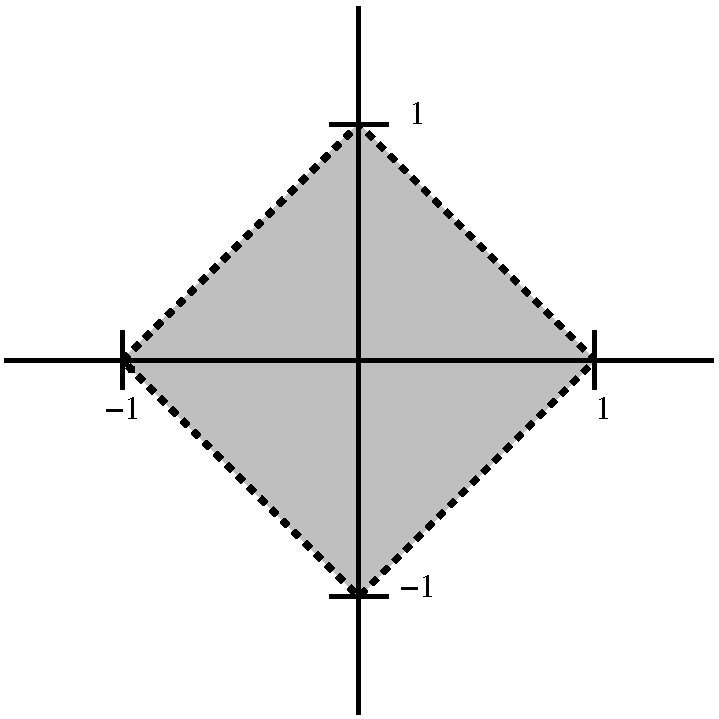
\includegraphics[height=6cm]{figs/ex_20_1_1}
  \end{center}
  Now we show that $d'$ is a metric and induces the usual topology of $\reals^n$.
  \qproof{
    It is easy to see that $d'$ meets the properties required of a metric.
    Clearly $d'(\vx, \vy) \geq 0$ since each $\abs{x_i - y_i} \geq 0$, and $d'(\vx, \vy) = 0$ if and only if each $x_i = y_i$ so that $\vx = \vy$.
    Also it is obvious that $d'(\vx, \vy) = d'(\vy, \vx)$ since each $\abs{x_i - y_i} = \abs{y_i - x_i}$.
    For the triangle inequality we simply have that
    \ali{
      d'(\vx, \vz) &= \sum_{i=1}^n \abs{x_i - z_i} \\
      &\leq \sum_{i=1}^n \parens{\abs{x_i - y_i} + \abs{y_i - z_i}} & \text{(since each $\abs{x_i-z_i} \leq \abs{x_i-y_i} + \abs{y_i-z_i}$)} \\
      &= \sum_{i=1}^n \abs{x_i - y_i} + \sum_{i=1}^n \abs{y_i - z_i} \\
      &= d'(\vx, \vy) + d'(\vy, \vz) \,.
    }

    We now show that the metric topology induced by $d'$ is the same as that induced by the square metric $\r$, which shows the desired result since the square metric induces the standard product topology on $\reals^n$ by Theorem~20.3.
    First consider any $\vx \in \reals^n$ and any $\e > 0$.
    Let $\d = \e$ and consider any $\vy \in B_{d'}(\vx, \d)$.
    Suppose also that $j$ is an index in $\intsfin{n}$ where
    \gath{
      \r(\vx, \vy) = \max\braces{\abs{x_1 - y_1}, \ldots, \abs{x_n - y_n}} = \abs{x_j - y_j} \,.
    }
    Since $\vy \in B_{d'}(\vx, \d)$, we have
    \gath{
      d'(\vx,\vy) = \sum_{i=1}^n \abs{x_i - y_i} < \d = \e \\
      \abs{x_j - y_j} + \sum_{i \neq j} \abs{x_i - y_i} < \e \\
      \abs{x_j - y_j} < \e - \sum_{i \neq j} \abs{x_i - y_i} \leq \e \\
      \r(\vx, \vy) < \e
    }
    since of course $\sum_{i \neq j} \abs{x_i - y_i} \geq 0$.
    Therefore $\vy \in B_\r(\vx,\e)$, which shows $B_{d'}(\vx, \d) \ss B_\r(\vx, \e)$ so that the metric topology of $d'$ is finer the the metric topology of $\r$ by Lemma~20.2.

    Now again consider and $\vx \in \reals^n$ and $\e > 0$, and this time let $\d = \e/n$.
    Consider any $\vy \in B_\r(\vx, \d)$ and again  suppose also that $j$ is an index in $\intsfin{n}$ where
    \gath{
      \r(\vx, \vy) = \max\braces{\abs{x_1 - y_1}, \ldots, \abs{x_n - y_n}} = \abs{x_j - y_j} \,.
    }
    We then have
    \gath{
      \abs{x_j - y_j} = \r(\vx, \vy) < \d = \e/n \\
      n \abs{x_j - y_j} < \e \,.
    }
    We also have
    \ali{
      d'(\vx, \vy) &= \sum_{i=1}^n \abs{x_i - y_i} \\
      &\leq \sum_{i=1}^n \abs{x_j - y_i} & \text{(since each $\abs{x_i - y_i} \leq \abs{x_j - y_j}$)} \\
      &= n \abs{x_j - y_j} \\
      &< \e
    }
    so that $\vy \in B_{d'}(\vx, \e)$.
    Hence $B_\r(\vx, \d) \ss B_{d'}(\vx, \e)$ so that the metric topology of $\r$ is also finer than that of $d'$ again by Lemma~20.2.
    Therefore it must be that the two topologies are equal since each is finer than the other.
  }

  (b) Let $d$ denote the metric defined in part (a), that is
  \gath{
    d(\vx, \vy) = \sum_{i=1}^n \abs{x_i - y_i} \,.
  }
  First we show that the metric topology induced by $d'$ is finer than that induced by $\rho$.
  So consider any $\vx \in \reals^n$ and $\e > 0$.
  Let $\d = \e$ and suppose that $\vy \in B_{d'}(\vx, \d)$ so that
  \gath{
    d'(\vx, \vy) = \parens{\sum_{i=1}^n \abs{x_i - y_i}^p}^{1/p} < \d = \e \,.
  }
  Suppose that $j$ is an index in $\intsfin{n}$ where
  \gath{
    \r(\vx, \vy) = \max\braces{\abs{x_1 - y_1}, \ldots, \abs{x_n - y_n}} = \abs{x_j - y_j} \,.
  }
  Then
  \gath{
    \abs{x_j - y_j}^p \leq \abs{x_j - y_j}^p + \sum_{i \neq j} \abs{x_i - y_i}^p = \sum_{i=1}^n \abs{x_i - y_i}^p
  }
  so that, by Corollary~\ref{cor:metric:opmon}, we have
  \gath{
    \parens{\abs{x_j - y_j}^p}^{1/p} \leq \parens{\sum_{i=1}^n \abs{x_i - y_i}^p}^{1/p} < \e \\
    \abs{x_j - y_j} < \e \\
    \r(\vx, \vy) < \e \,.
  }
  Therefore $\vy \in B_\r(\vx, \e)$ so that $B_{d'}(\vx, \d) \ss B_\r(\vx, \e)$.
  This suffices to show that the metric topology induced by $d'$ is finer than that induced by $\rho$ by Lemma~20.2.

  Now we show that the metric topology induced by $d$ is finer than that induced by $d'$.
  So again consider any $\vx \in \reals^n$ and $\e > 0$.
  Again let $\d = \e$ and suppose that $\vy \in B_d(\vx, \d)$ so that
  \gath{
    d(\vx, \vy) = \sum_{i=1}^n \abs{x_i - y_i} < \d = \e \,.
  }
  Then, since each $\abs{x_i - y_i} \geq 0$, we have by Lemma~\ref{lem:metric:polynom} that
  \ali{
    \sum_{i=1}^n \abs{x_i - y_i}^p &\leq \parens{\sum_{i=1}^n \abs{x_i - y_i}}^p \\
    \parens{\sum_{i=1}^n \abs{x_i - y_i}^p }^{1/p} &\leq \squares{\parens{\sum_{i=1}^n \abs{x_i - y_i}}^p}^{1/p} \\
    d'(\vx, \vy) &\leq \sum_{i=1}^n \abs{x_i - y_i} < \e \,,
  }
  where we have used Corollary~\ref{cor:metric:opmon} in the second step.
  Thus $\vy \in B_{d'}(\vx, \e)$ so that $B_d(\vx, \d) \ss B_{d'}(\vx, \e)$.
  This of course shows that the metric topology induced by $d$ is finer than that induced by $d'$ by Lemma~20.2 again.

  Thus we have shown that the metric topology induced by $d'$ is finer than that induced by $\r$, and also that that induced by $d$ is finer than that induced by $d'$.
  But it was shown in part (a) and Theorem~20.3 that those induced by $d$ and $\r$ are the same topology, which is is the usual product topology on $\reals^n$.
  Hence if $\cT_p$ denotes this usual product topology, we have
  \gath{
    \cT_p = \cT_\r \ss \cT_{d'} \ss \cT_d = \cT_\r = \cT_p \,.
  }
  So it must be that the metric topology induced by $d'$ is this topology as well as desired.
}


\exercise{2}{
  Show that $\reals \times \reals$ in the dictionary order topology is metrizable.
}
\sol{
    \qproof{
    In what follows let
    \gath{
      \bd(x,y) = \min\braces{\abs{x-y}, 1}
    }
    be the standard bounded metric on $\reals$, noting that this is a metric by Theorem~20.1.
    Now define the function $d : \reals^2 \times \reals^2 \to \reals$ by
    \gath{
      d(\vx, \vy) = \begin{cases}
        1 & x_1 \neq y_1 \\
        \bd(x_2, y_2) & x_1 = y_1 \,.
      \end{cases}
    }
    We claim that this is a metric on $\reals^2$ that induces the dictionary order topology.

    First we show that $d$ is a metric on $\reals^2$.
    Clearly $d(\vx, \vy) \geq 0$ since both $1 \geq 0$ and $\bd(x_2, y_2) \geq 0$ since $\bd$ is a metric.
    Moreover if $\vx = \vy$ then $x_1 = y_1$ and $x_2 = y_2$ so that $d(\vx, \vy) = \bd(x_2,y_2) = 0$.
    Conversely if $d(\vx, \vy) = 0$ then clearly $d(\vx, \vy) \neq 1$ so that it must be that $x_1 = y_1$ and $d(\vx, \vy) = \bd(x_2,y_2) = 0$ so that $x_2 = y_2$ since $\bd$ is a metric.
    From this it follows that $\vx = \vy$ since $x_1 = y_1$ and $x_2 = y_2$, which shows property (1) of a metric.

    It is also obvious that $d(\vx, \vy) = d(\vy, \vx)$ since if $x_1 \neq y_1$ then $d(\vx,\vy) = 1 = d(\vy, \vx)$.
    If $x_1 = x_2$ then $d(\vx, \vy) = \bd(x_2,y_2) = \bd(y_2,x_2) = d(\vy, \vx)$ since $\bd$ is a metric.
    This shows property (2) of a metric.
    Lastly, consider $\vx$, $\vy$, and $\vz$ in $\reals^2$.

    Case: $x_1 \neq z_1$.
    Then $d(\vx, \vz) = 1$ and it must be that either $y_1 \neq x_1$ or $y_1 \neq z_1$ since otherwise we would have that $x_1 = y_1 = z_1$.
    Thus either $d(\vx, \vy) = 1$ or $d(\vy, \vz) = 1$ and hence
    \gath{
      d(\vx, \vy) + d(\vy, \vz) \geq 1 = d(\vx, \vz)
    }
    since both $d(\vx, \vy) \geq 0$ and $d(\vy, \vz) \geq 0$.

    Case: $x_1 = z_1$.
    Then $d(\vx, \vz) = \bd(x_2,z_2)$.
    If $y_1 = x_1$ then $x_1 = y_1 = z_1$ so that
    \gath{
      d(\vx, \vz) = \bd(x_2,z_2) \leq \bd(x_2,y_2) + \bd(y_2,z_2) = d(\vx,\vy) + d(\vy,\vz)
    }
    since $\bd$ is a metric.
    If $y_1 \neq x_1$ then $y_1 \neq x_1 = z_1$, and hence $d(\vx, \vy) = d(\vy, \vz) = 1$ so that
    \gath{
      d(\vx, \vz) = \bd(x_2, z_2) \leq 1 \leq 2 = 1 + 1 = d(\vx, \vy) + d(\vy, \vz)
    }
    since $\bd$ is the bounded metric so that it is always at most 1.

    Thus in all cases we have shown property (3) of a metric.

    In what follows let $\prec$ denote the dictionary order on $\reals^2$.
    To show that $d$ induces the dictionary order topology, first consider any point $\vx \in \reals^2$ and any basis element $B$ of the dictionary order topology that contains $\vx$.
    Then of course $B = (\va, \vb)$, where $\va \prec \vx \prec \vb$ since the dictionary order has no largest or smallest elements in $\reals^2$.
    Now define
    \gath{
      \d_a = \begin{cases}
        1 & x_2 = a_2 \\
        \abs{x_2 - a_2} & x_2 \neq a_2
      \end{cases}
    }
    and
    \gath{
      \d_b = \begin{cases}
        1 & x_2 = b_2 \\
        \abs{x_2 - b_2} & x_2 \neq b_2 \,,
      \end{cases}
    }
    and let $\d = \min\braces{1, \d_a, \d_b}$.
    Clearly the set $B_d(\vx, \d)$ is a basis element of the topology induced by $d$, and we claim that $\vx \in B_d(\vx, \d) \ss B$.

    That $\vx \in B_d(\vx, \d)$ is obvious.
    So now consider any $\vy \in B_d(\vx, \d)$ so that $d(\vx, \vy) < \d \leq 1$.
    Hence it cannot be that $x_1 \neq y_1$ by definition, since $d(\vx, \vy) = 1$ in that case,  and so $x_1 = y_1$.
    If $x_2 = a_2$ then it has to be that $a_1 < x_1$ since otherwise it would not be the case that $\va \prec \vx$.
    Thus we have $a_1 < x_1 = y_1$ so that $\va \prec \vy$.

    On the other hand if $x_2 \neq a_2$ then it must be that $a_1 \leq y_1$ since otherwise we would have $x_1 = y_1 < a_1$ so that $\vx \prec \va$.
    If $a_1 < y_1 = x_1$ then of course $\va \prec \vy$ so assume that $a_1 = y_1 = x_1$.
    The it must be that $a_2 < x_2$ since $\va \prec \vx$, and so $\abs{x_2 - a_2} = x_2 - a_2$.
    Then, since $x_1 = y_1$, we have that $\bd(x_2, y_2) = d(\vx, \vy) < \d \leq 1$ so it must be that $d(\vx, \vy) = \bd(x_2, y_2) = \abs{x_2 - y_2}$.
    Also $\d_a = \abs{x_2 - a_2} = x_2 - a_2$ since $x_2 \neq a_2$.
    Hence we have $\abs{x_2 - y_2} = d(\vx, \vy) < \d \leq \d_a = x_2 - a_2$, from which it readily follows that $a_2 < y_2$ so that again $\va \prec \vy$.

    Therefore in all cases $\va \prec \vy$.
    Analogous arguments show that $\vy \prec \vb$ so that $\vy \in (\va, \vb) = B$, which shows that $B_d(\vx, \d) \ss B$ as desired since $\vy$ was arbitrary.
    This shows that the topology induced by $d$ is finer than the dictionary order topology by Lemma~13.3.

    Now again suppose that $\vx \in \reals^2$, and that $\e' > 0$ and $\vx' \in \reals^2$ such that $B_d(\vx', \e')$ is an arbitrary basis element of the metric topology induced by $d$ that contains $\vx$.
    It was shown after the definition of a metric topology in the text that there is another ball $B_d(\vx, \e)$ centered at $\vx$ such that $B_d(\vx, \e) \ss B_d(\vx', \e')$.
    Let $\d = \min\braces{1, \e}$ and define $\va = x_1 \times (x_2 - \d)$ and $\vb = x_1 \times (x_2 + \d)$.
    Set $B = (\va, \vb)$, which is clearly a basis element of the dictionary order topology.
    So consider any $\vy \in B$ so that $\va \prec \vy \prec \vb$.
    Clearly it must be that $a_1 = y_1 = b_1 = x_1$ since otherwise we would have that $\vy \prec \va$ or $\vb \prec \vy$.
    From this it follows that $a_2 = x_2 - \d < y_2 < x_2 + \d = b_2$ so that $-\d < y_2 - x_2 < \d$ and hence $\abs{x_2 - y_2} < \d$.
    Moreover, since $y_1 = x_1$ and $\d \leq 1$, it follows that $d(\vx, \vy) = \bd(x_2, y_2) = \abs{x_2 - y_2} < \d \leq \e$.
    This shows that $\vy \in B_d(\vx, \e)$, which shows that $B \ss B_d(\vx, \e) \ss B_d(\vx', \e')$ since $\vy$ was arbitrary.
    This proves that the dictionary order topology is finer than the topology induced by $d$ again by Lemma~13.3.

    Since each is finer than the other the topologies must be the same, which shows that the dictionary order topology is metrizable as desired.
  }
}

\exercise{3}{
  Let $X$ be metric space with metric $d$.
  \eparts{
  \item Show that $d : X \times X \to \reals$ is continuous.
  \item Let $X'$ denote a space having the same underlying set as $X$.
    Show that if $d : X' \times X' \to \reals$ is continuous, then the topology of $X'$ is finer than the topology of $X$.
  }
  One can summarize the result of this exercise as follows: If $X$ has a metric $d$, then the topology induced by $d$ is the coarsest topology relative to which the function $d$ is continuous.
}
\sol{
    (a) We use Theorem~18.1 part (4) to show that $d$ is continuous.
  So consider any $x_1 \times x_2 \in X \times X$ and any neighborhood $V$ of $z = d(x_1,x_2)$, noting that $V \ss \reals$ since $\reals$ is the range of $d$.
  Since $V$ is open in $\reals$, there is a basis element $B = (a,b)$ containing $z$ where $B \ss V$.
  Hence $a < z < b$.
  Now let $\e = \min\braces{(z-a)/2, (b-z)/2}$, noting that $\e > 0$ since $z > a$ and $b > z$.
  Next define $U_1 = B_d(x_1, \e)$ and $U_2 = B_d(x_2, \e)$ so that they are both basis elements and therefore open sets of the metric space $X$.
  It then follows that $U = U_1 \times U_2$ is a a basis element and therefore an  open set of the product space $X \times X$.
  Clearly we have that $x_1 \in B_d(x_1, \e) = U_1$ and $x_2 \in B_d(x_2, \e) = U_2$ so that $U$ contains $x_1 \times x_2$ and so is a neighborhood of $x_1 \times x_2$.

  We claim that $d(U) \ss B$.
  To see this, consider any $w \in d(U)$ so that there is a $y_1 \times y_2 \in U = U_1 \times U_2$ such that $w = d(y_1, y_2)$.
  Therefore $y_1 \in U_1 = B_d(x_1, \e)$ so that $d(y_1, x_1) < \e$, and similarly $d(y_2, x_2) < \e$ since $y_2 \in U_2 = B_d(x_2, \e)$.
  Then, since $d$ is a metric, we have
  \ali{
    z = d(x_1, x_2) &\leq d(x_1, y_1) + d(y_1, x_2) \\
    &\leq d(x_1, y_1) + d(y_1, y_2) + d(y_2, x_2) \\
    &= d(y_1, x_1) + d(y_1, y_2) + d(y_2, x_2) \\
    &< \e + w + \e \\
    z &< w + 2\e \leq w + 2(z-a)/2 = w + z - a \\
    a &< w \,.
  }
  Similarly, we have
  \ali{
    w = d(y_1, y_2) &\leq d(y_1, x_1) + d(x_1, y_2) \\
    &\leq d(y_1, x_1) + d(x_1, x_2) + d(x_2, y_2) \\
    &= d(y_1, x_1) + d(x_1, x_2) + d(y_2, x_2) \\
    &< \e + z + \e \\
    w &< z + 2\e \leq z + 2(b-z)/2 = z + b - z \\
    w &< b \,.
  }
  We therefore have that $a < w < b$ so that $w \in (a,b) = B$.
  This of course shows that $d(U) \ss B$ since $w$ was arbitrary.
  Moreover, we have that $B \ss V$ so that clearly $d(U) \ss V$, which completes the proof of Theorem~18.1 part (4) so that $d$ is continuous.

  (b) Let $U$ be any open set of $X$ and consider any $x \in U$.
  Then clearly there is a basis element $B_d(y, \e)$, for some $\e > 0$ and $y \in U$, of the metric topology $X$ that contains $x$ and where $B_d(y, \e) \ss U$.
  Now, since $d$ is continuous with respect to $X' \times X'$, it follows from Exercise~18.11 that the function $d_y(z) = d(y,z)$ is a continuous function from $X'$ to $\reals$.
  Since clearly the interval $(-\infty, \e)$ is open in $\reals$, it then follows that the set
  \gath{
    \inv{d_y}((-\infty, \e)) = \braces{z \in X' \where d_y(z) < \e} = \braces{z \in X \where d(y, z) < \e} = B_d(y, \e)
  }
  is also open in $X'$.
  Thus $B_d(y,\e)$ is an open set in $X'$ containing $x$ such that $B_d(y, \e) \ss U$.
  This shows that $U$ is also open in $X'$ by Exercise~13.1 since the point $x \in U$ was arbitrary.
  This suffices to show the desired result.
}

\exercise{4}{
  Consider the product, uniform, and box topologies on $\reals^\w$,
  \eparts{
  \item In which topologies are the following functions from $\reals$ to $\reals^\w$ continuous?
    \ali{
      f(t) &= (t, 2t, 3t, \ldots), \\
      g(t) &= (t, t, t, \ldots), \\
      h(t) &= (t, \tfrac{1}{2}t, \tfrac{1}{3}t, \ldots).
    }
  \item In which topologies do the following sequences converge?
    \ali{
      \vw_1 &= (1,1,1,1,\ldots), & \vx_1 &= (1,1,1,1, \ldots), \\
      \vw_2 &= (0,2,2,2,\ldots), & \vx_2 &= (0,\tfrac{1}{2},\tfrac{1}{2},\tfrac{1}{2}, \ldots), \\
      \vw_3 &= (0,0,3,3,\ldots), & \vx_3 &= (0,0,\tfrac{1}{3},\tfrac{1}{3}, \ldots), \\
      &\ldots & &\ldots \\
      \vy_1 &= (1,0,0,0,\ldots), & \vz_1 &= (1,1,0,0, \ldots), \\
      \vy_2 &= (\tfrac{1}{2},\tfrac{1}{2},0,0,\ldots), & \vz_2 &= (\tfrac{1}{2},\tfrac{1}{2},0,0, \ldots), \\
      \vy_3 &= (\tfrac{1}{3},\tfrac{1}{3},\tfrac{1}{3},0,\ldots), & \vz_3 &= (\tfrac{1}{3},\tfrac{1}{3},0,0, \ldots), \\
      &\ldots & &\ldots
    }
  }
}
\sol{
    \begin{lem}\label{lem:metric:ball}
    Suppose that $X$ is a metric space with metric $d$.
    If $U$ is an open set of $X$ containing a point $x$ then there is a ball $B_d(x, \e)$ centered at $x$ that is contained in $U$.
  \end{lem}
  \qproof{
    The main part of this proof was given after the definition of a metric topology in the text, but we repeat it here for completeness.

    By the definition of the metric topology, there is a $\d > 0$ and $y \in X$ such that the basis element $B_d(y,\d)$ contains $x$ and is contained in $U$.
    Let $\e = \d - d(x,y)$ so that $d(x,y) = \d - \e$, noting that $\e > 0$ since $x \in B_d(y, \d)$ so that $d(x,y) < \d$.
    Then, for any $z \in B_d(x, \e)$, we have that $d(z,x) < \e$ and so
    \gath{
      d(z,y) \leq d(z,x) + d(x,y) = d(z,x) + \d - \e < \e + \d - \e = \d
    }
    since $d$ is a metric.
    Hence $z \in B_d(y, \d)$ so that $B_d(x,\e) \ss B_d(y, \d) \ss U$ as desired since $z$ was arbitrary.
  }

  \begin{lem}\label{lem:metric:finer}
    Suppose that $X$ is a topological space and $Y$ and $Y'$ are topological spaces on the same set, and that $Y'$ is finer than $Y$.
    Suppose also that $f: X \to Y$ so that of course it is also a function from $X$ to $Y'$.
    We assert the following:
    \lparts{
    \item If $f$ is continuous with respect to $Y'$ then it is also continuous with respect to $Y$.
    \item If $f$ is \emph{not} continuous with respect to $Y$ then it is also not continuous with respect to $Y'$.
    \item If a sequence in $Y'$ converges to a point $y_0$, then it also converges to $y_0$ in $Y$.
    \item If a sequence in $Y$ does not converge to a point $y_0$, then it also does not converge to $y_0$ in $Y'$.
    \item If a sequence in $Y$ does not converge at all, then it also does not converge at all in $Y'$.
    \item If $Y$ is a Hausdorff space, then so is $Y'$.
    }
  \end{lem}
  \qproof{
    For assertion (1) suppose that $f$ is continuous with respect to $Y'$ and let $U$ be any open set of $Y$.
    Since $Y'$ is finer than $Y$, it follows that $U$ is also open in $Y'$.
    Then, since $f$ is continuous with respect to $Y'$ we have that $\inv{f}(U)$ is open in $X$, which suffices to show that $f$ is continuous with respect to $Y$ since $U$ was an arbitrary open set. Assertion (2) follows immediately from the contrapositive of (1).

    Regarding (3), suppose that a sequence $\seqinf{y}$ converges to $y_0$ in $Y'$ and let $U$ be any neighborhood of $y_0$ in $Y$.
    Then $U$ is also open in $Y'$ since it is finer than $Y$, hence $U$ is a neighborhood of $y_0$ in $Y'$.
    Thus there is an $N \in \pints$ such that $x_n \in U$ for all $n \geq N$, since the sequence converges to $y_0$ in $Y'$.
    Since $U$ was an arbitrary neighborhood of $Y$, this shows that the sequence converges to $y_0$ in $Y$.
    Assertion (4) follows immediately from the contrapositive of (3).
    Assertion (5) then immediately follows from (4) since, if a sequence does not converge at all in $Y$ then for any point $y_0 \in Y$, it does not converge to $y_0$.
    Then it also does not converge to $y_0$ in $Y'$ by (4).
    Since $y_0$ was arbitrary, this shows that it does not converge at all in $Y'$.

    For (6), suppose that $Y$ is a Hausdorff space and let $x$ and $y$ be distinct points of $Y'$ so that they are of course also points of $Y$.
    Hence there are neighborhoods $U$ and $V$ of $x$ and $y$, respectively, in $Y$ that are disjoint.
    Since $Y'$ is finer than $Y$, we have that $U$ and $V$ are also open sets of $Y'$ and thus are disjoint neighborhoods of $x$ and $y$ in $Y'$ as well.
    This suffices to show that $Y'$ is Hausdorff as desired.
  }

  \mainprob
  
  (a) Regarding whether or not the functions are continuous in the various topologies, we claim the following:
  \begin{center}
    \begin{tabular}{c|ccc}
      & Product & Uniform & Box \\
      \hline
      $f$ & Yes & No & No \\
      $g$ & Yes & Yes & No \\
      $h$ & Yes & Yes & No
    \end{tabular}
  \end{center}

  \qproof{
    First, the functions $f$, $g$, and $h$ can all be considered as special cases of the more general function
    \gath{
      s(t) = (s_n(t))_{n \in \pints} \,,
    }
    where each $s_n(t) = \a_n t$, and $\a_n = n$ for $f$, $\a_n = 1$ for $g$, and $\a_n = 1/n$ for $h$.

    Clearly each $s_n$ is continuous for the three $\a_n$ by elementary calculus so that $s$ is continuous in the product topology by Theorem~19.6 for all three $\a_n$.
    We can show that $s$ is \emph{not} continuous in the box topology for all three $\a_n$ with a single example.
    Consider the set $B = \prod_{n \in \pints} (-1/n^2, 1/n^2)$, which is clearly a basis element of the box topology and so is open.
    Similar to Example~19.2, if $s$ were continuous then there would be an interval $(-\d, \d)$ about the point $0$ such that $s((-\d, \d)) \ss B$, where of course $\d > 0$.
    This would of course mean that
    \gath{
      s_n((-\d, \d)) = (-\a_n \d, \a_n \d) \ss (-1/n^2, 1/n^2)
    }
    for all $n \in \pints$.
    However, since clearly there is an $n \in \pints$ large enough that
    \gath{
      n^3 \d \geq n^2 \d \geq n \d > 1 \,,
    }
    we have that
    \gath{
      n\d \geq \d \geq \d/n > 1/n^2 \,,
    }
    and hence for all three functions we have that $\a_n \d > 1/n^2$ so that
    \gath{
      s_n((-\d,\d)) = (-\a_n\d, \a_n \d) \nss (-1/n^2, 1/n^2) \,.
    }
    This shows that $s$ cannot be continuous with respect to the box topology for all three $\a_n$.

    Next we show that $f$ is \emph{not} continuous in the uniform topology.
    First, suppose that $\br$ is the metric that induces the uniform topology, i.e.
    \gath{
      \br(\vx, \vy) = \sup\braces{\bd(x_n, y_n) \where n \in \pints} \,.
    }
    Now consider the basis element and open set $B_{\br}(\vze, 1)$ in the uniform topology.
    If $f$ were continuous then there would be a $\d > 0$ such that
    \gath{
      f((-\d, \d)) = \prod_{n \in \pints} (-\d n, \d n) \ss B_{\br}(\vze, 1) \,.
    }
    Clearly there is an $n \in \pints$ large enough such that $n > 1/\d$ so that $\d n > 1$.
    Then consider the point $\vx \in \reals^\w$ defined by
    \gath{
      x_m = \begin{cases}
        0 & m \neq n+1 \\
        \d n & m = n+1 \,.
      \end{cases}
    }
    We then have of course that $-(n+1)\d < 0 < n\d = x_{n+1} < (n+1)\d$ so that $x_{n+1} \in (-(n+1)\d, (n+1)\d)$.
    It then follows that $\vx \in f((-\d, \d)$.
    However, we also have that $\bd(\d n, 0) = \max\braces{\abs{\d n - 0}, 1} = \max\braces{\d n, 1} = 1$ since $\d n > 1$.
    Hence it is not true that $\br(\vx, \vze) < 1$ so that $\vx \notin B_{\br}(\vze, 1)$.
    Thus $f((-\d, \d)) \nss B_{\br}(\vze, 1)$ so that $f$ is not continuous in the uniform topology.

    Next we show that $g$ and $h$ \emph{are} continuous in the uniform topology at the same time, which we show using Theorem~18.1 part (4).
    Consider any real $u$ and any neighborhood $V$ of $\vx = g(u)$ (or $\vx = h(u)$) in the uniform topology.
    Then by Lemma~\ref{lem:metric:ball} there is an $\e > 0$ such that the basis element $B_{\br}(\vx, \e)$ is a subset of $V$.
    Now consider the basis element and open set $U = B_d(u, \e/2)$, where $d$ denotes the usual metric on $\reals$.
    Obviously $U$ contains $u$ but we also claim that $g(U) \ss V$ (or $h(U) \ss V$), thereby completing the proof.

    So consider any $\vy \in g(U)$ (or $\vy \in h(U)$) so that there is some $v \in U$ such that $\vy = g(v)$ (or $\vy = h(v)$)
    In the case of $g$ we have that $\vx = g(u) = (u,u,u,\ldots)$, which is to say that $x_n = u$ for all $n \in \pints$.
    Similarly $y_n = v$ for all $n \in \pints$ since $\vy = g(v)$.
    Now, since $v \in U = B_d(u,\e/2)$, we have that
    \gath{
      \bd(y_n, x_n) \leq d(y_n, x_n) = d(v, u) < \e/2
    }
    for all $n \in \pints$.
    From this it follows that
    \gath{
      \br(\vy, \vx) = \sup\braces{\bd(y_n, x_n) \where n \in \pints} \leq \e/2 < \e \,.
    }
    Likewise in the case of $h$ we have that $x_n = u/n$ and $y_n = v/n$ for all $n \in \pints$ since $\vx = h(u)$ and $\vy = h(v)$.
    We therefore have that
    \gath{
      \bd(y_n, x_n) \leq d(y_n, x_n) = \abs{y_n - x_n} = \abs{v/n - u/n} = \abs{\frac{v-u}{n}} = \frac{1}{n}\abs{v-u} = \frac{1}{n}d(v,u) < \frac{\e/2}{n} \leq \e/2
    }
    for all $n \in \pints$ since every $n \geq 1$.
    Hence again
    \gath{
      \br(\vy, \vx) = \sup\braces{\bd(y_n, x_n) \where n \in \pints} \leq \e/2 < \e \,.
    }
    Therefore for both functions we have $\br(\vy, \vx) < \e$ so that $\vy \in B_{\br}(\vx, \e)$.
    This shows that $g(U) \ss B_{\br}(\vx, \e) \ss V$ (or $h(U) \ss B_{\br}(\vx, \e) \ss V$) as desired since $\vy$ was arbitrary.
  }

  (b) First we note that, since $\reals$ is a Hausdorff space, $\reals^\w$ is as well in both the box and product topologies by Theorem~19.4.
  Therefore the uniform topology on $\reals^\w$ is also Hausdorff by Lemma~\ref{lem:metric:finer} part (6) since it is finer than the product topology.
  It then follows from Theorem~17.10 that if any of the sequences converge in any of the three topologies, then they converge to a unique point.

  Regarding whether the sequences converge in the various topologies then, we claim
    \begin{center}
    \begin{tabular}{c|ccc}
      & Product & Uniform & Box \\
      \hline
      $\vw$ & Yes & No & No \\
      $\vx$ & Yes & Yes & No \\
      $\vy$ & Yes & Yes & No \\
      $\vz$ & Yes & Yes & Yes
    \end{tabular}
  \end{center}
  \qproof{
    Now, regarding the $\vw$ sequence, each element in the sequence is defined as
    \gath{
      \vw_n = (w_{n,1}, w_{n,2}, w_{n,3}, \ldots) \,,
    }
    where
    \gath{
      w_{n,m} = \begin{cases}
        0 & m < n \\
        n & m \geq n
      \end{cases}
    }
    for $n,m \in \pints$.

    First we show that the $\vw$ sequence converges to the point $\vze$ in the product topology.
    So consider any neighborhood $U$ of $\vze$ in the product topology so that there is a basis element $B$ containing $\vze$ where $B \ss U$.
    Then $B = \prod_{m=1}^\infty B_m$ where each $B_m$ is open and $B_m$ is all of $\reals$ for all but finitely many values of $m$.
    Let $J$ then be a finite subset of $\pints$ where each $B_m = \reals$ for $m \notin J$.
    Of course we also have that $0 \in B_m$ for all $m \in \pints$ since $B$ contains $\vze$.

    Then $J$ has a largest element $N$ since it is a finite set of positive integers.
    Now consider any $n \geq N+1$ and any $m \in \pints$.
    If $m \in J$ then we have that $m \leq N < N+1 \leq n$ since $N$ is the largest element of $J$, and hence $w_{n,m} = 0 \in B_m$.
    If $m \notin J$ then of course $B_m = \reals$ so that of course $w_{n,m} \in \reals = B_m$ regardless of whether $w_{n,m} = 0$ or $w_{n,m} = n$.
    Hence either way we have $w_{n,m} \in B_m$, which shows that $\vw_n \in \prod_{m=1}^\infty B_m = B$ since $m$ was arbitrary.
    Thus also $\vw_n \in U$ since $B \ss U$.
    Since $n \geq N+1$ was arbitrary and $U$ was an arbitrary neighborhood of $\vze$, this shows that the sequence converges to $\vze$ as desired.
    
    Next we show that the $\vw$ sequence does not converge in the uniform topology.
    It suffices to show that the sequence does not converge to $\vze$, since if it converged to any other point $\vx$, then by Lemma~\ref{lem:metric:finer} part (3) it would also converge to $\vx$ in the product topology since it is coarser than the uniform topology.
    However, this would violate the fact that the sequence converges to $\vze$ in the product topology (just shown above), and so cannot also converge to $\vx \neq \vze$ since the convergence point is unique as noted above.

    So consider the neighborhood $B_{\br}(\vze, 1)$ of $\vze$ in the uniform topology.
    We claim that no elements of the sequence are in this neighborhood so that it clearly cannot converge to $\vze$.
    So consider any $n \in \pints$ so that we clearly have $w_{n,n} = n \geq 1 > 0$.
    Therefore $d(w_{n,n}, 0) = \abs{w_{n,n} - 0} = \abs{w_{n,n}} = w_{n,n} \geq 1$, from which it follows that it has to be that $\bd(w_{n,n}, 0) = 1$.
    This of course implies that
    \gath{
      \br(\vw_n, \vze) = \sup\braces{\bd(w_{n,m}, 0) \where m \in \pints} \geq 1 \,.
    }
    Hence it is not true that $\br(\vw_n, \vze) < 1$ so that $\vw_n \notin B_{\br}(\vze, 1)$.
    This shows the desired result since $n$ was arbitrary.

    It then follows that the $\vw$ sequence also does not converge at all in the box topology by Lemma~\ref{lem:metric:finer} part (5) since it is finer than the uniform topology.

    Regarding the $\vx$ sequence, the definition is that each
    \gath{
      \vx_n = (x_{n,1}, x_{n,2}, x_{n,3}, \ldots) \,,
    }
    where
    \gath{
      x_{n,m} = \begin{cases}
        0 & m < n \\
        1/n & m \geq n
      \end{cases}
    }
    for $n,m \in \pints$.

    First we show that this sequence converges to $\vze$ in the uniform topology, which is of course is the unique convergence point.
    So consider any neighborhood $U$ of $\vze$ in the uniform topology so that by Lemma~\ref{lem:metric:ball} there is an $\e > 0$ where $B_{\br}(\vze, \e) \ss U$.
    Then there is a positive integer $N$ large enough so that $N > 2/\e$ so that, for any $n \geq N$ we have $1/n \leq 1/N < \e/2$.
    Next consider any such $n \geq N$ and any $m \in \pints$.
    Since $x_{n,m}$ is either $0$ or $1/n$ we have that $\abs{x_{n,m}} = x_{n,m} \leq 1/n$ so that
    \gath{
      \bd(x_{n,m}, 0) \leq d(x_{n,m}, 0) = \abs{x_{n,m} - 0} = \abs{x_{n,m}} = x_{n,m} \leq 1/n < \e/2 \,.
    }
    Thus, since $m$ was arbitrary, it follows that
    \gath{
      \br(\vx_n, \vze) = \sup\braces{\bd(x_{n,m}, 0) \where m \in \pints} \leq \e/2 < \e \,,
    }
    and hence $\vx_n \in B_{\br}(\vze, \e)$.
    Thus also $\vx_n \in U$ since $B_{\br}(\vze, \e) \ss U$.
    Since $n \geq N$ was arbitrary as was the neighborhood $U$, this shows that the sequence converges to $\vze$ as desired.

    Since it is coarser than the uniform topology, it follows that the $\vx$ sequence also converges to $\vze$ in the product topology as well by Lemma~\ref{lem:metric:finer} part (3).

    Next we show that the $\vx$ sequence does not converge in the box topology, for which it suffices to show that it does not converge to $\vze$.
    Again, this is because, if it were to converge to some other point $\vy \neq 0$ in the box topology, then it would also converge to $\vy$ in the uniform topology since it is coarser (Lemma~\ref{lem:metric:finer} part (3)), but this would violate the fact that it converges to the unique point $\vze$ by what was just shown.
    So consider the basis element and open set of the box topology $U = \prod_{n=1}^\infty U_n$ where each $U_n = (-1/n, 1/n)$.
    Clearly $U$ contains $\vze$ so that it is a neighborhood of $\vze$.
    We claim that no element of the sequence is in $U$, which of course suffices to show that it cannot converge to $\vze$.
    So consider any $n \in \pints$ and so that $x_{n,n} = 1/n \geq 1/n$ so that $x_{n,n} \notin (-1/n, 1/n) = U_n$.
    From this it follows that $\vx_n \notin \prod_{n=1}^\infty U_n = U$.
    Since $n$ was arbitrary this shows no element of the sequence is in $U$ so that the sequence cannot converge to $\vze$.

    Regarding the $\vy$ sequence, it is defined as
    \gath{
      \vy_n = (y_{n,1}, y_{n,2}, y_{n,3}, \ldots) \,,
    }
    where
    \gath{
      y_{n,m} = \begin{cases}
        1/n & m \leq n \\
        0 & m > n
      \end{cases}
    }
    for $n,m \in \pints$.
    Since $y_{n,m}$ is always either $0$ or $1/n$, the same argument that shows that the $\vx$ sequence converges to $\vze$ in the uniform topology shows that the $\vy$ sequence does as well.
    Of course this also mean that it converges to $\vze$ in the product topology as well since it is coarser.
    Similarly, the same argument that shows that the $\vx$ sequence does not converge in the box topology applies to $\vy$ as well since we have that $y_{n,n} = x_{n,n} = 1/n$ for all $n \in \pints$.

    Now, the $\vz$ sequence is defined by
    \gath{
      \vz_n = (z_{n,1}, z_{n,2}, z_{n,3}, \ldots) \,,
    }
    where
    \gath{
      z_{n,m} = \begin{cases}
        1/n & m \leq 2 \\
        0 & m > 2
      \end{cases}
    }
    for $n,m \in \pints$.

    We show that this sequence converges to $\vze$ in the box topology.
    So consider any neighborhood $U$ of $\vze$ in the box topology so that there is a basis element $B = \prod_{m=1}^\infty B_m$ containing $\vze$ where $B \ss U$.
    Of course then each $B_m$ is open in $\reals$ and $0 \in B_m$.
    Considering the standard topology of $\reals$ using the metric topology basis, there is then an $\e_1 > 0$ such that $B_d(0, \e_1) \ss B_1$ by Lemma~\ref{lem:metric:ball} since $B_1$ is open and contains $0$.
    Likewise there is an $\e_2 > 0$ where $B_d(0, \e_2) \ss B_2$.
    So set $\e = \min\braces{\e_1, \e_2}$ so that of course there is a positive integer $N$ large enough that $N > 1/\e$.
    Then, for any $n \geq N$ we have that $n \geq N > 1/\e$ so that $1/n < \e \leq \e_1$, and similarly $1/n < \e \leq \e_2$.
    Now consider any $m \in \pints$.
    If $m \leq 2$ then of course either $m = 1$ or $m = 2$ so that, either way, we have
    \gath{
      d(z_{n,m}, 0) = \abs{z_{n,m} - 0} = \abs{z_{n,m}} = \abs{1/n} = 1/n < \e \leq \e_m
    }
    so that $z_{n,m} \in B_d(0, \e_m) \ss B_m$.
    If $m > 2$ then we clear have $z_{n,m} = 0 \in B_m$ as well.
    Since $m$ was arbitrary, this shows that $\vz_n \in \prod_{m=1}^\infty B_m = B \ss U$.
    This shows that the sequence converges to $\vze$ since $n \geq N$ was arbitrary and $U$ was any neighborhood of $\vze$.

    Of course this also shows that the $\vz$ sequence converges to $\vze$ in the uniform and product topologies as well by Lemma~\ref{lem:metric:finer} part (3) since they are both coarser than the box topology.
  }
}

\exercise{5}{
  Let $\rinf$ be the subset of $\reals^\w$ consisting of all sequences that are eventually zero.
  What is the closure of $\rinf$ in $\reals^\w$ in the uniform topology?
  Justify your answer. 
}
\sol{
    Let $\reals^0$ denote the subset of $\reals^\w$ consisting of all sequences that converge to zero.
  We then claim that $\closure{\rinf} = \reals^0$, i.e. the closure of $\rinf$ is $\reals^0$.
  \qproof{
    $(\ss)$ We show this by contrapositive.
    So suppose that $\vx \notin \reals^0$ so that the sequence $\vx$ does \emph{not} converge to zero.
    Then there is a neighborhood $V$ of $0$ in the standard topology on $\reals$ such that, for any $N \in \pints$, there is an $n \geq N$ where $x_n \notin V$.
    It also follows from Lemma~\ref{lem:metric:ball} that there is an $\e > 0$ such that $B_d(0, \e) \ss V$.
    So let $\d = \min\braces{\e, 1}$ and consider the set $B_{\br}(\vx, \d)$, which is clearly a neighborhood of $\vx$ in the uniform topology.
    Also suppose that $\vy$ is any element of $\rinf$ so that $\vy$ is eventually zero.
    Then there must be an $N$ where $y_n = 0$ for all $n \geq N$.
    From before we have that there is a specific $n \geq N$ where $x_n \notin V$ so that also $x_n \notin B_d(0, \e)$, and thus
    \gath{
      d(y_n, x_n) = d(0, x_n) = d(x_n, 0) \geq \e \geq \d \,.
    }
    Then we have that both $d(y_n, x_n) \geq \d$ and $1 \geq \d$ so that
    \gath{
      \bd(y_n, x_n) = \min\braces{d(y_n, x_n), 1} \geq \d \,.
    }
    From this it clearly follows that
    \gath{
      \br(\vy, \vx) = \sup\braces{\bd(y_n, x_n) \where n \in \pints} \geq \d
    }
    so that $\vy \notin B_{\br}(\vx, \d)$.
    Since $\vy$ was arbitrary, this shows that $B_{\br}(\vx, \d)$ does not intersect $\rinf$.
    This in turn shows that $\vx$ is not a limit point of $\rinf$.
    Now, clearly also $\vx$ cannot be eventually zero since then it would converge to zero, hence $\vx \notin \rinf$ either.
    Therefore $\vx$ cannot be in the closure of $\rinf$.
    Hence by the contrapositive we have that $\closure{\rinf} \ss \reals^0$.

    $(\sps)$ Now consider any $\vx \in \reals^0$ so that the sequence $\vx$ converges to zero.
    Consider any neighborhood $U$ of $\vx$ in the uniform topology so that, by Lemma~\ref{lem:metric:ball}, there is an $\e > 0$ such that $B_{\br}(\vx, \e) \ss U$.
    Now, since $B_d(0, \e/2)$ is a neighborhood of $0$, it follows that there is an $N \in \pints$ where $x_n \in B_d(0, \e/2)$ for all $n \geq N$ since $\vx$ converges to $0$.
    Now define the sequence $\vy$ where
    \gath{
      y_n = \begin{cases}
        x_n & n < N \\
        0 & n \geq N
      \end{cases}
    }
    for $n \in \pints$.
    Clearly $\vy$ is eventually zero so that $\vy \in \rinf$.

    We also claim that $\vy \in U$.
    To see this consider any $n \in \pints$.
    If $n < N$ then clearly $y_n = x_n$ so that
    \gath{
      \bd(y_n, x_n) \leq d(y_n, x_n) = d(x_n, x_n) = 0 < \e/2 \,.
    }
    If $n \geq N$ then $y_n = 0$ and we have from before that $x_n \in B_d(0, \e/2)$ and hence
    \gath{
      \bd(y_n, x_n) \leq d(y_n, x_n) = d(0, x_n) = d(x_n, 0) < \e/2 \,.
    }
    Hence it follows that
    \gath{
      \br(\vy, \vx) = \sup\braces{\bd(y_n, x_n) \where n \in \pints} \leq \e/2 < \e
    }
    so that $\vy \in B_{\br}(\vx, \e) \ss U$.
    This shows that $\vy \in \rinf \cap U$.
    If $\vy = \vx$ then of course $\vx = \vy \in \rinf$ itself.
    If $\vy \neq \vx$ then we have shown that $\vx$ is a limit point of $\rinf$ since $U$ was an arbitrary neighborhood.
    Thus either way $\vy \in \closure{\rinf}$ so that $\closure{\rinf} \sps \reals^0$ since $\vx$ was arbitrary.
  }
  Lastly, we note that $\rinf$ is a proper subset of its closure $\closure{\rinf} = \reals^0$ since, for example, the sequence $\vx$ defined by $x_n = 1/n$ for all $n \in \pints$ clearly converges to zero so is in $\reals^0$ but is not eventually zero so is not in $\rinf$.
}

\exercise{6}{
  Let $\br$ be the uniform metric on $\reals^\w$.
  Given $\vx = \seqinf{x} \in \reals^\w$ and given $0 < \e < 1$, let
  \gath{
    U(\vx, \e) = (x_1-\e, x_1+\e) \times \cdots \times (x_n - \e, x_n + \e) \times \cdots \,.
  }
  \eparts{
  \item Show that $U(\vx, \e)$ is not equal to the $\e$-ball $B_{\br}(\vx, \e)$.
  \item Show that $U(\vx, \e)$ is not even open in the uniform topology.
  \item Show that
    \gath{
      B_{\br}(\vx, \e) = \bigcup_{\d < \e} U(\vx, \d) \,.
    }
  }
}
\sol{
    (a)
  \qproof{
    We show that $B_{\br}(\vx, \e)$ is not a subset of $U(\vx, \e)$, which of course suffices to show that they cannot be equal.
    To this end we define the point $\vy$ in $\reals^\w$ by
    \gath{
      y_n = x_n + \e\parens{1 - \frac{1}{n}}
    }
    for any $n \in \pints$.
    Then, for any such $n$, we clearly have that
    \ali{
      n &\geq 1 \\
      -n &\leq -1 < 0 \\
      -1 &\leq -\frac{1}{n} < 0 & \text{(since $n > 0$)} \\
      0 &\leq 1 - \frac{1}{n} < 1 \\
      0 &\leq \e\parens{1 - \frac{1}{n}} < \e & \text{(since $\e > 0$)} \\
      x_n &\leq x_n + \e\parens{1 - \frac{1}{n}} < x_n + \e \\
      x_n - \e < x_n &\leq y_n < x_n + \e
    }
    so that $y_n \in (x_n - \e, x_n + \e)$.
    Since $n$ was arbitrary, this shows that $\vy \in \prod_{n=1}^\infty (x_n - \e, x_n + \e) = U(\vx, \e)$.
    However, again for any $n \in \pints$, it was shown that $x_n \leq y_n$  so that
    \gath{
      d(y_n, x_n) = \abs{y_n - x_n} = y_n - x_n = x_n + \e\parens{1 - \frac{1}{n}} - x_n = \e\parens{1 - \frac{1}{n}} \,.
    }
    It was shown above that
    \ali{
      0 \leq \e\parens{1 - \frac{1}{n}} < \e &< 1 \\
      0 \leq d(y_n, x_n) < \e &< 1
    }
    so that
    \gath{
      \bd(y_n, x_n) = \min\braces{d(y_n, x_n), 1} = d(y_n, x_n) \,.
    }
    We then clearly have
    \gath{
      \lim_{n \to \infty} \bd(y_n, x_n) = \lim_{n \to \infty} d(y_n, x_n) = \lim_{n \to \infty} \e \parens{1 - \frac{1}{n}} = \e
    }
    so that
    \gath{
      \br(\vy, \vx) = \sup_{n \in \pints} \bd(y_n, x_n) = \e \geq \e
    }
    since the sequence $\vy$ is clearly monotonically increasing.
    This shows that $\vy \notin B_{\br}(\vx, \e)$ so that $B_{\br}(\vx, \e)$ cannot be a subset of $U(\vx, \e)$.
  }

  (b)
  \qproof{
    Let $\vy$ be the point in $\reals^\w$ defined in part (a) so that we know that $\vy \in U(\vx, \e)$.
    Now if $U(\vx, \e)$ were open in the uniform topology then there would be a basis element $B_{\br}(\vy, \d)$ that is contained in $U(\vx, \e)$.
    We shall show that any such basis element cannot be contained within $U(\vx, \e)$, from which the desired result follows.

    So consider any $\d > 0$ so that there is an $n \in \pints$ large enough that $n > \e/\d$.
    Then we have
    \ali{
      n &> \frac{\e}{\d} \\
      \d &> \e \frac{1}{n} & \text{(since both $\d > 0$ and $n > 0$)} \\
      -\e\frac{1}{n} + \d &> 0 \\
      \e - \e\frac{1}{n} + \d &> \e \\
      x_n + \e\parens{1 - \frac{1}{n}} + \d &> x_n + \e \\
      y_n + \d &> x_n + \e \,.
    }
    Now define the point $\vz$ by
    \gath{
      z_m = \begin{cases}
        y_m & m \neq n \\
        \frac{(x_n + \e) + (y_n + \d)}{2} & m = n \,.
      \end{cases}
    }
    It then follows that $x_n + \e < z_n < y_n + \d$.
    The fact that $x_n + \e < z_n$ means that of course $z_n \notin (x_n - \e, x_n + \e)$ so that $\vz \notin \prod_{m=1}^\infty (x_m - \e, x_m + \e) = U(\vx, \e)$.
    However, for $m \neq n$ we have that
    \gath{
      d(z_m, y_m) = d(y_m, y_m) = 0
    }
    and so $\bd(z_m, y_m) = 0$ as well.
    For $m = n$ we have
    \gath{
      x_m + \e = x_n + \e < z_m = z_n < y_n + \d = y_m + \d \\
      x_m + \e - y_m < z_m - y_m < \d \\
      x_m + \e - x_m - \e\parens{1 - \frac{1}{n}} < z_m - y_m < \d \\
      0 < \e\frac{1}{n} < z_m - y_m < \d \\
      \abs{z_m - y_m} < \d \\
      \bd(z_m, y_m) \leq d(z_m, y_m) < \d \,.
    }
    From these facts it follows that
    \gath{
      \br(\vz, \vy) = \sup_{m \in \pints} \bd(z_m, y_m) = \bd(z_n, y_n) < \d
    }
    so that $\vz \in B_{\br}(\vy, \d)$.
    This shows that $B_{\br}(\vy, \d)$ is not a subset of $U(\vx, \e)$, which shows the desired result as explained before.
  }

  (c)
  \qproof{
    $(\ss)$ Let $\vy$ be any element of $B_{\br}(\vx, \e)$ so that $\br(\vy, \vx) < \e$.
    Then there is a $\d$ where $\br(\vy, \vx) < \d < \e$ since the reals are order-dense.
    For any $n \in \pints$ it must be that $\bd(y_n, x_n) < \d < \e < 1$ since $\br$ is the supremum of these.
    From this it has to be that $\bd(y_n, x_n) = d(y_n, x_n) < \d$ so that
    \gath{
      d(y_n, x_n) = \abs{y_n - x_n} < \d \\
      -\d < y_n - x_n < \d \\
      x_n - \d < y_n < x_n + \d \,.
    }
    Hence $y_n \in (x_n - \d, x_n + \d)$.
    Since $n$ was arbitrary, this shows that $\vy \in \prod_{n=1}^\infty (x_n-\d, x_n+\d) = U(\vx, \d)$.
    Thus obviously $\vy \in \bigcup_{\d < \e} U(\vx, \d)$, which shows the desired result.

    $(\sps)$ Now suppose that $\vy \in \bigcup_{\d < \e} U(\vx, \d)$ so that there is a $\d < \e$ where $\vy \in U(\vx, \d)$.
    Consider any $n \in \pints$ so that we have $y_n \in (x_n-\d, x_n+\d)$.
    Then of course
    \gath{
      x_n - \d < y_n < x_n + \d \\
      -\d < y_n - x_n < \d
    }
    so that $d(y_n, x_n) = \abs{y_n - x_n} < \d < \e < 1$ so that it must be that $\bd(y_n, x_n) = d(y_n, x_n) < \d$.
    Since $n$ was arbitrary, it follows that
    \gath{
      \br(\vy, \vx) = \sup\braces{\bd(y_n, x_n) \where n \in \pints} \leq \d < \e \,,
    }
    and hence $\vy \in B_{\br}(\vx, \e)$.
    Since $\vy$ was arbitrary, this shows that $B_{\br}(\vx, \e) \sps \bigcup_{\d < \e} U(\vx, \d)$, which completes the proof.
  }
}

\exercise{7}{
  Consider the map $h: \reals^\w \to \reals^\w$ defined in Exercise~8 of $\S 19$; give $\reals^\w$ the uniform topology.
  Under what conditions on the numbers $a_i$ and $b_i$ is $h$ continuous?
  a homeomorphism?
}
\sol{
    First some discussion.
  We know that the product topology is strictly finer than the uniform topology in $\reals^\w$, and the that box topology is strictly finer than the uniform topology.
  By Lemma~\ref{lem:metric:finer} part (1), when the topology on the range of a function becomes coarser, the function remains continuous.
  It is similarly easy to show that if the topology on the \emph{domain} of a function becomes \emph{finer}, it also remains continuous.
  However, nothing can be said for sure if the range becomes finer and/or the domain becomes coarser.

  It was shown in Exercise~19.8 that $h$ is a homeomorphism (for $a_i > 0$ as in the exercise) if both the domain and range have the product topology, or if they both have the box topology.
  By what was just discussed then, $h$ is at least continuous with box topology on the domain, and the uniform topology on the range, or likewise with the uniform topology on the domain and the product topology on the range.
  However, the relative ``fineness'' of these topologies does not allow us to conclude anything about whether $h$ is continuous or a homeomorphism when both the domain and range are the uniform topologies, which is unfortunately what we are interested in.

  In fact, we claim that $h$ is continuous with the uniform topology as the domain and range if and only if the set of numbers $\braces{a_i}_{i \in \pints}$ is bounded (and of course each $a_i > 0$).
  \qproof{
    $(\imp)$ We show this direction by contrapositive.
    So suppose that $\braces{a_i}$ is not bounded.
    We then show that $h$ is not continuous by showing the negation of Theorem~18.1 part (4).
    So consider the point $\vze$ and the neighborhood $V = B_{\br}(h(\vze), 1)$ in the uniform topology.
    Consider also any neighborhood $U$ of $\vze$ so that by Lemma~\ref{lem:metric:ball} there is an $\e > 0$ where $B_{\br}(\vze, \e) \ss U$.
    Now define the point $\vx \in \reals^\w$ by $x_i = \e/2$ for all $i \in \pints$.
    Then, for any $i \in \pints$, we have
    \gath{
      \bd(x_i, 0) \leq d(x_i, 0) = \abs{x_i - 0} = \abs{x_i} = \abs{\e/2} = \e/2
    }
    so that clearly
    \gath{
      \br(\vx, \vze) = \sup\braces{\bd(x_i, 0) \where i \in \pints} \leq \e/2 < \e \,,
    }
    and hence $\vx \in B_{\br}(\vze, \e)$ so that also $\vx \in U$.
    Then clearly $h(\vx) \in h(U)$.

    Now, since the $a_i$ coefficients are unbounded, there is a specific $i \in \pints$, where $a_i \geq 2/\e$ regardless of how small $\e$ is.
    We then have that
    \gath{
      d(h_i(x_i), h_i(0)) = d(a_i x_i + b_i, b_i) = \abs{a_i x_i + b_i - b_i} = \abs{a_i x_i} = a_i \abs{x_i} = a_i \frac{\e}{2} \geq \frac{2}{\e} \frac{\e}{2} = 1 \,,
    }
    from which we have $\bd(h_i(x_i), h_i(0)) = 1$ and so
    \gath{
      \br(h(\vx), h(\vze)) = \sup\braces{\bd(h_i(x_i), h_i(0)) \where i \in \pints} \geq 1 \,.
    }
    Then of course $h(\vx) \notin B_{\br}(h(\vze), 1) = V$.
    This shows that $h(U) \nss V$, which in turn shows that $h$ is not continuous, since $U$ was an arbitrary neighborhood of $\vze$.

    $(\pmi)$ Now suppose that the coefficients $a_i$ are bounded so that there is a real $a$ where $0 < a_i \leq a$ for all $i \in \pints$.
    Consider any $\vx \in \reals^\w$ and any neighborhood $V$ of $h(\vx)$ in the uniform topology.
    Then there is an $\e > 0$ where $B_{\br}(h(\vx), \e) \ss V$ by Lemma~\ref{lem:metric:ball}.
    So let $\d = \min\braces{\e/2a, 1}$, noting that $\d > 0$ since both $\e > 0$ and $a > 0$.
    Then $U = B_{\br}(\vx, \d)$ is of course a neighborhood of $\vx$ in the uniform topology.
    We claim that $h(U) \ss V$.

    To see this, suppose that $\vz \in h(U)$ so that there is a $\vy \in U$ where $\vz = h(\vy)$.
    Then $\br(\vy, \vx) < \d \leq 1$ since $\vy \in U$, from which it follows that each $\bd(y_i, x_i) < \d \leq 1$, and hence
    \gath{
      \bd(y_i, x_i) = d(y_i, x_i) = \abs{y_i - x_i} < \d \,.
    }
    We then have that
    \ali{
      \bd(h_i(y_i), h_i(x_i)) &\leq d(h_i(y_i), h_i(x_i)) = d(a_i y_i + b_i, a_i x_i + b_i) = \abs{a_i y_i + b_i - a_i x_i - b_i} \\
      &= \abs{a_i y_i - a_i x_i} = \abs{a_i(y_i - x_i)} = a_i \abs{y_i - x_i} \leq a \abs{y_i - x_i} \\
      &< a\d \leq a \e/2a = \e/2
    }
    for each $i \in \pints$.
    From this it follows that
    \gath{
      \br(\vz, h(\vx)) = \br(h(\vy), h(\vx)) = \sup\braces{\bd(h_i(y_i), h_i(x_i)) \where i \in \pints} \leq \e/2 < \e
    }
    so that $\vz \in B_{\br}(h(\vx), \e) \ss V$.
    Since $\vz$ was arbitrary, this shows that $f(U) \ss V$, which shows that $h$ is continuous by Theorem~18.1 part (4) since $V$ was an arbitrary neighborhood.
  }

  The function $h$ is a homeomorphism if and only if there are real $a, a_0 > 0$ where $0 < a_0 \leq a_i \leq a$ for all $i \in \pints$.
  \qproof{
    First, it was just shown that $h$ is continuous if and only if $\braces{a_i}$ is bounded above.
    It was shown in Exercise~19.8 that $h$ is bijective (so long as each $a_i > 0$) and that its inverse function $\inv{h}$ has the same form as $h$:
    \gath{
      \inv{h}(\vy) = (c_i y_i + d_i)_{i \in \pints} \,,
    }
    where each $c_i = 1/a_i$ and $d_i = -b_i/a_i$.
    Since the topologies of the domain and range of $\inv{h}$ are both the uniform topology, as with $h$, it follows that the same conditions on $c_i$ and $d_i$ will make $\inv{h}$ continuous.
    That is to say that $\inv{h}$ is continuous (and thus $h$ is a homeomorphism) if and only if also $\braces{c_i} = \braces{1/a_i}$ is bounded above.
    Of course $\braces{1/a_i}$ being bounded above means that $\braces{a_i}$ cannot get arbitrarily close to zero and so must have some nonzero lower bound $a_0$.
  }
}

\def\elltop{$\ell^2$-topology}
\exercise{8}{
  Let $X$ be the subset of $\reals^\w$ consisting of all sequences $\vx$ such that $\sum x_i^2$ converges.
  Then the formula
  \gath{
    d(\vx, \vy) = \squares{\sum_{i=1}^\infty (x_i - y_i)^2}^{1/2}
  }
  defines a metric on $X$. (See Exercise~10)
  On $X$ we have the three topologies it inherits from the box, uniform, and product topologies on $\reals^\w$.
  We have also the topology given by the metric $d$, which we call the \emph{\elltop{}}.
  (Read ``little ell two.'')
  \eparts{
  \item Show that on $X$, we have the inclusions
    \gath{
      \text{box topology} \sps \text{\elltop{}} \sps \text{uniform topology} \,.
    }
  \item The set $\rinf$ of all sequences that are eventually zero is contained in $X$.
    Show that the four topologies that $\rinf$ inherits as a subspace of $X$ are all distinct.
  \item The set
    \gath{
      H = \prod_{n \in \pints} \squares{0, 1/n}
    }
    is contained in $X$; it is called the \boldit{Hilbert cube}.
    Compare the four topologies that $H$ inherits as a subspace of $X$.
  }
}
\sol{
    \begin{lem} \label{lem:metric:seqleq}
    Suppose that $\seqinf{a}$ and $\seqinf{b}$ are two real sequences that converge to $a$ and $b$, respectively.
    Then, if $a_n \leq b_n$ for every $n \in \pints$, then $a \leq b$.
  \end{lem}
  \qproof{
    Suppose to the contrary that $a > b$, and let $\e = (a-b)/2$ so that clearly $\e > 0$.
    Since $\seqinf{a}$ converges to $a$ there is an $N_a \in \pints$ where $\abs{a_n - a} < \e$ for all $n \geq N_a$.
    Similarly there is an $N_b \in \pints$ where $\abs{b_n - b} < \e$ for all $n \geq N_b$ since $(b_n)$ converges to $b$.
    So let $N = \max\braces{N_a, N_b}$ and consider any $n \geq N$.
    Then $n \geq N \geq N_a$ so that $\abs{a_n - a} < \e$ and hence
    \gath{
      -\e < a_n - a < \e \\
      a - \e < a_n < a + \e \\
      a - \frac{a-b}{2} < a_n \\
      \frac{a+b}{2} < a_n \,.
    }
    Analogously, we have that $n \geq N \geq N_b$ so that $\abs{b_n - b} < \e$ and so
    \gath{
      -\e < b_n - b < \e \\
      b - \e < b_n < b + \e \\
      b_n < b + \frac{a-b}{2} \\
      b_n < \frac{a+b}{2} \,.
    }
    Therefore we have $b_n < (a+b)/2 < a_n$, which contradicts the supposition that $b_n \geq a_n$.
    So it has to be that in fact $a \leq b$ as desired.
  }

  \begin{cor} \label{cor:metric:sumleq}
    Suppose that $\sum a_n$ and $\sum b_n$ are two real series that converge to $a$ and $b$, respectively.
    Then, if $a_n \leq b_n$ for every $n \in \pints$, then $a \leq b$.
  \end{cor}
  \qproof{
    Since we have that $a_n \leq b_n$ for every $n \in \pints$, it follows that we have
    \gath{
      s_n = \sum_{i=1}^n a_i \leq \sum_{i=1}^n b_i = t_n
    }
    for any $n \in \pints$ for the partial sums.
    Then we have by definition of series that
    \gath{
      a = \sum_{n=1}^\infty a_n = \lim_{n \to \infty} s_n \leq \lim_{n \to \infty} t_n = \sum_{n=1}^\infty b_n = b
    }
    by Lemma~\ref{lem:metric:seqleq}, as desired.
  }

  The following is a corollary of Lemma~\ref{lem:metric:ball}:
  \begin{cor} \label{cor:metric:subball}
    Suppose that $X$ is a subspace of metric space $Y$ with metric $d$.
    If $U$ is open in the subspace topology on $X$ and contains $x$, then there is a ball $B_d(x, \e)$ in $Y$ such that $X \cap B_d(x,\e) \ss U$.
  \end{cor}
  \qproof{
    Consider open $U$ in $X$ and any $x \in U$.
    Then there is an open set $V$ in $Y$ such that $U = X \cap V$ by the definition of the subspace topology.
    Then of course $x \in X$ and $x \in V$ since $x \in U$.
    It then follows that there is an $\e > 0$ such that $B_d(x, \e) \ss V$ by Lemma~\ref{lem:metric:ball}.
    Now consider any $y \in X \cap B_d(x, \e)$ so that $y \in X$ and $y \in B_d(x, \e)$.
    Then also $y \in V$ since $B_d(x, \e) \ss V$.
    Hence $y \in X \cap V = U$, which shows that $X \cap B_d(x, \e) \ss U$ as desired since $y$ was arbitrary.
  }

  \begin{defin}\label{def:metric:pseries}
    If $\seqinf{x}$ is a sequence whose series $\sum x_i$ converges, we define the partial series starting at $n \in \pints$ as
    \gath{
      \sum_{i=n}^\infty x_i = \sum_{i=1}^\infty x_i - \sum_{i=1}^{n-1} x_i \,,
    }
    where we adopt the standard convention that $\sum_{i=a}^b x_i = 0$ when $b < a$.
    According to this the partial series starting at $n=1$ is just the series itself as expected.
  \end{defin}
  \begin{lem} \label{lem:metric:pseries}
    If $\seqinf{x}$ is a series of non-negative real numbers such that the series $\sum x_i$ converges, then the sequence of partial series defined by
    \gath{
      p_n = \sum_{i=n}^\infty x_i
    }
    is non-increasing and converges to zero.
    Also each $p_n \geq 0$.
  \end{lem}
  \qproof{
    Since the terms are all non-negative, clearly the sequence of partial sums is non-decreasing.
    Thus we have
    \gath{
      \sum_{i=1}^n x_i \leq \sum_{i=1}^{n+1} x_i \\
      -\sum_{i=1}^n x_i \geq -\sum_{i=1}^{n+1} x_i \\
      \sum_{i=1}^\infty x_i -\sum_{i=1}^n x_i \geq \sum_{i=1}^\infty x_i -\sum_{i=1}^{n+1} x_i \\
      \sum_{i=n+1}^\infty x_i \geq \sum_{i=n+2}^\infty x_i \\
      p_{n+1} \geq p_{n+2}
    }
    for any $n \in \pints$.
    Of course we also have
    \gath{
      0 \leq x_1 = \sum_{i=1}^1 x_i \\
      0 \geq -\sum_{i=1}^1 x_i \\
      \sum_{i=1}^\infty x_i \geq \sum_{i=1}^\infty x_i - \sum_{i=1}^1 x_i \\
      p_1 \geq p_2 \,.
    }
    Together these show that the sequence of partial series is non-increasing.
    Also, since the series of partial sums is non-decreasing, we have that that the infinite sum cannot be less than any of the partial sums, that is
    \gath{
      \sum_{i=1}^\infty x_i \geq \sum_{i=1}^{n-1} x_i \\
      \sum_{i=1}^\infty x_i - \sum_{i=1}^{n-1} x_i \geq 0 \\
      p_n \geq 0
    }
    for any $n \in \pints$.

    To show that the sequence of partial series converges to zero, consider any $\e > 0$.
    We know that the sequence of partial sums converges to the infinite sum by the definition of a series.
    Hence there is an $N \in \pints$ such that
    \ali{
      \abs{\sum_{i=1}^n x_i - \sum_{i=1}^\infty x_i} &< \e \\
      \abs{-p_{n+1}} &< \e \\
      \abs{p_{n+1}} &< \e \\
      \abs{p_{n+1} - 0} &< \e
    }
    for all $n \geq N$, and hence $\abs{p_n - 0} < \e$ for all $n \geq N+1$.
    This of course shows convergence to zero as desired.
  }
    
  \mainprob

  (a)
  \qproof{
    First we show that the \elltop{} is finer than the topology inherited from the uniform topology using Lemma~20.2 since they are both metric topologies.
    So consider any $\vx \in X$ and let $B = X \cap B_{\br}(\vx, \e)$ for any $\e > 0$, which is of course a basis element of the subspace topology inherited by the uniform topology.
    Then the set $C = B_d(\vx, \e/2)$ (where $d$ is the metric defined above for the \elltop{} instead of the usual metric on $\reals$) is a basis element of the \elltop{}.
    We claim that $\vx \in C \ss B$, which completes the proof that the \elltop{} is finer.

    First, it is obvious that $\vx \in C$.
    Now consider any $\vy \in C = B_d(\vx, \e/2)$.
    Then we have that
    \gath{
      d(\vy, \vx) = \squares{\sum_{i=1}^\infty (y_i - x_i)^2}^{1/2} < \e/2
    }
    For $n \in \pints$ let
    \gath{
      s_n = \sum_{i=1}^n (y_i - x_i)^2
    }
    be the partial sums of the infinite sum $\sum (y_i-x_i)^2$.
    Clearly each term in the sum is non-negative so that the sequence of partial sums is non-decreasing.
    It then follows that $s_n \leq \sum (y_i-x_i)^2$ for any $n \in \pints$.
    We clearly then have, for any $n \in \pints$, that
    \gath{
      \abs{y_n-x_n}^2 = (y_n-x_n)^2 \leq \sum_{i=1}^{n-1} (y_i-x_i)^2  + (y_n-x_n)^2 = \sum_{i=1}^n (y_i-x_i)^2 = s_n \leq \sum_{i=1}^\infty (y_i-x_i)^2
    }
    since again each term is non-negative.
    Hence by Corollary~\ref{cor:metric:opmon} we have
    \gath{
      \abs{y_n-x_n} = \squares{\abs{y_n-x_n}^2}^{1/2} \leq \squares{\sum_{i=1}^\infty (y_i-x_i)^2}^{1/2} < \e/2 \,.
    }
    It then follows that
    \gath{
      \bar{p}(y_n,x_n) \leq p(y_n,x_n) = \abs{y_n-x_n} < \e/2 \,,
    }
    where we have let $p$ and $\bar{p}$ denote the standard metric and standard bounded metric, respectively, on $\reals$.
    Since this is true for any $n \in \pints$, it follows that
    \gath{
      \br(\vy, \vx) = \sup\braces{\bar{p}(y_n,x_n) \where n \in \pints} \leq \e/2 < \e
    }
    so that $\vy \in B_{\br}(\vx, \e)$.
    Thus clearly $\vy \in X \cap B_{\br}(\vx, \e) = B$ so that $C \ss B$ as desired since $\vy$ was arbitrary.

    Now we show that the topology inherited from the box topology is finer the \elltop{} using Lemma~13.3.
    So consider any $\vx \in X$ and any basis element $B$ containing $\vx$ of the \elltop{}.
    Then by Lemma~\ref{lem:metric:ball} there is an $\e > 0$ where $B_d(\vx,\e) \ss B$ since $B$ is of course open.
    Now consider the set
    \gath{
      C = X \cap \prod_{i \in \pints} B_p(x_i, \e/\sqrt{2^{i+1}}) \,,
    }
    where again $p$ denotes the usual metric on $\reals$.
    Then clearly $C$ is a basis element of the subspace topology inherited by the box topology and contains $\vx$, noting that clearly each $\e/\sqrt{2^{i+1}} > 0$.
    We claim that $C \ss B_d(\vx, \e) \ss B$, which shows the desired result.

    To see this suppose that $\vy \in C$ so that $\vy \in X$ and $\vy \in \prod B_p(x_i, \e/\sqrt{2^{i+1}})$.
    Then, for any $i \in \pints$, we have that
    \gath{
      p(y_i, x_i) = \abs{y_i - x_i} \leq \e/\sqrt{2^{i+1}}
    }
    is true.
    It then follows from Lemma~\ref{lem:metric:pmon} that
    \gath{
      (y_i - x_i)^2 = \abs{y_i - x_i}^2 \leq \parens{\e/\sqrt{2^{i+1}}}^2 \,.
    }
    Since this is true for any $i \in \pints$, we have by Corollary~\ref{cor:metric:sumleq} that
    \ali{
      \sum_{i=1}^\infty (y_i-x_i)^2 &\leq \sum_{i=1}^\infty \parens{\frac{\e}{\sqrt{2^{i+1}}}}^2 = \sum_{i=1}^\infty \frac{\e^2}{2^{i+1}} = \e^2 \sum_{i=1}^\infty \parens{\frac{1}{2}}^{i+1} \\
      &= \e^2 \sum_{i=2}^\infty \parens{\frac{1}{2}}^i = \e^2 \squares{\sum_{i=0}^\infty \parens{\frac{1}{2}}^i - \parens{\frac{1}{2}}^0 - \parens{\frac{1}{2}}^1} \\
      &= \e^2 \squares{\frac{1}{1-\frac{1}{2}} - 1 - \frac{1}{2}} = \e^2 \squares{2 - 1 - \frac{1}{2}} \\
      &= \frac{\e^2}{2}
    }
    since $\sum (1/2)^i$ is a geometric series.
    It then follows from Corollary~\ref{cor:metric:opmon} that
    \gath{
      d(\vy, \vx) = \squares{\sum_{i=1}^\infty (y_i - x_i)^2}^{1/2} \leq \parens{\frac{\e^2}{2}}^{1/2} = \frac{\e}{\sqrt{2}} < \e
    }
    so that $\vy \in B_d(\vx, \e)$.
    Since $\vy$ was arbitrary, this shows that $C \ss B_d(\vx, \e) \ss B$ as desired, thereby completing the proof.
  }

  (b)
  \qproof{
    Since relative topological ``fineness'' is preserved when inherited by subspace topologies (which is trivial to show), we have from part (a) and what was shown in the text that
    \gath{
      \text{box topology} \sps \text{\elltop{}} \sps \text{uniform topology} \sps \text{product topology}
    }
    on $\rinf$.
    To show that they are all distinct, it then suffices to show that each of the box, $\ell^2$, and uniform topologies (or more properly the subspace topologies inherited from them) have open sets that are not open in the $\ell^2$, uniform, and product topologies, respectively.

    First we show that the inherited box topology has an open set that is not open in the inherited \elltop{}.
    Consider the set $U = \rinf \cap \prod_{n \in \pints} (-1, 1/n)$, which is clearly a basis element and open set in the inherited box topology.
    We show that $U$ is not open in the inherited \elltop{} using the contrapositive of Corollary~\ref{cor:metric:subball}.
    So consider the point $\vze$, which is clearly contained in $U$ and any $\e > 0$ and the arbitrary ball $B_d(\vze, \e)$ of $X$.
    Of course, there is positive integer $N$ large enough that $N \geq 2/\e$, and hence $1/N \leq \e/2$.

    Now, consider the sequence $\vx$ defined by
    \gath{
      x_n = \begin{cases}
        0 & n \neq N \\
        \e/2 & n = N
      \end{cases}
    }
    for $n \in \pints$.
    Clearly $\vx$ is eventually zero so that $\vx \in \rinf$ since $x_n = 0$ for all $n \geq N+1$.
    We also clearly have
    \gath{
      d(\vx, \vze) = \squares{\sum_{i=1}^\infty (x_i - 0)^2}^{1/2} = \squares{\sum_{i=1}^\infty x_i^2}^{1/2} = \squares{\parens{\frac{\e}{2}}^2}^{1/2} = \frac{\e}{2} < \e
    }
    so that $\vx \in B_d(\vze, \e)$.
    Therefore $\vx \in \rinf \cap B_d(\vze, \e)$.
    However, we have that $1/N \leq \e/2 = x_N$ so that $x_N \notin (-1, 1/N)$, and hence $\vx \notin \prod_{n \in \pints} (-1, 1/n)$.
    From this clearly $\vx \notin U$ so that $\rinf \cap B_d(\vze, \e)$ cannot be a subset of $U$.
    Since the ball $B_d(\vze, \e)$ was arbitrary, this shows that $U$ is not open in the inherited \elltop{} as desired.

    Next we show that there is an open set in the inherited \elltop{} that is not open in the inherited uniform topology.
    So consider the set $U = \rinf \cap B_d(\vze, 1)$, which is clearly open in the inherited \elltop{}.
    We show that $U$ is not open in the inherited uniform topology, again by the contrapositive of Corollary~\ref{cor:metric:subball}.
    Consider the point $\vze$, clearly in $U$, and any $\e > 0$ so that $B_{\br}(\vze, \e)$ is an arbitrary ball in the uniform topology on $\reals^\w$.
    Now clearly there is an $N \in \pints$ large enough that $N \geq (2/\e)^2$.
    It then follows from Corollary~\ref{cor:metric:opmon} that $\sqrt{N} \geq 2/\e$.

    Now define the sequence $\vx$ by
    \gath{
      x_n = \begin{cases}
        \e/2 & n \leq N \\
        0 & n > N
      \end{cases}
    }
    for $n \in \pints$, so that clearly $\vx \in \rinf$.
    Then clearly we have
    \gath{
      \bar{p}(x_n, 0) \leq p(x_n, 0) = \abs{\e/2 - 0} = \abs{\e/2} = \e/2
    }
    for any $n \leq N$, where again $p$ and $\bar{p}$ are the standard and standard bounded metrics on $\reals$, respectively.
    If $n > N$ clearly
    \gath{
      \bar{p}(x_n, 0) \leq p(x_n, 0) = \abs{0 - 0} = \abs{0} = 0 \leq \e/2 \,.
    }
    Hence it follows that
    \gath{
      \br(\vx, \vze) = \sup\braces{\bar{p}(x_n, 0) \where n \in \pints} \leq \e/2 < \e
    }
    so that $\vx \in B_{\br}(\vze, \e)$.
    Therefore of course $\vx \in \rinf \cap B_{\br}(\vze, \e)$.
    However, we also have
    \ali{
      d(\vx, 0) &= \squares{\sum_{i=1}^\infty (x_i - 0)^2}^{1/2} = \squares{\sum_{i=1}^\infty x_i^2}^{1/2} 
      = \squares{\sum_{i=1}^N \parens{\frac{\e}{2}}^2}^{1/2} \\
      &= \squares{N \parens{\frac{\e}{2}}^2}^{1/2}
      = \sqrt{N}\frac{\e}{2} \\
      &\geq \frac{2}{\e}\parens{\frac{\e}{2}} = 1
    }
    since $\sqrt{N} \geq 2/\e$.
    Therefore clearly $\vx \notin B_d(\vze, 1)$ so that $\vx \notin U$.
    It follows that $\rinf \cap B_{\br}(\vze, \e)$ cannot be a subset of $U$.
    Since $B_{\br}(\vze, \e)$ was an arbitrary ball, this shows that $U$ is not open in the uniform topology as desired.

    Lastly we show that there is an open set in the inherited uniform topology that is not open in the inherited product topology.
    So let $U = \rinf \cap B_{\br}(\vze, 1)$, which is clearly open in the inherited uniform topology.
    We show that $U$ is not open in the inherited product topology using the definition of a basis.
    Consider any basis element $B$ of the inherited product topology that contains $\vze$ so that $B = \rinf \cap \prod_{n \in \pints} B_n$, where each $B_n$ is open in $\reals$ and $B_n \neq \reals$ for only finitely many $n \in \pints$.
    Then clearly there is an $N \in \pints$ where $B_N = \reals$, and clearly we have $0 \in B_n$ for all $n \in \pints$.

    So define the sequence $\vx$ by
    \gath{
      x_n = \begin{cases}
        0 & n \neq N \\
        1 & n = N
      \end{cases}
    }
    for $n \in \pints$.
    Clearly $\vx \in \rinf$ since $x_n = 0$ for all $n \geq N+1$.
    For any $n \in \pints$ we have that $x_n = 0 \in B_n$ if $n \neq N$, and $x_n = 1 \in \reals = B_n$ for $n = N$.
    Hence clearly $\vx \in \prod B_n$ so that $\vx \in \rinf \cap \prod B_n = B$ as well.
    However, we clearly have that
    \gath{
      p(x_N,0) = \abs{x_N - 0} = \abs{1 - 0} = \abs{1} = 1 \geq 1
    }
    so that $\bar{p}(x_N, 0) = \min\braces{p(x_N,0), 1} = 1 \geq 1$.
    Then it has to be that
    \gath{
      \br(\vx, \vze) = \sup\braces{\bar{p}(x_n, 0) \where n \in \pints} \geq 1
    }
    so that $\vx \notin B_{\br}(\vze, 1)$ and hence $\vx \notin U$.
    This shows that $B$ is not a subset of $U$, which shows that $U$ is not open in the inherited product topology since $B$ was an arbitrary basis element.
  }

  (c) First, we note that $H$ is contained in $X$ by the comparison test since the series $\sum (1/n)^2$ converges. Then, again since relative topological ``fineness'' is preserved when inherited by subspace topologies, we know that
  \gath{
    \text{box topology} \sps \text{\elltop{}} \sps \text{uniform topology} \sps \text{product topology}
  }
  on $H$.
  We claim, however, that the inherited box topology is distinct from the other three, which are all the same.
  \qproof{
    First we show that the inherited box topology has an open set that is not open in the inherited \elltop{}, in a very similar way to how this was shown in part (b).
    Consider the set $U = H \cap \prod_{n \in \pints} (-1, 1/n)$, which is clearly a basis element and open set in the inherited box topology.
    We show that $U$ is not open in the inherited \elltop{} using the contrapositive of Corollary~\ref{cor:metric:subball}.
    So consider the point $\vze$, which is clearly contained in $U$ and any $\e > 0$ and the arbitrary ball $B_d(\vze, \e)$ of $X$.
    Of course, there is positive integer $N$ large enough that $N \geq 2/\e$, and hence $1/N \leq \e/2$.

    Now, consider the sequence $\vx$ defined by
    \gath{
      x_n = \begin{cases}
        0 & n \neq N \\
        1/N & n = N
      \end{cases}
    }
    for $n \in \pints$.
    Clearly $\vx \in H$ since each $x_n \in [0,1/n]$.
    We also clearly have
    \gath{
      d(\vx, \vze) = \squares{\sum_{i=1}^\infty (x_i - 0)^2}^{1/2} = \squares{\sum_{i=1}^\infty x_i^2}^{1/2}
      = \squares{x_N^2}^{1/2} = x_N = 1/N \leq \e/2 < \e
    }
    so that $\vx \in B_d(\vze, \e)$.
    Therefore $\vx \in H \cap B_d(\vze, \e)$.
    However, we have that $x_N = 1/N$ so that $x_N \notin (-1, 1/N)$, and hence $\vx \notin \prod_{n \in \pints} (-1, 1/n)$.
    From this clearly $\vx \notin U$ so that $H \cap B_d(\vze, \e)$ cannot be a subset of $U$.
    Since the ball $B_d(\vze, \e)$ was arbitrary, this shows that $U$ is not open in the inherited \elltop{} as desired.

    To show that the other three topologies are the same on $H$, it suffices to show that the inherited product topology is finer than the inherited \elltop{}, which we do using Lemma~13.3.
    So consider any $\vx \in H$ and any basis element $B$ of the inherited \elltop{} that contains $\vx$.
    It then follows from Corollary~\ref{cor:metric:subball} that there is an $\e > 0$ where $B' = H \cap B_d(\vx, \e) \ss B$ since of course $B$ is open.
    Now, by Lemma~\ref{lem:metric:pseries} the sequence of partial series $p_n = \sum_{i=n}^\infty (1/i)^2$ converges to zero so that there is an $N \in \pints$ where $p_n = \abs{p_n} = \abs{p_n - 0} < \e^2/2$ for all $n \geq N$ since each $p_n$ is non-negative (also by Lemma~\ref{lem:metric:pseries}).
    In particular $p_{N+1} = \sum_{i=N+1}^\infty (1/i)^2 < \e^2/2$.
    So define the following sets:
    \gath{
      C_n = \begin{cases}
        B_p(x_n, \e/\sqrt{2N}) & n \leq N \\
        \reals & n > 0
      \end{cases}
    }
    for $n \in \pints$, where again $p$ is the usual metric on $\reals$.
    Clearly $C = H \cap \prod C_n$ is a basis element in the inherited product topology that contains $\vx$.
    We now claim that $C \ss B' \ss B$, which shows that the inherited product topology is finer by Lemma~13.3 since $B$ was an arbitrary basis element.

    To see this, consider any $\vy \in C$ so that $\vy \in H$ and $\vy \in \prod C_n$.
    Now, for any $n \leq N$, we have that $y_n \in C_n = B_p(x_n, \e/\sqrt{2N})$ so that $\abs{y_n - x_n} < \e/\sqrt{2N}$.
    It then follows from Lemma~\ref{lem:metric:pmon} that
    \gath{
      (y_n - x_n)^2 = \abs{y_n - x_n}^2 < \parens{\frac{\e}{\sqrt{2N}}}^2 = \frac{\e^2}{2N} \,.
    }
    Since this is true of each $n \leq N$, we clearly have that
    \gath{
      \sum_{i=1}^N (y_i - x_i)^2 < \sum_{i=1}^N \frac{\e^2}{2N} = N\frac{\e^2}{2N} = \frac{\e^2}{2} \,.
    }
    Now, for any $n > N$ we have that of course that $\vy \in H = \prod [0, 1/n]$ so that $y_n \in [0, 1/n]$.
    Similarly $\vx \in H$ so that $x_n \in [0,1/n]$.
    Then both $0 \leq y_n \leq 1/n$ and $0 \leq x_n \leq 1/n$ so that
    \gath{
      0 \leq x_n \leq 1/n \\
      0 \geq -x_n \geq -1/n \\
      y_n \geq y_n - x_n \geq y_n - 1/n \\
      1/n \geq y_n \geq y_n - x_n \geq y_n - 1/n \geq 0 - 1/n = -1/n \,.
    }
    Hence $\abs{y_n - x_n} \leq 1/n$, from which it follows that $(y_n-x_n)^2 = \abs{y_n-x_n}^2 \leq (1/n)^2$ by Lemma~\ref{lem:metric:pmon}.
    Since this it true for any $n > N$, it follow from either Lemma~\ref{lem:metric:seqleq} or Corollary~\ref{cor:metric:sumleq} that
    \gath{
      \sum_{i=N+1}^\infty (y_i - x_i)^2 \leq \sum_{i=N+1}^\infty \parens{\frac{1}{i}}^2 < \frac{\e^2}{2} \,.
    }
    We then have, from the definition of partial series (Definition~\ref{def:metric:pseries}), that
    \gath{
      \sum_{i=1}^\infty (y_i - x_i)^2 = \sum_{i=1}^N (y_i - x_i)^2 + \sum_{i=N+1}^\infty (y_i - x_i)^2 < \frac{\e^2}{2} + \frac{\e^2}{2} = \e^2
    }
    Then Corollary~\ref{cor:metric:opmon} means that
    \gath{
      d(\vy, \vx) = \squares{\sum_{i=1}^\infty (y_i - x_i)^2}^{1/2} < \parens{\e^2}^{1/2} = \e
    }
    so that $\vy \in B_d(\vx, \e)$, and hence clearly $\vy \in H \cap B_d(\vx, \e) = B'$.
    Since $\vy$ was arbitrary, this shows that $C \ss B' \ss B$ as desired.
  }
}

\exercise{9}{
  Show that the euclidean metric $d$ on $\reals^n$ is a metric, as follows:
  If $\vx, \vy \in \reals^n$ and $c \in \reals$, define
  \ali{
    \vx + \vy &= (x_1 + y_1, \ldots, x_n + y_n) \,, \\
    c\vx &= \seqfin{cx}{n} \,, \\
    \vx \cdot \vy &= x_1 y_1 + \cdots + x_n y_n \,.
  }
  \eparts{
  \item Show that $\vx \cdot (\vy + \vz) = (\vx \cdot \vy) + (\vx \cdot \vz)$.
  \item Show that $\abs{\vx \cdot \vy} \leq \norm{\vx} \norm{\vy}$.
    [Hint: If $\vx,\vy \neq 0$, let $a = 1/\norm{\vx}$ and $b = 1/\norm{\vy}$, and use the fact that $\norm{a\vx \pm b\vy} \geq 0$.]
  \item Show that $\norm{\vx + \vy} \leq \norm{\vx} + \norm{\vy}$.
    [Hint: Compute $(\vx + \vy) \cdot (\vx + \vy)$ and apply (b).]
  \item Verify that $d$ is a metric.
  }
}
\sol{
    First we show some basic properties of these operations that will be useful:
  \begin{lem} \label{lem:metric:vprops}
    For any $\vx, \vy \in \reals^n$ and $a \in \reals$, we assert the following:
    \lparts{
    \item The dot product is commutative, that is $\vx \cdot \vy = \vy \cdot \vx$.
    \item $\vze \cdot \vx = 0$.
    \item $\norm{\vx} = 0$ if and only if $\vx = \vze$.
    \item $\norm{\vx} \geq 0$
    \item $\vx \cdot \vx = \norm{\vx}^2$
    \item $\norm{a \vx} = \abs{a} \norm{\vx}$
    }
  \end{lem}
  \qproof{
    For assertion (1) clearly
    \gath{
      \vx \cdot \vy= \sum_{i=1}^n x_i y_i = \sum_{i=1}^n y_i x_i = \vy \cdot \vx
    }
    by the definition of the dot product.
    Regarding (2), we clearly have
    \gath{
      \vze \cdot \vx = \sum_{i=1}^n 0 \cdot x_i = \sum_{i=1}^n 0 = 0 \,.
    }

    For (3) first suppose that $\vx \neq \vze$ so that that there is an $i \in \intsfin{n}$ where $x_k \neq 0$ so that clearly $x_k^2 > 0$.
    Then we have
    \gath{
      \norm{\vx} = \sum_{i=1}^n x_i^2 = \sum_{i=k} x_i^2 + \sum_{i \neq k} x_i^2 = x_k^2 + \sum_{i \neq k} x_i^2 \geq x_k^2 + 0 = x_k^2 > 0
    }
    since each term in the sum $\sum_{i \neq k} x_i^2$ is non-negative so that the overall sum is as well.
    Thus of course $\norm{\vx} \neq 0$.
    This shows the forward implication by contrapositive.
    For the reverse direction, suppose that $\vx = \vze$ so that
    \gath{
      \norm{\vx} = \norm{\vze} = \squares{\sum_{i=1}^n 0^2}^{1/2} = \squares{\sum_{i=1}^n 0}^{1/2} = \squares{0}^{1/2} = 0 \,.
    }

    Assertion (4) is fairly obvious from the definition.
    Clearly each $x_i^2 \geq 0$ since it is a square, so that $\sum_{i=1}^n x_i^2 \geq 0$ as well.
    It then follows from Corollary~\ref{cor:metric:opmon} that
    \gath{
      \norm{\vx} = \squares{\sum_{i=1}^n x_i^2}^{1/2} \geq 0^{1/2} = 0
    }
    as desired.
    Assertion (5) is also easy to show:
    \gath{
      \vx \cdot \vx = \sum_{i=1}^n x_i x_i = \sum_{i=1}^n x_i^2 = \parens{\squares{\sum_{i=1}^n x_i^2}^{1/2}}^2 = \norm{\vx}^2
    }
    by definition.

    For part (6) we have by definition that
    \gath{
      \norm{a \vx} = \squares{\sum_{i=1}^n (a x_i)^2}^{1/2} = \squares{\sum_{i=1}^n a^2 x_i^2}^{1/2}
      = \squares{a^2 \sum_{i=1}^n x_i^2}^{1/2} = \squares{a^2}^{1/2} \squares{\sum_{i=1}^n x_i^2}^{1/2} = \abs{a}\norm{\vx}
    }
    as desired.
  }

  \mainprob

  (a)
  \qproof{
    By definition we have that
    \gath{
      \vy + \vz = (y_1 + z_1, \ldots, y_n + y_n)
    }
    so that clearly
    \gath{
      \vx \cdot (\vy + \vz) = \sum_{i=1}^n x_i (y_i + z_i) = \sum_{i=1}^n (x_i y_i + x_i z_i)
      = \sum_{i=1}^n x_i y_i + \sum_{i=1}^n x_i z_i = (\vx \cdot \vy) + (\vx \cdot \vz)
    }
    as desired.
  }

  (b)
  \qproof{
    First, if $\vx = \vze$ then clearly by Lemma~\ref{lem:metric:vprops} parts (2) and (3)
    \gath{
      \abs{\vx \cdot \vy} = \abs{\vze \cdot \vy} = \abs{0} = 0 \leq 0 = 0 \norm{\vy} = \norm{\vze} \norm{\vy} = \norm{\vx} \norm{\vy} \,.
    }
    Similarly if $\vy = \vze$ then by all parts of Lemma~\ref{lem:metric:vprops}
    \gath{
      \abs{\vx \cdot \vy} = \abs{\vx \cdot \vze} = \abs{\vze \cdot \vx} = \abs{0} = 0 \leq 0 = \norm{\vx} 0 = \norm{\vx} \norm{\vze} = \norm{\vx} \norm{\vy} \,.
    }
    So in what follows assume that $\vx, \vy \neq \vze$.
    Then by Lemma~\ref{lem:metric:vprops} part (3) we have that $\norm{\vx}$ and $\norm{\vy}$ are both nonzero so that $a = 1/\norm{\vx}$ and $b = 1/\norm{\vy}$ are defined.
        Then, by Lemma~\ref{lem:metric:vprops} part (4), we of course have
    \gath{
      \norm{a\vx \pm b\vy} \geq 0 \,.
    }
    Since clearly
    \gath{
      a\vx \pm b\vy = (ax_1 \pm by_1, \ldots, ax_n \pm by_n)
    }
    by the definition of the operations, we have
    \gath{
      \squares{\sum_{i=1}^n (ax_i \pm by_i)^2}^{1/2} = \norm{a\vx \pm b\vy} \geq 0 \,.
    }
    It then follows from Lemma~\ref{lem:metric:pmon} that
    \gath{
      \sum_{i=1}^n (ax_i \pm by_i)^2 \geq 0^2 = 0 \\
      \sum_{i=1}^n (a^2 x_i^2 \pm 2ab x_i y_i + b^2 y_i^2) \geq 0 \\
      a^2 \sum_{i=1}^n x_i^2 \pm 2ab \sum_{i=1}^n x_i y_i + b^2 \sum_{i=1}^n y_i^2 \geq 0 \\
      a^2 \norm{\vx}^2 \pm 2ab (\vx \cdot \vy) + b^2 \norm{\vy}^2 \geq 0 \\
      \pm 2ab (\vx \cdot \vy) \geq -a^2 \norm{\vx}^2 - b^2 \norm{\vy}^2 \\
      \pm 2\frac{\vx \cdot \vy}{\norm{\vx} \norm{\vy}} \geq -\frac{\norm{\vx}^2}{\norm{\vx}^2} - \frac{\norm{\vy}^2}{\norm{\vy}^2} \\
      \pm 2\frac{\vx \cdot \vy}{\norm{\vx} \norm{\vy}} \geq -1 - 1 \\
      \pm 2\frac{\vx \cdot \vy}{\norm{\vx} \norm{\vy}} \geq -2 \\
      \mp \vx \cdot \vy \leq \norm{\vx} \norm{\vy} \,.
    }
    Hence we have that both $\vx \cdot \vy \leq \norm{\vx} \norm{\vy}$ and $- \vx \cdot \vy \leq \norm{\vx} \norm{\vy}$ so that $\vx \cdot \vy \geq -\norm{\vx} \norm{\vy}$.
    Hence
    \gath{
      -\norm{\vx} \norm{\vy} \leq \vx \cdot \vy \leq \norm{\vx} \norm{\vy}
    }
    so we can conclude that $\abs{\vx \cdot \vy} \leq \norm{\vx} \norm{\vy}$ as desired.
  }

  (c)
  \qproof{
    We have
    \ali{
      \norm{\vx + \vy}^2 &= (\vx + \vy) \cdot (\vx + \vy) & \text{(by Lemma~\ref{lem:metric:vprops} part (5))} \\
      &= (\vx + \vy) \cdot \vx + (\vx + \vy) \cdot \vy & \text{(by part (a))} \\
      &= \vx \cdot (\vx + \vy) + \vy \cdot (\vx + \vy) & \text{(by Lemma~\ref{lem:metric:vprops} part (1))} \\
      &= \vx \cdot \vx + \vx \cdot \vy + \vy \cdot \vx + \vy \cdot \vy & \text{(by part (a))} \\
      &= \norm{\vx}^2 + \vx \cdot \vy + \vy \cdot \vx + \norm{\vy}^2 & \text{(by Lemma~\ref{lem:metric:vprops} part (5))} \\
      &= \norm{\vx}^2 + \vx \cdot \vy + \vx \cdot \vy + \norm{\vy}^2 & \text{(by Lemma~\ref{lem:metric:vprops} part (1))} \\
      &\leq \norm{\vx}^2 + \norm{\vx}\norm{\vy} + \norm{\vx}\norm{\vy} + \norm{\vy}^2 & \text{(by part (b))} \\
      &= \norm{\vx}^2 + 2\norm{\vx}\norm{\vy} + \norm{\vy}^2 \\
      &= (\norm{\vx} + \norm{\vy})^2 \,.
    }
    The desired result that $\norm{\vx + \vy} \leq \norm{\vx} + \norm{\vy}$ then follows from Corollary~\ref{cor:metric:opmon}.
  }

  (d)
  \qproof{
    First recall that the euclidean metric on $\reals^n$ is defined as
    \gath{
      d(\vx, \vy) = \norm{\vx - \vy} \,.
    }
    Then part (1) of the definition of a metric follows directly from Lemma~\ref{lem:metric:vprops} since of course
    \gath{
      d(\vx, \vy) = \norm{\vx - \vy} \geq 0 \,.
    }
    We also have that $\vx = \vy$ if and only if $\vx - \vy = 0$, which is true if and only if
    \gath{
      d(\vx, \vy) = \norm{\vx - \vy} = 0
    }
    by Lemma~\ref{lem:metric:vprops} part (3).
    Similarly part (2) of the definition follows from Lemma~\ref{lem:metric:vprops} part (6) as follows:
    \gath{
      d(\vx, \vy) = \norm{\vx - \vy} = \norm{(-1)(\vy - \vx)} = \abs{-1}\norm{\vy - \vx} = \norm{\vy - \vx} = d(\vy, \vx) \,.
    }
    Lastly, for part (3) of the definition, we have that
    \ali{
      d(\vx, \vz) &= \norm{\vx - \vy} = \norm{\vx - \vz + \vy - \vy} = \norm{(\vx - \vy) + (\vy - \vz)} \\
      &\leq \norm{\vx - \vy} + \norm{\vx - \vz} = d(\vx, \vy) + d(\vy, \vz) \,,
    }
    where we have used what was shown in part (c).
    This shows that $d$ has all the properties required to be a metric.
  }
}

\def\vxb{\overline{\vx}}
\def\vyb{\overline{\vy}}
\exercise{10}{
  Let $X$ denote the subset of $\reals^\w$ consisting of all sequences $\seqinf{x}$ such that $\sum x_i^2$ converges.
  (You may assume standard facts about infinite series.
  In case they are not familiar to you, we shall give them in Exercise~11 of the next section.)
  \eparts{
  \item Show that if $\vx,\vy \in X$, then $\sum \abs{x_i y_i}$ converges.
    [Hint: Use (b) of Exercise~9 to show that the partial sums are bounded.]
  \item Let $c \in \reals$.
    Show that if $\vx, \vy \in X$, then so are $\vx + \vy$ and $c\vx$.
  \item Show that
    \gath{
      d(\vx, \vy) = \squares{\sum_{i=1}^\infty (x_i - y_i)^2}^{1/2}
    }
    is a well-defined metric on $X$.
  }
}
\sol{
    \begin{lem}\label{lem:metric:contseq}
    Suppose that $X$ and $Y$ are topological spaces and $f$ is a continuous function from $X$ to $Y$.
    If $\seqinf{x}$ converges to $x$ in $X$, then the sequence $(f(x_1), f(x_2), \ldots)$ converges to $f(x)$ in $Y$.
    This is to say that
    \gath{
      \lim_{n \to \infty} f(x_n) = f\parens{\lim_{n \to \infty} x_n} \,.
    }
  \end{lem}
  \qproof{
    Suppose that $V$ is any neighborhood of $f(x)$ in $Y$.
    Then $V$ is open in $Y$ so that $U = \inv{f}(V)$ is open in $X$ since $f$ is continuous.
    Also, clearly $x \in U$ since $f(x) \in V$, and hence $U$ is a neighborhood of $x$ in $X$.
    It then follows that there is an $N \in \pints$ such that $x_n \in U$ for every $n \geq N$ since the sequence $\seqinf{x}$ converges to $x$.
    So consider any such $n \geq N$ so that clearly $f(x_n) \in V$ since $x_n \in U = \inv{f}(V)$.
    Since $V$ was an arbitrary neighborhood of $f(x)$, this shows that $(f(x_1), f(x_2), \ldots)$ converges to $f(x)$ as desired.
  }
  
  \mainprob

  (a)
  \qproof{
    First, denote the partial sums of the series $\sum \abs{x_i y_i}$ by
    \gath{
      s_n = \sum_{i=1}^n \abs{x_i y_i}
    }
    for any $n \in \pints$.
    Clearly then each term in the sum is non-negative so that the sequence of partial sums is non-decreasing, which is to say that $s_{n+1} \geq s_n$ for every $n \in \pints$.
    Then, to show that the series converges, it suffices to show that the partial sums are bounded, since convergence then follows from what will be shown in Exercise~21.11 part (a).
    To this end we show that the sequence $\seqinf{s}$ is a bounded above.

    So, first let us define the real numbers
    \ali{
      \norm{\vx} &= \squares{\sum_{i=1}^\infty x_i^2}^{1/2} &
      \norm{\vy} &= \squares{\sum_{i=1}^\infty y_i^2}^{1/2} \,,
    }
    which we know are well defined since $\vx, \vy \in X$.
    Also, for any $n \in \pints$, define the truncated sequences $\vx_n = \seqfin{x}{n}$ and $\vy_n = \seqfin{y}{n}$.
    We know from Lemma~\ref{lem:metric:pseries} that the partial series $\sum_{i=n}^\infty x_i^2$ and $\sum_{i=n}^\infty y_i^2$ are non-negative for any $n \in \pints$.
    From this and Definition~\ref{def:metric:pseries} we have that
    \gath{
      \sum_{i=1}^n x_i^2 \leq \sum_{i=1}^n x_i^2 + \sum_{i=n+1}^\infty x_i^2 = \sum_{i=1}^\infty x_i^2
    }
    for any $n \in \pints$.
    It then follows from Corollary~\ref{cor:metric:opmon} that
    \gath{
      \norm{\vx_n} = \squares{\sum_{i=1}^n x_i^2}^{1/2} \leq \squares{\sum_{i=1}^\infty x_i^2}^{1/2} = \norm{\vx} \,,
    }
    and similarly $\norm{\vy_n} \leq \norm{\vy}$ for any $n \in \pints$.
    Hence, clearly $\norm{\vx_n} \norm{\vy_n} \leq \norm{\vx} \norm{\vy}$ since norms are always non-negative by Lemma~\ref{lem:metric:vprops} part (4).

    Lastly, we define $\vxb_n = (\abs{x_1}, \ldots, \abs{x_n})$ and $\vyb_n = (\abs{y_1}, \ldots, \abs{y_n})$ for any $n \in \pints$.
    From this definition it follows that
    \gath{
      \norm{\vxb_n} = \squares{\sum_{i=1}^n \abs{x_i}^2}^{1/2} = \squares{\sum_{i=1}^n x_i^2}^{1/2} = \norm{\vx_n} \,,
    }
    and similarly that $\norm{\vyb_n} = \norm{\vy_n}$.

    Putting all of this together we have by Exercise~20.9 part (b) that
    \gath{
      s_n = \sum_{i=1}^n \abs{x_i y_i} = \sum_{i=1}^n \abs{x_i} \abs{y_i} = \vxb_n \cdot \vyb_n \leq \norm{\vxb_n} \norm{\vyb_n}
      = \norm{\vx_n} \norm{\vy_n} \leq \norm{\vx} \norm{\vy}
    }
    for any $n \in \pints$.
    This shows that the sequence of partial sums is bounded by $\norm{\vx} \norm{\vy}$, which shows the desired result as previously discussed.
  }

  (b)
  \qproof{
    First, it is a well known fact that if a series converges absolutely, then it converges.
    Hence, since it was shown in part (a) that $\sum \abs{x_i y_i}$ converges, we have that $\sum x_i y_i$ also converges.
    We of course also know that $\sum x_i^2$ and $\sum y_i^2$ converge since $\vx, \vy \in X$.
    It then follows from Exercise~21.11 part (b) that
    \gath{
      \sum_{i=1}^\infty (x_i + y_i)^2 = \sum_{i=1}^\infty (x_i^2 + 2x_i y_i + y_i^2)
    }
    converges to $\sum x_i^2 + 2 \sum x_i y_i + \sum y_i^2$.
    Since of course
    \gath{
      \vx + \vy = (x_1 + y_1, x_2 + y_2, \ldots)
    }
    we have that $\vx + \vy \in X$ as desired.
    We also have that $c \vx = \seqinf{cx}$ by definition, and it again follows from Exercise~21.11 part (b) that
    \gath{
      \sum_{i=1}^\infty (c x_i)^2 = \sum_{i=1}^\infty c^2 x_i^2
    }
    converges to $c^2 \sum x_i^2$.
    Hence $c\vx \in X$ as desired.
  }

  (c)
  \qproof{
    Suppose that $\vx,\vy \in X$.
    It then follows from part (b) that $-\vy = (-1) \vy \in X$.
    Then also $\vx - \vy = \vx + (-\vy) \in X$ as well, again by what was shown in part (b).
    Since we clearly have
    \gath{
      \vx - \vy = (x_1 - y_1, x_2 - y_2, \ldots) \,,
    }
    it therefore follows that $\sum (x_i - y_i)^2$ converges since $\vx - \vy \in X$.
    Hence the function
    \gath{
      d(\vx, \vy) = \squares{\sum_{i=1}^\infty (x_i - y_i)^2}^{1/2}
    }
    is well defined.
    
    To show that $d$ is a metric, first it is obvious that $d(\vx, \vy) \geq 0$ for all $\vx, \vy \in X$ since each term is non-negative so that the sequence of partial sums is non-negative and non-decreasing.
    Also, clearly if $\vy = \vx$ then
    \gath{
      d(\vx, \vy) = d(\vx, \vx) = \squares{\sum_{i=1}^\infty (x_i - x_i)^2}^{1/2} = \squares{\sum_{i=1}^\infty 0^2}^{1/2}
      = \squares{\sum_{i=1}^\infty 0}^{1/2} = 0^{1/2} = 0 \,.
    }
    To show the converse, suppose that $\vx \neq \vy$ so that there is an $n \in \pints$ where $x_n \neq y_n$, and hence $x_n - y_n \neq 0$ and $(x_n - y_n)^2 > 0$.
    Referencing Definition~\ref{def:metric:pseries}, we then have
    \ali{
      0 &< (x_n - y_n)^2 = \sum_{i=n}^n (x_i - y_i)^2 \leq \sum_{i=1}^{n-1} (x_i - y_i)^2 + \sum_{i=n}^n (x_i - y_i)^2 + \sum_{i=n+1}^\infty (x_i - y_i)^2 \\
      &= \sum_{i=1}^n (x_i - y_i)^2 + \sum_{i=n+1}^\infty (x_i - y_i)^2 = \sum_{i=1}^\infty (x_i - y_i)^2
    }
    Thus by Corollary~\ref{cor:metric:opmon} we have
    \gath{
      d(\vx, \vy) = \squares{\sum_{i=1}^\infty (x_i - y_i)^2}^{1/2} > 0^{1/2} = 0
    }
    so that of course $d(\vx, \vy) \neq 0$ as desired.
    This shows part (1) of the definition of a metric.

    Showing part (2) of the definition is even easier:
    \gath{
      d(\vx, \vy) = \squares{\sum_{i=1}^\infty (x_i - y_i)^2}^{1/2} = \squares{\sum_{i=1}^\infty (y_i - x_i)^2}^{1/2} = d(\vy, \vx) \,.
    }

    For part (3) consider any $\vx,\vy,\vz \in X$.
    Denote the truncated sequences by $\vx_n = \seqfin{x}{n}$ for any $n \in \pints$, and similarly for $\vy_n$ and $\vz_n$.
    Then we have
    \gath{
      \sum_{i=1}^\infty (x_i - y_i)^2 = \lim_{n \to \infty} \sum_{i=1}^n (x_i - y_i)^2 = \lim_{n \to \infty} \norm{\vx_n - \vy_n}^2 \,.
    }
    Since the function $f(x) = x^{1/2}$ is continuous on the domain $\braces{x \in \reals \where x \geq 0}$ by elementary calculus, it follows from Lemma~\ref{lem:metric:contseq} that
    \gath{
      d(\vx, \vy) = \squares{\sum_{i=1}^\infty (x_i - y_i)^2}^{1/2} = \squares{\lim_{n \to \infty} \norm{\vx_n - \vy_n}^2}^{1/2} = \lim_{n \to \infty} \squares{\norm{\vx_n - \vy_n}^2}^{1/2} = \lim_{n \to \infty} \norm{\vx_n - \vy_n}
    }
    Since $\vx$ and $\vy$ are arbitrary, we of course also have that
    \ali{
      d(\vx, \vz) &= \lim_{n \to \infty} \norm{\vx_n - \vz_n} &
      d(\vy, \vz) &= \lim_{n \to \infty} \norm{\vy_n - \vz_n} \,.
    }
    Now, it was shown in Exercise~20.9 part (d) that
    \gath{
      \norm{\vx_n - \vz_n} \leq \norm{\vx_n - \vy_n} + \norm{\vy_n - \vz_n}
    }
    for any $n \in \pints$.
    It then follows from Lemma~\ref{lem:metric:seqleq} that
    \ali{
      d(\vx, \vy) = \lim_{n \to \infty} \norm{\vx_n - \vz_n} &\leq \lim_{n \to \infty} \parens{\norm{\vx_n - \vy_n} + \norm{\vy_n - \vz_n}} \\
      &= \lim_{n \to \infty} \norm{\vx_n - \vy_n} + \lim_{n \to \infty} \norm{\vy_n - \vz_n} \\
      &= d(\vx, \vy) + d(\vy, \vz)
    }
    as desired.
    Note that we have used the well known property of sequences that, if $\seqinf{a}$ and $\seqinf{b}$ are real sequences that converge to $a$ and $b$, respectively, then $\lim_{n \to \infty} (a_n + b_n) = a + b$. (This is shown later in Exercise~21.5.)
    This shows that $d$ has all three of the properties required to be a metric.
  }
}

\exercise{11}{
  Show that if $d$ is a metric for $X$, then
  \gath{
    d'(x, y) = d(x, y) / (1 + d(x,y))
  }
  is a bounded metric that gives the same topology of $X$.
  [Hint: If $f(x) = x/(1+x)$ for $x > 0$, use the mean value theorem to show that $f(a+b) - f(b) \leq f(a)$.]
}
\sol{
    \qproof{
    First we show that $d'$ is a valid metric.
    Since $d$ is a metric, we have that
    \gath{
      d(x,y) \geq 0 \\
      1 + d(x,y) \geq 1 > 0 \,.
    }
    Hence clearly $d'(x,y) = d(x,y)/(1+d(x,y)) \geq 0$ as well.
    If $x = y$ then $d(x,y) = 0$ so that
    \gath{
      d'(x,y) = \frac{d(x,y)}{1 + d(x,y)} = \frac{0}{1 + 0} = 0 \,.
    }
    Conversely, if $d'(x,y) = 0$ then it has to be that $d(x,y) = 0$ as well since $1 + d(x,y) > 0$.
    It then must be that $x = y$ since $d$ is a metric.
    This shows part (1) of the definition of a metric.

    Part (2) is easy to show:
    \gath{
      d'(x,y) = \frac{d(x,y)}{1 + d(x,y)} = \frac{d(y,x)}{1 + d(y,x)} = d'(y,x)
    }
    since again $d$ is a metric so that $d(x,y) = d(y,x)$.

    For part (3) define the function $f(x) = x/(1+x)$ over the domain $\braces{x \in \reals \where x \geq 0}$ so that clearly $d'(x,y) = f(d(x,y))$.
    We first show that $f$ is monotonically increasing.
    The easiest way to do this is to show that its derivative is always positive, from which monotonicity follows from elementary calculus.
    Using the quotient rule, we have
    \gath{
      f'(x) = \frac{1 \cdot (1+x) - x \cdot 1}{(1+x)^2} = \frac{1 + x - x}{(1+x)^2} = \frac{1}{(1+x)^2} \,.
    }
    Clearly we have $x \geq 0$ so that $1 + x \geq 1 > 0$, and hence $(1+x)^2 > 0^2 = 0$ by Lemma~\ref{lem:metric:pmon}.
    It then follows that $f'(x) = 1/(1+x)^2 > 0$, and thus $f$ is monotonically increasing.

    Now, for any $a,b \geq 0$ we clearly have
    \gath{
      1 + a \leq 1 + a + b + b + ab + b^2 \\
      1 + a \leq 1 \cdot (1 + a + b) + b(1 + a + b) \\
      1 + a \leq (1 + a + b)(1 + b) \\
      \frac{1}{(1 + a + b)(1 + b)} \leq \frac{1}{1 + a}
    }
    since $1+a \geq 0$ and $1 + a + b$ and $1 + b$ are both non-negative so that their product is as well.
    It then follows that
    \ali{
      f(a+b) - f(b) &= \frac{a+b}{1+a+b} - \frac{b}{1+b} = \frac{(a+b)(1+b) - b(1+a+b)}{(1+a+b)(1+b)} \\
      &= \frac{a+ab+b+b^2-b-ab-b^2}{(1+a+b)(1+b)} = \frac{a}{(1+a+b)(1+b)} \\
      &\leq \frac{a}{1+a} = f(a)
    }
    by what was just shown before since $a \geq 0$.
    Hence we have $f(a+b) \leq f(a) + f(b)$.
    Since $d$ is a metric, we then of course have
    \ali{
      d(x,z) &\leq d(x,y) + d(y,z) \\
      f(d(x,z)) &\leq f(d(x,y) + d(y,z)) & \text{(since $f$ is monotonically increasing)} \\
      f(d(x,z)) &\leq f(d(x,y) + d(y,z)) \\
      &\leq f(d(x,y)) + f(d(y,z)) & \text{(by what was just shown)} \\
      d'(x,z) &\leq d'(x,y) + d'(y,z) \,,
    }
    for any $x,y,z \in X$, which of course shows part (3) of the definition.
    This completes the proof that $d'$ is a valid metric.

    It is easy to see that $d'$ is bounded by $1$:
    \gath{
      0 < 1 \\
      d(x,y) < 1 + d(x,y) \\
      \frac{d(x,y)}{1 + d(x,y)} < 1 \\
      d'(x,y) < 1
    }
    so that $d'$ is a bounded metric.
    
    Now we must show that the metric topologies induced by $d$ and $d'$ are the same.
    First we show that the topology induced by $d$ is finer than that induced by $d'$ using Lemma~20.2.
    So consider any $x \in X$ and any $\e > 0$.
    If $\e \geq 1$ set $\d = 999$, otherwise set $\d = \e/(1-\e)$ noting that in this case $\e < 1$ so that $0 < 1-\e$ and hence $\d > 0$.
    Now consider any $y \in B_d(x, \d)$ so that $d(y,x) < \d$.
    If $\e \geq 1$ then of course $d'(y,x) < 1 \leq \e$ since we have previously shown the $d'$ is bounded by $1$.
    On the other hand, if $\e < 1$, then we have
    \gath{
      d(y,x) < \d = \frac{\e}{1-\e} \\
      d(y,x)(1 - \e) < \e \\
      d(y,x) - \e d(y,x) < \e \\
      d(y,x) < \e + \e d(y,x) = \e (1 + d(y,x)) \\
      \frac{d(y,x)}{1 + d(y,x)} < \e \\
      d'(x,y) < \e \,.
    }
    Thus either was we have $d'(y,x) < \e$ so that $y \in B_{d'}(x, \e)$, which of course shows that $B_d(x,\d) \ss B_{d'}(x,\e)$ since $y$ was arbitrary.
    Since $\e$ was arbitrary this shows the desired result that the topology induced by $d$ is finer than that induced by $d'$.

    Now we show the other direction, i.e. that the $d'$ topology is also finer than the $d$ topology, again using Lemma~20.2.
    So consider any $x \in X$ and $\e > 0$ again.
    This time set $\d = \e / (1+\e)$ noting that $\d > 0$ follows trivially from the fact that $\e > 0$.
    Then, for any $y \in B_{d'}(x, \d)$, we have that
    \gath{
      d'(y,x) < \d = \frac{\e}{1+\e} \\
      \frac{d(y,x)}{1 + d(y,x)} < \frac{\e}{1+\e} \\
      d(y,x)(1 + \e) < \e (1 + d(y,x)) \\
      d(y,x) + \e d(y,x) < \e + \e d(y,x) \\
      d(y,x) < \e
    }
    so that $y \in B_d(x, \e)$.
    This of course shows that $B_{d'}(x, \d) \ss B_d(x, \e)$, which in turn shows that the $d'$ topology is finer than the $d$ topology as desired.
    Since each topology is finer than the other, of course they must be the same as desired.
  }
}


\end{questions}
\end{document}
